\documentclass[a4paper]{memoir}
\usepackage{xcolor}

%General Settings

\usepackage[english]{babel}
\usepackage{enumitem}

%Page layout
%%%Packages
\usepackage{vmargin}
\usepackage{hyphenat}
\usepackage{multirow}
%\usepackage{fancyhdr}
%\pagestyle{fancy}

%%%Settings
\renewcommand{\chaptermark}[1]{\markboth{#1}{}}
\renewcommand{\sectionmark}[1]{\markright{\thesection\ #1}}

\makeevenhead{headings}{\thepage}{}{\leftmark}
%\fancyhf{} \fancyhead[LE,RO]{\bfseries\thepage}
%\fancyhead[RE]{\bfseries\footnotesize\nouppercase{\leftmark}}
%\fancyhead[LO]{\bfseries\footnotesize\nouppercase{\rightmark}}
%\setpapersize{A4}
%\setmarginsrb{35mm}{10mm}{35mm}{10mm}%
%             {12pt}{10mm}{5mm}{10mm}

%Crossreferences
%%%Packages

%Mathematical Fonts
\usepackage{amsthm}
\usepackage{mathcomp}
\usepackage[centertags]{amsmath}
\usepackage{mathtools}
\usepackage{calligra}

%Diagrams and Pictures
\usepackage[all,cmtip]{xy}
\usepackage{graphicx}
\usepackage{tikz-cd}

\usepackage[T1]{fontenc}
\usepackage[charter]{mathdesign}
\usepackage[scaled]{beramono,berasans}
\usepackage{eucal}
\usepackage{microtype}


\usepackage{hyperref}
%%%Settings
\hypersetup{hidelinks, bookmarksopen = true, bookmarksopenlevel = 1}

%Bibliography settings
%%%Packages
\usepackage{csquotes}
\usepackage[style = alphabetic, backend = biber, abbreviate = true, dateabbrev = long, alldates = long]{biblatex}
%%%Settings
\renewcommand*{\newunitpunct}{\addcomma\space} %Substitutes dots (.) with commas (,)
\bibliography{bibliography} %Path of the bibliography
\defbibheading{local}{\section*{References}}

%Misc Packages
\usepackage{xparse}

%%Todo notes
%%%%Packages
\usepackage[colorinlistoftodos, textsize = small]{todonotes}
%%%%Settings
\newcounter{todocounter}
\DeclareDocumentCommand\addreference{g}{\stepcounter{todocounter}\todo[color = blue!30, fancyline]{\thetodocounter: Add reference\IfNoValueF{#1}{: #1}}}
\DeclareDocumentCommand\checkthis{g}{\stepcounter{todocounter}\todo[color = red!50, fancyline]{\thetodocounter: Check this\IfNoValueF{#1}{: #1}}}
\DeclareDocumentCommand\expandthis{g}{\stepcounter{todocounter}\todo[color = green!50, fancyline]{\thetodocounter: Expand\IfNoValueF{#1}{: #1}}}
\DeclareDocumentCommand\fixthis{g}{\stepcounter{todocounter}\todo[color = orange!50, fancyline]{\thetodocounter: Fix this\IfNoValueF{#1}{: #1}}}

%Index settings
\setcounter{tocdepth}{1}
\renewcommand\chaptername{Expos\'e}
\renewcommand\cftchaptername{Expos\'e }
\chapterstyle{madsen}

\setlength\headheight{12.6pt}

\makeatletter
\renewcommand\@chapapp{Expos\'e}
\renewcommand{\@pnumwidth}{3em}
\makeatother


%Cursive operators: sheaves Hom, Ext, Bil
%\makeatletter
%\def\@splitop#1#2\@nil{$\mathscr{#1}\!\!$\calligra#2\,\,}
%\newcommand*\DeclareCursiveOperator[2]{%
%  \newcommand#1{\mathop{\mbox{\@splitop#2\@nil}}\nolimits}}
%\makeatother
%\DeclareCursiveOperator{\EXT}{Ext}
%\DeclareCursiveOperator{\HOM}{Hom}
%\DeclareCursiveOperator{\BIL}{Bil}

%Environments
\theoremstyle{plain}
\newtheorem{thm}{Theorem}[section]
\newtheorem{theorem}[thm]{Theorem}
\newtheorem*{thm*}{Theorem}
\newtheorem{lemma}[thm]{Lemma}
\newtheorem{prop}[thm]{Proposition}
\newtheorem{proposition}[thm]{Proposition}
\newtheorem{cor}[thm]{Corollary}
\newtheorem{corollary}[thm]{Corollary}

\theoremstyle{definition}
\newtheorem{defin}[thm]{Definition}
\newtheorem{definition}[thm]{Definition}
\newtheorem{exercise}[thm]{Exercise}
\newtheorem{eg}[thm]{Example}
\newtheorem{example}[thm]{Example}

\theoremstyle{remark}
\newtheorem{rmk}[thm]{Remark}
\newtheorem{remark}[thm]{Remark}
\newtheorem*{notation}{Notation}

%Number sets, projective symbol
\newcommand{\N}{\mathbb{N}}
\newcommand{\Z}{\mathbb{Z}}
\newcommand{\Q}{\mathbb{Q}}
\newcommand{\R}{\mathbb{R}}
\newcommand{\C}{\mathbb{C}}
\newcommand{\F}{\mathbb{F}}
\newcommand{\A}{\mathbb{A}}
\newcommand{\proj}{\mathbb{P}}

%Categories
\newcommand{\Set}{\mathbf{Set}}
\newcommand{\CRing}{\mathbf{CRing}}
\newcommand{\Ab}{\mathbf{Ab}}
\newcommand{\alg}[1]{\mathbf{Alg}_#1}
\newcommand{\Top}{\mathbf{Top}}
\newcommand{\SDelta}{\pmb{\Delta}}
\newcommand{\Cat}{\mathbf{Cat}}
\newcommand{\sset}{\mathbf{sSet}}
\newcommand{\ch}{\mathbf{Ch}}
\newcommand{\Ch}{\mathbf{Ch}}
\newcommand{\grpd}{\mathbf{Grpd}}
\newcommand{\Mod}{\mathbf{Mod}}
\newcommand{\cghaus}{\mathbf{CGHaus}}
\newcommand{\qcat}{\mathbf{QCat}}
\newcommand\dgCat{\ensuremath{\mathbf{dg\,Cat}}}
\DeclareDocumentCommand\dgMod{g}{\ensuremath{\IfNoValueF{#1}{#1\mhyphen}\mathbf{dg\,Mod}}}
\newcommand\sSet{\ensuremath{\simplicialCat{\Set}}}
\newcommand\simplicialCat[1]{\ensuremath{\mathbf{s\,\!#1}}}
\newcommand\simp{\ensuremath{\mathbf{s}}}
\DeclareDocumentCommand\grMod{g}{\ensuremath{\IfNoValueF{#1}{#1\mhyphen}\mathbf{gr-Mod}}}
\newcommand\Qcoh{\mathbf{Qcoh}}
\DeclareDocumentCommand\scAlg{g}{\ensuremath{k\mhyphen\mathbf{sc\,Alg}}}

%Miscellanea
\newcommand{\Hom}{\mathrm{Hom}}
\newcommand{\Ext}{\mathrm{Ext}}
\newcommand{\Tor}{\mathrm{Tor}}
\newcommand{\colim}{\mathrm{colim} \,}
\newcommand{\Max}{\mathrm{Max}}
\newcommand{\spec}{\mathrm{Spec}}
\newcommand{\Char}{\mathrm{char}}
\newcommand{\dip}{\: \mathfrak D \:}
\newcommand{\ndip}{\: \not \! \! \mathfrak D \:}
\newcommand{\trdeg}{\text{trdeg}}
\newcommand{\underscore}{\underline{\hphantom{\space{5}}}}
\newcommand{\Os}{\mathscr O}
\DeclareMathOperator{\coker}{\mathrm{coker}}
\newcommand{\dual}{\text{\textasciicaron}}
\newcommand{\fascio}[1]{\mathscr #1}
\DeclareMathOperator{\Ob}{Ob}
\newcommand{\fib}{\textsc{Fib}}
\newcommand{\cofib}{\textsc{Cofib}}
\DeclareMathOperator{\tot}{\mathrm{Tot}}
\DeclareMathOperator{\sing}{\mathrm{Sing}}
\DeclareMathOperator{\diag}{\mathrm{diag} \,}
\DeclareMathOperator{\Ho}{\mathrm{Ho} \,}
\newcommand{\id}{\mathrm{id}}
\DeclareMathOperator{\im}{\mathrm{Im} \,}
\DeclareMathOperator{\map}{\mathrm{map}}
\DeclareMathOperator{\Map}{\mathrm{Map}}
\newcommand{\dalg}{\mathrm{DG}^{\le 0}\mathrm{Alg}_k}
\newcommand\dash{\nobreakdash-\hspace{0pt}}
\newcommand\dd{\mathrm{d}}
\DeclareMathOperator\HH{H}
\mathchardef\mhyphen="2D
\DeclareMathOperator\Isom{Isom}
\newcommand\LLLotimes{\ensuremath{\otimes^{\mathbf{L}}}}
\newcommand\rqr{\ensuremath{\mathrm{r\,qr}}}
\newcommand\opp{\mathrm{op}}
\newcommand\RRRHHom{\ensuremath{\mathbf{R}\HHom}}
\DeclareMathOperator\HHom{\mathcal{H}om}
\DeclareMathOperator\Int{Int}
\DeclareMathOperator\ZZ{Z}
\newcommand\dg{\mathrm{dg}}
\DeclareMathOperator\KKK{\mathbf{K}}
\newcommand\unit{\mathrm{e}}
\newcommand\simeqto{\ensuremath{\mathop{\overset{\simeq}{\vphantom{\rule{0pt}{2pt}}\smash{\to}}}}}
\DeclareMathOperator\cofibrrepl{Q}
\newcommand\cof{\ensuremath{\mathrm{cof}}}
\DeclareMathOperator\nerve{N}
\DeclareMathOperator\Spec{Spec}
\newcommand\cont{\ensuremath{\mathrm{cont}}}
\newcommand\Mor{\mathrm{Mor}}
\DeclareMathOperator\RRR{\mathbf{R}}
\newcommand\RPerf{\mathbf{R}\mathrm{Perf}}
\newcommand\LLL{\mathbf{L}}
\newcommand\qcoh{\mathrm{qcoh}}
\newcommand\perf{\mathrm{perf}}

\includeonly{rperf}

\title{Autour de la G\'eom\'etrie Alg\'ebrique D\'eriv\'ee}
\author{
Organised by: \\[.2em] \hspace*{.5cm} Gabriele~\textsc{Vezzosi} \\[.4em] Speakers: \\[.2em] \hspace*{.5cm} Pieter \textsc{Belmans}, Brice~\textsc{Le Grignou}, \\\hspace*{.5cm} Valerio~\textsc{Melani}, Mauro~\textsc{Porta} \\\hspace*{.5cm} Pietro~\textsc{Vertechi}, Yan~\textsc{Zhao}
}

\begin{document}
\pagenumbering{Alph}
\begin{titlingpage}
  \vfill
  \hbox{
    \rule{1pt}{\textheight}
    \hspace*{0.05\textwidth}
    \parbox[b]{0.9\textwidth}{%
      \vbox{%
        {\noindent\huge\bfseries\thetitle} \\[4pt]
        {\noindent\Large\textcolor{gray}{groupe de travail---spring 2013}}\\[\baselineskip]

        \vspace{0.1\textheight}

        {\Large\nohyphens{\theauthor}}

        \vspace{0.5\textheight}

        \begin{tabular}[c]{cp{5cm}}
          \multirow{2}{*}{
\includegraphics[height=2cm]{diderot.jpg}} & %\vspace{1cm} Universit\'e Paris Diderot -- Paris 7
        \end{tabular}\\[\baselineskip]

        \vspace{0.05\textheight}
      }
    }
  }
  \vfill
\end{titlingpage}

% for some reason just issuing \pagestyle{} doesn't work in the ToC
\makeatletter
\renewcommand{\cfttocbeforelisthook}{\pagestyle{simple}\let\ps@plain\ps@empty}
\renewcommand{\cfttocafterlisthook}{\cleardoublepage\pagestyle{headings}}
\makeatother

\frontmatter

\tableofcontents*

\pagestyle{headings}

\chapter*{Introduction}

The purpose of these notes is to provide a written background for the seminars taught by the working group organized by Gabriele Vezzosi in the Spring of 2013. The main goal is to give a wide introduction to Derived Algebraic Geometry, starting from the very foundations. In the present notes, we added more details with respect to the expositions, to make easier for the not (yet) specialised reader to go over them.

The work is organized as follows:

\begin{enumerate}
\item Chapter 1 contains a survey of the theory of model categories: the homotopy category, function complexes, left and right (Bousfield) localizations, standard simplicial localization and hammock localization. The relative seminar has been taught the 3/15/2013 by Mauro Porta and Brice Legrignou;
\item Chapter 2 contains a survey of all the known models for $(\infty,1)$-categories, and the details of three of those constructions (quasicategories, Segal categories and Segal spaces). The relative seminar will be taught the 3/22/2013 by Yan Zhao and Valerio Melani;
\item Chapter 3 contains a survey of of the theory of simplicial presheaves and their application to the theory of (higher) stacks. The relative seminar has been taught the 3/29/2013 by Mauro Porta and Pietro Vertechi;
\item
\end{enumerate}

Finally, the Appendices contain material which is somehow more foundational: we collected some basic results from the theory of simplicial sets, enriched category theory... Essentially because the authors wanted to learn all these theories in a better way.

{\bfseries This is a work in progress}

\listoftodos

\section*{Notations}

\subsection*{Category theory}

$i_k \colon A_k \to A_1 \sqcup A_2$, $k = 1,2$.

\subsection*{Homological algebra}

Chain complexes, $d_n \colon A_{n+1} \to A_n$.

$A_\bullet$ chain complex. Then $Z_k(A_\bullet)$ and $B_k(A_\bullet)$ are cycles and boundaries.

For each $n \in \N$ define $K(-,n) \colon \Mod_R \to \ch(R)$ by
\[
(K(A,n))_i = \begin{cases} 0 & \text{if } i \ne n \\ A & \text{if } i = n \end{cases}
\]
with the obvious differentials. $K(-,n)$ is clearly a functor.

\mainmatter

\chapter{Model categories}

\begin{refsection}

In this chapter we will introduce one of the main tools of this cycle of seminars, namely model categories. After an informal section concerning motivations coming from others areas of Mathematics, we will introduce the basic definitions and we will state the main theorems, sketching some proof. We will try, whenever possible and within our capacities, to explain the intuitions motivating the definitions, why we should expect a certain theorem to be true and so on; moreover, we selected four examples where we can test the result we will obtain:
\begin{enumerate}
\item simplicial sets $\sset$: this is the main example in homotopy theory; in a sense, we could say that simplicial sets stands to homotopy theory as sets stand to the whole mathematics (which can be seen as constructions on the topos $\Set$, in a very broad sense);
\item topological spaces: this is the ``continuous'' version of simplicial sets; for many purpose there is no distinction from the homotopy theory for topological spaces and the one for simplicial sets. This example is interesting because it provides also an useful counterexample to the uniqueness of a model structure;
\item chain complexes: this example relates homotopy theory to homological algebra. It gives the ``correct motivation'' for a bunch of facts; for example, that a homotopy of topological spaces gives rise to a chain homotopy between singular complexes;
\item groupoids: this will be needed in future chapters; it also provides an interesting example where the model structure is uniquely determined by the weak equivalences.
\end{enumerate}
The main topics include the homotopy category, Quillen functors, Reedy categories and (co)simplicial resolutions, function complexes. The last part is devoted to the theory of localizations: Bousfield localization (and simplicial localization).

There is finally a complement section containing some selected topics which couldn't be exposed during the seminar. Some of them is just a collection of definitions; in those case, a proper reference is indicated.

\begin{flushright}
Mauro Porta
\end{flushright}

\section{Motivations and main ideas}

From a historical point of view, the theory of Model Categories was first introduced by D. Quillen in his foundational work \cite{quillen} with the purpose of unifying several constructions which are in common to several areas of Mathematics. To my best knowledge, these areas are
\begin{enumerate}
\item Algebraic Topology;
\item Homological Algebra;
\item $K$-theory.
\end{enumerate}
I will spend a few words for each of them, in order to explain the main ideas that led to the work of Quillen.

\subsection{Algebraic Topology} \label{algebraic topology}

The main goal of Algebraic Topology is the study (up-to homeomorphism) of topological spaces, with the aid of certain algebraic invariants. For our purpose, we can assume as definition of ``algebraic invariant'' the following:
\begin{defin} \label{algebraic invariant}
An algebraic invariant for topological spaces is just a functor $\mathcal H \colon \Top \to \mathbf A$, where $\mathbf A$ is some algebraic category.
\end{defin}
In fact, we will be more likely interested in a set of invariants (maybe with some mutual relations between); a perfect result would be to find such a set of (calculable) invariants describing completely topological spaces.

For example, we can consider singular (co)homology, or homotopy groups. For example: to obtain the singular homology, one first consider the cosimplicial object in $\Top$
\[
\{|\Delta^n|\}_{n \in \N}
\]
and then defines for every $X \in \mathrm{Ob}(\Top)$:
\[
C_n^{\mathrm{sing}}(X) := \Z \Hom_{\Top}(|\Delta^n|,X) \in \Ab
\]
Each $C_n^{\mathrm{sing}}$ is, accordingly to our Definition \ref{algebraic invariant}, an algebraic invariant. The cosimplicial structure on $\{|\Delta^n|\}_{n \in \N}$ produces interesting properties of the set of functors $\{C_n^{\mathrm{sing}}\}$; for example, they can be arranged in a complex $\{C_n^{\mathrm{sing}},d_n\}_{n \in \N}$. See \cite[Ch. 8.2]{weibel} (in particular Example 8.2.3) for the details of this construction; one then can use this complex to define the singular homology groups:
\[
H_n^{\mathrm{sing}}(X) := H_n(C_\bullet^{\mathrm{sing}},d_n)
\]
Singular (co)homology groups are quite easy to compute, because we can use several tools (Excision, Mayer Vietoris). In the case where the space is a CW-complex, we can also use the powerful tool which is Cellular Homology (see \cite[Ch. 2.2]{hatcher} for more details on computation tools).

The homotopy groups construction shares the same philosophy, but it is more involved from a technical point of view. In this case, the group operation is not simply formal, but it reflects the structure of the topological space we are considering. This implies of course that homotopy groups carry more informations than singular homology groups, but they are also more difficult to compute.

\begin{eg}
Let $S$ be a compact orientable surface of genus $g \ge 2$. Then $S$ cannot be a topological group. The proof relies on the simple fact that if $g \ge 2$ then
\[
\pi_1(S) = \left\langle a_i,b_i \mid \prod_{i = 1}^g [a_i,b_i] = 1 \right\rangle
\]
which is not abelian; on the other side a simple Eckmann-Hilton argument shows that the first fundamental group of every topological group is abelian.
\end{eg}

Homotopy groups can identify almost completely certain kind of ``good'' spaces, namely CW-complexes. In fact, a classical result of Algebraic Topology, known as Whitehead's theorem says that:

\begin{thm} \label{thm concrete whitehead}
If a map $f \colon X \to Y$ between connected CW-complexes induces isomorphisms $f_* \colon \pi_n(X) \to \pi_n(Y)$ for all $n$, then $f$ is a homotopy equivalence.
\end{thm}

\begin{proof}
See \cite[Thm 4.5]{hatcher}.
\end{proof}

Since one usually encounters only CW complexes in applications to other areas of Mathematics, Theorem \ref{thm concrete whitehead} can be considered as a really satisfying result.

Keeping this result in mind, we can pass to the problem of computation of homotopy groups. In this case, we can exploit the ``weakness'' of the set of functors $\{\pi_n\}_{n \in \N}$; first of all they are defined only up to homotopy equivalence, hence we can replace every space with an homotopically equivalent one. But we can do a subtler thing: if a map $f \colon X \to Y$ is such that the induced morphisms $f_* \colon \pi_n(X) \to \pi_n(Y)$ are isomorphisms for every $n$, then we can replace $X$ with $Y$ and compute the homotopy groups of $Y$. This is not a different technique if we work only with CW-complexes because of Theorem \ref{thm concrete whitehead}; however, if $X$ is a general topological space, we can try to reduce to the CW-complex case, where more standard techniques are available. This is in fact always possible:

\begin{thm} \label{thm CW approximation}
For every topological space $X$, there exists a CW-complex $Z$ and a map $f \colon X \to Y$ such that $f_* \colon \pi_n(X) \to \pi_n(Y)$ is an isomorphism for every $n$.
\end{thm}

\begin{proof}
See \cite[Prop. 4.13]{hatcher}.
\end{proof}

The previous reasoning shows then that it may be worth of to introduce the following definition:

\begin{defin}
A \emph{weak equivalence} in $\Top$ is a morphism $f \colon X \to Y$ such that the induced morphisms $f_* \colon \pi_n(X) \to \pi_n(Y)$ are isomorphisms for every $n$.
\end{defin}

To formalize the technique sketched before, we would like to have a category where weak equivalences are invertible. The construction, however, is not completely trivial; to avoid the need to change universe, we can observe that Theorem \ref{thm CW approximation} allows us to restrict ourselves to the full subcategory of CW-complexes; there Theorem \ref{thm concrete whitehead} shows that inverting weak equivalences produces the same result as quotienting by homotopy, except that in this case it is perfectly clear that we are not enlarging our universe.

This construction motivates the construction of the homotopy category of a model category, as we will see later.

\subsection{Homological Algebra}

One could say in a very fancy way that Homological Algebra is the study of the lack of exactness of functors between abelian categories. Motivations, to my best knowledge, come from Algebraic Topology and Algebraic Geometry. In the first case, the relationship is self-evident: we attach to every topological space the complex of (co)chains, and we reason then in term of this complex. It becomes therefore useful to be able to manipulate chain complexes with general techniques. On the other side, in Algebraic Geometry, Homological Algebra shows up in a totally unexpected way.

Recall that a scheme $(X,\mathscr O_X)$ is said to be regular at a point $x$ if the local ring $\mathscr O_{X,x}$ is regular, i.e.
\[
\dim_{\kappa(x)} \mathfrak m_x / \mathfrak m_x^2 = \mathrm{dim.Krull } \: \mathscr O_{X,x}
\]
The scheme is said to be regular if it is regular at each point. The hope is this notion of regularity is a local condition; however, it is not clear at all why we should be able to check the condition only over closed points. In fact, the proof of this fact relies on a theorem of Serre:

\begin{thm} \label{thm regularity}
If a noetherian local ring has finite global homological dimension, then it is a regular local ring.
\end{thm}

\begin{proof}
See \cite{altman}, in particular Theorem 5.15 and Corollary 5.18.
\end{proof}

Other motivations come from Algebraic Geometry (like the considerations that lead to Verdier duality), but this is not the right place where to do a full review of them. Instead, we will shortly describe the main construction of elementary Homological Algebra, since it will be of some relevance in our next discussion about model categories.

Let $F \colon \mathcal A \to \mathcal B$ be an additive functor between abelian categories, and let's assume that $F$ is left exact. Following Grothendieck (\cite{tohoku}, but cfr. also \cite[Ch. II]{weibel}) we say that a derived functor for $F$ is a cohomological $\delta$-functor which is universal in an appropriate sense. The classical existence theorem says that if $\mathcal A$ has enough injectives, then the derived functor always exists and it is obtained via the following procedure:
\begin{enumerate}
\item start with an object $A \in \Ob(\mathcal A)$;
\item choose an injective resolution $A \to I^\bullet$ in $\ch(\mathcal A)$;
\item define $R^i F := H^i(F(I^\bullet))$.
\end{enumerate}
One technical difficulty in the proof that this gives back a universal cohomological $\delta$-functor is that our definition might depend on the choice of point 2. In fact, 

\section{Model categories}

Now that the motivational part is more or less settled, we can start getting serious with the theory of model categories. For sake of completeness, we recall some basic definitions from Category Theory (for more details the reader is referred to \cite{cwm}):

\begin{defin}
Let $\mathcal C$ be any category. The arrow category of $\mathcal C$, denoted $\mathbf{Arr}(\mathcal C)$ is by definition the comma category $(\mathcal C \downarrow \mathcal C)$.
\end{defin}

\begin{rmk}
Explicitly, objects of $\mathbf{Arr}(\mathcal C)$ are the arrows of $\mathcal C$ and morphisms are commutative squares.
\end{rmk}

\begin{rmk}
We will denote the two natural projection functors $(\mathcal C \downarrow \mathcal C) \to \mathcal C$ by
\[
\mathbf d_0, \mathbf d_1 \colon \mathbf{Arr}(\mathcal C) \to \mathcal C
\]
Observe that the composition of arrows induces a functor
\[
\circ \colon \mathbf{Arr}(\mathcal C) \times_{\mathbf d_1, \mathbf d_0} \mathbf{Arr}(\mathcal C) \to \mathbf{Arr}(\mathcal C)
\]
where $\mathbf{Arr}(\mathcal C) \times_{\mathbf d_1, \mathbf d_0} \mathbf{Arr}(\mathcal C)$ is the pullback
\[
\xymatrix{
\mathbf{Arr}(\mathcal C) \times_{\mathbf d_1, \mathbf d_0} \mathbf{Arr}(\mathcal C) \ar[d] \ar[r]^-{\pi_1} \ar[d]^{\pi_2} & \mathbf{Arr}(\mathcal C) \ar[d]^{\mathbf d_1} \\ \mathbf{Arr}(\mathcal C) \ar[r]^{\mathbf d_0} & \mathcal C
}
\]
\end{rmk}

\begin{defin}
Let $\mathcal C$ be any category. An arrow $f \in \mathrm{Arr}(\mathcal C)$ is a retract of an arrow $g \in \mathrm{Arr}(\mathcal C)$ if it is a retract of an object in $\mathbf{Arr}(\mathcal C)$. 
\end{defin}

Explicitly, $f$ is a retract of $g$ if we are given a commutative diagram as the following:
\[
\xymatrix{
A \ar@/^1.25pc/[rr]^{\mathrm{id}_A} \ar[d]^f \ar[r]^\alpha & C \ar[d]^g \ar[r]^\beta & A \ar[d]^f \\ B \ar[r]^\gamma \ar@/_1.2pc/[rr]_{\mathrm{id}_B} & D \ar[r]^\delta & B
}
\]

\begin{defin}
Let $\mathcal C$ be any category and let $I,J$ be subcategories of $\mathbf{Arr}(\mathcal C)$.
A functorial $(I,J)$-factorization for $\mathcal C$ is a \emph{strict} section of the restriction of the composition functor
\[
\circ \colon I \times_{\mathbf d_1,\mathbf d_0} J \to \mathbf{Arr}(\mathcal C)
\]
\end{defin}

\begin{defin}
Let $\mathcal C$ be any category and let $i \colon A \to B$, $p \colon X \to Y$ be any two arrows in $\mathcal C$. We say that $i$ has the left lifting property (LLP) with respect to $p$ or, equivalently, that $f$ has the right lifting property (RLP) with respect to $i$ if and only if for each commutative square
\[
\xymatrix{ A \ar[d]_i \ar[r]^\alpha & X \ar[d]^p \\ B \ar[r]^\beta \ar@{.>}[ur]^h & Y }
\]
the dotted lifting exists.
\end{defin}

\begin{defin}
Let $\mathcal C$ be any category. A model structure on $\mathcal C$ is the given of three full subcategories $W$, $\fib$, $\cofib$ of $\mathbf{Arr}(\mathcal C)$ satisfying the following axioms:
\begin{itemize}[leftmargin = 1.4 cm]
\item[{\bfseries MC2.}] if $f,g,h$ are arrows satisfying $fg = h$ and two of them are in $W$, then so is the third;
\item[{\bfseries MC3.}] $W$, $\fib$, $\cofib$ are closed under retracts;
\item[{\bfseries MC4.}] every arrow in $W \cap \fib$ has the RLP with respect to every arrow in $\cofib$ and every arrow in $\fib$ has the RLP with respect to every arrow in $W \cap \cofib$;
\item[{\bfseries MC5.}] there are functorial $(W \cap \cofib, \fib)$ and $(\cofib, W \cap \fib)$ factorizations in $\mathcal C$.
\end{itemize}
We will denote by $(\mathcal C, W,\fib,\cofib)$ a category with a model structure; we will also say that the arrows in $W$ are the \emph{weak equivalences}, that those in $\fib$ (resp. in $\fib \cap W)$ are the fibrations (resp. trivial fibrations or acyclic fibrations) and that those in $\cofib$ (resp. in $\cofib \cap W)$ are the cofibrations (resp. trivial cofibrations or acyclic cofibrations) with respect to the given model structure.
\end{defin}

\begin{defin}
A model category $\mathcal M$ is the given of a category with model structure satisfying
\begin{itemize}[leftmargin = 1.4 cm]
\item[{\bfseries MC1.}] $\mathcal M$ is (small) complete and (small) cocomplete.
\end{itemize}
\end{defin}

\begin{rmk}
In the original work of Quillen \cite{quillen} and in work of Dwyer and Spalinski \cite{dwsp} is required only the existence of \emph{finite} limits and a (not necessarily functorial) factorization. In these notes we will follow the more modern habit (cfr. \cite{hovey}, \cite{hirschhorn}, \cite{dhk}).
\end{rmk}

\begin{eg}
Let $\mathcal M$ be a model category. Then $\mathcal M^\mathrm{op}$ carries a model category structure in a natural way: weak equivalences in $\mathcal M^\mathrm{op}$ are the same as in $\mathcal M$; fibrations in $\mathcal M^\mathrm{op}$ are the cofibrations of $\mathcal M$, and cofibrations of $\mathcal M^\mathrm{op}$ are the fibrations of $\mathcal M$. The check that this defines a model structure is straightforward and it is left to the reader.
\end{eg}

\begin{eg} \label{eg model structure overcategories}
c %\expandthis{Induced model structure on overcategories}
\end{eg}

\begin{rmk}
The previous example shows that the theory of model categories is self-dual. It follows that we can apply a duality argument to shorten proofs.
\end{rmk}

\begin{rmk}
The axioms for a model category are overdetermined. As next Lemma will show, the knowledge of weak equivalences and fibrations completely determine the cofibrations.
\end{rmk}

\begin{lemma}
Let $\mathcal M$ be a model category. Then:
\begin{enumerate}
\item fibrations are exactly those arrows with the RLP with respect to all trivial cofibrations;
\item trivial fibrations are exactly those arrows with the RLP with respect to all cofibrations;
\item cofibrations are exactly those arrows with the LLP with respect to all trivial fibrations;
\item trivial cofibrations are exactly those arrows with the LLP with respect to all fibrations.
\end{enumerate}
\end{lemma}

\begin{proof}[Sketch of the proof.]
The proof of 3. and 4. is dual to that of 1. and 2.; we will sketch 1., and 2. will be analogous. One inclusion is by definition; assume that $f$ has the RLP with respect to all trivial cofibrations; factorize $f$ as $pi$ where $i$ is a trivial cofibration and $p$ is a fibration. Choose a lifting $h$ in the diagram
\[
\xymatrix{
\bullet \ar[r]^{\mathrm{id}} \ar[d]_i & \bullet \ar[d]^f \\ \bullet \ar[r]^p \ar[ur]^h & \bullet
}
\]
and observe now that the diagram
\[
\xymatrix{
\bullet \ar[r]^i \ar[d]^f & \bullet \ar[d]^p \ar[r]^h & \bullet \ar[d]^f \\ \bullet \ar[r]^{\mathrm{id}} & \bullet \ar[r]^{\mathrm{id}} & \bullet
}
\]
express $f$ as retract of $i$. This implies that $f$ is a fibration.
\end{proof}

\begin{cor} \label{cor stability for base and cobase change}
Let $\mathcal M$ be a model category. Then
\begin{enumerate}
\item $\fib$ is closed under pullback;
\item $\cofib$ is closed under pushout.
\end{enumerate}
\end{cor}

\begin{rmk}
As general philosophy, in a model category we care the most about weak equivalences. However, fibrations and cofibrations are useful at a technical level, since they allow particular constructions (see the homotopy category construction, for example). Also, it is absolutely not true that weak equivalences determine in general the whole model structure: we can endow $\mathbf{CGHaus}$ with at least two different model structures having the same weak equivalences (see the section about examples for the details). However, there are remarkable exceptions: $\Cat$ and $\grpd$ have a uniquely determined model structure where weak equivalences are equivalences of categories. See the complements to this chapter for a detailed proof.
\end{rmk}

Before ending this section, we introduce a few more concepts that will turn useful later on.

\begin{defin}
Let $\mathcal M$. Then
\begin{enumerate}
\item an object $X \in \Ob(\mathcal M)$ is said to be cofibrant if the map $\emptyset \to X$ is a cofibration;
\item an object $X \in \Ob(\mathcal M)$ is said to be fibrant if the map $X \to *$ is a fibration;
\item a cofibrant approximation to an object $X \in \Ob(\mathcal M)$ is a pair $(\widetilde{X},i)$ where $\widetilde{X}$ is a cofibrant object and $i \colon \widetilde{X} \to X$ is a weak equivalence;
\item a fibrant approximation to an object $X \in \Ob(\mathcal M)$ is a pair $(\widehat{X},j)$ where $\widehat{X}$ is a fibrant object and $j \colon X \to \widehat{X}$ is a weak equivalence;
\item a cofibrant approximation to an arrow $f \colon X \to Y$ is the given of cofibrant approximations $(\widetilde{X},i_X)$, $(\widetilde{Y},i_Y)$ to $X$ and $Y$ and an arrow $\widetilde{f} \colon \widetilde{X} \to \widetilde{Y}$ such that the diagram
\[
\xymatrix{ \widetilde{X} \ar[r]^{i_X} \ar[d]^{\widetilde{f}} & X \ar[d]^f \\ \widetilde{Y} \ar[r]^{i_Y} & Y }
\]
commutes;
\item a fibrant approximation to an arrow $f \colon X \to Y$ is the given of two fibrant approximations $(\widehat{X},j_X)$ and $(\widehat{Y},j_Y)$ and an arrow $\widehat{f} \colon RX \to RY$ such that the diagram
\[
\xymatrix{ X \ar[r] \ar[d]^f & \widehat{X} \ar[d]^{\widehat{f}} \\ Y \ar[r] & \widehat{Y} }
\]
commutes.
\end{enumerate}
\end{defin}

\begin{prop} \label{prop approximations}
Let $\mathcal M$ be a model category. Then:
\begin{enumerate}
\item every object $X \in \Ob(\mathcal M)$ has a \emph{functorial} cofibrant approximation $(\widetilde{X},i_X)$ where $i_X$ is a trivial fibration;
\item if $(\widetilde{X},i_X)$, $\widetilde{X}',i_X')$ are cofibrant approximations to an object $X \in \Ob(\mathcal M)$, and moreover $i_X'$ is a fibration, then there is a weak equivalence $f \colon \widetilde{X} \to \widetilde{X}'$;
\item every morphism in $\mathcal M$ has a fibrant approximation.
\end{enumerate}
\end{prop}

\begin{proof}[Sketch of the proof.]
1. is a consequence of the factorization axiom. 2. and 3. follows from the lifting properties of cofibrations with respect to trivial fibrations. 
\end{proof}

\begin{rmk}
We leave to the reader to state the dual of Proposition \ref{prop approximations}.
\end{rmk}

\begin{rmk}
Proposition \ref{prop approximations} is the analogue, in our abstract setting of Theorem \ref{thm CW approximation} (cellular approximation for topological spaces). We will return on this analogy in the examples.
\end{rmk}

\begin{lemma} \label{lemma Ken Brown}
Let $\mathcal M$ be a model category and let $\mathcal C$ be a category with a subcategory $S \subset \mathbf{Arr}(\mathcal M)$ containing all the identities and satisfying the 2-out-of-3 axiom. If $F \colon \mathcal M \to \mathcal C$ is a functor that takes acyclic cofibrations between cofibrant objects to elements of $S$, then $F$ takes every weak equivalence between cofibrant objects to elements of $S$. Dually, if $F$ takes acyclic fibrations between fibrant objects to elements of $S$, then $F$ takes every weak equivalence between fibrant objects to elements of $S$.
\end{lemma}

\begin{proof}
Let $f \colon A \to B$ be a generic weak equivalence between cofibrant objects. Factor the map
\[
\langle f, 1_B \rangle \colon A \sqcup B \to B
\]
as
\[
A \sqcup \xrightarrow{q} C \xrightarrow{p} B
\]
with $p$ an acyclic fibration. Since $A$ and $B$ are cofibrant, stability of cofibrations for cobase change (Corollary \ref{cor stability for base and cobase change}) implies that the two maps
\[
A \xrightarrow{i_0} A \sqcup B \xleftarrow{i_1} B
\]
are cofibrations. By the 2-out-of-3 axiom, both $q \circ i_0$ and $q \circ i_1$ are weak equivalences; the hypothesis now imply that $F(q \circ i_0)$ and $F(q \circ i_1)$ are elements of $S$. Since $F(p \circ q \circ i_1) = F(1_B)$ is in $S$, it follows that $F(p)$ is in $S$. Therefore $F(f) = F(p) \circ F(q \circ i_2)$ is in $S$.
\end{proof}

\section{The homotopy category} \label{homotopy category}

\subsection{Exposition of the problem}

As we will see later on in this cycle of seminars, model categories gives a powerful framework to deal with higher homotopies. In this sense, their theory is absolutely necessary for the theory of $(\infty,1)$-categories as exposed, for example, in \cite{htt}. The homotopy category is a way to extract (first order) homotopical informations from the model category $\mathcal M$. In any case, the passage from the model category to its homotopy category produces a loss of informations. We will see later on how to associate other invariants to any model category.

Besides this general philosophy about the relationship between a model category and its homotopy category, we can give a more concrete idea of what we are going to do: roughly speaking, the main goal is to describe a general procedure to invert weak equivalences in an arbitrary model category $\mathcal M$, without enlarging the Grothendieck universe we fixed at the beginning; the way to do that, will be to imitate the general procedure described in \ref{algebraic topology}.

Let's get serious now:

\begin{defin} \label{def localization}
Let $\mathbb U \subset \mathbb V$ be Grothendieck universes and let $\mathcal C$ be a $\mathbb U$-small category. Let $S \subset \mathrm{Arr}(\mathcal C)$ be a set of arrows. A \emph{$\mathbb V$-localization of $\mathcal C$ with respect to $S$} is a $\mathbb V$-small category $\mathcal C[S^{-1}]$ together with a functor $F_S \colon \mathcal C \to \mathcal C[S^{-1}]$ such that
\begin{enumerate}
\item for all $s \in S$, $F_S(s)$ is an isomorphism;
\item for any other $\mathbb V$-small category $\mathcal A$ and any functor $G \colon \mathcal C \to \mathcal A$ such that $G(s)$ is an isomorphism for each $s \in S$, there is a functor $G_S \colon \mathcal C[S^{-1}] \to \mathcal A$ and a natural isomorphism
\[
\eta_G \colon G_S \circ F_S \simeq G
\]
\item for any $\mathbb V$-small category $\mathcal A$, the induced functor
\[
F_S^* \colon \mathbf{Funct}(\mathcal C[S^{-1}],\mathcal A) \to \mathbf{Funct}(\mathcal C, \mathcal A)
\]
is fully faithful.
\end{enumerate}
\end{defin}

\begin{rmk}
This definition differs a little from those given in \cite{gz} and in \cite{weibel} because of the natural isomorphism $\eta_G$. However, this matches better the philosophy of category theory; a similar definition can be found in \cite[Ch. 7.1]{kashiwara}.
\end{rmk}

\begin{rmk}
The purpose of point 3. is to ensure the uniqueness of the factorization $G_S$, as well as that of the natural isomorphism $\eta_G$.
\end{rmk}

\begin{rmk}
It can be shown that given $\mathbb U$, $\mathcal C$ and $S$ as in the previous definition there is always $\mathbb V$ such that a $\mathbb V$-localization exists. This is proved for example in \cite[I.1]{gz}.
\end{rmk}

\begin{rmk} \label{remark enlarging universe}
Let $\mathbb U \subset \mathbb V$ be Grothendieck universes. If $\mathcal C$ and $S$ are as in Definition \ref{def localization} and $\mathcal C[S^{-1}]$ is a $\mathbb V$-localization of $\mathcal C$ at $S$, then, for every Grothendieck universe $\mathbb V \subset \mathbb W$, $\mathcal C[S^{-1}]$ is also a $\mathbb W$-localization of $\mathcal C$ at $S$.
\end{rmk}

With this terminology, the main goal of this section becomes to provide a proof of the following theorem:

\begin{thm} \label{thm homotopy localization}
Let $\mathbb U$ be a Grothendieck universe and let $\mathcal M$ be a model category. Then there exists a $\mathbb U$-localization of $\mathcal M$ with respect to the set of weak equivalences $W$.
\end{thm}

\subsection{Localizing subcategories}

To prove Theorem \ref{thm homotopy localization}, we will follow the exposition given in \cite{dhk}, using the refined version that can be found in \cite{riehl}.  First of all, let us introduce a definition:

\begin{defin} \label{def localizing subcategories}
Let $\mathcal C$ be a category and let $\mathcal C_0$, $\mathbf W \subset \mathcal C$ be subcategories. We say that $\mathcal C_0$ is a left (resp. right) deformation retract of $\mathcal C$ with respect to $\mathbf W$ if there exists a functor $R \colon \mathcal C \to \mathcal C_0$ and a natural transformation $s \colon R \to \mathrm{Id}_{\mathcal C}$ (resp. $s \colon \mathrm{Id}_{\mathcal C} \to R$) such that:
\begin{enumerate}
\item $R$ sends $\mathbf W$ into $\mathbf W \cap \mathcal C_0$;
\item for every object $C \in \Ob(\mathcal C)$, the map $s_C$ is in $\mathbf W$;
\item for every object $C_0 \in \Ob(\mathcal C_0)$, the map $s_{C_0}$ is in $\mathbf W \cap \mathcal C_0$.
\end{enumerate}
The pair $(R,s)$ is called a left (resp. right) deformation retraction from $\mathcal C$ to $\mathcal C_0$ with respect to $\mathbf W$. If $\mathbf W = \mathcal C$, we will say that $(R,s)$ is an absolute deformation retraction of $\mathcal C$ to $\mathcal C_0$.
\end{defin}

\begin{lemma} \label{lemma localizing subcategories}
Let $\mathcal C$ be a category and let $\mathcal C_0$, $\mathbf W \subset \mathcal C$ be subcategories. Let $R \colon \mathcal C \to \mathcal C_0$ be an absolute left deformation retraction. Assume that for every object $C \in \Ob(\mathcal C)$ the map $s_C$ is in $\mathbf W$; if $\mathbf W$ satisfies the 2-out-of-3 then $R$ sends $\mathbf W$ into $\mathbf W \cap \mathcal C_0$. If $\mathcal C_0$ is a full subcategory, then for every $C_0 \in \Ob(\mathcal C_0)$, the map $s_{C_0}$ is in $\mathbf W \cap \mathcal C_0$.
\end{lemma}

\begin{proof}
Let $f \colon A \to B$ be an arrow in $\mathbf W$; consider the commutative square
\[
\xymatrix{
R(A) \ar[d]^{R(f)} \ar[r]^{s_A} & A \ar[d]^f \\ R(B) \ar[r]^{s_B} & B
}
\]
Then $f \circ s_A$ and $s_B$ are in $\mathbf W$; the 2-out-of-3 implies that $R(f)$ is in $\mathbf W$. The second statement is trivial, since $s_{C_0} \colon R(C_0) \to C_0$ is an arrow between objects of $\mathcal C_0$.
\end{proof}

\begin{prop} \label{prop localizing subcategories}
Let $\mathcal C$ be a category and let $\mathcal C_0, \mathbf W \subset \mathcal C$ be subcategories; write $\mathbf W_0 := \mathcal C_0 \cap \mathbf W$. Let $(R,s)$ be a left (or right) deformation retraction of $\mathcal C$ to $\mathcal C_0$ with respect to $\mathbf W$. Let $\mathbb V$ be a Grothendieck universe where the localizations $\mathcal C[\mathbf W^{-1}]$ exist. Then
\begin{enumerate}
\item the induced inclusion $\mathcal C_0[\mathbf W_0^{-1}] \to \mathcal C[\mathbf W^{-1}]$ is an equivalence of categories;
\item $\mathcal C[\mathbf W^{-1}]$ exists if and only if $\mathcal C_0[\mathbf W_0^{-1}]$ does.
\end{enumerate}
\end{prop}

\begin{proof}
Let $j_0 \colon \mathcal C_0 \to \mathcal C$ be the inclusion functor. The universal property of localization show that both $j_0$ and $R$ define functors $\widetilde{R} \colon \mathcal C[\mathbf W^{-1}] \to \mathcal C_0[\mathbf W_0^{-1}]$ and $\widetilde{\jmath}_0 \colon \mathcal C_0[\mathbf W_0^{-1}] \to \mathcal C[\mathbf W^{-1}]$. The natural transformation $s \colon j_0 R \to \mathrm{Id}_{\mathcal C}$ define a natural transformation
\[
\widetilde{s} \colon \widetilde{\jmath}_0 \circ \widetilde{R} \to \mathrm{Id}_{\mathcal C[\mathbf W^{-1}]}
\]
By construction, $\widetilde{s}_C = s_C$. Therefore, $\widetilde{s}$ is a natural isomorphism. Condition 3. in Definition \ref{def localizing subcategories} shows that $s$ restricts to a natural transformation $R j_0 \to \mathrm{Id}_{\mathcal C_0}$. For the same reasons of above, this natural transformation lifts to a natural isomorphism $\widetilde{R} \circ  \widetilde{\jmath}_0 \to \mathrm{Id}_{\mathcal C_0[\mathbf W_0^{-1}]}$. This gives the desired equivalence of categories. The second statement is an obvious consequence of the first.
\end{proof}

Let now $\mathcal M$ be a model category. Introduce the following notations:

\begin{notation}
Let $\mathcal M$ be a model category. We will consider the following subcategories:
\begin{itemize}
\item $\mathcal M_c$, the full subcategory whose objects are the cofibrant objects of $\mathcal M$;
\item $\mathcal M_f$, the full subcategory whose objects are the fibrant objects of $\mathcal M$;
\item $\mathcal M_{cf}$, the full subcategory whose objects are both fibrant and cofibrant objects of $\mathcal M$.
\end{itemize}
\end{notation}

Using the factorization axiom {\bfseries MC5} and Lemma \ref{lemma localizing subcategories} it is immediate to prove the following:

\begin{prop} \label{prop reduction step}
For every model category $\mathcal M$:
\begin{enumerate}
\item $\mathcal M_{cf}$ and $\mathcal M_c$ are left deformation retracts of $\mathcal M_f$ and $\mathcal M$ with respect to weak equivalences;
\item $\mathcal M_{cf}$ and $\mathcal M_f$ are right deformation retracts of $\mathcal M_c$ and $\mathcal M$.
\end{enumerate}
\end{prop}

\begin{proof}
We will show that $\mathcal M_c$ is a left deformation retraction of $\mathcal M$ with respect to weak equivalences. The other statements are similar. Let's fix an initial object $\emptyset$; there exists a functor
\[
F \colon \mathcal M \to \mathbf{Arr}(\mathcal M)
\]
sending an object $A$ to the (unique) arrow $\emptyset \to A$; this assignment extends easily to arrows, and it is functorial. Introduce next the $(\cofib,\fib \cap W)$-factorization functor
\[
G \colon \mathbf{Arr}(\mathcal M) \to \mathbf{Arr}(\mathcal M) \times_{\mathbf d_1, \mathbf d_0} \mathbf{Arr}(\mathcal M)
\]
Finally, denote by $\pi_0$ and $\pi_1$ the projection functors
\[
\pi_i \colon \mathbf{Arr}(\mathcal M) \times_{\mathbf d_1, \mathbf d_0} \mathbf{Arr}(\mathcal M) \to \mathbf{Arr}(\mathcal M)
\]
Consider the functor
\[
Q := \mathbf d_0 \circ \pi_1 \circ G \circ F \colon \mathcal M \to \mathcal M_c
\]
For each object $A \in \Ob(\mathcal M)$ we have an arrow
\[
p_A := \pi_1(G(F(A)) \colon Q(A) \to A
\]
which is a trivial fibration. It's clear that the family $\{p_A\}_{A \in \Ob(\mathcal M)}$ defines a natural transformation $j_c \circ Q \to \mathrm{Id}_{\mathcal M}$ (here $j_c \colon \mathcal M_c \to \mathcal M$ denotes the natural inclusion). This, together with Lemma \ref{lemma localizing subcategories}, implies that $\mathcal M_c$ is a left deformation retract of $\mathcal M$.
\end{proof}

Combining Propositions \ref{prop localizing subcategories} and \ref{prop reduction step} it follows that we only need to show the existence of $\mathrm{Ho}(\mathcal M_{cf})$. This will be accomplished in the following paragraph.

\begin{rmk}
In absence of functorial factorization Proposition \ref{prop reduction step} doesn't need to be true. However, it can be shown that even in that case the localization of a model category exists. For a proof which doesn't make use of the functoriality of factorization, the reader is referred to \cite[Section 4]{dwsp}.
\end{rmk}

\subsection{Homotopy relations}

To construct the localization of $\mathcal M_{cf}$ with respect to weak equivalences, we will need some machinery.

\begin{defin}
Let $\mathcal M$ be a model category and let $X \in \Ob(\mathcal M)$ be any object.
\begin{enumerate}

\item A cylinder object for $X$ is a factorization of the fold map
\[
\nabla \colon X \sqcup X \stackrel{i}{\hookrightarrow} X \times I \stackrel{\sim}{\to} X
\]
in a cofibration followed by a weak equivalence.

\item A path object for $X$ is a factorization of the diagonal map
\[
\Delta \colon X \stackrel{\sim}{\to} X^I \twoheadrightarrow X \times X
\]
in a weak equivalence followed by a fibration.
\end{enumerate}
\end{defin}

\begin{rmk}
The terminology is not completely standard. In \cite{dwsp} a cylinder object is just a factorization for the fold map $\nabla$ into a map followed by a weak equivalence. In their conventions, what we call cylinder object is a \emph{good} cylinder object.
\end{rmk}

\begin{rmk}
A functorial cylinder (path) object always exist, thanks to the factorization axiom. Moreover, we can require the map $X \times I \to X$ (resp. $X \to X^I$) to be a trivial fibration (resp. a trivial cofibration). However, it is important to remark that a cylinder (path) object is \emph{any} factorization of the fold (diagonal) map.
\end{rmk}

\begin{notation}
If $\mathcal M$ is a model category and $X \times I$ is a cylinder object for $X$, we will denote by $\mathrm{in}_k \colon X \to X \times I$ the two arrows making the diagram
\[
\xymatrix{ X \ar[d]^{i_0} \ar@/^.5pc/[dr]^{\mathrm{in}_0} \\ X \sqcup X \ar@{^(->}[r] & X \times I \\ X \ar[u]_{i_1} \ar@/_.5pc/[ur]_{\mathrm{in}_1} }
\]
commutative. Observe that the 2-out-of-3 axiom implies that $\mathrm{in}_k$ is always a weak equivalence. Similarly, we denote the dual maps for path objects as $\mathrm{pr}_k$.
\end{notation}

We can use cylinder and path objects to introduce the notion of homotopy between two maps:

\begin{defin}
Let $\mathcal M$ be a model category and let $f,g \colon A \to X$ be two arrows.
\begin{enumerate}
\item A left homotopy from $f$ to $g$ is a pair $(A \times I, H)$ where $A \times I$ is a cylinder object for $A$ and $H \colon A \times I \to X$ is a map making the diagram
\[
\xymatrix{
A \ar[d]_{\mathrm{in}_0} \ar@/^.5pc/[dr]^f \\ A \times I \ar[r]^-H & X \\ A \ar[u]^{\mathrm{in}_1} \ar@/_.5pc/[ur]_g
}
\]
commutative. We say that $f$ is left homotopic to $g$ if a left homotopy from $f$ to $g$ exists; in this case we write $f \stackrel{l}{\sim} g$;

\item A right homotopy from $f$ to $g$ is a pair $(X^I, K)$ where $X^I$ is a path object for $X$ and $K \colon A \to X^I$ is a map making the diagram
\[
\xymatrix{
& X \\
A \ar@/^.5pc/[ur]^f \ar[r]^K \ar@/_.5pc/[dr]_g & X^I \ar[u]_{\mathrm{pr}_0} \ar[d]^{\mathrm{pr}_1} \\ & X
}
\]
commutative. We say that $g$ is right homotopic to $g$ if a right homotopy from $f$ to $g$ exists; in this case we write $f \stackrel{g}{\sim} g$.
\end{enumerate}
\end{defin}

\begin{lemma} \label{lemma homotopy category 0}
If $f \colon A \to B$ is left homotopic to a weak equivalence, then $f$ is a weak equivalence.
\end{lemma}

\begin{proof}
Choose a cylinder object $A \times I$ for $A$ and a homotopy $H \colon A \times I \to B$. Since $\mathrm{in}_0, \mathrm{in}_1$ are weak equivalences, and $H \circ \mathrm{in}_1$ is a weak equivalence by hypothesis, it follows from the 2-out-of-3 axiom that $H$ is a weak equivalence. Therefore, $f = K \circ \mathrm{in}_0$ is a weak equivalence too.
\end{proof}

\begin{lemma} \label{lemma homotopy category 1}
Let $\mathcal M$ be a model category.
\begin{enumerate}
\item If $A$ is a cofibrant object, then $\stackrel{l}{\sim}$ defines an equivalence relation on $\Hom_{\mathcal M}(A,X)$ for every object $X \in \Ob(\mathcal M)$;
\item if $X$ is a fibrant object, then $\stackrel{r}{\sim}$ defines an equivalence relation on $\Hom_{\mathcal M}(A,X)$ for every object $A \in \Ob(\mathcal M)$.
\end{enumerate}
\end{lemma}

\begin{defin}
Let $\mathcal M$ be a model category. Let $A,X \in \Ob(\mathcal M)$; we denote by $\pi^l(A,X)$ the quotient of $\Hom_{\mathcal M}(A,X)$ under the equivalence relation \emph{generated} by left homotopy. Similarly, we will denote by $\pi^r(A,X)$ the quotient of $\Hom_{\mathcal M}(A,X)$ by the equivalence relation \emph{generated} by right homotopy.
\end{defin}

\begin{lemma} \label{lemma homotopy category 2}
Let $\mathcal M$ be a model category.
\begin{enumerate}
\item If $A$ is cofibrant and $p \colon X \to Y$ is an acyclic fibration or a weak equivalence between fibrant objects, then the map
\[
p_* \colon \Hom_{\mathcal M}(A,X) \to \Hom_{\mathcal M}(A,Y)
\]
induces a bijection
\[
p_* \colon \pi^l(A,X) \to \pi^l(A,Y)
\]
\item If $X$ is fibrant and $i \colon A \to B$ is an acyclic cofibration of a weak equivalence between cofibrant objects, then the map
\[
i^* \colon \Hom_{\mathcal M}(B,X) \to \Hom_{\mathcal M}(A,X)
\]
induces a bijection
\[
i^* \colon \pi^r(B,X) \to \pi^r(A,X)
\]
\end{enumerate}
\end{lemma}

\begin{lemma} \label{lemma hom homotopy category}
Let $\mathcal M$ be a model category.
\begin{enumerate}
\item If $X$ is fibrant then composition in $\mathcal M$ induces a map
\[
\pi^l(A',A) \times \pi^l(A,X) \to \pi^l(A',X)
\]
\item If $A$ is cofibrant the composition in $\mathcal M$ induces a map
\[
\pi^r(A,X) \times \pi^r(A,X') \to \pi^r(A,X')
\]
\end{enumerate}
\end{lemma}

\begin{lemma}
Let $\mathcal M$ be a model category and let $f,g \colon A \to X$ be maps.
\begin{enumerate}
\item If $A$ is cofibrant and $f \stackrel{l}{\sim} g$, then $f \stackrel{r}{\sim} g$;
\item if $X$ is fibrant and $f \stackrel{r}{\sim} g$, then $f \stackrel{l}{\sim} g$.
\end{enumerate}
\end{lemma}

\begin{notation}
If $A$ is cofibrant and $X$ is fibrant, previous lemma shows that the two relations $\stackrel{l}{\sim}$ and $\stackrel{r}{\sim}$ on $\Hom_{\mathcal M}(A,X)$ coincide. In this case we will denote both by $\sim$ and we will refer to it as the homotopy equivalence relation.
\end{notation}

With these notations we have the following:

\begin{cor} \label{cor weak homotopy category}
The homotopy relation on morphisms of $\mathcal M_{cf}$ is an equivalence relation and it is compatible with composition. Hence the category $\mathcal M_{cf} / \sim$ exists.
\end{cor}

The following proposition is the key result in our proof of Theorem \ref{thm homotopy localization}. It is the equivalent, in our abstract setting, of Whitehead's Theorem \ref{thm concrete whitehead}.

\begin{thm} \label{thm abstract whitehead}
Let $\mathcal M$ be a model category and let $f \colon A \to X$ be a map between objects which are both fibrant and cofibrant. Then $f$ is a weak equivalence if and only if it is a homotopy equivalence.
\end{thm}

\begin{proof}[Sketch of the proof.]
Suppose that $f \colon A \to B$ is a weak equivalence of objects in $\mathcal M_{cf}$. Then Lemma \ref{lemma homotopy category 2} shows that for any other fibrant and cofibrant object $X$ we have an induced bijection
\[
f_* \colon \pi(X,A) \to \pi(X,B)
\]
For $X = B$ we find $g \colon B \to A$ such that $fg \sim \mathrm{id}_B$; then $fgf \sim f$ and taking $X = A$ we can cancel $f$ obtaining $gf \sim \mathrm{id}_A$. Thus $f$ is a homotopy equivalence.

Conversely, suppose that $f$ is a homotopy equivalence. Factor $f$ as
\[
A \xrightarrow{g} C \xrightarrow{p} B
\]
with $g$ acyclic cofibration. Since $C$ is fibrant and cofibrant, it follows that $g$ is a homotopy equivalence. Let $f' \colon B \to A$ be a homotopy inverse for $f$ and choose a left homotopy
\[
H \colon B \times I \to B
\]
from $ff'$ to $1_B$. Since $B$ is cofibrant the map $\mathrm{in}_0 \colon B \to B \times I$ is an acyclic cofibration; therefore we can choose a lifting $H' \colon B \times I \to C$ in the following diagram:
\[
\xymatrix{
B \ar[d]_{\mathrm{in}_0} \ar[r]^{gf'} & C \ar[d]^p \\ B \times I \ar@{.>}[ur]^{H'} \ar[r]_H & B
}
\]
Set
\[
q := H' \circ \mathrm{in}_1
\]
Then $pq = 1_B$ and $H'$ is a left homotopy from $gf'$ to $q$. If $g'$ is a homotopy inverse for $g$ we get $p \sim pgg' \sim fg'$, i.e.
\[
qp \sim (gf') (fg') \sim 1_C
\]
Lemma \ref{lemma homotopy category 0} implies now that $qp$ is a weak equivalence. But the diagram
\[
\xymatrix{
C \ar[r]^{1_C} \ar[d]^p & C \ar[r]^{1_C} \ar[d]^{qp} & C \ar[d]^p \\ B \ar[r]^q & C \ar[r]^p & B
}
\]
expresses $p$ as retract of $qp$.
\end{proof}

\begin{cor} \label{cor homotopy for fibrant cofibrant}
Let $\mathcal M$ be a model category; the quotient map $\gamma \colon \mathcal M_{cf} \to \mathcal M_{cf} / \sim$ is the localization of $\mathcal M_{cf}$ with respect to weak equivalences.
\end{cor}

\begin{proof}
Let $F \colon \mathcal M_{cf} \to \mathcal C$ be a functor sending every weak equivalence to an isomorphism. Let $f,g \colon A \to B$ be homotopic maps. Choose a cylinder object for $A$
\[
A \sqcup A \xrightarrow{i} A \times I \xrightarrow{p} A
\]
and a (left) homotopy $H \colon A \times I \to B$ from $f$ to $g$. Since $p$ is a weak equivalence $F(p)$ is an isomorphism; therefore:
\[
F(p) \circ F(\mathrm{in}_0) = F(p \circ \mathrm{in}_0) = F(p \circ \mathrm{in}_1) F(p) \circ F(\mathrm{in}_1)
\]
and thus $F(\mathrm{in}_0) = F(\mathrm{in}_1)$. It follows that
\[
F(f) = F(H \mathrm{in}_0) = F(H) F(\mathrm{in}_0) = F(H) F(\mathrm{in}_1) = F(H \circ \mathrm{in_1}) = F(g)
\]
The universal property of the quotient therefore produces a unique morphism
\[
\overline{F} \colon \mathcal M_{cf} / \sim \to \mathcal C
\]
and a unique natural isomorphism $t \colon \overline{F} \circ \gamma \to F$. Universality follows from universal property of the quotient, with considerations similar to the ones above.
\end{proof}

We are now ready to provide a proof of Theorem \ref{thm homotopy localization}:

\begin{proof}[Proof of Theorem \ref{thm homotopy localization}.]
With Proposition \ref{prop reduction step} we were reduced to prove that the localization of $\mathcal M_{cf}$ with respect to weak equivalences exists. This is done in Corollary \ref{cor homotopy for fibrant cofibrant}.
\end{proof}

\subsection{Complement: homotopy and liftings}

Before developing some examples, we want to discuss some lifting criterion and uniqueness (up-to-homotopy) property. All the objects will be objects in a given model category $\mathcal M$.

\begin{prop} \label{prop lifting up to homotopy}
Let $i \colon A \to B$ be a cofibration, $p \colon X \to Y$ a fibration. Then for each commutative square
\[
\xymatrix{
A \ar[d]_i \ar[r]^f & X \ar[d]^p \\ B \ar[r]_g \ar@<.5ex>@{.>}[ur]^{h_1} \ar@<-.5ex>@{.>}[ur]_{h_2} & Y
}
\]
and each pair of liftings $h_1,h_2$, we have:
\begin{enumerate}
\item if $p$ is a trivial fibration, $h_1$ is left homotopic to $h_2$;
\item if $i$ is a trivial cofibration, $h_1$ is right homotopic to $h_2$.
\end{enumerate}
\end{prop}

\begin{proof}
We will prove the first statement. Choose a cylinder object for $B$:
\[
B \sqcup B \xrightarrow{j} B \times I \xrightarrow{r} B
\]
and consider the diagram
\[
\xymatrix{
B \sqcup B \ar[d]_j \ar[rr]^-{h_1 \sqcup h_2} & & X \ar[d]^p \\ B \times I \ar@{.>}[urr]^H \ar[r]_r & B \ar[r]_g & Y
}
\]
The lifting exists by hypothesis, since $j$ is a cofibration and $p$ is a trivial fibration. Clearly,
\[
H \circ \mathrm{in}_0 = h_1, \quad H \circ \mathrm{in}_1 = h_2
\]
\end{proof}

\begin{cor} \label{cor lifting between approximations}
Let $X,Y$ be given objects; let $(\widetilde{X},i)$ and $(\widetilde{Y},j)$ be cofibrant approximations such that the $j$ is a fibration. Then any map $f \colon X \to Y$ has a lifting $\widetilde{f} \colon \widetilde{X} \to \widetilde{Y}$ and this lifting is unique up to right homotopy.
\end{cor}

\begin{proof}
We obtain $\widetilde{f}$ choosing a lifting in the following diagram:
\[
\xymatrix{
\emptyset \ar[d] \ar[r] & \widetilde{Y} \ar[d]^j \\ \widetilde{X} \ar@{.>}[ur]^{\widetilde{f}} \ar[r]_{f \circ i} & Y
}
\]
Uniqueness up to right homotopy is then a consequence of Proposition \ref{prop lifting up to homotopy}.
\end{proof}

\begin{cor} \label{cor uniqueness of approximation}
Let $X$ be a given object. If $(W,i)$ and $(W',j)$ are two cofibrant approximations such that $j$ is a fibration, there is a weak equivalence $f \colon W \to W'$ such that $j \circ f = i$; moreover $f$ is unique up to right homotopy.
\end{cor}

\begin{proof}
Apply Corollary \ref{cor lifting between approximations} to the identity $\mathrm{id}_X \colon X \to X$.
\end{proof}

\begin{rmk}
The situation described in previous results is somehow standard: really often, in homotopy theory, we cannot ask for uniqueness, but only for uniqueness up-to-homotopy. The idea is that, from a homotopical point of view, it doesn't really matter, so we have a ``virtual uniqueness''. An important example is the following: if we are working up-to-homotopy, it doesn't really matter to know the composition of $f$ and $g$; we just need to know a composition up-to-homotopy; obviously, the requirement is that every two admissible compositions are reciprocally homotopic ``at any order''. The correct formulation of these ideas is by no means trivial; it is somehow intuitive to try to reduce to a ``contractibility property'', but it took several decades to reach a satisfactory formulation.

To the best of my knowledge, after the work of Quillen it has been standard to interpret this conctractibility in term of the classifying space of a category. For example, if we are given maps as in Proposition \ref{prop lifting up to homotopy}, then the category whose objects are the diagonal fillings and whose morphisms are the right-homotopies will have conctractible classifying space. This shows that the theory we are developing is working well, since it produces the results that we intuitively expect. However, this theory has a great disadvantage: it requires a lot of constructions and a lot of comparison results. This defect has been overcome in the theory of $(\infty,1)$-categories via quasicategories; the exposition given by Lurie in \cite{htt} is perfectly organic and doesn't need any ``external'' construction: for example, we have the notion of contractibility of a quasicategory, and if $S$ is a quasicategory, we can consider the subcategory spanned by the diagonal fillings; the previous result can be restated by saying that this quasicategory is contractible, without need to invoke the classifying space construction. This is, in my opinion, one of the principal strengths of quasicategories.
\end{rmk}

\section{Examples}

In this section we collect some of the easiest examples of model categories. Each example will be organized in the following way:

\begin{enumerate}
\item description of the model structure with a sketch of the verification of the axioms;
\item explicit computation of cylinder objects and path objects (at least in some good case);
\item explicit computation of the $\Hom$ in the homotopy category $\mathrm{Ho}(\mathcal M)$.
\end{enumerate}

\subsection{Simplicial sets}

The theory of simplicial sets are at the core of homotopy theory. They are the first purely algebraic (combinatorial) model for the homotopy category of topological spaces we discovered. Appendix A contains a brief summary of this theory; more specific references are given there. Here we will simply describe the usual model structure given to $\sset$.

\begin{thm} \label{thm model structure on sset}
The following classes of maps in $\sset$ define a model structure:
\begin{itemize}
\item weak equivalences are exactly those morphisms inducing isomorphisms between all the homotopy group (of the geometric realization);
\item fibrations are Kan fibrations;
\item cofibrations are injections on objects.
\end{itemize}
\end{thm}

\begin{rmk}
It's possible to give a purely combinatorial description of the model structure on $\sset$. To describe weak equivalences avoiding geometric realization, one has to use the notion of minimal Kan complex and minimal fibration. For an exposition of these notions, the reader is referred to \cite{may} or to \cite[I.10]{gj}.
\end{rmk}

From this moment on, when we refer to a model structure on $\sset$ we will tacitly mean that of Theorem \ref{thm model structure on sset}. The proof of this Theorem is hard and we will simply outline the main ideas involved there. For the details, the reader is referred to the first chapter of \cite{gj} or to the third chapter 

\begin{proof}[Sketch of the proof]
Coming soon...
\end{proof}

At this point we can do some computation. Let's start with the computation of a cylinder object.

\begin{prop}
If $K \in \sset$ is a simplicial set, $K \times \Delta^1$ is a cylinder object for $K$.
\end{prop}

\begin{proof}
For $e \in \{0,1\}$ define the maps $\mathrm{in}_e \colon K \to K \times \Delta^1$ by
\[
\xymatrix{
& K \\
K \ar@/^.5pc/[ur]^{\mathrm{id}_K} \ar@/_.5pc/[dr]_{f_e} \ar[r]^-{\mathrm{in}_e} & K \times \Delta^1 \ar[u]^p \ar[d]^q \\ & \Delta^1
}
\]
where $f_e \colon K \to \Delta^0 \xrightarrow{d^e} \Delta^1$. This gives an injective map
\[
i \colon K \sqcup K \to K \times \Delta^1
\]
Then
\begin{gather*}
p \circ i \circ i_0 = p \circ \mathrm{in}_0 = \mathrm{id}_K \\
p \circ i \circ i_1 = p \circ \mathrm{in}_1 = \mathrm{id}_K
\end{gather*}
which shows that $p \circ i$ is a factorization of the fold map $\nabla \colon K \sqcup K \to K$. Since $i$ is injective, it is also a cofibration. Since geometric realization commutes with products, we obtain that
\[
|p| \colon |K| \times |\Delta^1| \to |K|
\]
which is a homotopy equivalence ($|\Delta^1|$ is contractible), hence $p$ is a weak equivalence.
\end{proof}

We will see later that this proposition holds in full generality: the key point is that $\{\Delta^n\}_{n \in \N}$ is a cosimplicial object in $\sset$, and $\sset$ is enriched over itself.

\begin{prop}
Let $K$ be a simplicial set. Then $\mathbf{hom}(\Delta^1,K)$ is a path object for $K$.
\end{prop}

Simplicial sets have another model structure, called the \emph{Joyal model structure}. We won't use it in this chapter, but we will use it dealing with quasicategories (and the equivalence with simplicial categories).

\begin{defin}
Let $S \in \sset$; we define a simplicial category $\mathfrak C[S]$ as ...
\end{defin}

\begin{thm} \label{thm joyal model structure}
$\sset$ has a model structure where:
\begin{itemize}
\item cofibrations is a monomorphism;
\item a map $f \colon S \to S'$ is a weak equivalence if and only if the induced functor $\mathfrak C[S] \to \mathfrak C[S']$ is an equivalence of simplicial categories;
\item fibrations are maps with the RLP with respect to trivial cofibrations.
\end{itemize}
\end{thm}

\subsection{Topological spaces}

Among the most important examples of model category there is $\Top$.

\begin{defin}
A map of topological spaces $p \colon X \to Y$ is said to be a \emph{Serre fibration} if, for each CW-complex $A$, the map $p$ has the RLP with respect to the inclusion $A \times 0 \to A \times [0,1]$.
\end{defin}

\begin{thm} \label{thm model structure top}
$\Top$ has a model structure where
\begin{itemize}
\item weak equivalences are weak homotopy equivalences;
\item fibrations are Serre fibrations;
\item cofibrations are the maps with LLP with respect to acyclic fibrations.
\end{itemize}
\end{thm}

Since $I := [0,1]$ is contractible, it follows that $A \times [0,1]$ retracts onto $A \times 0$; in particular, every map $X \to *$ is a Serre fibration, that is:

\begin{cor}
With the model structure of Theorem \ref{thm model structure top}, in $\Top$ every object is fibrant.
\end{cor}

On the other side one can prove:

\begin{lemma}
Every cellular inclusion $A \to B$ is a cofibration.
\end{lemma}

At this point, we can do a computation. Assume that $A$ is a CW-complex and let $X$ be an arbitrary topological space. Since $A$ is cofibrant by previous proposition, and $X$ is fibrant because every object is fibrant, it follows that
\[
\Hom_{\mathrm{Ho}(\Top)}(A,X) \sim \Hom_{\Top}(A,X) / \sim
\]

\begin{prop}
If $A$ is a CW-complex, $A \times [0,1]$ is a cylinder object for $A$.
\end{prop}

\begin{proof}
Consider the inclusions
\[
A \sqcup A \to A \times [0,1]
\]
at level $0$ and $1$. This is a cofibration because it is a cellular inclusion. Then we can introduce the projection:
\[
p \colon A \times [0,1] \to A
\]
This is a homotopy equivalence, hence also a weak equivalence. Moreover, it is a fibration: given a diagram
\[
\xymatrix{
B \times 0 \ar[d]^g \ar[r]^f & A \times [0,1] \ar[d]^p \\ B \times [0,1] \ar[r]^h & A
}
\]
simply define a lifting $H \colon B \times [0,1] \to A \times [0,1]$ by
\[
H(b,t) = (h(b,t),q(f(b,0)))
\]
where $q \colon A \times [0,1] \to [0,1]$ is the second projection.
\end{proof}

Using this result we can also identify the homotopy relation for maps starting from a CW-complex:

\begin{prop}
If $A$ is a CW-complex and $f,g \colon A \to X$ are continuous map, then $f$ is homotopic to $g$ if and only if they are homotopic in the topological sense.
\end{prop}

Finally, we can anticipate that the adjoint pair composed by geometric realization and singular complex induce an equivalence between $\mathrm{Ho}(\Top)$ and $\mathrm{Ho}(\sset)$. This will give an example of Quillen equivalence. We will return on this point in the next section.

Before passing on, we should at least remark that $\Top$ can be endowed with another model structure, where cofibrations are the inclusions $A \hookrightarrow X$ such that $A$ is a closed subspace of $X$ and the pair $(X,A)$ has the homotopy lifting property. These are called Hurewicz cofibrations. The weak equivalences are unchanged. This gives an example of a model category whose structure is not completely determined by weak equivalences.

\subsection{Chain complexes over $\Mod_R$}

This is a purely algebraic example of model category, and establishes a strong relation with homological algebra. The intuition coming from this example will be useful as analogy in the construction of the total derived functor.

We will restrict ourselves to consider complexes \emph{bounded below}.

\begin{defin}
A morphism of complexes $f_\bullet \colon M_\bullet \to N_\bullet$ is said to be a \emph{quasi-isomorphism} if, for each $n \in \N$, $H_i(f_\bullet) \colon H_i(M_\bullet) \to H_i(N_\bullet)$ is an isomorphism.
\end{defin}

\begin{rmk}
Recall from \cite[Ch. I]{weibel} that every chain-equivalence is also a quasi-isomorphism. The converse is false: for example, a complex is split-exact if and only if its identity is chain-homotopic to the null map; however, there are exact complexes which are not split exact; for each such complex, the map to the zero complex is a quasi isomorphism, but it is not a chain-equivalence.
\end{rmk}

For each $R$-module $A$ and each $n \in \N$, $n \ge 1$ define the complex $((D_n(A))_\bullet,d_\bullet)$ by
\[
(D_n(A))_i = \begin{cases} 0 & \text{if } i \ne n - 1, n \\ A & \text{if } i = n-1,n \end{cases}, \qquad d_i = \begin{cases} 0 & \text{if } i \ne n-1 \\ \mathrm{id}_A & \text{if } i = n-1 \end{cases}
\]
Clearly this gives rise to a functor $D_n \colon \Mod_R \to \ch(R)$. Let now $\Pi_n \colon \ch(R) \to \Mod_R$ be the functor projecting everything to the $n$-th position. The following lemma is straightforward:

\begin{lemma} \label{lemma chain complexes}
For each $n \in \N$, $n \ge 1$ we have the following adjunction relations:
\[
D_n \dashv \Pi_n \dashv D_{n+1}
\]
In particular $D_n$ takes projective objects into projective objects.
\end{lemma}

\begin{proof}[Sketch of the proof.]
The first statement is clear by inspection. The second statement follows easily from the adjunction $D_n \dashv \Pi_n$ and the fact that $\Pi_n$ is an exact functor.
\end{proof}

\begin{thm}
Let $R$ be a ring. The category of (bounded below) chain complexes $\ch(R)$ has a model structure where
\begin{itemize}
\item a weak equivalence is a quasi-isomorphism;
\item a cofibration is a map $f_\bullet \colon M_\bullet \to N_\bullet$ such that $f_k$ is a monomorphism with projective cokernel for every degree $k$;
\item a fibration is a map $f_\bullet \colon M_\bullet \to N_\bullet$ which is an epimorphism in every strictly positive degree.
\end{itemize}
\end{thm}

\begin{proof}{Sketch of the proof}
Axioms {\bfseries MC1} -- {\bfseries MC3} are straightforward. Let's prove the RLP of cofibrations with respect to acyclic fibrations. Consider a diagram
\begin{equation} \label{eq RLP chain complexes}
\xymatrix{
A_\bullet \ar[r]^{g_\bullet} \ar[d]_{i_\bullet} & X_\bullet \ar[d]^{p_\bullet} \\ B_\bullet \ar[r]^{h_\bullet} & Y_\bullet
}
\end{equation}
where $i_\bullet$ is a cofibration and $p$ an acyclic fibration. Since $H_0(p_\bullet)$ is an isomorphism, it follows that $p_0 \colon X_0 \to Y_0$ is onto, and so $p_\bullet \colon X_\bullet \to Y_\bullet$ is onto. Now the idea is to split $B_k = A_k \oplus P_k$, where $P_k$ is a projective module (possible because $i_\bullet$ is a cofibration) and use the projection $B_k \to A_k$ to build inductively a lifting $B_k \to X_k$.

Assume now that in the diagram \eqref{eq RLP chain complexes} $i_\bullet$ is an acyclic cofibration and $p_\bullet$ a fibration. Let $P_\bullet$ be the cokernel of $i_\bullet$; then the long exact sequence in homology shows that $P_\bullet$ is acyclic; by assumption each $P_k$ is a projective $R$-module. It can be shown with an induction argument that
\[
P_\bullet \simeq \bigoplus_{k \ge 1} D_k(\mathrm{Z}_{k-1}(P))
\]
and that each $Z_k(P)$ is a projective $R$-module. It follows from Lemma \ref{lemma chain complexes} that $P_\bullet$ is a projective object in $\ch(R)$. The short exact sequence
\[
0 \to A_\bullet \xrightarrow{i_\bullet} B_\bullet \to P_\bullet \to 0
\]
is split. This allows to build the desired lifting.

Axiom {\bfseries MC5} follows by a standard small object argument.
\end{proof}

\begin{eg}
For each $R$-module $A$, let $(P_\bullet,f_\bullet)$ be a cofibrant replacement for $J_0(A)$. The map $f_\bullet \colon P_\bullet \to K(A,0)$ is a quasi-isomorphism; in particular $P_\bullet$ is exact in strictly positive degrees. Moreover, it is cofibrant, hence each object is projective. It follows that $P_\bullet$ is a \emph{projective resolution} of $A$.
\end{eg}

\begin{rmk}
The tensor product of chain complexes is defined as $A_\bullet \otimes_{\ch(R)} B_\bullet := \tot^\oplus(A_\bullet \otimes_R B_\bullet)$, where $A_\bullet \otimes_R B_\bullet$ is the natural double complex associated to $A_\bullet$ and $B_\bullet$. This tensor product endows $\ch(R)$ with a monoidal structure. See the appendixes for the details.
\end{rmk}

\begin{eg} \label{eg delta^1 for chain complexes}
Consider the complex:
\[
\Delta^1_R \colon \ldots \to 0 \to R \xrightarrow{d} R^2
\]
where
\[
d = \begin{pmatrix} - \mathrm{id}_R \\ \mathrm{id}_R \end{pmatrix}
\]
Consider the map
\[
h_\bullet \colon \Delta^1_R \to K(R,0)
\]
defined by
\[
h_0 = \begin{pmatrix} \mathrm{id}_R & \mathrm{id}_R \end{pmatrix}
\]
and
\[
h_n = 0 \quad \text{if } n > 0
\]
We claim that $h_\bullet$ is a chain-equivalence. In fact, consider the map
\[
g \bullet \colon K(R,0) \to \Delta^1_R
\]
defined in degree $0$ to be
\[
g_0 = \begin{pmatrix} \mathrm{id}_R \\ 0 \end{pmatrix}
\]
and $g_n = 0$ for $n > 0$. Then setting $f_\bullet := g_\bullet \circ h_\bullet$ we obtain the following map:
\[
\xymatrix{
\cdots \ar[r] & R \ar[d]_0 \ar[r]^{\tiny \begin{pmatrix} - \mathrm{id} \\ \mathrm{id} \end{pmatrix}} & R^2 \ar[d]^{\tiny \begin{pmatrix} \mathrm{id} & \mathrm{id} \\ 0 & 0 \end{pmatrix}} \ar@{.>}[dl]|-s \\ \cdots \ar[r] & 0 \ar[r]_{\tiny \begin{pmatrix} - \mathrm{id} \\ \mathrm{id} \end{pmatrix}} & R^2
}
\]
Using as basis for $R^2$ the vectors
\[
u_0 := \begin{pmatrix}
-1 \\ 1
\end{pmatrix}, \quad u_1 := \begin{pmatrix} 1 \\ 0 \end{pmatrix}
\]
define $s \colon R^2 \to R$ by the conditions
\[
s(u_0) = 1, \quad s(u_1) = 0
\]
Then a routine check shows that $s$ is the required chain homotopy between $f_\bullet$ and $\mathrm{id}_{\Delta^1_R}$. Since $h_\bullet \circ g_\bullet = \mathrm{id}_{K(R,0)}$, we completely proved our statement.
\end{eg}


\begin{lemma}
Let $A_\bullet$ be a cofibrant object in $\ch(R)$. Then $A_\bullet \otimes_{\ch(R)} \Delta^1_R$ is a cylinder object for $A_\bullet$. More generally, let $A_\bullet$ be any object in $\ch(R)$ and let $(\widetilde{A}_\bullet,f_\bullet)$ be a cofibrant approximation of $A_\bullet$; then $\widetilde{A}_\bullet \otimes \Delta^1_R$ is a cylinder object for $A_\bullet$.
\end{lemma}

\begin{proof}
Explicitly
\[
(A_\bullet \otimes_{\ch(R)} \Delta^1_R)_n = A_{n-1} \oplus A_n \oplus A_n
\]
and the differential is given by
\[
\begin{pmatrix}
- d & 0 & 0 \\ \mathrm{id} & d & 0 \\ - \mathrm{id} & 0 & d
\end{pmatrix}
\]
Let's consider the map $g_\bullet \colon A_\bullet \otimes_{\ch(R)} \Delta^1_R \to A_n$ defined by
\[
g_n = \begin{pmatrix} \mathrm{id} & 0 & \mathrm{id} \end{pmatrix}
\]
Introduce also $f_\bullet \colon B_\bullet \oplus B_\bullet \to A_\bullet \otimes_{\ch(R)} \Delta^1_R$ setting
\[
f_n = \begin{pmatrix} \mathrm{id} & 0 \\ 0 & 0 \\ 0 & \mathrm{id} \end{pmatrix}
\]
Inspection shows that $f_\bullet$ and $g_\bullet$ are chain maps. Moreover, they factorize the fold map
\[
\nabla \colon B_\bullet \oplus B_\bullet \to B_\bullet
\]
The map $g_\bullet$ is clearly surjective in every degree; in particular it is a fibration. Moreover, it is a quasi-isomorphism: using the map $h_\bullet$ defined in Example \ref{eg delta^1 for chain complexes} we obtain a map
\[
\mathrm{id} \otimes_{\ch(R)} h_\bullet \colon B_\bullet \otimes_{\ch(R)} \Delta^1_R \to B_\bullet \otimes_{\ch(R)} K(R,0) \simeq B_\bullet
\]
which is still a chain equivalence. Finally, $f_\bullet$ is a cofibration because $A_\bullet$ is assumed to be cofibrant.
\end{proof}

\begin{rmk}
Observe that $A_\bullet \times \Delta^1_R$ is, in the notations of \cite[Ch. 1.5]{weibel}, the mapping cylinder of $\mathrm{id}_{A_\bullet}$.
\end{rmk}

\begin{cor}
Let $A_\bullet$ be a cofibrant object in $\ch(R)$; let $f_\bullet, g_\bullet \colon A_\bullet \to B_\bullet$ be two chain-maps. Then a left homotopy from $f_\bullet$ to $g_\bullet$ is precisely a chain-homotopy.
\end{cor}

\begin{rmk}
We can now interpret Corollaries \ref{cor lifting between approximations} and \ref{cor uniqueness of approximation} in term of the usual results of homological algebra: any map between objects can be lifted to a map between projective resolutions, and the lifting is unique up-to-homotopy.
\end{rmk}

\begin{prop}
$\Hom_{\mathrm{Ho}(\ch(R))}(K(A,n),K(B,m)) = \Ext_R^{m-n}(A,B)$.
\end{prop}

\begin{proof}
If $n = 0$ and $m > 0$, choose a cofibrant replacement for $K(A,0)$; as we saw, this is a projective resolution $P_\bullet \to A$. Then $P_\bullet$ is cofibrant, hence left homotopy on
\[
\Hom_{\ch(R)}(P_\bullet, K(B,m)) = \{\alpha \colon P_m \to B \mid \alpha \circ d = 0 \}
\]
coincides with chain homotopy. This is exactly the homology of
\[
\Hom_R(P_{m+1},B) \to \Hom_R(P_m,B) \to \Hom_R(P_{m-1},B)
\]
i.e. $\Ext^m_R(A,B)$.
\end{proof}

\subsection{Groupoids} \label{model structure on groupoids}

The category of groupoids will play a central role in these seminars, so we will explain in detail how to derive a model structure on $\grpd$ starting from that on $\sset$. For technical details, we will refer to the Appendix.

\begin{thm} \label{thm model structure on groupoids}
$\grpd$ has a model structure where
\begin{itemize}
\item weak equivalences are equivalences of categories;
\item fibrations are the functors with the RLP with respect to the map $\Delta^0_{\grpd} \to \Delta^1_{\grpd}$;
\item cofibrations are functors which are injections on objects.
\end{itemize}
\end{thm} %\checkthis{The adjunction (fundamental groupoid, nerve) is a Quillen equivalence?}

\begin{prop} \label{prop cylinder for groupoids}
Let $\mathcal G$ be a groupoid. A cylinder object for $\mathcal G$ is $\mathcal G \times \Delta^1_{\grpd}$.
\end{prop}

\begin{proof}
We obviously have maps for $k \in \{0,1\}$
\[
\mathrm{in}_k \colon \mathcal G \to \mathcal G \times \{k\} \subset \mathcal G \times \Delta^1_{\grpd}
\]
inducing a map $i \colon \mathcal G \sqcup \mathcal G \to \mathcal G \times \Delta^1$, which is clearly injective on objects and hence a cofibration. The canonical projection map
\[
\mathcal G \times \Delta^1 \to \mathcal G
\]
is obviously a fibration and an equivalence of categories. Therefore we have a cylinder object.
\end{proof}

\begin{cor}
Let $F_1,F_2 \colon \mathcal G \to \mathcal H$ be functors between groupoids. They are left homotopic if and only if there is a natural transformation (hence a natural isomorphism) between them.
\end{cor}

\begin{proof}
This is an easy consequence of Proposition \ref{prop cylinder for groupoids} (using a standard reformulation of natural transformation).
\end{proof}

\subsection{Categories} \label{model structure on cat}

The category of all small categories $\Cat$ has a model structure which doesn't differ much from that of groupoids. However, we state it as a theorem for future references:

\begin{thm} \label{thm model structure on cat}
$\Cat$ has a model structure where:
\begin{itemize}
\item weak equivalences are equivalences of categories;
\item cofibrations are functors injective on objects;
\item fibrations are functors with the RLP with respect to the map $\Delta^0_{\grpd} \to \Delta^1_{\grpd}$.
\end{itemize}
\end{thm}


\section{Quillen adjunctions and total derived functors}

The goal of this section is to introduce a notion of morphism between model categories. It is a subtle question to decide how much of the model structure must be preserved by a functor; the na\"if idea is probably to consider functors $F \colon \mathcal M \to \mathcal N$ sending fibrations, cofibrations and weak equivalences of $\mathcal M$ in their correspondents of $\mathcal N$. However, it turns out that this notion is too much restrictive, and there aren't many examples of such functors.

What is really done is to consider adjunction pairs $F \colon \mathcal M \rightleftarrows \mathcal N \colon G$, where $F$ is required to preserve cofibrations and $G$ is required to preserve fibrations. It is easy to give several different formulations of this property; the result is what it's called a \emph{Quillen adjunction}. First of all, we will describe these different reformulations; next, we will give the notion of \emph{Quillen equivalence}. In the subsequent paragraph, dedicated to the notion of derived functor, we explain how a Quillen adjunction induces an adjunction between the homotopy categories and we prove that this is an equivalence if the starting adjunction was a Quillen equivalence.

We chose this order for the exposition because it seems us more logic: it is known that Quillen equivalences preserve many other constructions a part from the homotopy category; for example, they preserve also mapping spaces.

\subsection{Quillen adjunctions and equivalences}

\begin{defin}
Let $\mathcal M, \mathcal N$ be model categories. An adjoint pair
\[
F \colon \mathcal M \rightleftarrows \mathcal N \colon G
\]
is said to be a Quillen adjunction if:
\begin{enumerate}
\item $F$ preserves cofibrations;
\item $G$ preserves fibrations.
\end{enumerate}
\end{defin}

\begin{lemma} \label{lemma adjunction and lifting properties}
Let $(F,G,\varphi) \colon \mathcal A \to \mathcal B$ be an adjunction of categories. Let $f \colon A_1 \to A_2$ be an arrow in $\mathcal A$ and $g \colon B_1 \to B_2$ be an arrow in $\mathcal B$; then $f$ has the LLP with respect to $G(g)$ if and only if $g$ has the RLP with respect to $F(f)$.
\end{lemma}

\begin{proof}
Recall that in our notations $\varphi$ is the natural isomorphism
\[
\varphi_{A,B} \colon \Hom_{\mathcal B}(F(A),B) \to \Hom_{\mathcal A}(A,G(B))
\]
Consider the two commutative diagrams
\[
\xymatrix{
A_1 \ar[d]_f \ar[r]^-\alpha & G(B_1) \ar[d]^{G(g)} \\ A_2 \ar[r]_-{\beta} \ar@{.>}[ur]^h & G(B_2)
} \qquad
\xymatrix{
F(A_1) \ar[d]_{F(f)} \ar[r]^-\gamma & B_1 \ar[d]^g \\ F(A_2) \ar@{.>}[ur]^k \ar[r]_-\delta & B_2
}
\]
Assume that $f$ has the RLP with respect to $G(g)$. Starting with the diagram on the right, set $\alpha = \varphi(\gamma)$, $\beta = \varphi(\delta)$; the diagram on the left commutes thanks to adjunction properties. Therefore there is a diagonal lifting $h \colon A_2 \to G(B_1)$; write $\psi$ for $\varphi^{-1}$. Then
\[
\psi(h) \colon F(A_2) \to B_1
\]
and
\begin{gather*}
\alpha = \psi(\varphi(\alpha)) = \psi(h \circ f) = \psi(h) \circ F(f) \\
\beta = \psi(\varphi(\beta) = \psi(G(g) \circ h) = g \circ \psi(h)
\end{gather*}
The other statement is dual.
\end{proof}

\begin{eg} \label{eg groupoids}
The adjoint pair $\pi_f \colon \sset \rightleftarrows \grpd \colon N$ of Theorem \ref{thm nerve adjunction 2} is a Quillen pair. In fact ... (this is essentially the content of \cite[Lemma 3.3]{hollander})
\end{eg}

\begin{cor} \label{cor Quillen pair}
Let $F \colon \mathcal M \rightleftarrows \mathcal N \colon G$ be an adjunction between model categories. The following statements are equivalent:
\begin{enumerate}
\item $(F,G)$ is a Quillen pair;
\item $F$ preserves cofibrations and acyclic cofibrations;
\item $G$ preserves fibrations and acyclic fibrations;
\item $F$ preserves acyclic cofibrations and $G$ preserves acyclic fibrations.
\end{enumerate}
\end{cor}

\begin{cor}
Let $F \colon \mathcal M \rightleftarrows \mathcal N \colon G$ be a Quillen pair. Then $F$ takes weak equivalences between cofibrant objects in weak equivalences. Dually, $G$ takes weak equivalences between fibrant objects in weak equivalences.
\end{cor}

\begin{proof}
This follows from Lemma \ref{lemma Ken Brown} and Corollary \ref{cor Quillen pair}.
\end{proof}

\begin{defin}
Let $(F,G,\varphi) \colon \mathcal M \to \mathcal N$ be a Quillen pair. We say that it is a \emph{Quillen equivalence} if for every cofibrant object $A \in \Ob(\mathcal M)$ and each fibrant object $X \in \Ob(\mathcal N)$ a map $f \colon A \to G(X)$ is a weak equivalence if and only if $\varphi(f) \colon F(A) \to X$ is a weak equivalence.
\end{defin}



\subsection{Derived functor}

\begin{defin}
Let $\mathcal M$ be a model category and let $F \colon \mathcal M \to \mathcal C$ be any functor. We call the right Kan extension of $F$ along $\gamma \colon \mathcal M \to \text{Ho}(\mathcal M)$ the left derived functor of $F$. We will denote it by $(\mathbf LF,t)$. Dually, we call the left Kan extension of $F$ along $\gamma \colon \mathcal M \to \text{Ho}(\mathcal M)$ the right derived functor of $F$; we will denote it by $(\mathbf RF,s)$.
\end{defin}

\begin{rmk}
If $F \colon \mathcal M \to \mathcal C$ sends weak equivalences to isomorphisms, then the left derived functor exists because of the universal property of the localization. However, this is not necessary. %\expandthis{More details}
\end{rmk}

\begin{thm} \label{thm existence derived functor}
Let $\mathcal M$ be a model category and let $F \colon \mathcal M \to \mathcal C$ be any functor. If $F$ sends acyclic cofibrations between cofibrant objects to isomorphisms, then the left derived functor of $F$ exists.
\end{thm}

\begin{proof}[Sketch of the proof.] (The details can be found in \cite[Theorem 2.2.8]{riehl}) Introduce a deformation retraction $(Q,s)$ of $\mathcal M$ onto $\mathcal M_c$ as in the proof of Proposition \ref{prop reduction step}. Then we can fix a representative for the localization considering
\[
\gamma := \gamma_c \circ Q \colon \mathcal M \to \mathcal M_c \to \mathrm{Ho}(\mathcal M_c)
\]
where $\gamma_c \colon \mathcal M_c \to \mathrm{Ho}(\mathcal M_c)$ is the localization functor for $\mathcal M_c$.

Consider $F \circ j_c \colon \mathcal M_c \to \mathcal C$; by hypothesis $F \circ j_c$ sends trivial cofibrations to isomorphisms; Ken Brown's Lemma \ref{lemma Ken Brown} implies that $F \circ j_c$ sends every weak equivalence to an isomorphism. Universal property of $\mathrm{Ho}(\mathcal M_c)$ produces then a factorization of $F \circ j_c$ as $\widetilde{F} \circ \gamma_c$:
\[
\xymatrix{
\mathcal M_c \ar@<-.5ex>[d]_{j_c} \ar[r]^-{\gamma_c} & \mathrm{Ho}(\mathcal M_c) \ar[d]^{\widetilde{F}} \\ M \ar@<-.5ex>[u]_Q \ar[ur]|-\gamma \ar[r]_F & \mathcal C
}
\]
together with a universal natural isomorphism $\varepsilon \colon \widetilde{F} \circ \gamma_c \to F \circ j_c$. Using the natural transformation $s \colon j_c \circ Q \to \mathrm{Id}_{\mathcal M}$ we obtain a natural transformation
\[
(Fs) \cdot \varepsilon_Q \colon \widetilde{F} \gamma \to F
\]
We claim that $(\widetilde{F}, (Fs) \cdot \varepsilon_Q)$ is a left derived functor of $F$. Let $G \colon \mathrm{Ho}(\mathcal M_c) \to \mathcal C$ be any functor and let
\[
\alpha \colon G \gamma \to F
\]
be a natural transformation. Consider $\alpha_{j_c} \colon G \gamma j_c \to F j_c$ and denote $s_c$ the restriction of $s$ to $\mathcal M_c$.\footnote{Observe that $s_c$ defines a natural transformation $Q \circ j_c \to \mathrm{Id}_{\mathcal M_c}$.} Since $\gamma$ sends weak equivalences to isomorphisms, it follows that $G \gamma s_c \colon G \gamma j_c \to G \gamma_c$ is a natural isomorphism. Therefore we have a chain of isomorphisms:
\[
\mathrm{Nat}(G \gamma j_c, F j_c) \simeq \mathrm{Nat}(G\gamma_c, F j_c) \simeq \mathrm{Nat}(G, \widetilde{F})
\]
which produces a unique natural isomorphism $\beta \colon G \to \widetilde{F}$ such that
\[
\varepsilon \cdot \beta_{\gamma_c} = \alpha_{j_c} \cdot (G \gamma s_c)^{-1}
\]
We have to check
\[
Fs \cdot \varepsilon_Q \cdot \beta_\gamma = \alpha
\]
Unravelling the definitions we get
\begin{align*}
(Fs) \cdot \varepsilon_Q \cdot (\beta_{\gamma_c})_Q & = (Fs)_Q \cdot (\varepsilon \cdot \beta \gamma_c)_Q \\
& = (Fs)_Q \cdot \alpha_{j_c Q} \cdot (G \gamma s_c)^{-1}_Q \\
& = ((Fs) \cdot \alpha)_Q \cdot (G \gamma s_c)^{-1}_Q
\end{align*}
Our thesis is thus equivalent to
\[
\alpha \cdot (G \gamma s_c)_Q = ((Fs) \cdot \alpha)_Q
\]
which holds by the very definition of natural transformation. Uniqueness of $\beta$ is similarly proved.
\end{proof}

\begin{eg}
Let $R, S$ be (commutative) rings; let $F \colon \Mod_R \to \Mod_S$ be an additive functor. This induces an additive functor
\[
F \colon \ch(R) \to \ch(S)
\]
obviously preserving chain homotopies. Since in the (projective) model structure on $\ch(R)$ every object is fibrant, it follows that every quasi-isomorphism between cofibrant objects (i.e. complexes of projective modules) is a homotopy equivalence; in particular it is preserved by $F$. This gives rise to a total left derived functor
\[
\mathbf L F \colon \mathcal K(R) \to \mathcal K(S)
\]
If $F$ is not right exact, the composition $H_0 \circ \mathbf L F \circ \deg_0$ doesn't need to be isomorphic to $F$. However, note that the functors $\{H_i \circ \mathbf LF \circ \deg_0\}_{i \in \mathbb N}$ do form a homological $\delta$-functor.
\end{eg}

\begin{thm} \label{thm quillen adjuntion}
Let $F \colon \mathcal M \rightleftarrows \mathcal N \colon G$ be a Quillen pair. Then both the left derived functor $\mathbf L F$ and the right derived functor $\mathbf R G$ exist and they form an adjoint pair
\[
\mathbf L F \colon \mathrm{Ho}(\mathcal M) \rightleftarrows \mathrm{Ho}(\mathcal N) \colon \mathbf R G
\]
which is an adjoint equivalence if $(F,G)$ is a Quillen equivalence.
\end{thm}

\begin{proof}[Sketch of the proof]
The existence of $\mathbf L F$ and $\mathbf R G$ is implied by Theorem \ref{thm existence derived functor}, its dual, and Corollary \ref{cor Quillen pair}. Unit and counit pass to the localization; if $(F,G)$ is a Quillen equivalence, unit and counit are weak equivalences, and they induces isomorphisms in the homotopy categories, giving rise to an adjoint equivalence.
\end{proof}

\begin{eg}
Consider the geometric realization functor $|\cdot| \colon \sset \to \cghaus$; we know that $|\cdot|$ is left adjoint to the singular complex functor $\sing \colon \cghaus \to \sset$. Moreover, $|\cdot|$ preserves cofibrations (an inclusion of simplicial sets is sent to a cellular inclusion of CW-complexes) and trivial cofibrations (by definition, a map of simplicial sets is a weak equivalence if and only if its geometric realization is a weak equivalence in $\cghaus$). It follows that $(|\cdot|,\sing)$ is a Quillen pair. Moreover, a map $f \colon S \to \sing(X)$ is a weak equivalence if and only if $|f| \colon |S| \to |\sing(X)|$ is a weak equivalence; however, a classical result states that the counit $|\sing(X)| \to X$ is always a weak equivalence;\footnote{See for example \cite[Theorem 16.6]{may}.} it follows that $f$ is a weak equivalence if and only if the adjoint map $|S| \to X$ is a weak equivalence. Therefore $(|\cdot|,\sing)$ is a Quillen equivalence, and induce an equivalence between $\mathrm{Ho}(\sset)$ and $\mathrm{Ho}(\cghaus)$.
\end{eg}

\subsection{Homotopy pushout} \label{homotopy pushout}

To conclude this section, I would like to deal with a specific example of great relevance to homotopy theory: homotopy pushout and homotopy pullback (later on we will deal with more general kind of homotopy limits and colimits). Introduce the ``pushout category''
\[
\xymatrix{
\mathcal C := \{ \bullet & \bullet \ar[l] \ar[r] & \bullet \}
}
\]
If $\mathcal M$ is a model category, we can consider $\mathcal M^{\mathcal C}$; in standard category theory we have a functor
\[
\colim \colon \mathcal M^{\mathcal C} \to \mathcal M
\]
sending a $\mathcal C$-diagram to its colimit. However, this functor doesn't behave well with respect to the model structure on $\mathcal M$; for example, it doesn't send weak equivalences to weak equivalences:

\begin{eg} \label{eg pushout fails in homotopy}
Let $\mathcal M = \cghaus$ with the standard model structure (fibrations are Serre fibrations). Consider the following diagram:
\[
\xymatrix{
D^n \ar[d] & S^{n-1} \ar[l] \ar[r] \ar[d] & D^n \ar[d] \\ \mathrm{*} & S^{n-1} \ar[r] \ar[l] & \mathrm{*}
}
\]
All the vertical arrows are weak equivalences; however, the induced map on pushouts is $S^n \to *$, which not a weak equivalence.
\end{eg}

This example is pathological in many ways; for the moment, we can observe that it suggests the subtlety in the relationship between colimits and model structure. To understand better their interaction, we should understand the ``homotopical content'' of diagrams of shape $\mathcal C$; due to the particular choice of $\mathcal C$, this is not hard:

\begin{lemma}
Define an arrow in $\mathcal M^{\mathcal C}$ to be:
\begin{itemize}
\item a weak equivalence if it is an objectwise weak equivalence;
\item a fibration if it is an objectwise fibration;
\item a cofibration if it is an objectwise cofibration.
\end{itemize}
Then there is a model structure on $\mathcal M^{\mathcal C}$ whose weak equivalences, fibrations and cofibrations are the ones specified above.
\end{lemma}

\begin{proof}
The proof is straightforward. The reader is referred to \cite[Section 10]{dwsp} for the details.
\end{proof}

Obviously, this suggests to employ Theorem \ref{thm existence derived functor}: even though $\colim$ doesn't preserve weak equivalences, its derived functor may exists as well. In fact, $\colim$ is left adjoint to the diagonal functor
\[
\Delta \colon \mathcal M \to \mathcal M^{\mathcal C}
\]
Since it's clear that $\Delta$ preserves fibrations and trivial fibrations, Theorem \ref{thm quillen adjuntion} implies that the left derived functor of $\colim$ exists.

In practice, it is obviously important to be able to compute $\mathbf L \colim$ for given pushout diagrams; thus, we want to recall its construction: Theorem \ref{thm quillen adjuntion} works via a deformation $Q \colon \mathcal M \to \mathcal M_c$, and $\mathbf L \colim$ is obtained applying the universal property of localization to the functor $\colim \circ Q$. It follows that, in order to do computations, we are essentially interested in $\colim \circ Q$. Recall that we produced explicitly a deformation $Q$ in Proposition \ref{prop reduction step}; however $Q$ is by no means unique. We can try to exploit this lack of uniqueness to counteract the bad behaviour of $\colim$ showed in Example \ref{eg pushout fails in homotopy}: namely, we can try to choose $Q$ in such a way that $\colim \circ Q$ respects weak equivalences.

Concretely, we can construct $Q$ in the following way: starting with a diagram
\[
\xymatrix{ A_1 & A_0 \ar[l]_j \ar[r]^i & A_2 }
\]
we take a cofibrant approximation $w_0 \colon A_0' \to A_0$ and then we factorize $i \circ w$ and $j \circ w$ into cofibrations followed by trivial fibrations. We obtain
\[
\xymatrix{
A_1' \ar[d] & A_0' \ar[l]_{j'} \ar[d]^w \ar[r]^{i'} & A_2' \ar[d] \\ A_1 & A_0 \ar[l]_j \ar[r]^i & A_2
}
\]
and $i'$, $j'$ are cofibrations. Reasoning as in Proposition \ref{prop reduction step}, we can make functorial this procedure, obtaining a deformation retraction. It can be shown that $\mathrm{hocolim}$ is homotopy invariant. We will return to this point later, in greater generality.

\begin{rmk}
There are even more subtleties. In fact, one may na\"ively expect that at the level of $\mathrm{Ho}(\mathcal M)$ the derived functor $\mathbf L \colim$ coincides with the colimit functor. This cannot be true: consider again the situation of Example \ref{eg pushout fails in homotopy}. It should be more or less clear that in $\mathrm{Ho}(\cghaus)$ the pushout of
\[
\xymatrix{
D^n & S^{n-1} \ar[l] \ar[r] & D^n
}
\]
is $*$. Obviously, this is not what we really want; better, this makes clear that passing to the homotopy category produces a loss of informations. I will try to explain where this loss happens. Instead of working with simple homotopy, let's try to work with ``coherent homotopy''. If $*$ were, also in this context, the pushout of our diagram, we could consider the natural maps
\[
\xymatrix{
S^1 \ar[d] \ar[r] & D^2 \ar@/^1pc/[ddr] \ar[d] \\ D^n \ar[r] \ar@/_1pc/[drr] & \text{*} \ar@{.>}[dr] \\ & & S^2
}
\]
The coherence problem is the following: first of all, we are assigned a homotopy
\[
\xymatrix{
S^1 \ar[d] \ar[r] & D^2 \ar[d] \ar@{=>}[dl]_{h_1} \\ D^2 \ar[r] & S^1
}
\]
The map $* \to S^n$ must come with other two homotopies
\[
\xymatrix{
S^1 \ar[d] \ar[r] & D^2 \ar@/^1pc/[ddr]_{\hspace{1pt}}="a" \ar[d] \\ D^2 \ar[r] \ar@/_1pc/[drr]^{\hspace{1pt}}="b" & \text{*} \ar@{.>}[dr] \ar@{=>}{};"a" ^{h_3} \ar@{=>}{};"b" _{h_2} \\ & & S^2
}
\]
and these three homotopies $h_1,h_2,h_3$ must be compatible in the sense that $h_1 \circ h_3$ is, up-to-homotopy, equal to $h_2$. It is important to remark that we are considering homotopies
\[
(S^1 \times I) \times I \to Y
\]
relatives to
\[
Y := (S^1 \times \{0\}) \sqcup (X \times \{1\})
\]
(at each fixed time, we must have a homotopy between the two maps of $S^1$ into $S^2$). However, such $h_1,h_2,h_3$ (and the required higher homotopy) cannot exist: $h_2^{-1} \circ h_1 \circ h_3$ defines an element in $\pi_2(S^2) = \Z$, and inspection shows that this element is a generator; if $h_1 \circ h_3$ was homotopic relative to $Y$ to $h_2$, we would have that, up-to-homotopy, $h_2^{-1} \circ h_1 \circ h_3$ is trivial, which is not the case.

This rough explanation should make clear that in the homotopy category things don't go as expected because we are ``inverting too much'', producing a loss of (higher homotopical) informations.
\end{rmk}

\begin{rmk}
We gave a brief presentation of homotopy pushout in the general context of model categories. The theory developed firstly in the topological context, and then in the simplicial one. In those case, we know several formulas for homotopy limits and colimits. Let's describe the explicit construction of the homotopy pushout in $\cghaus$: if we are given a diagram of spaces
\[
\xymatrix{
Z & X \ar[l]_g \ar[r]^f & Y
}
\]
the ordinary colimit is built gluing $Z$ and $Y$ along the images $f(X)$ and $g(X)$. In this process the homotopy type of $X$ can be lost, and this gives rise to the unpleasant situation of Example \ref{eg pushout fails in homotopy}. It's quite natural, however, to ``keep track'' of the homotopy type of $X$ using the following trick: replace $X$ with a cylinder object $X \times I$, then glue $Z$ to $X \times I$ along $g(X)$ and $X \times \{1\}$; similarly, glue $Y$ to $X \times I$ along $f(X)$ and $X \times \{0\}$. This gives intuitively the correct result. If we apply this construction to
\[
\xymatrix{
\text{*} & S^{n-1} \ar[r] \ar[l] & \text{*}
}
\]
we obtain
\[
(S^{n-1} \times I) / (S^{n-1} \times \{0\} \sqcup S^{n-1} \times \{1\}) \simeq S^n
\]
which is the ``correct'' result.
\end{rmk}

\section{Homotopy limits and colimits} \label{homotopy limits}

Last section contains a brief summary about the construction of the homotopy pushout. If we want to deal with diagrams of more general shapes, we have to take in account an additional difficulty: the category $\mathcal M^{\mathcal C}$ doesn't need to come equipped with a natural model structure. There are several ways to overcome this problem: for example, one can restricts to nice enough diagrams; or one can consider only sufficiently well-behaved model categories. In this exposition, we will consider only Reedy diagrams. However, before the technical details, we would like to explain a more general approach to this problem, that doesn't require additional hypothesis.

Recall that Proposition \ref{prop localizing subcategories} played a major role in our construction of $\mathrm{Ho}(\mathcal M)$ for a model category $\mathcal M$. Moreover, the existence of a deformation retraction of $\mathcal M$ onto $\mathcal M_c$ has proven extremely useful also in Theorem \ref{thm existence derived functor}. Actually, these constructions can be carried over in the more general context of homotopical categories. Here we state the definition:

\begin{defin}
A homotopical category is a category $\mathcal C$ equipped with a wide subcategory $\mathcal W$ satisfying the 2-out-of-6 axiom: if $f,g,h$ is a composable triple of arrows and $hg$, $gf$ are in $\mathcal W$, then so are $f,g,h,hgf$.
\end{defin}

It can be developed a deformation theory for homotopical categories allowing to show that if $\mathcal M$ is a model category and $\mathcal C$ is a small category, then $\mathcal M^{\mathcal C}$ with the componentwise homotopical structure admits a homotopy category. Theorem \ref{thm existence derived functor} about derived functors extends to this context (substituting $\mathcal M_c$ with an appropriate deformation retraction of $\mathcal M$). From this point of view, we can try seriously to generalize the approach described for homotopy pushouts. Namely, we can prove that the $\colim$ functor has a total left derived functor, and we can look for a representative
\[
\mathrm{hocolim} \colon \mathcal M^{\mathcal C} \to \mathcal M
\]
well behaved with respect to weak equivalences. This approach, appeared firstly in \cite{dhk}, has been further developed in \cite{shulman} and \cite{riehl}.

\subsection{Reedy categories}

\begin{defin}
A Reedy category is a triple $\left(\mathcal C, \overleftarrow{\mathcal C}, \overrightarrow{\mathcal C}\right)$, where $\mathcal C$ is a category, $\overleftarrow{\mathcal C}$ and $\overrightarrow{\mathcal C}$ are subcategories of $\mathcal C$ both containing all the objects, and the following requirements are satisfied:
\begin{enumerate}
\item $\overleftarrow{\mathcal C}$ and $\overrightarrow{\mathcal C}$ allows a unique $\left(\overrightarrow{\mathcal C}, \overleftarrow{\mathcal C}\right)$-factorization;
\item it is possible to define a degree function $\deg \colon \Ob(\mathcal C) \to \N$ in such a way that every morphism in $\overleftarrow{\mathcal C}$ increases the degree, and every morphism in $\overrightarrow{\mathcal C}$ decreases the degree.
\end{enumerate}
\end{defin}

\begin{rmk}
The degree function is not assigned with the structure of Reedy category.
\end{rmk}

\begin{eg}
The category $\mathbf \Delta$ is an example of Reedy categories, where $\overrightarrow{\mathbf \Delta}$ is the subcategory whose morphisms are the injective functions, $\overleftarrow{\mathbf \Delta}$ is the subcategory whose morphisms are the surjective functions. The factorization exists (see Theorem \ref{thm factorization epi-mono for Delta}), and it is obvious to define a degree function meeting the requirements.
\end{eg}

\begin{defin}
Let $\mathcal C$ be a Reedy category.
\begin{enumerate}
\item For each $\alpha \in \Ob(\mathcal C)$ the latching category at $\alpha$ is the full subcategory $\partial ( \overrightarrow{\mathcal C} \downarrow \alpha )$ of $( \overrightarrow{\mathcal C} \downarrow \alpha )$ containing all the objects but the identity of $\alpha$. We will denote by
\[
\pi_\alpha^l \colon \partial (\overrightarrow{\mathcal C} \downarrow \alpha ) \to \mathcal C
\]
the natural forgetful functor;
\item For each $\alpha \in \Ob(\mathcal C)$ the matching category at $\alpha$ is the full subcategory $\partial ( \alpha \downarrow \overleftarrow{\mathcal C} )$ of $( \alpha \downarrow \overleftarrow{\mathcal C} )$ containing all the objects but the identity of $\alpha$. We will denote by
\[
\pi_\alpha^m \colon \partial ( \alpha \downarrow \overleftarrow{\mathcal C} ) \to \mathcal C
\]
the natural forgetful functor.
\end{enumerate}
\end{defin}

\begin{eg} \label{eg computing latching categories}
We compute the latching categories of $\mathbf \Delta$ at $\mathbf n$:
\begin{enumerate}
\item $n = 0$. In this case $( \overrightarrow{\mathbf \Delta} \downarrow \mathbf 0 ) = \emptyset$, the empty category; therefore $\partial (\overrightarrow{\mathbf \Delta} \downarrow \mathbf 0) = \emptyset$.
\item $n = 1$. In this case
\[
(\overrightarrow{\mathbf \Delta} \downarrow \mathbf 1) = \{\bullet \rightarrow \bullet \leftarrow \bullet \}
\]
the pullback category. It follows that
\[
\partial ( \overrightarrow{ \mathbf \Delta} \downarrow \mathbf 1 ) = \{\bullet, \: \bullet \}
\]
which is the coproduct category.
\item If $n \ge 2$, we claim that the full subcategory of $\mathcal C := \partial ( \overrightarrow{\mathbf \Delta} \downarrow \mathbf n )$ whose objects are the arrows $\mathbf{n-1} \to \mathbf n$ and $\mathbf{n-2} \to \mathbf n$ is final in the latching category. In fact, if we are given an arrow $f \colon \mathbf m \to \mathbf n$, different from the identity of $\mathbf n$ and in $\overrightarrow{\mathbf \Delta}$, then necessarily $m < n$. If $m = n - 1$ or $m = n - 2$, the identity of $\mathbf m$ is an initial object for $(f \downarrow \mathcal C)$; if $m < n-2$, Theorem \ref{thm factorization epi-mono for Delta} allows to write
\[
f = d^{i_1} \circ \ldots \circ d^{i_s}, \quad s = n - m + 1
\]
If $g \colon \mathbf m \to \mathbf k$ is an arrow in $(f \downarrow \mathcal C)$, cosimplicial identities imply that $g$ is connected to
\[
d^{i_{s-k}} \circ \ldots \circ d^{i_s}
\]
Thus $(f \downarrow \mathcal C)$ is connected.
\end{enumerate}
\end{eg}

\begin{defin}
Let $\mathcal C$ be a Reedy category and let $\mathcal M$ be a model category. Let $\mathbf X \colon \mathcal C \to \mathcal M$ be a diagram of shape $\mathcal C$ in $\mathcal M$. Therefore:
\begin{enumerate}
\item For each $\alpha \in \Ob(\mathcal C)$ the latching object of $\mathbf X$ at $\alpha$ is
\[
\mathrm L_\alpha \mathbf X := \colim_{\partial ( \overrightarrow{\mathcal C} \downarrow \alpha )} \mathbf X \circ \pi_\alpha^l
\]
\item For each $\alpha \in \Ob(\mathcal C)$ the matching object of $\mathbf X$ at $\alpha$ is
\[
\mathrm M_\alpha \mathbf X := \mathrm{lim}_{\partial ( \alpha \downarrow \overleftarrow{\mathcal C} )} \mathbf X \circ \pi_\alpha^m
\]
\end{enumerate}
\end{defin}

We are now ready to introduce the Reedy model structure:

\begin{defin}
Let $\mathcal C$ be a Reedy category and let $\mathcal M$ be a model category. Let $\mathbf X, \mathbf Y$ be $\mathcal C$-diagrams in $\mathcal M$; let $f \colon \mathbf X \to \mathbf Y$ be a map of diagrams. We will say that
\begin{enumerate}
\item for each $\alpha \in \Ob(\mathcal C)$, define the relative latching map at $\alpha$ to be the arrow
\[
\mathbf X_\alpha \sqcup_{\mathrm L_\alpha \mathbf X} \mathrm L_\alpha \mathbf Y \to \mathbf Y_\alpha
\]
\item for each $\alpha \in \Ob(\mathcal C)$, define the relative matching map at $\alpha$ to be the arrow
\[
\mathbf X_\alpha \to \mathbf Y_\alpha \times_{\mathrm M_\alpha \mathbf Y} \mathrm M_\alpha \mathbf X
\]
\end{enumerate}
\end{defin}

\begin{thm} \label{thm Reedy model structure}
Let $\mathcal C$ be a Reedy category and let $\mathcal M$ be a model category. Then $\mathcal M^\mathcal{C}$ has a model structure where:
\begin{enumerate}
\item a map is a weak equivalence is a pointwise weak equivalence;
\item a map is a fibration if for each $\alpha \in \Ob(\mathcal C)$ the relative matching map is a fibration in $\mathcal M$;
\item a map is a cofibration if for each $\alpha \in \Ob(\mathcal C)$ the relative latching map is a cofibration in $\mathcal M$.
\end{enumerate}
\end{thm}

\begin{proof}
See \cite[Theorem 15.3.4]{hirschhorn}.
\end{proof}

\begin{defin}
We will refer to the model structure introduced in Theorem \ref{thm Reedy model structure} as the \emph{Reedy model structure}.
\end{defin}

\begin{prop} \label{prop Reedy fibrations}
Let $\mathcal C$ be a Reedy category and let $\mathcal M$ be a model category. A Reedy fibration in $\mathcal M^{\mathcal C}$ is always an objectwise fibration. Dually, a Reedy cofibration in $\mathcal M^{\mathcal C}$ is always an objectwise cofibration.
\end{prop}

\begin{proof}
We will prove the second statement. Observe that the map $f_\alpha \colon X_\alpha \to Y_\alpha$ can be factored as
\[
\mathbf X_\alpha \to \mathbf X_\alpha \sqcup_{\mathrm L_\alpha \mathbf X} \mathrm L_\alpha \mathbf Y \to \mathbf Y_\alpha
\]
can be

See \cite[Proposition 15.3.11]{hirschhorn}.
\end{proof}

Recall from our discussion \ref{homotopy pushout} about homotopy pushout that the diagonal functor $\Delta \colon \mathcal M \to \mathcal M^{\mathcal C}$ plays a major role: if it takes fibrant objects to fibrant objects, then it is a right Quillen functor, and $\colim \colon \mathcal M^{\mathcal C} \to \mathcal M$ has a total left derived functor. This situation is (obviously) important; we give it a name:

\begin{defin} \label{def reedy cofibrant constants}
Let $\mathcal C$ be a Reedy category.
\begin{enumerate}
\item we say that $\mathcal C$ has cofibrant constants if for every model category $\mathcal M$ the diagonal functor $\Delta \colon \mathcal M \to \mathcal M^{\mathcal C}$ takes cofibrant objects to (Reedy) cofibrant objects;
\item we say that $\mathcal C$ has fibrant constants if for every model category $\mathcal M$ the diagonal functor $\Delta \colon \mathcal M \to \mathcal M^{\mathcal C}$ takes fibrant objects to (Reedy) fibrant objects.
\end{enumerate}
\end{defin}

\begin{prop} \label{prop reedy cofibrant constants}
Let $\mathcal C$ be a Reedy category.
\begin{enumerate}
\item $\mathcal C$ has cofibrant constants if and only if for every $\alpha \in \Ob(\mathcal C)$ the latching category $\partial (\overrightarrow{\mathcal C} \downarrow \alpha)$ is either connected or empty;
\item $\mathcal C$ has fibrant constants if and only if for every $\alpha \in \Ob(\mathcal C)$ the matching category $\partial (\alpha \downarrow \overleftarrow{\mathcal C} )$ is either connected or empty.
\end{enumerate}
\end{prop}

\begin{proof}
The second statement is the dual of the first one. Assume that every latching category is connected or empty; let $\mathcal M$ be a model category and fix $A \in \Ob(\mathcal M)$. Let $\mathbf X_A$ be the constant diagram at $A$. Then the latching maps at $\alpha$ for $\mathbf X_A$ is either $\emptyset \to A$ or the identity of $A$. In particular $\mathbf X_A$ is cofibrant if $A$ is cofibrant.

Conversely, if $\partial (\overrightarrow{\mathcal C} \downarrow \alpha)$ has $\lambda$ connected components, and $A$ is a simplicial set, the latching map of $\mathbf X_A$ at $\alpha$ is $A^{\sqcup \lambda} \to A$, which is not a monomorphism, hence it is not a cofibration.
\end{proof}

\begin{cor} \label{cor reedy fibrant constants}
Let $\mathcal C$ be a Reedy category. Then
\begin{enumerate}
\item $\mathcal C$ has cofibrant constants if and only if for every model category $\mathcal M$ the adjoint pair $(\Delta, \lim)$ is a Quillen pair;
\item $\mathcal C$ has fibrant constants if and only if for every model category $\mathcal M$ the adjoint pair $(\colim, \Delta)$ is a Quillen pair.
\end{enumerate}
\end{cor}

\begin{proof}
We will prove \emph{2.} If $(\colim, \Delta)$ is a Quillen pair, then $\Delta$ takes fibrations to fibrations, and hence fibrant objects to fibrant objects. Thus in this case $\mathcal C$ has fibrant constants. Conversely, if $\mathcal C$ has cofibrant constants, and $p \colon X \to Y$ is a fibration, then Proposition \ref{prop reedy cofibrant constants} implies that the relative matching map of $\Delta(i)$ at each object $\alpha$ is either the identity map of $X$ or isomorphic to $p$; in both cases it is a fibration.
\end{proof}

\subsection{holim and hocolim}

Using the machinery developed above, we easily obtain the following result:

\begin{prop}
Let $\mathcal C$ be a Reedy category with fibrant constants. For every model category $\mathcal M$ the colimit functor $\colim \colon \mathcal M^{\mathcal C} \to \mathcal M$ has a total left derived functor.
\end{prop}

\begin{proof}
This is an immediate consequence of Theorem \ref{thm quillen adjuntion} and Corollary \ref{cor reedy fibrant constants}.
\end{proof}

Previous Proposition holds in particular when $\mathcal C = \mathbf{\Delta}$ and $\mathcal C = \mathbf{\Delta}^{\mathrm{op}}$, i.e. for simplicial and cosimplicial diagrams. As in the case of homotopy pushouts, the problem becomes to find a representative for $\mathbf L \colim$ behaving well with respect to weak equivalences. This is absolutely not trivial: for the general case, we will need more theory (in particular, the tool of simplicial and cosimplicial resolutions). However, when the model category $\mathcal M$ is simplicial, there are well-known formulas due to Bousfield and Kan mimicking the constructions for topological spaces.

\begin{rmk}
To conclude this too short introduction to homotopy limits and colimits, we have at least to say something about the $(\infty,1)$-categorical context. Lurie proposes in \cite{htt} a definition for homotopy limits and colimits for quasicategories. This definition (due to Joyal, see \cite{joyal}) has the advantage of being extremely compact and it doesn't require much machinery to be formulated. Moreover, it specializes to our construction when it makes sense (i.e. when the quasicategory is presented by a model category). We refer to successive chapters for a more detailed exposition.
\end{rmk}

\section{Mapping spaces}

\subsection{Informal ideas and motivations}

As we already said, the homotopy category of a model category $\mathcal M$ describes only a small part of the information contained in $\mathcal M$; intuitively, we can say that $\mathrm{Ho}(\mathcal M)$ extracts the 1-homotopical information in $\mathcal M$. There are other invariants (under Quillen equivalence, let's say) which represent an attempt to describe the higher homotopical content of $\mathcal M$. In this section we will concerned with one of them: the mapping spaces.

If one has some familiarity with the language of $(\infty,1)$-categories in the sense of Lurie (cfr. \cite{htt}), he will know that the theory of quasicategories is equivalent in an appropriate sense to the theory of topological categories and to the theory of simplicial categories. In these two last cases, for each pair of objects $X,Y$ we are given, by the very definition, a mapping space
\[
\mathrm{Map}_{\mathcal C}(X,Y)
\]
which is a topological space or a simplicial set. However, in the language of quasicategories, the existence of such object is not obvious at all. Lurie propose at least three different models for this space; we will choose one of them for sake of clarity (and leave the details of these constructions to successive seminars): if $S$ is a quasicategory and $x,y$ are vertices, define
\begin{equation} \label{eq lurie mapping space}
\Hom_{\sset}(\Delta^n, \mathrm{Map}_S(x,y)) := \Hom_{\sset}^{x,y}(\Delta^n \times \Delta^1, S)
\end{equation}
where the apex means that we are considering only the maps $f$ such that
\[
f |_{\Delta^n \times 0} = x, \qquad f |_{\Delta^n \times 1} = y
\]
It's reasonable that this choice produces a ``good definition'', provided some familiarity with the theory of simplicial sets. In fact, recall that the internal hom of $\sset$ is defined
\[
\mathbf{Hom}(K,S)_n := \Hom_{\sset}(K \times \Delta^n, S)
\]
Thus \eqref{eq lurie mapping space} is nothing but the subcomplex of
\[
\mathbf{Hom}(\Delta^1,S)
\]
spanned by those elements ``starting from $x$'' and ``reaching $y$''.

\subsection{(Co)simplicial resolutions} \label{cosimplicial resolutions}

We can try to explain the main idea behind the notion of (co)simplicial resolution with the following example: consider the model category $\cghaus$ (say that fibrations are Serre's fibrations). Each topological space $X$ carries a certain amount of homotopical informations, for example all the homotopy groups $\pi_n(X)$. Since
\[
\pi_n(X) = [\mathcal S^n, X]
\]
it should become clear the fact that to understand the homotopical informations in $X$ we should understand the representable functors $[-,X]$ and $[X,-]$, i.e. the homotopy relations of maps starting from and arriving at $X$. Now, first order homotopies of maps from $X$ to $Y$ are identified with maps $X \times |\Delta^1| \to Y$; homotopies between homotopies are identified with maps $X \times |\Delta^2| \to Y$ and so on. From this point of view, $X \times |\Delta^n|$ contains the ``$n$-homotopical informations'' about $X$; we could say that $X \times |\Delta^n|$ is a ``higher cylinder object'' for $X$.

We wish to abstract these observations to the context of any model category $\mathcal M$. This is what we will do with (co)simplicial resolutions: in order to explain the transition, let us observe that for each (compactly generated Hausdorff) space $X$, the family
\[
\mathbf X_* := \{X \times |\Delta^n|\}_{n \in \N}
\]
is a cosimplicial object in $\cghaus$; moreover, we have an isomorphism
\[
\mathbf X_*^0 \simeq X
\]
But it is true even more: for each $n$ we have a natural map (the projection):
\[
\mathbf X_*^n = X \times |\Delta^n| \to X
\]
which is a weak equivalence (the standard $n$-simplex $|\Delta^n|$ is contractible). This can be reformulated as follows: if $\mathrm{cc}_* X \in \cghaus^{\mathbf \Delta}$ denotes the constant cosimplicial object at $X$, we have a natural map of cosimplicial objects
\[
\mathbf X_* \to \mathrm{cc}_*X
\]
which is an objectwise weak equivalence. Since $\mathbf \Delta$ is a Reedy category, we can consider the Reedy model structure on $\cghaus^{\mathbf \Delta}$; in this way, we can reformulate our previous observation by saying that $\mathbf X_* \to \mathrm{cc}_*X$ is a (Reedy) weak equivalence.

This readily allows to generalize our constructions to a generic model category, in order to attain our goal:

\begin{defin}
Let $\mathcal M$ be a model category and let $A \in \Ob(\mathcal M)$ be an object. A cosimplicial resolution of $A$ is a cofibrant approximation $\widetilde{\mathbf A} \to \mathrm{cc}_* A$ in the Reedy model category $\mathcal M^{\mathbf \Delta}$. Dually a simplicial resolution of $A$ is a fibrant approximation $\mathrm{cs}_* A \to \widehat{\mathbf A}$ in the Reedy model category $\mathcal M^{\mathbf \Delta^{\mathrm{op}}}$.
\end{defin}

The following proposition shows a first hint of the rightness of this definition: cosimplicial resolutions effectively encode homotopical informations about the objects of $\mathcal M$.

\begin{prop} \label{prop cosimplicial resolution cylinder object}
Let $\mathcal M$ be a model category. If $X \in \Ob(\mathcal M)$ is an object and $\widetilde{\mathbf X} \to \mathrm{cc}_* X$ is a cosimplicial resolution, then $\widetilde{\mathbf X}^0 \to X$ is a cofibrant approximation and
\begin{equation} \label{eq cosimplicial resolution cylinder object}
\xymatrix{
\widetilde{\mathbf X}^0 \sqcup \widetilde{\mathbf X}^0 \ar[r]^-{d^0 \sqcup d^1} & \widetilde{\mathbf X}^1 \ar[r]^{s^0} & \widetilde{\mathbf X}^0
}
\end{equation}
is a cylinder object for $\widetilde{\mathbf X}^0$.
\end{prop}

\begin{proof}
The first assertion follows from Proposition \ref{prop Reedy fibrations}; let's check the second one. Cosimplicial identities\footnote{See \eqref{eq cosimplicial identities}.} implies that \eqref{eq cosimplicial resolution cylinder object} gives a factorization of the fold map. The 2-out-of-3 axiom immediately implies that $s^0$ is a weak equivalence. The computations we did in Example \ref{eg computing latching categories} show that the latching object at $\mathbf 1$ of $\widetilde{\mathbf X}$ is exactly $\mathrm L_{\mathbf 1} \widetilde{\mathbf X} = \widetilde{\mathbf X}^0 \sqcup \widetilde{\mathbf X}^0$, and the map
\[
\mathrm L_{\mathbf 1} \widetilde{\mathbf X} \to \widetilde{\mathbf X}^1
\]
is precisely $d^0 \sqcup d^1$. Since $\mathrm{cc}_* \emptyset \to \widetilde{X}$ is a Reedy cofibration, the relative latching map
\[
\emptyset \sqcup_{\emptyset} \mathrm L_{\mathbf 1} \widetilde{\mathbf X} \to \widetilde{\mathbf X}^1
\]
is identified with the previous map $d^0 \sqcup d^1$; it follows that this map is a cofibration.
\end{proof}

Factorization axiom {\bfseries MC5} allows to produce simplicial and cosimplicial resolutions in a functorial way; Proposition \ref{prop lifting up to homotopy} and its Corollaries shows moreover that they are unique up to (Reedy) weak equivalences. Henceforth, from a homotopical point of view, it doesn't matter the choice of one function complex instead of another one. In any case, it's often useful to fix a specific (co)simplicial resolution functor when dealing with constructions that make a massive use of them. Therefore, we will consider sometimes model categories \emph{equipped} with a given (co)simplicial resolution functor (as, when dealing with colimits, one fix a specified left adjoint to the diagonal functor): %\expandthis{Frames, framed categories}

\subsection{Function complexes}

\subsubsection*{Definitions}

We can now use the machinery of (co)simplicial resolutions to define function complexes in every model category. The goal, as we explained in the brief introduction to this section, is to construct for each pair of objects $A,B \in \Ob(\mathcal M)$,a simplicial set $\mathrm{Map}(A,B)$ encoding the homotopy structure of the maps from $A$ to $B$. When the model category is simplicial, this is done without efforts; the remarkable fact, is that (co)simplicial resolutions allows to construct a space of morphism for each model category (even though these spaces need not to be ``composable''). The present construction will remind to the reader several constructions in homological algebra; however, it's not the best approach to the subject. We will see later on that the theory of simplicial localization developed by Dwyer and Kan in the series of articles \cite{dksimplicial}, \cite{dkcomputing} and \cite{dkfunction} has a natural by-product a natural theory of function complexes, (homotopically) equivalent to the one we are developing \emph{hic et nunc}.

Fix a model category $\mathcal M$. Let $\mathbf{X}$ be a cosimplicial object in $\mathcal M$, let $Y \in \Ob(\mathcal M)$. Since $\mathcal M(-,Y)$ is a contravariant functor, we obtain a simplicial set $\mathcal M(\mathbf X,Y)$. Similarly, if $\mathbf Y$ is a simplicial object in $\mathcal M$ and $X \in \Ob(\mathcal M)$, then $\mathcal M(X,\mathbf Y)$ is a simplicial set. Finally, if $\mathbf X$ is a cosimplicial object in $\mathcal M$ and $\mathbf Y$ is a simplicial object in $\mathcal M$, then we obtain a bifunctor
\[
\mathcal M(\mathbf X,\mathbf Y) \colon \mathbf \Delta \times \mathbf \Delta \to \Set
\]
which is a bisimplicial set. We can extract a simplicial set taking the diagonal:
\[
(\diag \mathcal M(\mathbf X,\mathbf Y))_n := \mathcal M(\mathbf X^n,\mathbf Y_n)
\]

\begin{rmk}
Fix a cosimplicial object $\mathbf X$ in $\mathcal M$. Then we obtain a functor
\[
\mathcal M(\mathbf X, -) \colon \mathcal M \to \sset
\]
It can be shown that this functor has a left adjoint, the so-called realization. Dually, for each simplicial object $\mathbf Y$ in $\mathcal M$, the functor
\[
\mathcal M(-,\mathbf Y) \colon \mathcal M \to \sset
\]
has a right adjoint, the corealization. We won't need this construction, so we refer the reader to \cite[Ch. 16.3]{hirschhorn} for the details.
\end{rmk}

We are principally interested in two kind of function complexes: the \emph{left} and \emph{righ} function complexes; however, in order to compare them (and show that they gives rise to the same object up to homotopy) we will need something lying in between.

\begin{defin}
Let $\mathcal M$ be a model category and let $X,Y$ be objects in $\mathcal M$. A \emph{left homotopy function complex} from $X$ to $Y$ is a triple
\[
\left( \widetilde{\mathbf X}, \widehat{Y}, \mathcal M( \widetilde{\mathbf X}, \widehat{Y}) \right)
\]
where
\begin{enumerate}
\item $\widetilde{\mathbf X} \to \mathrm{cc}_* X$ is a cosimplicial resolution of $X$;
\item $Y \to \widehat{Y}$ is a fibrant approximation of $Y$;
\item $\mathcal M(\widetilde{\mathbf X}, \widehat{Y})$ is the simplicial set defined above.
\end{enumerate}
\end{defin}

\begin{defin}
Let $\mathcal M$ be a model category and let $X,Y$ be objects in $\mathcal M$. A \emph{right homotopy function complex} from $X$ to $Y$ is a triple
\[
\left( \widetilde{X}, \widehat{\mathbf Y}, \mathcal M(\widetilde{X}, \widehat{\mathbf Y}) \right)
\]
where
\begin{enumerate}
\item $\widetilde{X} \to X$ is a cofibrant approximation of $X$;
\item $\mathrm{cs}_* Y \to \widehat{\mathbf Y}$ is a simplicial resolution of $Y$;
\item $\mathcal M(\widetilde{X}, \widehat{\mathbf Y})$ is the simplicial set defined above.
\end{enumerate}
\end{defin}

Finally:

\begin{defin}
Let $\mathcal M$ be amodel category and let $X,Y$ be objects in $\mathcal M$. A \emph{two-sided homotopy function complex} from $X$ to $Y$ is a triple
\[
\left( \widetilde{\mathbf X}, \widehat{\mathbf Y}, \diag \mathcal M(\widetilde{\mathbf X}, \widehat{\mathbf Y}) \right)
\]
where
\begin{enumerate}
\item $\widetilde{\mathbf X} \to \mathrm{cc}_* X$ is a cosimplicial resolution of $X$;
\item $\mathrm{cs}_* Y \to \widehat{\mathbf Y}$ is a simplicial resolution $Y$;
\item $\diag \mathcal M(\widetilde{\mathbf X}, \widehat{\mathbf Y})$ is the diagonal of the bisimplicial set defined above.
\end{enumerate}
\end{defin}

As we were saying in the brief introduction, these definitions remind the construction methods usually employed in homological algebra. However, from our higher homotopical viewpoint, we have some properties that those definitions should satisfy, in order to be \emph{good} definitions. For example, if we think model categories as presentations of a homotopy theory, the maps between two objects $A$ and $B$ should be organized in a ``space'', and the path-components of this space should be in bijection with homotopy classes of maps from $A$ to $B$. We will show that both these properties are satisfied; we begin with showing that function complexes gives rise to a space, and we discuss homotopy properties later on.

\begin{rmk}
The word ``space'' is among the most overloaded ones in literature. Here, we shall follow Lurie: a space is either a (compactly generated and Hausdorff) topological space or a Kan complex. We don't want to really distinguish between them, so we will use the generic word space.
\end{rmk}

\begin{prop}
If $\mathcal M$ is a model category and $X$ and $Y$ are objects of $\mathcal M$ then:
\begin{enumerate}
\item each left homotopy function complex from $X$ to $Y$ is a fibrant simplicial set;
\item each right homotopy function complex from $X$ to $Y$ is a fibrant simplicial set;
\item each two-sided homotopy function complex from $X$ to $Y$ is a fibrant simplicial set.
\end{enumerate}
\end{prop}

\begin{proof}
The proof requires some work about the realization and corealization which we haven't developed here. We refer to \cite[Ch. 16.3]{hirschhorn} for a treatment of those techniques and to \cite[Propositions 17.1.3, 17.2.3, 17.3.2]{hirschhorn} for a proof of our statements.
\end{proof}

\subsubsection*{Comparing function complexes}

Let $\mathcal M$ be a model category and let $X,Y$ be objects in $\mathcal M$. Let
\begin{equation} \label{eq two-sided function complex}
\left( \widetilde{\mathbf X}, \widehat{\mathbf Y}, \diag \mathcal M ( \widetilde{\mathbf X}, \widehat{\mathbf Y}) \right)
\end{equation}
be a two-sided homotopy function complex from $X$ to $Y$. Then Proposition \ref{prop cosimplicial resolution cylinder object} implies that
\[
\widetilde{\mathbf X}^0 \to X
\]
is a cofibrant approximation to $X$. Therefore
\[
\left(\widetilde{\mathbf X}^0, \widehat{\mathbf Y}, \mathcal M( \widetilde{\mathbf X}^0, \widehat{\mathbf Y}) \right)
\]
is a right homotopy function complex from $X$ to $Y$. Moreover we have a canonical map
\[
\widetilde{\mathbf X} \to \mathrm{cc}_* \widetilde{\mathbf X}^0
\]
which induces a morphism
\begin{equation} \label{eq comparing function complexes 1}
\diag \mathcal M (\widetilde{\mathbf X}, \widehat{\mathbf Y}) \to \mathcal M(\widetilde{\mathbf X}^0, \widehat{\mathbf Y})
\end{equation}
One can prove:

\begin{thm}
The map \eqref{eq comparing function complexes 1} is a weak equivalence of simplicial sets.
\end{thm}

\begin{proof}
See \cite[Proposition 17.4.6]{hirschhorn}.
\end{proof}

Similarly, starting from the function complex \eqref{eq two-sided function complex} one see that
\[
Y \to \widehat{\mathbf Y}_0
\]
is a fibrant approximation to $Y$. Thus we obtain a left homotopy function complex
\[
\left( \widetilde{\mathbf X}, \widehat{\mathbf Y}_0, \mathcal M( \widetilde{\mathbf X}, \widehat{\mathbf Y}_0) \right)
\]
together with a map
\begin{equation} \label{eq comparing function complexes 2}
\mathcal M( \widetilde{\mathbf X}, \widehat{\mathbf Y}_0) \to \diag \mathcal M(\widetilde{\mathbf X}, \widehat{\mathbf Y})
\end{equation}

\begin{thm}
The map \eqref{eq comparing function complexes 2} is a weak equivalence of simplicial sets.
\end{thm}

\begin{proof}
See \cite[Proposition 17.4.6]{hirschhorn}.
\end{proof}

To conclude that all the definitions we gave of function complexes are (weakly) equivalent, one simply need to compare left (resp. right, two-sided) homotopy function complexes among themselves. However, using Corollary \ref{cor uniqueness of approximation} it's easy to show that given two left homotopy function complexes from $X$ to $Y$:
\[
\left( \widetilde{\mathbf X}, \widehat{Y}, \mathcal M(\widetilde{\mathbf X}, \widehat{Y}) \right), \quad \left( \widetilde{\mathbf X}', \widehat{Y}', \mathcal M(\widetilde{\mathbf X}', \widehat{Y}') \right)
\]
such that $\widetilde{\mathbf X}' \to \mathrm{cc}_* X$ and $\mathrm{cs}_* Y \to \widehat{\mathbf Y}$ are respectively a (Reedy) trivial fibration and a (Reedy) trivial cofibration, then there are (Reedy weak equivalences)
\[
f \colon \widetilde{\mathbf X} \to \widetilde{\mathbf X}', \quad g \colon \widehat{\mathbf Y}' \to \widehat{\mathbf Y}
\]
inducing a morphism
\begin{equation} \label{eq comparing function complexes 3}
\mathcal M(\widetilde{\mathbf X}, \widehat{\mathbf Y}) \to \mathcal M( \widetilde{\mathbf X}', \widehat{\mathbf Y}')
\end{equation}
Using again the machinery of resolutions and coresolutions one can prove

\begin{thm}
The map \eqref{eq comparing function complexes 3} is a weak equivalence of simplicial sets.
\end{thm}

\begin{proof}
See \cite[Proposition 17.1.10]{hirschhorn}.
\end{proof}

In view of the results of this section, we will adopt the following notation:

\begin{notation}
Let $\mathcal M$ be a model category and let $X,Y \in \Ob(\mathcal M)$. We will denote by $\mathrm{map}_{\mathcal M}(X,Y)$ a function complex from $X$ to $Y$. That is, we mean either a left homotopy function complex, or a right homotopy function complex or a two-sided function complex. Since we will be interested only in homotopical properties of such mapping spaces, no harm will arrive from this overloading of the symbol $\mathrm{map}_{\mathcal M}(X,Y)$.
\end{notation}

\subsubsection*{Homotopy and Function complexes}

We return now to the properties of function complexes. It remains to show that the path-connected components of $\mathrm{map}_{\mathcal M}(X,Y)$ are in bijection with the homotopy classes of maps from $X$ to $Y$.

\begin{lemma} \label{lemma path component function complexes}
Let $\mathcal M$ be a model category.
\begin{enumerate}
\item If $\widetilde{\mathbf A}$ is a cosimplicial resolution of an object $A \in \Ob(\mathcal M)$ and $X$ is a fibrant object, then there is a natural bijection between $\pi_0 \mathcal M( \widetilde{\mathbf A}, X)$ and $\pi(\widetilde{\mathbf A}^0, X)$.
\item If $\widehat{\mathbf X}$ is a simplicial resolution of an object $X \in \Ob(\mathcal M)$ and $A$ is a cofibrant object, then there is a natural bijection between $\pi_0 \mathcal M(A, \widehat{\mathbf X})$ and $\pi(A, \widehat{\mathbf X})$.
\end{enumerate}
\end{lemma}

\begin{proof}
An element in $\pi_0 \mathcal M(\widetilde{\mathbf A},X)$ is represented by a $0$-simplex of $\mathcal M(\widetilde{\mathbf A},X)$, i.e. an element
\[
f \in \mathcal M (\widetilde{\mathbf A}^0, X)
\]
If $g$ is another element there representing the same class of $f$, there is a $1$-simplex $\alpha$ of $\mathcal M(\widetilde{\mathbf A}, X)$ such that $d_0(\alpha) = f$ and $d_1(\alpha) = g$. By definition we have:
\[
\alpha \in \mathcal M(\widetilde{\mathbf A}^1, X)
\]
and $d_0(\alpha) = \alpha \circ d^0$, $d_1(\alpha) = \alpha \circ d^1$, where $d^0,d^1$ are the coface maps of $\widetilde{\mathbf A}$. Proposition \ref{prop cosimplicial resolution cylinder object} shows that $\widetilde{\mathbf A}^1$ is a cylinder object for $\widetilde{\mathbf A}^0$, i.e. the $1$-simplex $\alpha$ induces a left homotopy between $f$ and $g$. Conversely, every left homotopy between $f$ and $g$ defines an element $\beta \in \mathcal M(\widetilde{\mathbf A}^1,X)$ satisfying $d_0(\beta) = f$ and $d_1(\beta) = g$. Therefore we obtain a well defined map
\[
\pi_0 \mathcal M(\widetilde{\mathbf A}, X) \to \pi(\widetilde{\mathbf A}^0,X)
\]
this map is obviously surjective, and we showed above that it's also injective. Naturality is clear, and the second statement of the lemma is the dual of this one.
\end{proof}

\begin{prop} \label{prop path component function complexes}
Let $\mathcal M$ be a model category. If $X,Y$ are objects in $\mathcal M$ and $\mathrm{map}_{\mathcal M}(X,Y)$ is a function complex from $X$ to $Y$, $\pi_0 \mathrm{map}_{\mathcal M}(X,Y)$ is naturally isomorphic to the set of maps from $X$ to $Y$ in $\mathrm{Ho}(\mathcal M)$.
\end{prop}

\begin{proof}
We are reduced to the case where $X$ and $Y$ are both fibrant and cofibrant. Now the result follows from Lemma \ref{lemma path component function complexes}.
\end{proof}

To conclude this brief discussion about function complexes, we want to discuss a lifting criterion and a recognition lemma.

\begin{lemma} \label{lemma lifting criterion function complexes}
Let $\mathcal M$ be a model category.
\begin{enumerate}
\item if $A$ is a cofibrant object and $p \colon X \to Y$ is a map of fibrant objects that induces a weak equivalence of homotopy function complexes
\[
p_* \colon \mathrm{map}_{\mathcal M}(A,X) \to \mathrm{map}_{\mathcal M}(A,Y)
\]
then $p$ induces an isomorphism $p_* \colon \pi(A,X) \to \pi(A,Y)$.

\item if $X$ is a fibrant object and $i \colon A \to B$ is a map of cofibrant objects that induces a weak equivalence of homotopy function complexes
\[
i^* \colon \mathrm{map}_{\mathcal M}(B,X) \to \mathrm{map}_{\mathcal M}(A,X)
\]
then $i$ induces an isomorphism $i^* \colon \pi(B,X) \to \pi(A,X)$.
\end{enumerate}
\end{lemma}

\begin{proof}
Let $\widetilde{\mathbf A}$ be a cosimplicial resolution of $A$. Then $p$ induces a weak equivalence
\[
p_* \colon \mathcal M (\widetilde{\mathbf A}, X) \to \mathcal M(\widetilde{\mathbf A},Y)
\]
and thus, using Lemma \ref{lemma path component function complexes}, we obtain an isomorphism
\[
p_* \colon \pi(\widetilde{\mathbf A}^0, X) \to \pi(\widetilde{\mathbf A}^0,Y)
\]
Since $\widetilde{\mathbf A}^0 \to A$ is a weak equivalence of cofibrant objects, the thesis follows from Lemma \ref{lemma homotopy category 2}. The other statement is dual.
\end{proof}

The following theorem is the reformulation of the lifting criterion in term of function complexes:

\begin{thm} \label{thm lifting criterion function complexes}
If $A$ is cofibrant and $p \colon X \to Y$ is a fibration between fibrant objects such that the induced map of function complexes $p_* \colon \mathrm{map}_{\mathcal M}(A,X) \to \mathrm{map}_{\mathcal M}(A,Y)$ is a weak equivalence, then for any map $f \colon A \to Y$ there is a map $g \colon A \to X$ such that $f = pg$.
\end{thm}

\begin{proof}
This is a consequence of the standard lifting criterion and Lemma \ref{lemma lifting criterion function complexes}.
\end{proof}

Finally, the recognition result:

\begin{thm} \label{thm recognition via function complexes}
If $\mathcal M$ is a model category and $g \colon X \to Y$ is an arrow, the following statements are equivalent:
\begin{enumerate}
\item $g$ is a weak equivalence;
\item for every (cofibrant) object $W$ the map induces a weak equivalence of function complexes $g_* \colon \mathrm{map}_{\mathcal M}(W,X) \to \mathrm{map}_{\mathcal M}(W,Y)$;
\item for every (fibrant) object $Z$ the map induces a weak equivalence of function complexes $g^* \colon \mathrm{map}_{\mathcal M}(X,Z) \to \mathrm{map}_{\mathcal M}(Y,Z)$.
\end{enumerate}
\end{thm}

\begin{proof}
If $g$ is a weak equivalence, results on cosimplicial resolutions imply the thesis (see \cite[Theorem 17.6.3]{hirschhorn}). Conversely, assuming for example \emph{2.}, we can choose $W = X$ and $W = Y$. Let $\widetilde{g} \colon \widetilde{X} \to \widetilde{Y}$ be a cofibrant approximation to $g$ and let $\widehat{g} \colon \widehat{X} \to \widehat{Y}$ be a fibrant approximation to $\widetilde{g}$. Then
\[
\widehat{g}_* \colon \mathrm{map}_{\mathcal C}(\widehat{X},\widehat{X}) \to \mathrm{map}_{\mathcal C}(\widehat{X}, \widehat{Y}), \quad \widehat{g}_* \colon \mathrm{map}_{\mathcal C}(\widehat{Y},\widehat{X}) \to \mathrm{map}_{\mathcal C}(\widehat{Y},\widehat{Y})
\]
are isomorphisms. Lemma \ref{lemma lifting criterion function complexes} implies that $\widehat{g}$ induces isomorphisms
\[
\widehat{g}_* \colon \pi(\widehat{X},\widehat{X}) \to \pi(\widehat{X},\widehat{Y}), \quad \widehat{g}_* \colon \pi(\widehat{Y},\widehat{X}) \to \pi(\widehat{Y},\widehat{Y})
\]
Therefore $\widehat{g}_*$ is a homotopy equivalence; since $\widehat{g}$ is an arrow between fibrant-cofibrant objects, it is a weak equivalence by Whitehead's theorem \ref{thm abstract whitehead}. It follows that $\widetilde{g}$ is a weak equivalence, so that $g$ is a weak equivalence too.
\end{proof}

\subsubsection{Examples}

The main computational tool is given by the following result:

\begin{lemma}
If $\mathcal M$ is a simplicial model category, then for each cofibrant object $X$, $\{X \otimes \Delta^n\}_{n \in \N}$ is a cosimplicial resolution of $X$.
\end{lemma}

In this way we can say that:
\begin{enumerate}
\item for $\sset$, $\mathrm{map}(X,Y)$ is just $\mathbf{hom}(\widetilde{X}, \widehat{Y})$, where $\widetilde{X}$ is a cofibrant approximation to $X$ and $\widehat{Y}$ is a fibrant approximation to $Y$;
\item for $\ch(R)$, we can exploit the natural simplicial structure: $n$-simplices of $\sset(E,F)$ are the chain maps of degree $n$, i.e. elements of $\Hom(E,F[-i])$. It follows that $\pi_i \mathrm{map}(E,F) = \pi_0 \mathrm{map}(E,F[-i]) = \Hom_{D(R)}(E,F[-i])$ (using Proposition \ref{prop path component function complexes}).
\end{enumerate}

\subsection{Hammock localization}

\subsection{Mapping spaces II}

\section{Bousfield localization}

\subsection{Localization of model categories}

We remarked several times that our constructions are done accordingly to the philosophy that a model category should be a presentation of a homotopy theory. Again, to understand Bousfield localization, the reader should keep in mind this philosophy.

We try to give an informal explanation of Bousfield localization: let's start with a model category $\mathcal M$. We saw in Section \ref{homotopy category} that we can associate to $\mathcal M$ its homotopy category $\mathrm{Ho}(\mathcal M)$, carrying the first order homotopy informations contained in $\mathcal M$. It is sometimes useful to further localize $\mathrm{Ho}(\mathcal M)$ (see below for a concrete example); however, as we pointed out in our discussion \ref{homotopy pushout}, working at the level of $\mathrm{Ho}(\mathcal M)$ can be dangerous, because many higher order informations are forgotten. Bousfield localization is an attempt to solve this problem: localizing the homotopy category, without losing higher homotopical data. This is achieved building another model category, whose homotopy category gives back the desired localization of $\mathrm{Ho}(\mathcal M)$; the additional data in the new model category represents the higher order informations we didn't want to forget.

If this idea is clear, then the following definition won't surprise the reader: since we agreed that the correct result should be a model category, we will look for a universal property among them; however, we can at least consider two different kind of maps, i.e. left Quillen functors and right Quillen functor. It makes sense to consider them both, and the results will be different, in general; therefore we will make a distinction between left localization and right localization.

\begin{defin} \label{def left right localization}
Let $\mathcal M$ be a model category and let $\mathcal S$ be a class of arrows in $\mathcal M$.
\begin{enumerate}
\item A \emph{left localization of $\mathcal M$ with respect to $\mathcal S$} is a pair $(\mathrm L_{\mathcal S} \mathcal M, j)$ universal among pairs $(\mathcal N, \varphi)$, where $\mathcal N$ is a model category and $\varphi \colon \mathcal M \to \mathcal N$ is a left Quillen functor such that its total left derived functor
\[
\mathbf L \varphi \colon \mathrm{Ho}(\mathcal M) \to \mathrm{Ho}(\mathcal N)
\]
takes the images of elements of $\mathcal S$ into isomorphisms in $\mathrm{Ho}(\mathcal N)$.

\item A \emph{right localization of $\mathcal M$ with respect to $\mathcal S$} is a pair $(\mathrm R_{\mathcal S} \mathcal M, j)$ universal among pairs $(\mathcal N, \varphi)$ where $\mathcal N$ is a model category and $\varphi \colon \mathcal M \to \mathcal N$ is a right Quillen functor such that its total right derived functor
\[
\mathbf L \varphi \colon \mathrm{Ho}(\mathcal M) \to \mathrm{Ho}(\mathcal N)
\]
takes the images of elements of $\mathcal S$ into isomorphisms in $\mathrm{Ho}(\mathcal N)$.
\end{enumerate}
\end{defin}

The subtlety hidden in this universal property is that $\mathcal S$, being absolutely generic, certainly doesn't need to be saturated with respect to the construction we are interested in. For example, if we are considering left localizations, for each pair $(\mathcal N,\varphi)$ satisfying the characteristic property, $\mathbf L\varphi$ will take cofibrant approximations to elements in $\mathcal S$ to isomorphisms. Therefore the saturation with respect to the localization process of $\mathcal S$ contains at least all the cofibrant approximations to the elements of $\mathcal S$. To understand better this situation, we would like to characterize abstractly the property of being saturated. We begin with a couple of definitions:

\begin{defin}
Let $\mathcal M$ be a model category and let $\mathcal S$ be a class of arrows in $\mathcal M$. We will say that an object $W$ is $\mathcal S$-local if it is fibrant and for every $f \colon A \to B$ in $\mathcal S$ the induced morphism of function complexes
\[
f^* \colon \mathrm{map}_{\mathcal M}(B,W) \to \mathrm{map}_{\mathcal M}(A,W)
\]
is a weak equivalence of simplicial sets.
\end{defin}

\begin{rmk}
We can say that a $\mathcal S$-local object is an object that make the arrows in $\mathcal S$ ``look like weak equivalences''. See Theorem \ref{thm recognition via function complexes} to understand where the intuition comes from.
\end{rmk}

\begin{defin}
Let $\mathcal M$ be a model category and let $\mathcal S$ be a class of arrows in $\mathcal M$. We will say that an arrow $f \colon X \to Y$ is a $\mathcal S$-local equivalence if for every $\mathcal S$-local object $W$ the induced map of function complexes
\[
f^* \colon \mathrm{map}_{\mathcal M}(Y,W) \to \mathrm{map}_{\mathcal M}(X,W)
\]
is a weak equivalence of simplicial sets.
\end{defin}

Dually, we introduce:

\begin{defin}
Let $\mathcal M$ be a model category and let $\mathcal S$ be a class of arrows in $\mathcal M$. We will say that an object $W$ is $\mathcal S$-colocal if it is cofibrant and for every $f \colon A \to B$ the induced map of function complexes
\[
f_* \colon \mathrm{map}_{\mathcal M}(W,A) \to \mathrm{map}_{\mathcal M}(W,B)
\]
is a weak equivalence of simplicial sets.
\end{defin}

\begin{defin}
Let $\mathcal M$ be a model category and let $\mathcal S$ be a class of arrows in $\mathcal M$. We will say that an arrow $f \colon X \to Y$ is a $\mathcal S$-colocal equivalence if for every $\mathcal S$-colocal object $W$ the induces map of function complexes
\[
f_* \colon \mathrm{map}_{\mathcal M}(W,X) \to \mathrm{map}_{\mathcal M}(W,Y)
\]
is a weak equivalence of simplicial sets.
\end{defin}

The $\mathcal S$-local equivalences characterizes abstractly the saturation with respect to the localization process, as next theorem is going to show:

\begin{thm} \label{thm characterizing saturation wrt left localization}
Let $F \colon \mathcal M \rightleftarrows \mathcal N \colon G$ be a Quillen pair. If $\mathcal S$ is a class of arrows in $\mathcal M$, the following are equivalent:
\begin{enumerate}
\item $\mathbf L F$ takes the images of elements of $\mathcal S$ into isomorphisms of $\mathrm{Ho}(\mathcal N)$;
\item the functor $F$ takes every cofibrant approximation to an element of $\mathcal S$ into a weak equivalence of $\mathcal N$;
\item the functor $G$ takes every fibrant object of $\mathcal N$ into a $\mathcal S$-local object of $\mathcal M$;
\item the functor $F$ takes every $\mathcal S$-local equivalence between cofibrant objects into a weak equivalence in $\mathcal N$.
\end{enumerate}
\end{thm}

\begin{proof}[Sketch of the proof]
The construction of $\mathbf L F$ shows immediately that \emph{1.} $\iff$ \emph{2.}. Theorem \ref{thm recognition via function complexes} implies equivalence of \emph{2.} with \emph{3.} and of \emph{3.} with \emph{4.}. For the details, see \cite[Theorem 3.1.6]{hirschhorn}.
\end{proof}

Dually we have:

\begin{thm} \label{thm characterizing saturation wrt right localization}
Let $F \colon \mathcal M \rightleftarrows \mathcal N \colon G$ be a Quillen pair. If $\mathcal S$ is a class of arrows in $\mathcal M$, the following are equivalent:
\begin{enumerate}
\item $\mathbf R G$ takes the images of elements of $\mathcal S$ into isomorphisms of $\mathrm{Ho}(\mathcal N)$;
\item the functor $G$ takes every fibrant approximation to an element of $\mathcal S$ into a weak equivalence of $\mathcal N$;
\item the functor $F$ takes every cofibrant object of $\mathcal M$ into a $\mathcal S$-local object of $\mathcal N$;
\item the functor $G$ takes every $\mathcal S$-local equivalence between fibrant objects into a weak equivalence in $\mathcal M$.
\end{enumerate}
\end{thm}

\begin{proof}
Dual of the proof of Theorem \ref{thm characterizing saturation wrt left localization}.
\end{proof}

\subsection{Bousfield localization}

For certain model categories and certain classes of maps, the localization is easier to describe. This is what Bousfield did in his work; in this situation, we will refer to the new model category as the left (resp. right) Bousfield localization. Here is the definition:

\begin{defin}
Let $\mathcal M$ be a model category and let $\mathcal S$ be a class of arrows in $\mathcal M$. The \emph{left Bousfield localization} of $\mathcal M$ with respect to $\mathcal S$ is a model category $\mathrm L_{\mathcal S}\mathcal M$ on the underlying category of $\mathcal M$ such that:
\begin{enumerate}
\item the class of weak equivalences of $\mathrm L_{\mathcal S} \mathcal M$ equals the class of $\mathcal S$-local equivalences of $\mathcal M$;
\item the class of cofibrations of $\mathrm L_{\mathcal S} \mathcal M$ equals the class of cofibrations of $\mathcal M$;
\item the class of fibrations of $\mathrm L_{\mathcal S} \mathcal M$ equals the class of arrows with the RLP with respect to all the cofibrations which are also $\mathcal S$-local equivalences.
\end{enumerate}
\end{defin}

Dually:

\begin{defin}
Let $\mathcal M$ be a model category and let $\mathcal S$ be a class of arrows in $\mathcal M$. The \emph{right Bousfield localization} of $\mathcal M$ with respect to $\mathcal S$ is a model category $\mathrm R_{\mathcal S} \mathcal M$ on the underlying category of $\mathcal M$ such that:
\begin{enumerate}
\item the class of weak equivalences of $\mathrm R_{\mathcal S} \mathcal M$ equals the class of $\mathcal S$-local equivalences of $\mathcal M$;
\item the class of fibrations of $\mathrm R_{\mathcal S} \mathcal M$ equals the class of fibrations of $\mathcal M$;
\item the class of cobrations of $\mathrm R_{\mathcal S} \mathcal M$ equals the class of arrows with the LLP with respect to all the fibrations which are also $\mathcal S$-local equivalences.
\end{enumerate}
\end{defin}

In general, the weak equivalences, fibrations and cofibrations described in the above definitions doesn't form a model structure. However, if they do, they define a left (resp. right) localization in the sense of Definition \ref{def left right localization}.

\begin{thm}
Let $\mathcal M$ be a model category and let $\mathcal S$ be a class of maps. If the left Bousfield localization defines a model structure $\mathrm L_{\mathcal S} \mathcal M$ on the underlying category of $\mathcal M$, then the identity functor $\mathcal M \to \mathrm L_{\mathcal S} \mathcal M$ is a left localization of $\mathcal M$ with respect to $\mathcal S$. Dually, if the right Bousfield localization defines a model structure $\mathrm R_{\mathcal S} \mathcal M$ on the underlying category of $\mathcal M$, then the identity functor $\mathcal M \to \mathrm R_{\mathcal S} \mathcal M$ is a right localization of $\mathcal M$ with respect to $\mathcal S$.
\end{thm}

\begin{proof}
See \cite[Theorem 3.3.19]{hirschhorn}.
\end{proof}

Finally we state the main existence theorem for Bousfield localizations:

\begin{thm} \label{thm existence of bousfield localization}
Let $\mathcal M$ be a left proper cellular model category and let $\mathcal S$ be a set of arrows in $\mathcal M$. Then:
\begin{enumerate}
\item the left Bousfield localization of $\mathcal M$ with respect to $\mathcal S$ exists;
\item the fibrant objects of $\mathrm L_{\mathcal S} \mathcal M$ are the $\mathcal S$-local objects of $\mathcal M$;
\item $\mathrm L_{\mathcal S} \mathcal M$ is left proper cellular model category.
\end{enumerate}
\end{thm}

\begin{proof}
See \cite[Theorem 4.1.1]{hirschhorn}.
\end{proof}

\subsection{A detailed example}

To conclude this overview of the theory of Bousfield localizations we work out the details of an example that we will need in the Chapter 3.

First of all we invoke the following result:

\begin{thm}
$\sset$ is left proper and cellular
\end{thm}

\begin{proof}
In $\sset$ every object is cofibrant, hence it is left proper. For cellularity, see \cite[Proposition 12.1.4]{hirschhorn}.
\end{proof}

Using Theorem \ref{thm existence of bousfield localization} we conclude the existence of the left Bousfield localization with respect to any set of maps. We consider the set formed only by the inclusion map
\[
\alpha \colon \partial \Delta^3 \to \Delta^3
\]

\begin{defin}
The $S^2$-nullification of $\sset$ is the left Bousfield localization of $\sset$ with respect to the map $\alpha \colon \partial \Delta^3 \to \Delta^3$. We will denote this model category as $(S^2)^{-1} \sset$.
\end{defin}

The goal of this example is to characterize the weak equivalences in $(S^2)^{-1} \sset$, that is, the local equivalences with respect to $\alpha$. More precisely, we want to prove the following result:

\begin{prop} \label{prop S^2 nullification}
The weak equivalences in $(S^2)^{-1} \sset$ are exactly those maps inducing an isomorphism on $\pi_0$ and $\pi_1$ at all base points.
\end{prop}

We will proceed in several steps. First of all, let's observe that, since we are considering a left Bousfield localization, the cofibrations are unchanged and weak equivalences extends the standard ones. In particular, it follows that for any object $Y \in \sset$,
\[
\{Y \times \Delta^n\}_{n \in \N}
\]
is still a cosimplicial resolution of $Y$; therefore we conclude that for any pair of objects $X$ and $Y$ a left homotopy function complex is (still) given by
\[
\mathbf{hom}(X,Y)
\]

\begin{lemma} \label{lemma S^2 nullification 1}
The functor $- \times \Delta^1 \colon (S^2)^{-1} \sset \to (S^2)^{-1} \sset$ preserves weak equivalences.
\end{lemma}

\begin{proof}
Let $f \colon X \to Y$ be a $S^2$-local map. By definition, for any $S^2$-local object $W$ the map
\[
\mathbf{hom}(Y,W) \to \mathbf{hom}(X,W)
\]
is a standard weak equivalence of simplicial sets. Using adjunction we obtain a commutative diagram
\[
\xymatrix{
\mathbf{hom}(Y \times \Delta^1, W) \ar[d] \ar[r] & \mathbf{hom}(X \times \Delta^1, W) \ar[d] \\ \mathbf{hom}(Y, \mathbf{hom}(\Delta^1, W)) \ar[r] & \mathbf{hom}(X, \mathbf{hom}(\Delta^1,W))
}
\]
where the horizontal arrows are the natural ones and the vertical arrows are isomorphisms of simplicial sets. Since $f$ is $S^2$-local, we will be done proving that $\mathbf{hom}(\Delta^1,W)$ is a $S^2$-local object, i.e. that
\[
\mathbf{hom}(\Delta^3, \mathbf{hom}(\Delta^1, W)) \to \mathbf{hom}(\partial \Delta^3, \mathbf{hom}(\Delta^1, W))
\]
is a weak equivalence. Reasoning as above, this is equivalent to show that the natural map
\[
\mathbf{hom}(\Delta^3 \times \Delta^1, W) \to \mathbf{hom}(\partial \Delta^3 \times \Delta^1, W)
\]
is a weak equivalence. However, the projection maps
\[
\Delta^3 \times \Delta^1 \to \Delta^3, \quad \partial \Delta^3 \times \Delta^1 \to \Delta^3
\]
are weak equivalences because the geometric realization functor commutes with products and $|\Delta^1|$ is contractible. Now, consider the commutative diagram:
\[
\xymatrix{
\mathbf{hom}(\Delta^3 \times \Delta^1, W) \ar[r] & \mathbf{hom}(\partial \Delta^3 \times \Delta^1, W) \\ \mathbf{hom}(\Delta^3, W) \ar[u] \ar[r] & \mathbf{hom}(\partial \Delta^3, W) \ar[u]
}
\]
The bottom row is a weak equivalence by hypothesis, and the vertical maps are weak equivalences because they are induced by weak equivalences between cofibrant objects. The 2-out-of-3 axiom implies that also the top row is a weak equivalence, completing the proof.
\end{proof}

\begin{lemma} \label{lemma S^2 nullification 2}
In $(S^2)^{-1} \sset$ the inclusion $\partial \Delta^n \to \Delta^n$ is a weak equivalence for every $n > 2$.
\end{lemma}

\begin{proof}
We proceed by induction, the case $n = 3$ being true by definition of left Bousfield localization. Assume that $\partial \Delta^n \to \Delta^n$ is a $S^2$-local equivalence. Then Lemma \ref{lemma S^2 nullification 1} implies that
\[
\partial \Delta^n \times \Delta^1 \to \Delta^n \times \Delta^1
\]
is a $S^2$-local equivalence. Consider the commutative diagram
\[
\xymatrix{
\partial \Delta^{n+1} \ar[r] \ar[d] & \Delta^{n+1} \ar[d] \\ \partial \Delta^n \times \Delta^1 \ar[r] & \Delta^n \times \Delta^1
}
\]
Then the vertical arrows are weak equivalences because $|\Delta^1|$ is contractible, while the bottom row is a weak equivalence by the previous considerations. It follows from the 2-out-of-3 axiom that $\partial \Delta^{n+1} \to \Delta^{n+1}$ is a weak equivalence as well.
\end{proof}

\begin{cor} \label{cor S^2 nullification}
If $W$ is a $S^2$-local object, for any $Y \in \sset$ we have
\[
\pi_n \mathbf{hom}(Y,W) = 0
\]
for every $n \ge 2$.
\end{cor}

\begin{proof}
Using repeatedly the adjuntion between $\mathbf{hom}(X,-)$ and $- \times X$, we see that the map
\begin{equation} \label{eq S^2 nullification 1}
\mathbf{hom}(\Delta^n, \mathbf{hom}(Y,W)) \to \mathbf{hom}(\partial \Delta^n, \mathbf{hom}(Y,W))
\end{equation}
is isomorphic to the natural map
\[
\mathbf{hom}(Y, \mathbf{hom}(\Delta^n,W)) \to \mathbf{hom}(Y, \mathbf{hom}(\partial \Delta^n,W))
\]
Since for $n > 2$ the map
\[
\mathbf{hom}(\Delta^n,W) \to \mathbf{hom}(\partial \Delta^n,W)
\]
is a weak equivalence between fibrant objects, it follows that the map \eqref{eq S^2 nullification 1} is a weak equivalence. This implies that for $n \ge 2$ we have:
\[
\pi_n \mathbf{hom}(Y,W) = 0
\]
\end{proof}

Now we are ready to prove the main result:

\begin{proof}[Proof of Proposition \ref{prop S^2 nullification}]
Assume that $f \colon X \to Y$ is $S^2$-local and take a fibrant approximation $\widehat{f} \colon \widehat{X} \to \widehat{Y}$. Theorem \ref{thm recognition via function complexes} implies that for every (cofibrant) object $A$ the induced map\footnote{If $X$ and $Y$ are not fibrant, the assertion is trivially false: just consider $\partial \Delta^3 \to \Delta^3$. However, for fibrant objects we obtain exactly the function complex, hence the stated theorem applies.}
\[
f_* \colon \mathbf{hom}(A,\widehat{X}) \to \mathbf{hom}(A,\widehat{Y})
\]
is a weak equivalence. In particular, taking $A = \Delta^0$ (since every object in $(S^2)^{-1} \sset$ is cofibrant), we deduce that $\widehat{f} \colon \widehat{X} \to \widehat{Y}$ is a standard weak equivalence.

Moreover, functoriality of $\pi_0$ and $\pi_1$ allows to reduce to the case of a map $f \colon X \to Y$ with $Y$ fibrant.
\end{proof}

\begin{thm} \label{thm groupoids nullification}
The adjoint pair $\pi_f \colon \sset \rightleftarrows \grpd \colon N$ of Theorem \ref{thm nerve adjunction 2} is a Quillen equivalence between $\grpd$ and the $S^2$-nullification of $\sset$.
\end{thm}

\section{Complements to Chapter 1}

\subsection{Uniqueness of the model structure for $\grpd$}

The goal of this section is to provide a proof of the following:\footnote{I learned this theorem from a post of Chris Schommer-Pries which can be found at \url{http://sbseminar.wordpress.com/2012/11/16/the-canonical-model-structure-on-cat/}. In this section I simply adapt the proof given there to the case of groupoids, as suggested by Mike Shulman in his answer.}

\begin{thm} \label{thm uniqueness grpd}
On the category of (small) groupoids there is a unique model structure in which the weak equivalences are the equivalences of groupoids.
\end{thm}

We already described such a model structure for $\grpd$ in the example \ref{model structure on groupoids}. From now on, we will assume that $\grpd$ is endowed with a generic model structure satisfying the hypothesis of Theorem \ref{thm uniqueness grpd}. We will refer to the model structure already defined as the \emph{canonical model structure} on $\grpd$.

\begin{lemma} \label{lemma uniqueness 1}
The map $\emptyset \to \mathbf 1$ is a cofibration.
\end{lemma}

\begin{proof}
Choose a cofibrant approximation $(\mathcal A,i)$ for $\mathbf 1$. Then for any functor $F \colon \mathbf 1 \to \mathcal A$, the diagram
\[
\xymatrix{
\emptyset \ar[d] \ar[r] & \emptyset \ar[d] \ar[r] & \emptyset \ar[d] \\
\mathbf 1 \ar[r]^F & \mathcal A \ar[r] & \mathbf 1
}
\]
commutes and express $\emptyset \to \mathbf 1$ as a retract of $\emptyset \to \mathcal A$.
\end{proof}

\begin{cor} \label{cor uniqueness 2}
Acyclic fibrations are surjective on objects.
\end{cor}

\begin{proof}
This is an easy consequence of the fact that acyclic fibrations have the RLP with respect to all cofibrations, hence in particular with respect to $\emptyset \to \mathbf 1$.
\end{proof}

\begin{cor} \label{cor uniqueness 3}
(Acyclic) fibrations are a subset of canonical (acyclic) fibrations.
\end{cor}

\begin{proof}
The statement for acyclic fibrations follows from Corollary \ref{cor uniqueness 2}. The other statement follows from this one because cofibrations must contain canonical cofibrations; hence acyclic cofibrations contain canonical acyclic cofibrations and so fibrations are a subset of canonical fibrations.
\end{proof}

\begin{lemma} \label{lemma uniqueness 4}
Let $\Delta^1$ be the groupoid with two objects and exactly one isomorphism between them. If the cofibrations contain a map which is not a canonical cofibration, then the map $\Delta^1 \to \mathbf 1$ is a cofibration.
\end{lemma}

\begin{proof}
Assume that the functor $F \colon \mathcal A \to \mathcal B$ is a cofibration but fails to be an injection on objects. Then we can choose $X,Y \in \Ob(\mathcal A)$ such that $F(X) = F(Y)$; choose a functor $G \colon \mathcal A \to \Delta^1$ separating $X$ and $Y$ and form the pushout
\[
\xymatrix{
\mathcal A \ar[d]_F \ar[r]^G & \Delta^1 \ar[d] \\ \mathcal B \ar[r] & \mathcal C
}
\]
Then the functor $\Delta^1 \to \mathcal C$ is again a cofibration and sends the two objects of $\Delta^1$ to the same object in $\mathcal C$. Let now $\mathcal C^\delta$ be the free connected groupoid generated by the objects of $\mathcal C$; we clearly have a unique functor $\mathcal C \to \mathcal C^\delta$ which is the identity on objects. This functor is a canonical cofibration, hence it is also a cofibration (cfr. the proof of Lemma \ref{cor uniqueness 3}). It follows that the map $\Delta^1 \to \mathcal C^\delta$ is a cofibration. But now we clearly have a retraction diagram
\[
\xymatrix{
\Delta^1 \ar[r]^{\mathrm{id}} \ar[d] & \Delta^1 \ar[r]^{\mathrm{id}} \ar[d] & \Delta^1 \ar[d] \\ \mathbf 1 \ar[r] & \mathcal C^\delta \ar[r] & \mathbf 1
}
\]
which concludes the proof.
\end{proof}

\begin{lemma} \label{lemma uniqueness 5}
If the cofibrations contain the map $\Delta^1 \to \mathbf 1$, then every fibrant object is gaunt (that is, every isomorphism is an identity).
\end{lemma}

\begin{proof}
The map $\Delta^1 \to \mathbf 1$ is a weak equivalence. Therefore, the RLP of fibrations with respect to acyclic cofibrations concludes.
\end{proof}

Now we are ready to prove the main theorem:

\begin{proof}[Proof of Theorem \ref{thm uniqueness grpd}]
Thanks to Corollary \ref{cor uniqueness 3} we only need to prove that every cofibration is a canonical cofibration. Assume this is not the case and choose a groupoid $\mathcal G$ with one object and non-trivial automorphism group. A fibrant replacement for $\mathcal G$ will be gaunt by Lemma \ref{lemma uniqueness 4} and Lemma \ref{lemma uniqueness 5}; but then $\mathcal G$ cannot be equivalent to its fibrant replacement, contradiction. The thesis follows.
\end{proof}

\subsection{The small object argument}

\subsection{Proper model categories}

\begin{defin}
Let $\mathcal M$ be a model category.
\begin{enumerate}
\item $\mathcal M$ is said to be left proper if every pushout of  a weak equivalence along a cofibration is a weak equivalence;
\item $\mathcal M$ is right proper if every pullback of a weak equivalence along a fibration is a weak equivalence;
\item $\mathcal M$ is proper if it is both left and right proper.
\end{enumerate}
\end{defin}

\begin{prop}
Let $\mathcal M$ be a model category.
\begin{enumerate}
\item every pushout of a weak equivalence between cofibrant objects along a cofibration is a weak equivalence;
\item every pullback of a weak equivalence between fibrant objects along a fibration is a weak equivalence.
\end{enumerate}
\end{prop}

\begin{proof}
The second statement follows from the first by duality. Let's prove this one: let $f \colon A \to B$ be a weak equivalence between cofibrant objects and let $i \colon A \to C$ be a cofibration.
\end{proof}

\begin{cor}
Let $\mathcal M$ be a model category.
\begin{enumerate}
\item if every object of $\mathcal M$ is cofibrant, $\mathcal M$ is left proper;
\item if every object of $\mathcal M$ is fibrant, $\mathcal M$ is right proper;
\item if every object of $\mathcal M$ is both fibrant and cofibrant, $\mathcal M$ is proper.
\end{enumerate}
\end{cor}

\begin{cor}
$\sset$ and $\grpd$ are left proper; $\Top$ is right proper.
\end{cor}

\subsection{Cofibrantly generated and combinatorial model categories}

\begin{defin}
A \emph{cofibrantly generated model category} is a model category $\mathcal M$ such that:
\begin{enumerate}
\item there exists a set $I$ of maps that permits the small objects argument and such that a map is a trivial fibration if and only if it has the RLP with respect to all the maps in $I$;
\item there exists a set $J$ of maps that permits the small objects argument and such that a map is a fibration if and only if it has the RLP with respect to all the maps in $J$.
\end{enumerate}
\end{defin}

\begin{defin} \label{def combinatorial}
A \emph{combinatorial model category} is a cofibrantly generated model caetgory $\mathcal M$ which is moreover presentable.
\end{defin}

\begin{thm} \label{thm combinatorial functor cat}
Let $\mathcal M$ be a combinatorial model category and let $\mathcal C$ be a small category. Then there exist two combinatorial model structure over $\mathcal M^{\mathcal C}$:
\begin{itemize}
\item the projective model structure, where weak equivalences and fibrations are defined objectwise;
\item the injective model structure, where weak equivalences and cofibrations are defined objectwise.
\end{itemize}
\end{thm}

\begin{proof}
See \cite[Prop. A.2.8.2]{htt}.
\end{proof}

\subsection{Cellular Model Categories}

\begin{defin}
A \emph{cellular model category} is a cofibrantly generated model category for which there are a set of generating cofibrations $I$ and a set $J$ of generating trivial cofibrations such that
\begin{enumerate}
\item both the domains and the codomains of the elements of $I$ are compact;
\item the domains of the elements of $J$ are small relative to $I$;
\item the cofibrations are effective monomorphisms.
\end{enumerate}
\end{defin}

\subsection{Simplicial Model Categories} \label{simplicial model categories}

Simplicial model categories are well behaved for several reason: they have natural, preferred ways to construct homotopy limits and homotopy colimits, simplicial and cosimplicial resolutions. We could say that all such notions are already ``built-in'' in a simplicial model category.

The following proposition shows that the situation described in the discussion at the beginning of section \ref{cosimplicial resolutions} is common to every simplicial model category:

\begin{prop} \label{prop simplicial resolutions simplicial category}
Let $\mathcal M$ be a simplicial model category. If $X$ is an object in $\mathcal M$ and $W \to X$ is a cofibrant approximation, then the cosimplicial object $\widetilde{\mathbf W}$ defined by
\[
\widetilde{\mathbf W}^n := W \otimes \Delta^n
\]
defines a cosimplicial resolution of $\mathbf X$.
\end{prop}

\subsection{Comparison for mapping spaces}

\printbibliography[heading = local]

\end{refsection}

\chapter{Simplicial localization}
\chapterprecistoc{\textup{by} Brice Le Grignou}

\begin{refsection}

The goal of this paper is to present the simplicial localization as defined by Dwyer and Kan in their articles \cite{dksimplicial}, \cite{dkcomputing} and \cite{dkfunction}. The reader is supposed to know the theory of model category and homotopy category.

\begin{flushright}
Brice Le Grignou
\end{flushright}

\section{Introduction}

\subsection{Localization and higher homotopy}

Let $M$ be a model category. The axioms of model categories imply more than just homotopy relations. For example, one can describe homotopy relations between homotopy relations (see \cite[2.3]{fromHAtoHAG}). The homotopy localization loose this hidden data as it merges maps which are joined by an homotopy relation. We try here to describe this "higher homotopy structure".\\

We present first the homotopy function complexes and their relations with homotopy. Then we present the two Dwyer-Kan localizations which is the core of the paper. Finally a small theorem states that the two approach give us the same homotopy.

\subsection{Notations and terminology}

\begin{enumerate}
\item If $C$ is a category and $X,Y \in Obj(C)$, then $C(X,Y)$ denotes the set of morphisms from $X$ to $Y$ in $C$
\item If $C$ is a category, then $sC$ is the category of simplicial objects over $C$ 
\item All the categories are small (except when specified). We do not deal of set theory or universes theory issues. This is motivated by the following theorem.
\item Simplicial categories: the usual definition of a simplicial category is an enrichment over the category of simplicial set. As the categories are supposed small, one can use the following presentation:
\begin{enumerate}
\item If $A$ is a simplicial category (with small set of objects); then let $A-cat$ the category whom objects are (small) categories with $Obj(A)$ as set of objects and whom morphisms are functors which sends an object to itself.
\item Then $A$ is nothing but a simplicial object over the category $A-cat$
\end{enumerate}
\item A weak equivalence of simplicial categories $S :A \rightarrow B$ is a functor of simplicial categories such that
\begin{enumerate}
\item If $\pi_0 A$ is the category with the same objects as $A$ and such that $(\pi_0 A) (X,Y)= \pi_0 (A(X,Y))$ then $S$ induces an equivalence of (ordinary) categories $\pi_0 A \simeq \pi_0 B$ ($\pi_0 B$ is defined in the same way)
\item $A(X,Y) \rightarrow B(SX,SY)$ is a weak homotopy equivalence.
\end{enumerate}
\item In the previous definition, if $S$ is nothing but a morphism in $sA-cat$, then only the second point holds.
\item In a model category we represent the cofrations and the the fibrations by respectively: $\xymatrix{{} \ar@{^{(}->}[r] & {}}$ and $\xymatrix{{} \ar@{->>}[r] & {}}$. The weak equivalences are noted with a $\sim$.
\end{enumerate}

\begin{thm}[{\cite[Thm. 2.3]{dkfunction}}]
Let $A$ a simplicial category, and $B \in A$ a small simplicial subcategory. Then there exists a small simplicial subcategory $B'$ such that $B \subseteq B' \subseteq A$ and $B'(X,Y) \rightarrow A(X,Y)$ is a weak homotopy equivalence for all $X,Y \in B'$
\end{thm}

\section{Motivation of the simplicial localization}

\subsection{Simplicial model categories}

\begin{defin}
A simplicial model category $M$ is a model category which is also a simplicial category; this means equivalently:
\begin{enumerate}
\item $M$ is a simplicial enriched category, such as we have distinguished three classes of elements of the sets $Map(X,Y)$
\item $M$ is an element of $sM-cat$ such as $M_0$ has a model structure
\end{enumerate}
Furthermore, $M$ respects the following axioms:
\begin{enumerate}
\item For every two objects $X, Y$ of $M$, and every simplicial set $K$, there exists two objects $X\otimes K$ and $Y^K$ of $M$ such that we have isomorphisms of simplicial sets:
\begin{equation}
Map(X\otimes K, Y) \simeq Map_{sSet}(K, Map(X,Y)) \simeq Map(X, Y^K)
\end{equation}
\item If $i: A\rightarrow B$ is a cofibration in $M$ and $p:X \rightarrow Y$ is a fibration, then:
\begin{equation}
Map(B,X) \rightarrow Map(A,X) \times_{Map(A,Y)} Map(B,Y)
\end{equation}
is a fibration which is acyclic if either $i$ or $p$ is acyclic.
\end{enumerate}
\end{defin}

The simplicial model category is close to the ideal concept we want to approach from a simple model category in order to get the "higher order information" which is contained in the mapping spaces. We will see how this property happens.

\subsection{Homotopy function complexes}

Let $M$ be a model category, and $W$ a the subcategory of weak equivalence.

\begin{defin}
Let $Y$ an object of $M$. A simplicial resolution of $Y$ is a simplicial object over $M$ noted $Y_*$ together with a weak equivalence $Y \rightarrow Y_0$ such that
\begin{enumerate}
\item the object $Y_0$ is fibrant
\item all faces maps in $Y_*$ are acyclic fibrations. Hence, all the objects $Y_n$ are fibrants.
\item Let $(d_*, Y_n)$ the diagram:
\begin{enumerate}
\item for every $0 \le i \le n+1$, a copy $(d_i; Y_n)$ of $Y_n$
\item for every $0 \le i < j \le n+1$, a copy $(d_id_j,Y_{n-1})$ of $Y_{n-1}$
\item pair of maps: $(d_j, Y_n) \rightarrow (d_id_j,Y_{n-1}) \leftarrow (d_j, Y_n)$. These arrows are acyclic fibrations. 
\end{enumerate}
Then the map $Y_{n+1} \rightarrow (d_*,Y_n)$ is a fibration.
\end{enumerate}
\end{defin}

\begin{defin}
A simplicial resolution $Y_*$ of $Y$ can be viewed as a simplicial object over $M$ together with a simplicial map $i:Y \rightarrow Y_*$ (here $Y$ represents the constant simplicial object over $M$ made from the object $Y$), and having some further properties. Then one can define a map of simplicial resolutions of $Y$, $f:Y_* \rightarrow {Y'}_*$ as a simplicial map which makes the following diagram commute:
\[ \xymatrix{Y \ar[rr] \ar[dr] && {Y'_*} \\ & Y \ar[ur]} \]
\end{defin}


\begin{defin}
The notion of cosimplicial resolution and map between cosimplicial resolutions are defined dually from the notion of simplicial resolution and map of simplicial resolutions.
\end{defin}

With these notions, one can try to state the definition:

\begin{defin}
$M(X^*,Y_*)$ has an obvious structure of bisimplicial set for $X^*$ a cosimplicial resolution of $X$ and $Y_*$ a simplicial resolution of $Y$. The homotopy complex of $(X,Y)$ is then defined as $diag M(X^*,Y_*)$ .
\end{defin}

However, one needs some machinery to make this definitions coherent. Indeed one has to check that the homotopy can be defined for two objects $(X,Y)$ and that it does not depens on the resolutions chosed. The first requirement is answered by: 

\begin{prop}
Every object of a model category $M$ has simplicial and a cosimplicial resolutions.
\end{prop}

\begin{proof}
Let's show the result by induction for a simplicial resolution. One adds a requirement of this simplicial resolution (usefull for the construction): the degeneracies are acyclic cofibrations.
\begin{itemize}
\item If $*$ is the final object of $M$, then $Y \rightarrow *$ can be factorized through : $\xymatrix{{Y} \ar@{^{(}->}[r]^{\sim} & {Y_0} \ar@{->>}[r] & {*}}$. Then one got the fibrant element $Y_0$ and an acyclic fibration from $Y$ to $Y_0$.
\item If one has the elements $Y_i$ for $0 \leq i \leq n$ with the corresponding faces and degeneracies maps which are respectively acyclic fibrations and acyclic cofibrations, then one defines $(s_*,Y_n)$ as the direct limits of the diagram made of copies $(s_i,Y_n)$ of $Y_n$ for $0 \leq i \leq n$ and copies $(s_i s_j, Y_{n-1})$ of $Y_{n-1}$ for $0 \leq i < j \leq n$ together with maps $\xymatrix{{(s_i,Y_n)}  & {(s_i s_j, Y_{n-1})} \ar@{^{(}->}[l]^{s_{j-1}} \ar@{^{(}->}[r]^{s_{i}} & {(s_j,Y_n)}}$. Then one has easily a weak equivalences $\xymatrix{{(s_*,Y_n)} \ar[r]^{\sim} & {(d_*,Y_n)}}$ which can be factorized through $\xymatrix{{(s_*,Y_n)} \ar@{^{(}->}[r]^{\sim} &{Y{n+1}} \ar@{->>}[r]^{\sim} & {(d_*,Y_n)}}$.
\end{itemize}
The cosimplicial resolution is created dually.
\end{proof}


\begin{rmk}
In the proof we had added a property: the map $Y \rightarrow Y_0$ and the degeneracies are acyclic cofibrations. Such a simplicial resolution is called cofibrant. We define dually the notion of fibrant cosimplicial resolution. The proof of the previous property shows that every object of $M$ has cofibrant simplicial resolutions and fibrant cosimplicial resolutions.
\end{rmk}

The next lemma uses this last notion to make links between the various homotopy function complexes one can construct.

\begin{lemma}[{\cite[6.9 and 6.10]{dkfunction}}]
\begin{enumerate}
\item Let $Y_*$ and $Y'_*$ be simplicial resolutions of $Y$. Then, if $Y'_*$ is cofibrant, there exists a map of resolutions $Y_* \rightarrow Y'_*$.
\item Let $X^*$ and $X'^*$ be cosimplicial resolutions of $X$. Then, if $X'^*$ is fibrant, there exists a map of resolutions $X'^* \rightarrow X^*$
\end{enumerate}
\end{lemma}

\begin{proof}[Sketch of proof.]
The maps are constructed by induction
\end{proof}

\begin{prop} $[4,17.3.4]$
If $f:{X'}^* \rightarrow X^*$ is a map of cosimplicial resolutions of $X$ and $g:Y_* \rightarrow {Y'}_*$ is a map of simplicial resolutions of $Y$, then they induced a map of simplicial set $diag M(X^*,Y_*) \rightarrow diag M({X'}^*,{Y'}_*)$ which is a weak homotopy equivalence
\end{prop}

\begin{cor}
One can find a finite string of weak homotopy equivalences between two homotopy function complexes constructed for the pair of objects $(X,Y)$. Hence, the homotopy function complex is unique up to weak homotopy equivalence.
\end{cor}

The next proposition allows us to link the homotopy function complexes to the usual notion of homotopy in a model category:

\begin{prop}
\begin{enumerate}
\item If $X^*$ is cosimplicial resolution in $M$, then $X^0 \sqcup X^0 \rightarrow X^1 \rightarrow X^0$ is a cylinder object of $X^0$.
\item If $Y_*$ is simplicial resolution in $M$, then $Y_0 \rightarrow Y_1 \rightarrow Y_0 \times Y_0$ is a path object of $Y_0$.
\end{enumerate}
\end{prop}

Then, a cosimplicial resolution of $X$ is a sort of "higher cylinder objects" collection for a cofibrant approxiation of $X$. Dually, a simplicial resolution of $Y$ is a sort of "higher path objects" collection for a fibrant approximation of $Y$.


\subsection{Homotopy function complexes and simplicial model categories}

Let $M$ be a simplicial model category

\begin{prop}
\begin{enumerate}
\item If $X$ is an object of $M$ and $X'$ is a cofibrant approximation of $X$, then the cosimplicial object defined by $X^n = X' \otimes \Delta^n$ is a cosimplicial resolution of $X$
\item If $Y'$ is a cofibrant approximation of $Y \in M$, then the simplicial object defined by $Y_n = Y'^{\Delta^n}$ is a simplicial resolution of $Y$
\end{enumerate}
\end{prop}

\begin{cor}
If $X$ is cofibrant and $Y$ is fibrant, then the homotopy function complex of $(X,Y)$ is $Map(X,Y)$.
\end{cor}

\subsection{Homotopical limit}

This is an other way to define a "mapping space" between two objects in a model category.\\

We start with the definition of homotopy limits:

\begin{defin}
If $I$ is a (small) indexing category, then define $C^I$ the category of functors $I \rightarrow C$. Then let $W_I$ the subcategory of $C^I$ spaned with the morphisms of functors (natural transformations) which are objectwise in $W$. Then, the constant functor $C \rightarrow C^I$ leads to a functor $C \rightarrow C^I[(W_I)^{-1}]$ which can be factorized through:
\begin{equation}
c: C[W^{-1}] \rightarrow C^I[(W_I)^{-1}]
\end{equation}
\begin{enumerate}
\item the homotopy limit of $A \in obj(C^I[(W_I)^{-1}])$ is (if it exists) the object $holim_I(A)$ of $C[W^{-1}]$ such that we have a isomorphism of functors (in $B$) $Hom_{C[W^{-1}]}(holim_I(A),B) \simeq Hom_{C^I[(W_I)^{-1}]}(A, c(B))$. The functoriality in $A$ of the previous isomorphism makes us define the holimit functor (if it exists) as a left adjoint of $c$
\item The hocolimit functor is a right adjoint of $c$ (if such a functor exists).
\end{enumerate}
\end{defin}

\begin{rmk}
The $holim$ and $hocolim$ are introduced because the usual $lim$ and $colim$ in $C$ is not localized in a good way. 
\end{rmk}

\begin{defin}
If $Y$ is an object of $C$, then:
\begin{enumerate}
\item If we consider the object $Y^K=holim(\Delta \rightarrow : [n] \mapsto \prod_{K_n} Y)$, this definition induces a functor $Ho(sSet) \rightarrow C[W^{-1}] : K \mapsto Y^K$.
\item Then a functor $Map : Ho(sSet) \rightarrow Set : K \mapsto Hom(X,Y^K)$.
\item The mapping space is a simplicial set which represents the functor.

\end{enumerate}
\end{defin}


\section{Two definitions of the simplicial localization}

For the two first parts of this section, we don't need a model structure on the category but just a category $C$ with a subcategory $W$. The aim is to understand the localization of $C$ with respect to $W$ through simplicial categories.

\subsection{Standard simplicial localization}

\subsubsection{Free categories}

Here we develop the machinery which permits to define the standard simplicial localization of a category.

\begin{defin}
A free category $C$ is a category such that there is a set of non-identity maps $S$ such that every map in $C$ is written in a unique way as a finite composition of maps of $S$ . If such $S$ exists, then it is unique. The elements of $S$ are called the generators of $C$.
\end{defin}


\begin{defin}
If $C$ is a category, the category $FC$ is the free category which has as generators the set of non-identity maps. In other words, $FC$ is such that:
\begin{itemize}
\item $Obj(FC)=Obj(C)$
\item the morphisms of $FC$ are the trees of heigh 1 with non-identity maps of $C$ as leaves, and such that these leaves can be composed (in the picture it means that one can compose $a \circ b \circ c$):\\
\begin{center}
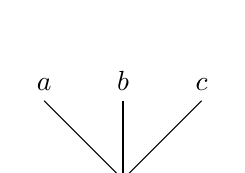
\begin{tikzpicture}
\draw (1,0) -- (0,1) node[above]{$a$} ;
\draw (1,0) -- (1,1) node[above]{$b$} ;
\draw (1,0) -- (2,1) node[above]{$c$} ;
\end{tikzpicture}
\end{center}
Of course, the source of such a map is the source of the first leave and the target is the target of the last leave. The identity maps are represented by the empty trees and the composition consists in joining the roots.
\end{itemize}
\end{defin}

One can repeat the process several times: $F^kC$ is the category with the same objects as $C$ and, as morphisms, the trees of heigh $k$ with maps of $C$ as leaves, which can be composed. The composition consists in joining the roots.\\

There is an obvious functor $\phi$ from $FC$ to $C$: it sends an object to itself ($Obj(FC)=Obj(C)$), and a tree (ie a morphism) to the composition of its leaves (in the previous tree picture, it sends the tree to $a \circ b \circ c$). Define also the obvious functor $:C \rightarrow FC$ which sends an object to itself and a morphism $a$ to the corresponding generator in $FC$, ie:
\begin{center}
\begin{tikzpicture}
\draw (0,0) -- (0,1) node[above]{$a$} ;
\end{tikzpicture}
\end{center}  


Similarly, there are natural functors between $F^2C$ and $FC$; one functor from $F2C$ to $F^2C$ and two functors in the opposite sense:
\begin{itemize}
\item $\phi F: F^2C \rightarrow FC$ reduces the branches between the height 1 and 2, ie:
\begin{center}
\begin{tikzpicture}
\draw (1,0) -- (0,1) ;
\draw (0,1) -- (0,2) node[above]{$a$} ;
\draw (1,0) -- (2,1) ;
\draw (2,1) -- (1,2) node[above]{$b$} ;
\draw (2,1) -- (2,2) node[above]{$c$} ;
\draw (2,1) -- (3,2) node[above]{$d$} ;

\draw (3,1) node{$\mapsto$};

\draw (5,0) -- (4,1) node[above]{$a$} ; 
\draw (5,0) -- (6,1) node[above]{$b \circ c \circ d$} ;
 
\end{tikzpicture}
\end{center}  
\item $F\phi : F^2C \rightarrow FC$ reduces the branches between the height 0 and 1, ie:

\begin{center}
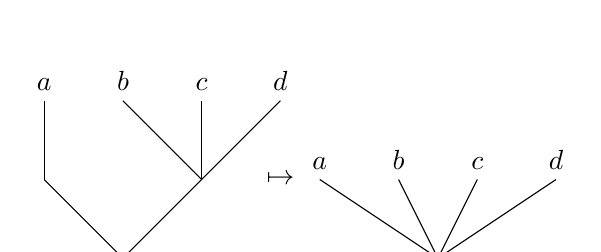
\begin{tikzpicture}
\draw (1,0) -- (0,1) ;
\draw (0,1) -- (0,2) node[above]{$a$} ;
\draw (1,0) -- (2,1) ;
\draw (2,1) -- (1,2) node[above]{$b$} ;
\draw (2,1) -- (2,2) node[above]{$c$} ;
\draw (2,1) -- (3,2) node[above]{$d$} ;

\draw (3,1) node{$\mapsto$};

\draw (5,0) -- (3.5,1) node[above]{$a$} ; 
\draw (5,0) -- (4.5,1) node[above]{$b$} ;
\draw (5,0) -- (5.5,1) node[above]{$c$} ;
\draw (5,0) -- (6.5,1) node[above]{$d$} ;
 
\end{tikzpicture}
\end{center}

\item Define also $\psi :: FC \rightarrow F^2C$:
%\begin{comment}
\begin{center}
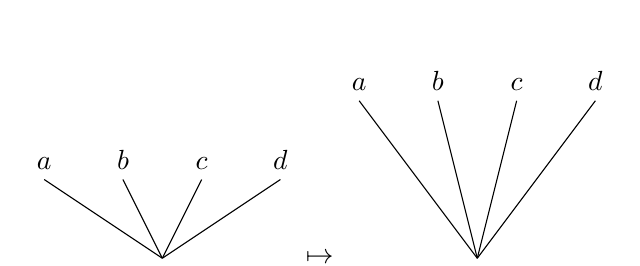
\begin{tikzpicture}
\draw (1.5,0) -- (0,1) node[above]{$a$} ; 
\draw (1.5,0) -- (1,1) node[above]{$b$} ;
\draw (1.5,0) -- (2,1) node[above]{$c$} ;
\draw (1.5,0) -- (3,1) node[above]{$d$} ;

\draw (3.5,0) node{$\mapsto$};

\draw (5.5,0) -- (4,2) node[above]{$a$} ; 
\draw (5.5,0) -- (5,2) node[above]{$b$} ;
\draw (5.5,0) -- (6,2) node[above]{$c$} ;
\draw (5.5,0) -- (7,2) node[above]{$d$} ;
\end{tikzpicture}
\end{center}
%\end{comment}
\end{itemize}

One notices for instance that $(F \phi) \psi=(F \phi) \psi$. One can also continue the process to higher order of free category; one then define in the same way $n$ functors from $F^n C$ to $F^{n-1} C$ and $n$ functors 

\begin{prop}
$(F^{k+1}C)_k$ together with the functors defined above is a simplicial category.
\end{prop} 

Furthermore this new category has the same homotopy type as $C$ (if we consider as a constant simplicial category

\begin{prop}
$(F^{k+1}C)_k \rightarrow C$ (functor unduced by the reduction of the trees) is a weak equivalence of categories (that means that it induces weak equivalences on the simplicial morphisms sets).
\end{prop} 

\begin{proof}[Sketch of the proof.]
Every tree of height $k$ is equivalent (in the homotopy sense) to the tree of same height and with only one leave which is the composition of the leaves.
\end{proof}

\subsubsection{The localization: definitions and first properties}

Along those lines, the morphisms of the localized categories $C[w^{-1}]$ are the tree of height $1$ such that its leaves are a succession of maps of $C$ and of $W$ (quotiented through an equivalence relation). The underlying idea of the standard simplicial localization is to look at the localization of $F^{k} C$ by $F^{k} W$.\\

Then, with few changes in the way of thinking with the respect to what we have in the previous sub-part, one can define: 

\begin{defin}
The (standard) simplicial localization of $(C,W)$ is the simplicial category $L(C,W)$ defined by:
\begin{equation}
L(C,W)_n=F^{n+1}C[(F^{n+1}W)^{-1}]
\end{equation}
\end{defin}

The homotopy groups of this localization is expected to encode the higher homotopy data data of $C$ with respect to $W$. Actually the homotopy relations are basically generated by the relation of two trees which have the same dimension and can be constructed from one same bigger tree. In dimension $0$, it gives the relation: 

\begin{prop}
$\pi_0 (LC(X,Y))=C[W^{-1}](X,Y)$
\end{prop}

\subsubsection{Generalization to simplicial categories}

One can generalise the notion of standard simplicial localization to simplicial categories.

\begin{defin}
If $A$ is a simplicial category, and $V$ a simplicial subcategory. The standard simplicial localization of $A$ with respect to $V$ is the simplicial category:
\begin{equation}
L(A,V)=diag(F^{*+1}A[(F^{*+1}V)^{-1}])
\end{equation} 
\end{defin}

We have something which is close of the old localization of an ordinary category if we take the path-components:
\begin{prop}
$\pi_0 (LB) =(\pi_0 B)[(im \pi_0 V)^{-1}]$
\end{prop}

Finally, let's see one lemma which can be useful:

\begin{lemma}[{\cite[6.3]{dksimplicial}}]
Let $A$ and $B$ two simplicial $C$-categories, $U$ a simplicial subcategory of $A$ and $V$ a simplicial subcategory of $B$, $S: A \rightarrow B$ a functor such that $S(U) \subset V$, and such that $S: A \rightarrow B$ and $S: U \rightarrow V$ are weak equivalence. Then the induced map $LA \rightarrow LB$ is a weak equivalence.
\end{lemma}

The demonstration of this last lemma is more complicated. One needs some machinery, as for instance a model structure on the category of the simplicial categories with the same objects as $C$ (this last category is not small).


\subsection{Hammock localization}

\subsubsection{Definition and first properties}
Let $C$ be a (small) category an $W$ a subcategory. Let's define the simplicial set $L^H (C,W)(X,Y)$ (or shortly $L^H C(X,Y)$); the $k$-simplices are the "reduced hammocks" of width $k$ and any length between $X$ and $Y$:

\[
\xymatrix{& {C_{0,0}} \ar@{-}[r] \ar[d] & {C_{0,1}} \ar[d] \ar@{--}[r] & {C_{0,n-1}} \ar@{-}[d] \ar@{-}[ddr] \\
& {C_{1,0}} \ar@{-}[r] \ar[d] & {C_{1,1}} \ar@{-->}[ddd] \ar@{--}[r] & {C_{1,n-1}} \ar@{-->}[ddd] \ar@{-}[dr] \\
X \ar@{-}[uur] \ar@{-}[ur] \ar@{--}[r] \ar@{-}[ddr] & {C_{2,0}} \ar@{-->}[dd] &&& {Y} \\
                                                                             \\
& {C_{k,0}} \ar@{-}[r] & {C_{k,1}} \ar@{--}[r] & {C_{k,n-1}} \ar@{-}[uur]}
\]

such that:
\begin{enumerate}
\item $n$, the length is $\geq 0$ (if $n=0$, the hammock consists in $k$-times the same morphism from $X$ to $Y$).
\item all vertical maps are in $W$.
\item in each column, all maps go to the same direction and if they go to the left, then they are in $W$.
\item the maps in adjacent columns go in different directions.
\item no column contains only identity maps.
\end{enumerate}

The $i^{th}$ face map $d_i$ consists in omitting the $i^{th}$ row. The $j^{th}$ degeneracy map consists in repeating the $j^{th}$ row. If the resulting hammock is not reduced (it can happen after the application of a face map), then one applies a reduction process:
\begin{enumerate}
\item if a column contains only identity maps, then one omits it.
\item one composes two adjacent columns whenever they go in the same direction
\end{enumerate}

Furthermore, there exists a distinguished vertices $id \in L^HC(X,X)$; if $X,Y$ and $Z$ are object of $C$, then one can also composition law $L^HC(X,Y) \times L^HC(Y,Z) \rightarrow L^H C(X,Z)$ which consists in, in each dimension, compose the hammocks and then reduce the resulting hammock. Then:

\begin{prop}
$L^H (C,W)$ is a simplicial category.
\end{prop}

The morphisms from $X$ to $Y$ of the localized category $C[W^{-1}]$ are the strings of successive arrows (i.e the elements of $L^HC(X,Y)_0$) quotiented by an equivalence relation. This equivalence is generated by the relation I call $\Re$; if $f,g \in L^HC(X,Y)_0$ then $ f \Re g$ if and only if:

\begin{center}
$\exists h \in L^H C(X,Y)_1 , d_0 (h)=f , d_1 (h)=g$
\end{center}

This just means:

\begin{prop}
For two objects $X,Y \in C$, then:
\begin{equation}
\pi_0 (L^H C(X,Y))=C[W^{-1}](X,Y)
\end{equation}
\end{prop}

Therefore, the underlying idea of the hammock localization is to study in a simplicial set the homotopy of string of arrows. Applying the equivalence gives us the usual localization, but makes us loose the higher homotopy data. The hammock localization is the good object to study this higher homotopy data.


\subsubsection{Generalisation to simplicial categories and link with the standard simplicial localization}

One can generalize the hammock localization to simplicial categories; if $B$ is a simplicial category and $V$ a simplicial subcategory (i.e a subcategory of $B$ together with inclusions of simplicial sets $V(X,Y) \rightarrow B(X,Y)$ which commute with the definition of identity and the composition):
\begin{enumerate}
\item $L^H(B,V)$ is an obviously defined bisimplicial category
\item the hammock localization of $B$ with respect to $V$ is $diag L^H(B,V)$
\end{enumerate}

\begin{rmk}
In the above description, one can equivalently use the formalism of simplicial objects over the category of simplicial (small) categories or of bisimplicial enriched categories;
\end{rmk}

There is an important lemma which comes with the description of the hammock of a simplicial category:

\begin{lemma}[{\cite[2.4]{dkcomputing}}]
If $A, B \in sC-cat$ (with the same set objects; see the introduction), and $U \subset A$, $V \subset B$ are simplicial subcategories, if $S : A \rightarrow B$ is a morphism in $sC-cat$ such that $S(U) \subset V$, and if $S:A \rightarrow B$ and $S: U \rightarrow V$ are weak equivalences (of simplicial $C$-categories), then it induces a weak equivalence of $C$-simplicial categories $diag L^H A \rightarrow diag L^H B$
\end{lemma}

This lemma is hard to prove. However, it is the main key for the next proposition:

\begin{prop}
If $C$ is a category and $W$ a subcategory (ordinary categories), then the natural functors:
\begin{equation}
L^H C \leftarrow diag L^H F^{*+1} \rightarrow F^{*+1} [(F^{*+1}W)^{-1}]
\end{equation}
are weak homotopy equivalences (in $sC-cat$).
\end{prop}

\begin{proof}[Ideas in the proof]
We don't make the proof but give its ingredients:
\begin{itemize}
\item the diagonal argument of bisimplicial sets
\item the homotopy lemma just above
\item the comparison lemma: if a category (ordinary) $D$ is freely generated by subcategories $E$ and $W$, then $L^H C \rightarrow C[W^{-1}]$ is a weak equivalence.
\end{itemize}
\end{proof}

So, we have make the link between the standard simplicial localization and the hammock localization. They are homotopy equivalent. Then one uses more the hammock localization as its definition is simpler and because it is simpler to work with it as we will see.

\subsubsection{The $II$-indexing category and hammock graphs}

The $II$ category is defined by:
\begin{enumerate}
\item its objects are the pairs $(S,T)$ of ordered subsets of $\mathbb{N}^*$ ($\mathbb{N}-\{0\}$) such that $S \cup T= \{1,...,|S \cup T|\}$.
\item the morphisms $(S,T) \rightarrow (S',T')$ are the order preserving maps $f: S \cup T \rightarrow S' \cup T'$ such that $f(S) \subseteq S'$ and $f(T) \subseteq T'$
\end{enumerate}

Let $C$ be a category and $W$ a subcategory (ordinary categories).

\begin{defin}
\begin{enumerate}
\item The category of $C$-graphs is defined by:
\begin{enumerate}
\item A $C$-graph is a graph (with directed edges i.e arrows) which set of points is $Obj(C)$.
\item A morphism $G_1 \rightarrow G_2$ of $C$-graph is the data of maps $G_1(X,Y) \rightarrow G_2(X,Y)$ for all $X$ and $Y$, objects of $C$, and where $G_1(X,Y)$ is the set of arrows from $X$ to $Y$ in $G_1$ (idem for $G_2$).
\end{enumerate}
\item the category of $C$-graphs corresponds to the category of $C$-simplicial categories but without the identity mapas and compositions. Indeed, one has the forgetful functor $C-cat \rightarrow C-graph$.
\item A simplicial $C$-graph is a simplicial object over the category of $C$-graph (or equivalently a $C$-graph with simplicial sets of arrows).
\item One has also the forgetful functor $sC-cat \rightarrow sC-graph$.
\item Weak equivalences between simplicial $C$-graphs are just morphisms of simplicial graphs which induce weak homotopy equivalences on the simplicial mapping spaces of arrows between two objects of $C$. This definition is the analogue to the definition of weak equivalence between simplicial $C$-categories.  
\end{enumerate}
\end{defin}

We can define a natural functor $\lambda C : II \rightarrow sC-graph$:
\begin{itemize}
\item An element of $II$ is equivalent to a word made with the letters $C$ and $W^{-1}$ in the way that transform, for example $(\{1,2\},\{3\})$ into $W^{-1} C C$.
\item From such a word, one made a simplicial $C$-graph describe by:
\begin{enumerate}
\item The arrows from $X$ to $Y$ (objects of $C$) are the unreduced hammocks:
\item the length of the hammocks is the length of the word we call $n$
\item The $i^{th}$ column is made of left-directed arrows of $C$ if the $(n+1-i)^{th}$ is $C$
\item The $i^{th}$ column is made of right-directed arrows of $W$ if the $(n+1-i)^{th}$ is $W^{-1}$  
\item These hammocks are organized in a simplicial set through the width as in $L^H C$.
\end{enumerate}
\item All of this is done functorially (because one can reduce parts of the hammocks and add column with the identity. For instance an injection in $II$ leads to the addition of identity maps in the corresponding $C$-graph). Therefore we have created a $II$-diagram in the category $sC-graph$
\item This diagram has a direct limit $lim \lambda C$
\end{itemize}


\begin{prop}
The reduction maps $r_{(S,T)} : \lambda C (S,T) \rightarrow L^H C$ (it is a morphism of the category $sC-graph$) induces a map $lim \lambda C \rightarrow L^H C$ which is a isomorphism.
\end{prop}

So we can see the hammock localization as a limit of graphs with simpler hammocks (of a definite type).

\begin{rmk}
This theory of $II$-diagrams is useful to prove the lemma introduced just above and non proved. However, we won't apply it to this purpose.
\end{rmk}

\subsubsection{Homotopy calculi of fractions}

Let $C$ be a category and $W$ a subcategory (ordinary categories).

\begin{defin}
$(C,W)$ is said to admit:
\begin{enumerate}
\item a homotopy calculus of (two-sided) fractions if, for every pairs $i,j >0$ the obvious maps in $sC-graph$ (adding a column with only identity):
\begin{equation}
W^{-1}C^{i+j}W^{-1} \rightarrow W^{-1}C^iW^{-1}C^jW^{-1}
\end{equation}
and
\begin{equation}
W^{-1}W^{i+j}W^{-1} \rightarrow W^{-1}W^i W^{-1} W^j W^{-1}
\end{equation}
are both weak equivalences (we consider the words as graph as seen just before).
\item a homotopy calculus of left fractions if, for every pairs $i,j >0$ the obvious maps in $sC-graph$:
\begin{equation}
W^{-1}C^{i+j} \rightarrow W^{-1}C^iW^{-1}C^j
\end{equation}
and
\begin{equation}
W^{-1}W^{i+j} \rightarrow W^{-1}W^i W^{-1} W^j
\end{equation}
are both weak equivalences.
\item a homotopy calculus of right fractions is defined in an analogue way.
\end{enumerate}
\end{defin}

The usefulness of the previous definition is due to the following proposition:

\begin{prop}[{\cite[6.2]{dkcomputing}}]
\begin{enumerate}
\item If $(C,W)$ admits a homotopy calculus of (two-sided) fractions, then the reduction maps
\begin{equation}
W^{-1}CW^{-1} \rightarrow L^H (C,W), W^{-1}WW^{-1} \rightarrow L^H (W,W)
\end{equation}
are weak equivalences.
\item one has the same kind of statement for the homotopy calculus of left or right fractions.
\end{enumerate}
\end{prop}

So, if the category admits a homotopy calculus of fractions, then the homotopy of its hammock localization is then much simpler to describe as we have only to consider hammocks of a certain shape.

\subsubsection{Case where the homotopy calculus is used}

\begin{defin}
$(C,W)$ admits a calculus of left fractions if:
\begin{enumerate}
\item For each diagram $\xymatrix{{X'} & X \ar[l]^u \ar[r]^f & Y}$ of $C$ with $u \in W$, there exists in $C$ a diagram $\xymatrix{{X'} \ar[r]^{f'} & {Y'}  & Y \ar[l]_v}$ with $v \in W$ and such that $v \circ f = f' \circ u$
\item If $f,g : X \rightarrow Y$ are morphisms of $C$ and $u :X' \rightarrow X$ is in $W$, and they are such that $f \circ u = g \circ u$, then there exists $v \in W$ such that $v \circ f= v \circ g$.
\end{enumerate} 
\end{defin}

Note that if $(C,W)$ admits a calculus of left fractions and if it is such that:
\begin{center}
if $f,g$ are morphisms of $C$ such that one can define $f \circ g$, and if two of the three morphisms $f$, $g$, and $f \circ g$ are in $W$, then the third is in $W$ 
\end{center}
then $(W,W)$ also admits a calculus of left fractions.\\


We have two important results about the calculus of left fractions:

\begin{prop}
If $(C,W)$ and $(W,W)$ admit a calculus of left fraction, then $(C,W)$ admits a homotopy calculus of left fraction.
\end{prop}

\begin{prop}
If $(C,W)$ and $(W,W)$ admit a calculus of left fraction, then the natural map:
\begin{equation}
L^H C \rightarrow \pi_0 L^H C = C[W^{-1}]
\end{equation}
is a weak equivalence of simplicial categories.
\end{prop}

Now, a final proposition which makes the hammock localization very useful in the frame of model category; here $M$ is a model category, $W$ refers to the weak equivalences, $M^c$ to the cofibrant subcategory, $M^f$ to the fibrant subcategory and $M^{cf}$ to the fibrant-cofibrant subcategory.

\begin{prop}
The pairs $(M,W)$, $(M^{c},W^{c})$, $(M^{f},W^{f})$ and $(M^{cf},W^{cf})$ admit homotopy calculi of two-sided fractions.
\end{prop}

\section{Homotopy simplicial category and conclusion}

We won't prove the following theorem which is the conclusion of our discussion:
\begin{thm}[{\cite[Thm. 4.4]{dkfunction}}]
Let $M$ be a model category. For any two objects $X,Y$ of $M$, if $X^*$ is a cosimplicial resolution of $X$ and $Y_*$ is a simplicial resolution of $Y$, then the simplicial sets $diag M(X^*,Y_*)$ and $L^H(X,Y)$ have the same homotopy type.
\end{thm}

\section{Complements to Chapter 2}

\subsection{Bisimplicial set}

\begin{defin}
A bisimplicial set is equivalently:
\begin{enumerate}
\item A simplicial object over the category $sSet$
\item A functor $(\Delta \times \Delta)^{op} \rightarrow Set$
\item A functor $\Delta^{op} \times \Delta^{op} \rightarrow Set$
\item A family of sets $(X_{n,m})_{(n,m) \in \mathbb{N}^2}$ together with two types of face maps and degeneracies such that the two simplicial structures commute.
\end{enumerate}
\end{defin}


The diagonal of a bisimplicial set is the obvious simplicial set made with the sets $X_{n,n}$, the face maps $X(d_i,d_i)$ and the degeneracies $X(s_j,s_j).$

\begin{comment}
\subsection{Auto equivalenc monoid}

\begin{defin}
A simplicial monoid is a simplicial obect in the category $Mon$ of monoids.
\end{defin}

\begin{defin}
Let $M$ be a model category with $W$ the subcategory of weak equivalences. Let $X$ an object of $M$. Then, the homotopy automorphisms complex $haut_{L^HM}X$ is the simplicial submonoid of $L^HM(X,X)$ which corresponds to the components which are invertible in $\pi_0 L^HM(X,X)$. In other words,
\begin{equation}
\forall n, haut_{L^HM}X_n=.....
\end{equation}
\end{defin}
\end{comment}

\nocite{hirschhorn, fromHAtoHAG, gj, gz, htt}
\printbibliography[heading = local]

\end{refsection}

\chapter{Quasi-categories}

\begin{refsection}

This chapter is intented to give an intuition of what $(\infty,1)$-categories are and to present an informal introduction to one of theirs models, namely quasi-categories (sometimes called weak Kan complexes). We show how some basic concepts of ordinary category theory extend to the $(\infty,1)$-categorical context, and specifically to the model of quasi-categories.

\begin{flushright}
Valerio Melani
\end{flushright}

\section{Intuition and first models}

We start by trying to give some intuition for what these $(\infty,1)$-categories are, and how one could search for a suitable formalism to describe them. Next, we will concentrate our efforts in starting to understand one of the different models for $(\infty,1)$-categories, namely the so-called \emph{quasi-categories}.

Heuristically speaking, an $(\infty,1)$-category is of course first of all an $\infty$-category. This means that we have objects, morphisms between objects, 2-morphisms between morphisms, 3-morphisms between 2-morphisms, and so on. Put this way, this is not yet a very precise object, because actually we want to have some kind of compositions between these $k$-morphisms, and these compositions must of course have some nice properties that fit our general intuition. This is (one of the) main reason why higher category theory has a reputation of being overcomplicated and messy; for a general discussion about the problems of defining higher categories, we recommend for example the lecture of ???.

Luckily we will not have to go into these kind of details, as we just want to describe the special case of $(\infty,1)$-categories, who are just $\infty$-categories whose $k$-morphisms are invertible for $k>1$. This sensibly simplifies our task : generalizations of classical ideas from (ordinary) category theory becomes much more complicated if we allow the existence of non-invertible $k$-morphisms (k>2).

That being said, where should we start looking for a possible model of $(\infty,1)$-categories? We observe that if $x$ and $y$ are two "objects" of a wanna-be $(\infty,1)$-category, the morphisms between them form an $\infty$-category whose all morphisms are invertible, even the $1$-morphisms ; this is what is called an $\infty$-groupoid.
$\infty$-groupoids have been extensively studied under the false name of topological spaces. In fact, a general principle of higher category theory (the \emph{homotopy hypothesis}) states exactly that $\infty$-groupoids and topological spaces are same thing, homotopically speaking. To be more precise, if we are given a topological space $X$, we can easily associate to it an $\infty$-groupoid : the classical construction of the fundamental groupoid of a topological space can be extended in a natural way to get an $\infty$-groupoid $\pi_{\infty}X$ as follows. The objects of $\pi_{\infty}X$ are the points of $X$. If $x,y \in X$, then the morphisms from $x$ to $y$ in $\pi_{\infty}X$ are the continuous paths in $X$ starting at $x$ and ending at $y$. The $2$-morphisms are homotopies of paths, the $3$-morphisms are homotopies between homotopies of paths, and so on all  the way to $\infty$. What we get is an $\infty$-groupoid who remembers all the homotopical information of $X$. The homotopy hypothesis tells us the converse : every $\infty$-groupoid is of the form $\pi_{\infty}X$ for some topological space $X$.

So saying that morphisms between two objects of an $\infty$-category form an $\infty$-groupoid is the same that saying that they form a topological space. We can therefore try and give the following definition.

\begin{defin}
An $\infty$-category is a \emph{topological category}, i.e. a category which is enriched over the category of topological spaces.
\end{defin}

But in homotopy theory, there are many equivalent ways to describe spaces: using one of them, we are led to the following different interpretation of an $\infty$-category.

\begin{defin}
An $\infty$-category is a \emph{simplicial category}, i.e. a category which is enriched over the category of simplicial sets.
\end{defin}

These are two definitions who can be both used as a foundation for higher category theory. They look simple enough, but taking one of these approaches lead to some technical difficulties that we would like to avoid. A first alternative definition of an $\infty$-category will be given in the next section.

\section{Quasi-categories}

There are two classes of examples we certainly wish to have in any theory of $\infty$-categories:
\begin{itemize}
\item $\infty$-groupoids (i.e. spaces), as they are of course a special case of $\infty$-category ;
\item ordinary categories, as they can be thought as $\infty$-categories where for $k >1$ the only $k$-morphisms are the identities.
\end{itemize}

So the question is to find a formalism in containing both these theories. And one possible answer is the theory of simplicial sets. Given a topological space $X$, the classical construction of his singular complex $\text{Sing}(X)$ is a simplicial set who determines $X$ up to weak homotopy equivalence. The simplicial set $\text{Sing}(X)$ has the important property of being a \emph{Kan complex}

\begin{defin}
A simplicial set $S$ is a \emph{Kan complex} if every map $\Lambda_k^n \to S$ extends to a map $\Delta^n \to S$.
\end{defin}

It is quite clear that if $X$ is a topological space, then $\text{Sing}(X)$ is a Kan complex : this is due to the fact the horns are retracts of the simplex $\Delta^n$ in the world of topological spaces. The converse is also true : Kan complexes are topological spaces, in the sense that just as $\infty$-groupoids they are models for homotopy types.
Now given a category $\mathcal C$, we can construct a simplicial space $N(\mathcal C)$ called the \emph{nerve} of $\mathcal C$ as follows. We just let the $n$-simplices of $N(\mathcal C)$ be the strings of $n$ composable morphisms of $\mathcal C$. If you think about it, this simplicial set knows all about the category $\mathcal C$, it just encodes the information in another language. But what kind of simplicial set do we get? The following proposition gives us the answer.

\begin{prop}
A simplicial set $S$ is isomorphic to the nerve of some category if and only if every map $\Lambda_k^n \to S$ with $0<k<n$ extends uniquely to a map $\Delta^n \to S$.
\end{prop}

Knowing that we are trying to generalize spaces and categories, the following definition should not surprise us.

\begin{defin}
A \emph{quasi-category} is a simplicial set $S$ in which every map $\Lambda_k^n \to S$ with $0<k<n$ extends to a map $\Delta^n \to S$.
\end{defin}

Part of the literature on the subject refers to quasi-categories as \emph{weak Kan complexes}, to stress the analogy with the precedent notion.
We state that quasi-categories are a good model for the theory of $(\infty,1)$-categories. The rest of this notes is devoted to convincing us of this fact.

\subsection{Mapping spaces}

As we said earlier, we know we should be able to find a space (or a good homotopy types) between any two objects of a $(\infty,1)$-categories. This is easy in the world of topological (or simplicial) categories. It is less obvious in our setting of quasi-categories.

We should now point out that there are actually explicit adjoint functors that establish an equivalence between the theory of simplicial categories that of quasi-categories. So the problem of finding mapping spaces in a quasi-category could be bypassed by taking a simplicial category which is equivalent to our quasi-category, and take mapping spaces there. Here we try to avoid this point of view, partly because the two adjoint functors are quite complicated, and the resulting mapping spaces could be quite obscure. Details can be found on \cite{htt}.

The question of how to define mapping spaces in quasi-categories is of independent interest, and has been studied in \cite{DS}. Here we just show one way of defining them.

If $x$ and $y$ are objects of an $(\infty,1)$-category $\mathcal C$ (i.e. they are vertices of $\mathcal C$ as a simplicial set) we define a simplicial set $\Hom^R(x,y)$, called the space of right morphisms from $x$ to $y$. This is done by letting $\Hom_{SSet}(\Delta^n,\Hom^R(x,y))$ be the set of all maps $f: \Delta^{n+1} \to \mathcal C$ such that $f$ sends the $(n+1)$-th vertex to $y$ and the first $n$ to x (as a degenerate simplex).

We can prove that is what we were looking for :  $\Hom^R(x,y)$ is a Kan complex, and it is equivalent to other more abstract definitions of the mapping space.



\subsection{The homotopy category}

We now define the homotopy category of a quasi-category $\mathcal C$. This is to be thought as the underlying ordinary category of $\mathcal C$, who remembers only low homotopical information and forgets about the higher one. 

Again, if we think in terms of topological (or simplicial) categories, all is easy : we can take the set of morphisms between two objects $x,y$ to be the $\pi_0$ of the topological space (or simplicial set) $\Hom (x,y)$. Now that we dispose of mapping spaces in the setting of quasi-categories, we can do the same.

\begin{defin}
If $\mathcal C$ is a  quasi-category, his homotopy category $h\mathcal C$ is the category whose objects are the objects of $\mathcal C$ and whose morphisms are the path-connected components of the mapping spaces of $\mathcal C$.
\end{defin}

Another way to describe it is to notice that the nerve functor defined earlier in the text admits a left adjoint $h: \sset \to \Cat$, doing exactly what we want: it only keeps the 1-categorical information contained in $\mathcal C$. See Theorem \ref{thm nerve adjunction 1} for a proof of this statement.

Let's get a more explicit understanding of what the homotopy category concretely is: given two vertices $x,y \in \C$ and two edges $f,g : x \to y$ (meaning that the edges start at $x$ and end at $y$), we say that $f$ and $g$ are homotopic if there is a $2$-simplex in $\mathcal C$ who has $f$ as the $0\to 1$ edge, $g$ as the $0\to 2$ edge, and the degenerate edge at $y$ as $1 \to 2$ edge. (This is very clear if you try and draw the diagram).

The fact that $\mathcal C$ is a quasi-category means that ``being homotopic'' is an equivalence relation. The homotopy category is now just the category whose objects are the the objects of $\mathcal C$ and whose morphisms are the equivalence classes of edges of $\mathcal C$.



\subsection{Functors between quasi-categories}

We now describe the category of functors between quasi-categories. This is one of the cases in which some technical problem with the topological (and simplicial) categories arise. In any reasonable model, we expect to be able to construct an $(\infty,1)$-category of functors between two $(\infty,1)$-categories. The problem is that there is not an obvious way to give a good definition of this category in the setting of topological (simplicial) category.

Here quasi-categories give their best, and the definition are much easier.

\begin{defin}
Given two quasi-categories $\mathcal C$ and $\mathcal D$, the simplicial set $\Hom_{SSet}(\mathcal C,\mathcal D)$ is called the \emph{$(\infty,1)$-category of functors} from $\mathcal C$ to $\mathcal D$.
\end{defin}

Here we used the fact that the category of simplicial sets has internal Hom objects, and we are defining the maps of quasi-categories as maps of simplicial sets. Notice that $\Hom_{SSet}(\mathcal C,\mathcal D)$ has the right to be called an $(\infty,1)$-category thanks to the following proposition.

\begin{prop}
If $\mathcal C$ is a quasi-category, then the simplicial set $\Hom_{SSet}(S,\mathcal C)$ is a quasi-category for every simplicial set $S$.
\end{prop}

In particular, a functor between quasi-categories is an equivalence if and only if it is essentially surjective on objects and induces homotopy equivalences between mapping spaces.


\subsection{Limits and colimits}

In this section we explain how to define limits and colimits in the setting of quasi-categories.

In the same way that limits and colimits in an ordinary category can be defined using the definition of limits and colimits in the category of sets, limits and colimits in a quasi-category can be defined using the notion of homotopy limits and colimits in the model category of spaces.
If we want to be concise, we could give the following definition: given a functor $I \to \mathcal C$ between two $(\infty,1)$-categories, its limit and colimit (if they exist) are determined by asking that the natural maps

\begin{gather*}
\Hom(X, \lim F(i)) \to \text{holim }\Hom(X,F(i)) \\
\Hom(\text{colim }F(i),X) \to \text{hocolim } \Hom(F(i),X)
\end{gather*}

are weak equivalences of spaces that are natural in $X$.


\subsection{Model structure}

In order to prove later that the different models of $(\infty,1)$-categories are equivalent, we now give the definition of a model structure on the category of simplicial sets which is different from the standard one.

%In order to do this, we let $h_0(S,S')$ be the set of isomorphism classes of objects in the homotopy category of $\Hom(S,S')$.
We say then that a map of simplicial sets $S \to S'$ is a \emph{weak categorical equivalence} if the induced map $\Hom(S',X) \to \Hom(S,X)$ is an equivalence of quasi-categories for any quasi-category $X$.

\begin{thm}[Joyal] There exists a model structure on the category $SSet$ of simplicial sets with the following properties:
\begin{itemize}
\item weak equivalences are the weak categorical equivalences ;
\item cofibrations are just monomorphisms of simplicial sets ;
\item the fibrant objects are precisely the quasi-categories.
\end{itemize}
\end{thm}

In particular, this means that for this model structure weak equivalences between fibrant objects are precisely equivalences of quasi-categories.

\nocite{bergner1}
\printbibliography[heading = local]

\end{refsection}

\chapter{Segal spaces and Segal categories}

\begin{refsection}

In this talk, we will discuss two models for $(\infty,1)$-categories in detail, namely complete Segal spaces and Segal categories. We will focus on the homotopy theory of these two models, as well as briefly sketching their relations to other models.

\begin{flushright}
Yan Zhao
\end{flushright}

\section{Preliminaries}
\subsection{Simplicial space}
In this paper, a {\bf space} will always refer to a simplicial set. Let $\mathcal S$ be the category of spaces, which we endow with the standard model category structure, i.e. a weak equivalence is a homotopy weak equivalence, a cofibration is an injection and a fibration is a Kan fibration. Let $\Delta^n$, $\partial\Delta^n$ and $\Lambda^n_k$ be the standard $n$-simplex, the boundary of the standard $n$-simplex and the $k$-th horn of the $n$-simplex (boundary of the $n$-simplex with the $k$-th face removed) respectively. For any $X,Y\in\cal S$, the mapping space is the function complex $\Map_\mathcal S(X,Y)$, where the $n$-simplex can be given by the set of all maps $X\times\Delta^n\to Y$.

Let $\Delta\subset\Cat$ be the category of categories consisting of objects $[n]$, with the usual face and degeneracy maps $d^i$ and $s^i$. A {\bf simplicial space} is thus a functor $X:\Delta^{op}\to\mathcal S$, which sends $[n]\mapsto X_n$, with face and degeneracy maps $d_i:X_n\to X_{n-1}$ and $s_i:X_n\to X_{n+1}$. Let $s\mathcal S$ be the category of simplicial spaces.

Note that a simplicial space can also be seen as a bisimplicial set $X:\Delta^{op}\times\Delta^{op}\to \Set$ with two sets of arrows $d_i$ and $s_i$. Let ${\mathcal S}^{(2)}$ denote the category of bisimplicial sets. It is clear that there is an isomorphism of categories between $s\mathcal S$ and ${\mathcal S}^{(2)}$. The former notation is more convenient for the discussion of homotopy theory while the latter in the comparison theorems between different models of $\infty$-categories. We will freely interchange between the two characterisations.

We can identify $\mathcal S$ as a full subcategory of $s\mathcal S$ by sending each simplicial set $K$ to the constant simplicial space $[n]\mapsto K$ with $d_i$ and $s_i$ being the identity maps. The category $s\mathcal S$ can be enriched over simplicial sets in a compatible way with the enrichment of $\mathcal S$. For any $X,Y\in s\mathcal S$, we have the function complex $\Map_{s\mathcal S}(X,Y)$, where each $n$-simplex is the set of simplicial maps $X\times\Delta^n\to Y$.

Let $F(k)$ be the simplicial space defined by $[n]\mapsto \Delta([n],[k])$. where the set of morphisms $\Delta([n],[k])$ in $\mathcal S$ is taken as a discrete simplicial set. $F(k)$ is a $k$-th space functor, in the sense that there is an isomorphism
$$\Map_{s\mathcal S}(F(k),X)\cong X_k$$
of simplicial sets which is natural with respect to $d^i:F(k)\to F(k+1)$ and $s^i:F(k)\to F(k-1)$.
Let $\partial F(k)$ be the largest subobject of $F(k)$ not containing the identity map $\iota:[k]\to[k]$. It can easily be seen that $\partial F(k)$ is generated by the faces $d_i\iota\in\Delta([k-1],[k])$. We denote by $\partial X_k$ the mapping space $\Map_{s\mathcal S}(\partial F(k),X)$. The inclusion $\partial F(k)\hookrightarrow F(k)$ induces a map $X_k\to\partial X_k$.

\begin{prop}
The category of simplicial spaces $s\cal S$ is catesian closed, that is, for $X,Y\in s\mathcal S$, there exists an internal hom-object $Y^X$ with a natural isomorphism
$$s\mathcal S(X\times Y,Z)\cong s\mathcal S(X,Z^Y).$$
\end{prop}
\begin{proof}
Let $(Y^X)_k=\Map_{s\mathcal S}(X\times F(k),Y)$.
\end{proof}

\subsection{Reedy model category structure on $s\mathcal S$}
\begin{thm}
There exists a model structure on $s\mathcal S$ where $f:X\to Y$ is a
\begin{enumerate}
\item weak equivalences if $f_k:X_k\to Y_k$ are degree-wise weak equivalences;
\item cofibrations if $f_k$ are degree-wise cofibrations;
\item fibrations if the induced map
\begin{equation} \label{Reedyfib}
X_k\to Y_k\times_{\partial Y_k}\partial X_k
\end{equation}
are fibrations.
\end{enumerate}
\end{thm}
\begin{proof}
See \cite[IV.3.2]{gj}.
\end{proof}

This is called the {\bf Reedy model structure} on the category of simplicial spaces. It is given by the Reedy model structure construction on the model category $\mathcal S$ and the Reedy category $\Delta$. Note that all simplicial spaces are cofibrant and a simplicial space $X$ is Reedy fibrant iff
$$X_k\to\partial X_k,\qquad k\ge 0.$$

As with the standard model structure on the category of simplicial sets, the Reedy model category structure is cofibrantly generated \cite{dhk}, that is, there exist sets of generating cofibrations and generating trivial cofibrations such that trivial fibrations (fibrations, respectively) are characterised by the right lifting property with respect to the set of generating cofibrations (generating trivial cofibrations). The generating cofibrations are
$$\partial F(k)\times \Delta^l\sqcup_{\partial F(k)\times\partial\Delta^l}F(k)\times\partial\Delta^l\to F(k)\times\Delta^l,\qquad k,l\ge0$$
and the generating trivial cofibrations are
$$\partial F(k)\times \Delta^l\sqcup_{\partial F(k)\times\Lambda^l_t}F(k)\times\Lambda^l_t\to F(k)\times\Delta^l,\qquad k\ge0,0\le t\le l.$$

\begin{defin}
A model category structure on $\cal C$ is compatible with cartesian closure if for any cofibrations $i:A\to B$, $j:C\to D$ and fibration $p:X\to Y$, either (and hence both) of the equivalent characterisations hold:
\begin{enumerate}
\item the induced map $A\times D\sqcup_{A\times C}B\times C\to B\times D$ is a cofibration, which is trivial if either $i$ or $j$ is; or
\item the induced map $X^B\to X^A\times_{Y^A}Y^B$ is a fibration, which is trivial if either $i$ or $p$ is.
\end{enumerate}
\end{defin}

\begin{prop}
$s\mathcal S$ with the Reedy model structure is compatible with cartesian closure.
\end{prop}
\begin{proof}
It suffices to check condition (i). This holds since cofibrations and weak equivalences are defined degree-wise and the standard model structure on $\mathcal S$ is compatible with cartesian closure (in $\mathcal S$, the induced map in (i) is an anodyne extension).
\end{proof}

In particular, this implies that given any cofibration (inclusion) $A\hookrightarrow B$ and $X$ fibrant, we have a fibration $\Map_{s\mathcal S}(B,X)\to\Map_{s\mathcal S}(A,X)$, which is trivial if $A\hookrightarrow B$ is.

Recall the definition of a proper model category.
\begin{defin}
A model category is proper if
\begin{enumerate}
\item the pushout of a weak equivalence along a cofibration is a weak equivalence; and
\item the pullback of a weak equivalence along a fibration is a weak equivalence.
\end{enumerate}
\end{defin}

\begin{prop}
$s\mathcal S$ is a proper model category.
\end{prop}
\begin{proof}
$\mathcal S$ is a proper model category. Since cofibrations and weak equivalences are degree-wise, condition (i) follows trivially.
Condition (ii) follows from the fact that under the Reedy model category structure, if all objects are cofibrant, then all fibrations are also degree-wise fibrations. Indeed, since $\partial F(k)$ is cofibrant and the Reedy model structure is compatible with cartesian closure, the cofibration $\emptyset\to\partial F(k)$ and the fibration $X\to Y$ induces a fibration of internal hom-objects
$$X^{\partial F(k)}\to Y^{\partial F(k)}\times_{Y^\emptyset}X^\emptyset\cong Y^{\partial F(k)}$$
This thus induces a fibration on the 0-spaces $\partial X_k\to\partial Y_k$. Pulling back along $Y_k\to\partial Y_k$ and composing with (\ref{Reedyfib}), we get a fibration
$$X_k\to\partial X_k\times_{\partial Y_k}Y_k\to Y_k.$$
\end{proof}

We state a property of proper model categories:

\begin{prop}\label{hompullback}
Let $\cal C$ be a proper model category. Then, the pushout along a cofibration is a homotopy pushout and the pullback along a fibration is a homotopy pullback.
\end{prop}
\begin{proof}
See \cite[Prop A.2.2.4]{htt}.
\end{proof}

\section{Segal spaces}
In this section, we will construct our first model of $(\infty,1)$-categories, the complete Segal spaces. Complete Segal spaces have an explicit homotopy structure, which Rezk described as the study of homotopy theory of homotopy theories. For most of this section, we will give explicit constructions following Rezk's paper \cite{rezk}.

\subsection{The Segal conditon}
The Segal condition is a modification of the $\Delta$-space defined by Graeme Segal, which is a simplicial space $X$ in which $X_n$ is naturally weakly equivalent to $(X_1)^n$. In the Segal condition, we allow the $0$-space to be more than a single point.

For $0\le i<k$, let $\alpha^i:[1]\to [k]$ be the map sending $[0,1]\mapsto [i,i+1]$. Let $G(k)\subset F(k)$ be the simplicial subspace generated by $\alpha^i\in F(k)_1$. Equivalently, $\alpha^i$ induces a map $F(1)\to F(k)$ and we define $G(k)$ to be
$$G(k)=\cup_{i=0}^{k-1}\alpha^iF(1)\subset F(k).$$
The inclusion $\phi^k:G(k)\hookrightarrow F(k)$ induces a map $\phi_k=\Map_{s\mathcal S}(\phi^k,X):\Map_{s\mathcal S}(F(k),X)\cong X_k\to\Map_{s\mathcal S}(G(k),X)$. We can check that
$$\Map_{s\mathcal S}(G(k),X)\cong X_1\times_{X_0}\cdots\times_{X_0}X_1=\lim(X_1\xrightarrow{d_0}X_0\xleftarrow{d_1}X_1\xrightarrow{d_0}\cdots\xrightarrow{d_0}X_0\xleftarrow{d_1}X_1)$$
with $k$ copies of $X_1$.

\begin{defin}
We say that a simplicial space $X$ satisfies the Segal condition if
\begin{equation} \label{segal}
\phi_k:X_k\to X_1\times_{X_0}\cdots\times_{X_0}X_1
\end{equation}
is a weak equivalence for each $k\ge 2$.
\end{defin}

Therefore, two simplicial spaces satisfying the Segal condition are defined up to weak equivalence by their 0-th and 1-st spaces.

We can define a simplicial enriched structure associated to a simplicial space satisfying the Segal condition:
\begin{defin}\label{simpcat}
Let $W$ be a simplicial space. Define $\Ob W=(W_0)_0$ to be the vertices of $W_0$ and for any $x,y\in\Ob W$, we define $\map_W(x,y)$ to be the fiber of the map $(d_1,d_0):W_1\to W_0\times W_0$ at the point $(x,y)\in W_0\times W_0$. The identity map is defined to be $\id_x=s_0x\in\Map_W(x,x)$.
\end{defin}
In general, for a simplicial space $W$ satisfying the Segal condition, $\map_W(x,y)$ is not fibrant, so we cannot define a homotopy equivalence on the simplicial set. However, requiring $\map_W(x,y)$ to be fibrant for all $(x,y)$ (eg. by requiring $(d_1,d_0):W_1\to W_0\times W_0$ to be a fibration) is still not sufficient. We also want the following condition: we want a homotopy relation that is well-defined up to changing of the end points by a path in $(W_0)_1$, that is, if $[x],[y]\in\pi_0(W_0)$ are the path-components of $x$ and $y$, then we want $\map_W([x],[y])$ to be defined in some way and a homotopy equivalence relation on it.

It turns out that an appropriate condition to impose is Reedy fibrancy.
\begin{defin}
A Segal space is a Reedy fibrant simplicial space satisfying the Segal condition.
\end{defin}
Note that since a Segal space $W$ is fibrant and $G(k)\subset F(k)$ is a cofibration, the map $\phi_k$ is a fibration for all $k$. Similarly, $d_0,d_1:W_1\to W_0$ are fibrations, hence $(d_1,d_0):W_1\to W_0\times W_0$ is a fibration and $\map_W(x,y)$ are fibrant. Furthermore, $W_1\times_{W_0}\cdots\times_{W_0}W_1$ is a homotopy fibre product.

In particular, $W_0$ is fibrant as $W$ is fibrant, and compositions of the fibrant maps in the previous paragraph gives us that $W_k$ is fibrant for all $k$. Hence, we can view a Segal space as a Reedy fibrant simplicial object in the category of topological spaces satisfying the Kan condition. This view is more convenient for geometrical examples. For a complete description, see \cite{lurietft}.

\begin{eg}
Every discrete simplicial space ($W_k$ is discrete for each $k$) is Reedy fibrant. Hence, it is a Segal space iff it satisfies the Segal condition. Indeed, if a discrete simplicial space satisfies the Segal condition, then $\phi_k$ will be isomorphisms.
\end{eg}

\subsection{Examples of Segal spaces}\label{egss}
\subsubsection{Classification diagram of categories}
We denote by $\mathrm{nerve}(C)$ the nerve of a category $C$, that is, the simplicial set with $n$-simplices given by a chain of composable morphisms
$$c_0\to\ldots\to c_n.$$
\begin{prop}\label{nerve}
$\mathrm{nerve}([n])=\Delta^n$. For any categories $C$ and $D$, there are natural isomorphism $\mathrm{nerve}(C\times D)\cong\mathrm{nerve}(C)\times\mathrm{nerve}(D)$ and $\mathrm{nerve}(D^C)\cong\mathrm{nerve}(D)^{\mathrm{nerve}(C)}$. The nerve functor gives a full embedding $\mathrm{nerve}:{\cal C}at\to\mathcal S$.
\end{prop}

Let $C$ be a category and $W\subset C$ a subcategory such that $\Ob W=\Ob C$. 

\begin{defin}
Let $(C,W)$ be a category with its subcategory of weak equivalences. We say that a morphism $f$ is a {\bf weak equivalence} if $f\in W$.

Let $D$ be any other category. For any two functors $f,g\in C^D$, we say that a natural transformation $f\xrightarrow{\alpha}g$, we say that $\alpha$ is a {\bf weak equivalence} if $\alpha d \colon f(d) \to g(d)$ is a weak equivalence for all $d\in\Ob D$. Let $\mathrm{we}(C^D)\subset C^D$ be the subcategory of all weak equivalences.

The {\bf classification diagram} of $(C,W)$ is defined to be the simplicial space $N(C,W)$ where
\[
N(C,W)_m=\mathrm{nerve}\,\mathrm{we}(C^{[m]}).
\]
\end{defin}
It is convenient to view an $n$-simplex of $N(C,W)_m$ as a diagram
\[
\begin{matrix} c_{00}&\to&\cdots&\to&c_{0m}\\\downarrow&&&&\downarrow\\\vdots&&&&\vdots\\\downarrow&&&&\downarrow\\c_{n0}&\to&\cdots&\to&c_{nm}
\end{matrix}
\]
where the vertical arrows are weak equivalences.

We consider some special cases:
\begin{eg}\label{nerveeg}
\begin{enumerate}
\item Let $C_0\subset C$ be the subcategory consisting of all objects and only the identity morphisms. Then, $\mathrm{discnerve}\,C=N(C,C_0)$ is known as the {\bf discrete nerve}. In particular $\mathrm{discnerve}([n])=F(n)$. However, note that equivalent categories may not give weakly-equivalent discrete nerves.

\item Let $\mathrm{iso}\,C\subset C$ be the subcategory consisting of all objects and all invertible morphisms in $C$ (i.e. the maximal subgroupoid of $C$). The {\bf classifying diagram} of $C$ is defined to be $NC=N(C,\mathrm{iso}\,C)$.
\end{enumerate}
\end{eg}

\begin{prop}
The classifying diagrams $\mathrm{discnerve}\,C$ and $NC$ of a category $C$ are Segal spaces.
\end{prop}
\begin{proof}
(i) Note that $(\mathrm{discnerve}\,C)_m\cong(\mathrm{nerve}\,C)_m$ are discrete simplicial sets, so it is clear that $\mathrm{discnerve}\,C$ satisfies the Segal condition. Furthermore, all discrete simplicial spaces are Reedy fibrant.

(ii) Let $I[n]$ denote the category with $n+1$ objects with a unique isomorphism between each pair of objects. An $n$-simplex in $NC_m$ can thus be seen as a functor $[m]\times I[n]\to C$. It is then easy to see that there is a natural isomorphism
$$NC_m\cong NC_1\times_{NC_0}\cdots\times_{NC_0}NC_1.$$
To show that $NC$ is Reedy fibrant, we need to show that the maps $l_m:NC_m\to\partial NC_m$ are fibrations for $m\ge0$. They are easy to check using the above representation of $n$-simplices in $NC_m$. Indeed, $l_m$ is an isomorphism for $m\ge 3$.
\end{proof}

We obtain a result similar to Prop.~\ref{nerve}:
\begin{prop}\label{nerveprop}
Let $C$ and $D$ be categories. There are natural isomorphisms $N(C\times D)\cong NC\times ND$ and $N(D^C)\cong ND^{NC}$. More generally, given $\mathrm{iso}\,D\subset W\subset D$ a subcategory,
\begin{equation} \label{nfuncat}
N(D^C,\mathrm{we}(D^C))\cong N(D,W)^{NC}\cong N(D,W)^{\mathrm{discnerve}\,C}.
\end{equation}
The functor $N:{\cal C}at\to s\mathcal S$ is a full embedding of categories. $F:C\to D$ is an equivalence of categories iff $NF$ is a weak equivalence of simplicial spaces.
\end{prop}
\begin{proof}
See \cite[Thm 3.7, Prop 3.11]{rezk}.
\end{proof}

\subsubsection{Classification space of a closed model category}
Let $C=M$ be a closed model category and $W\subset M$ be its subcategory of weak equivalences. As noted above, we have a simplicial space $N(C,W)$. $N(C,W)$ is in general not Reedy fibrant. However, we can take a functorial Reedy fibrant replacement of it, for example, by the small object argument. Note that taking a Reedy fibrant replacement does not change the homotopy type of the spaces in each degree.

\begin{defin}
The classification space of a simplicial close model category $(M,W)$ is a functorial Reedy fibrant replacement $N^f(M)$ of $N(M,W)$.
\end{defin}

As most of the model categories we are interested in are not small, we need to be take care of some set theoretical considerations. However, we can always work in a larger universe, so $N^f(M)$ may not be in the same universe as $M$.

\begin{thm}
$N^f(M)$ is a Segal space.
\end{thm}
\begin{proof}
See \cite[Thm 8.3]{rezk}.
\end{proof}

Note that any category $C$ with finite limits and colimits can be given a model structure in which the weak equivalences are exactly the isomorphisms. In this case, $N(C,W)=N(C,\mathrm{iso}\,C)$ is already a Segal space, so $N^f(C)=NC$. However, in general, it is difficult to compute the Reedy fibrant replacement of a simplicial space, and thus the classifying space. Later, we will show another way to obtain the classification space through a localisation functor.

Given a small indexing category $I$, we can define a subcategory of weak equivalence $\mathrm{we}(M^I)\subset M^I$. (\ref{nfuncat}) and the Reedy fibrant replacement functor induces a natural map
$$f:N(M^I,\mathrm{we}(M^I))\cong N(M,W)^{\mathrm{discnerve}\,I}\to N^f(M)^{\mathrm{discnerve}\,I}.$$
In general, the map $f$ is not a weak equivalence, but a result by Dwyer and Kan says that, in some special cases, for example if $M$ is cofibrantly generated, $f$ is a weak equivalence. In that case, we see that the homotopy type of the classification diagram of the functor category $M^I$ is entirely determined by the homotopy type of $M$. More precisely, we state the following theorem by Dwyer and Kan.
\begin{thm}
Suppose $J$ is a small indexing category and $M=\mathcal S^J$, then the map $f:N(M^I,\mathrm{we}(M^I))\to N^f(M)^{\mathrm{discnerve}\,I}\cong N^f(M)^{NI}$ is a weak equivalence. In particlar, it induces a weak equivalence of Segal spaces $N^f(M^I)\to N^f(M)^{NI}$.
\end{thm}
\begin{proof}
See \cite[Thm 8.11]{rezk}.
\end{proof}


\subsection{Homotopy theory in Segal spaces and categories}
Recall the construction of a simplicial enriched structure associated to a Segal space, given in Def. \ref{simpcat} (It may not a simplicial enriched category since associativity may not be strict). That construction allows us to construct the homotopy category associated to the Segal space.

We begin by defining homotopic morphisms.
\begin{defin}
Let $W$ be a Segal space and $x,y\in\Ob W$. Two maps $f,g\in\map(x,y)$ are homotopic if they lie in the same path component of $\map(x,y)$, i.e., $[f]=[g]\in\pi_0\map(x,y)$.
\end{defin}

In general, given $k+1$ objects $x_0,\to,x_k\in\Ob W$, we can define $\map_W(x_0,\to,x_k)$ to be the fibre of the fibration $(\alpha_0,\ldots,\alpha_n):W_k\to W_0^k$ at the point $(x_0,\ldots,x_k)$, where $\alpha_i$ is the map induced by $\alpha^i:[0]\to[k]$ taking 0 to $i$. The fibre of the commutative diagram

\centerline{\xymatrix{W_k\ar[rr]^{\sim}_{\phi_k}\ar[dr]_{(\alpha_0,\ldots,\alpha_n)}&&W_1\times_{W_0}\cdots\times_{W_0}W_1\ar[dl]\\
&W_0^{k+1}}}

induces a trivial fibration
$$\phi_k:\map(x_0,\ldots,x_k)\to\map(x_0,x_1)\times\cdots\times\map(x_{n-1},x_n).$$

We can thus define composition of maps up to homotopy.
\begin{defin}
If $f\in\map(x,y)$ and $g\in\map(y,z)$, we define $g\circ f=d_1h$ for some $h\in\map(x,y,z)$ such that $\phi_2(h)\sim(f,g)$ are homotopic.
\end{defin}

\begin{prop}
For each Segal space $W$, we have an associated homotopy category $\Ho W$ where $\Ob\Ho W=\Ob W$ and $\map_{\Ho W}(x,y)=\pi_0\map_W(x,y)$.
\end{prop}
\begin{proof}
It suffices to show that $f\circ(g\circ h)\sim(f\circ g)\circ h$ and $f\circ\id\sim f\sim\id\circ f$. See \cite[Prop 5.4]{rezk} for details.
\end{proof}

\begin{eg}
Let $C$ be a category. Then, $\Ob NC=\Ob C$ and $\map_{NC}(x,y)\cong\hom_C(x,y)$ is the discrete simplicial set generated by elements of $\hom_C(x,y)$. Thus, $\Ho NC\cong C$.
\end{eg}

Now, we define the notion of homotopy equivalence. Let $Z(3)=\mathrm{discnerve}(0\to2\leftarrow1\to3)\subset F(3)$. It induces a fibration $W_3\to\Map_{s\mathcal S}(Z(3),W)\cong W_1\times_{W_0}W_1\times_{W_0}W_1$.

\begin{prop}
Let $g\in\map_W(x,y)$. The following statements are equivalent:
\begin{enumerate}
\item There exist $f,h\in\map_W(y,x)$ such that $g\circ f\sim\id_y$ and $h\circ g\sim\id_y$.
\item $(\id_x,g,\id_y)\in\Map_{s\mathcal S}(Z(3),W)$ admits a lift to some $H\in W_3$.
\end{enumerate}
\end{prop}
\begin{proof}
Easy check.
\end{proof}

If $g$ satisfies either of the above equivalent statements, we call $g$ a {\bf homotopy equivalence}.

\begin{lemma}
If $g\in (W_1)_0$ is a vertex connected by a path in $(W_1)_1$ to a vertex $g'$, then $g$ is a homotopy equivalence iff $g'$ is one.
\end{lemma}
\begin{proof}
See \cite[Lemma 5.8]{rezk}.
\end{proof}

\begin{defin}
We can thus define the space of homotopy equivalence to be the components $W_{\mathrm{hoequiv}}\subset W_1$ of homotopy equivalences.
\end{defin}
Note that $s_0:W_0\to W_1$ factors through $W_{\mathrm{hoequiv}}$ since $s_0x=\id_x\in W_{\mathrm{hoequiv}}$ for all $x\in W_0$.

\subsection{Complete Segal spaces}
We have now defined Segal spaces and their homotopy categories. However, as we will see in the next section, there are too many Segal spaces with respect to other models of $(\infty,1)$-categories. See Example \ref{nervecomplete} below.
We define the following:
\begin{defin}
A complete Segal space is a Segal space such that the map $s_0:W_0\to W_{\mathrm{hoequiv}}$ is a weak equivalence.
\end{defin}

We want to find an object in $s\mathcal S$ that represents the functor $W\mapsto W_{\mathrm{hoequiv}}$, at least up to weak equivalence. Let $E=\mathrm{discnerve}(I[1])$. We have the following theorem:
\begin{thm}\label{rephoequiv}
The map $\Map_{s\mathcal S}(E,W)\to W_1$ induced by the inclusion $F(1)\hookrightarrow E$ factors through $W_{\mathrm{hoequiv}}\subset W_1$, and induces a weak equivalence $\Map_{s\mathcal S}(E,W)\to W_{\mathrm{hoequiv}}$.
\end{thm}
\begin{proof}
The proof is technical. See \cite[Thm 6.2]{rezk}.
\end{proof}

Some corollaries of the theorem include
\begin{cor}\label{rephoequivcor}
Let $W$ be a Segal space. The following are equivalent:
\begin{enumerate}
\item $W$ is a complete Segal space.
\item The map $W_0\to\Map_{s\mathcal S}(E,W)$ induced by $E\to F(0)$ is a weak equivalence.
\item For each pair $x,y\in\Ob W$, the fibre $\mathrm{hoequiv}(x,y)$ of the fibration $W_{\mathrm{hoequiv}}\xrightarrow{(d_1,d_0)} W_0\times W_0$ is naturally weak equivalent to the space of paths in $W_0$ from $x$ to $y$.
\end{enumerate}
\end{cor}
\begin{proof}
$(i)\Leftrightarrow(ii)$ is clear from Thm.~\ref{rephoequiv}.

$(ii)\Leftrightarrow(iii)$: consider the composition $\Delta:W_0\xrightarrow{s_0}W_{\mathrm{hoequiv}}\xrightarrow{(d_1,d_0)} W_0\times W_0$. Since $(d_1,d_0)$ is a fibration, $\mathrm{hoequiv}(x,y)$ is actually a homotopy fibre (Prop.~\ref{hompullback}). The spcae of paths in $W_0$ from $x$ to $y$ is the homotopy fibre of $\Delta$.
\end{proof}

\begin{cor}
Let $\Ob W/\sim$ denote the set of homotopy equivalence classes of objects in $\Ho W$. If $W$ is a complete Segal space, then $\pi_0W_0\cong\Ob W/\sim$.
\end{cor}
\begin{proof}
Follows immediately from (iii) of the previous corollary.
\end{proof}

\begin{eg}
The classifying diagram $N(C)$ for a category $C$ and the classifying space $N^f(M)$ for a simplicial closed model category $M$ are complete Segal spaces. See \cite{rezk} for details of the proofs. $\mathrm{discnerve}\,(C)$ is not complete.
\end{eg}

\begin{defin}
Let $W$ be a Segal space, we define the completion of $W$ to be a complete Segal space $\hat W$ with a map $i_W:W\to\hat W$ which is universal among all maps from $W$ to a complete Segal space.
\end{defin}

\begin{prop}
There exists a completion functor given by $i_W:W\to\hat W$ on the category of Segal spaces.
\end{prop}
\begin{proof}
Let $E(m)=\mathrm{discnerve}(I[m])$. For each $n \ge 0$, we can define a simplicial set $\tilde W_n=\diag([m]\mapsto (W^{E(m)})_n \cong \Map_{s\mathcal S}(E(m)\times F(n),W))$ where the diagonal map $\diag \colon s\mathcal S\cong\mathcal S^{(2)}\to\mathcal S$ is that induced by $[n]\mapsto[n]\times[n]$. The face and degeneracy maps induced from $d^i \colon F(n)\to F(n+1)$ and $s^i \colon F(n)\to F(n-1)$ gives us a simplicial space $\tilde W$ with a natural map $W\to \tilde W$. $\hat W$ is defined to be a functorial Reedy fibrant replacement of $\tilde W$, thus inducing a map $i_W:W\to\tilde W\to\hat W$.

For the details of the proof, see \cite{rezk}.
\end{proof}

In general, the above construction of the completion of a Segal space is not easy to understand.

\begin{eg}\label{nervecomplete}
Given a category $C$, $\mathrm{discnerve}\,C$ is a Segal space, but not complete. Its completion $\widehat{\mathrm{discnerve}\,C}=NC$. As mentioned in Example \ref{nerveeg}, equivalent categories may give rise to non-weakly equivalent discrete nerves, but we see that the completions are weakly equivalent iff the categories are equivalent (Prop.~\ref{nerveprop}).
\end{eg}

\subsection{Closed model category structures related to Segal spaces}
In this section, we will introduce two other model category structures on the category of simplicial spaces $s\mathcal S$. The fibrant-cofibrant objects will be the Segal spaces and the complete Segal spaces in the two structures respectively. We will also show the relationship between weak equivalences in these two structures and with Reedy weak equivalences.

\begin{thm}
There exists a closed model category structure on $s\mathcal S$ with the following properties:
\begin{enumerate}
\item The cofibrations are the monomorphisms.
\item The weak equivalences are maps $f$ such that $\Map_{s\mathcal S}(f,W)$ is a weak equivalence for all Segal spaces $W$.
\item The fibrations are the maps that satisfy the right lifting property with respect to all trivial cofibrations.
\end{enumerate}
This is called the {\bf Segal space model category structure} on $s\mathcal S$, an is denoted as ${\cal SS}$. This model structure is compatible with the cartesian closed standard model structure on $\mathcal S$. All objects are cofibrant and the fibrant objects are precisely the Segal spaces. A Reedy weak equivalence between two objects $X,Y$ is a weak equivalence in ${\cal SS}$ and the converse is true if $X,Y$ are Segal spaces.
\end{thm}
\begin{proof}
${\cal SS}$ is the left Bousfield localisation of the Reedy model category structure with respect to the set of maps $S=\{G(k)\hookrightarrow F(k)\}$. See \cite[Thm 7.1]{rezk} for the proof of the compatibility with cartesian closure.
\end{proof}

\begin{thm}
There exists a closed model category structure on $s\mathcal S$ with the following properties:
\begin{enumerate}
\item The cofibrations are the monomorphisms.
\item The weak equivalences are maps $f$ such that $\Map_{s\mathcal S}(f,W)$ is a weak equivalence for all complete Segal spaces $W$.
\item The fibrations are the maps that satisfy the right lifting property with respect to all trivial cofibrations.
\end{enumerate}
This is called the {\bf complete Segal space model category structure} on $s\mathcal S$, an is denoted as ${\cal CSS}$. This model structure is compatible with the cartesian closed standard model structure on $\mathcal S$. All objects are cofibrant and the fibrant objects are precisely the complete Segal spaces. A Reedy weak equivalence between two objects $X,Y$ is a weak equivalence in ${\cal CSS}$ and the converse is true if $X,Y$ are complete Segal spaces.
\end{thm}
\begin{proof}
By Cor.~\ref{rephoequivcor}, we see that ${\cal CSS}$ is the left Bousfield localisation of ${\cal SS}$ with respect to the map $E\to F(0)$. See \cite[Thm 7.2]{rezk}for the proof of the compatibility with cartesian closure.
\end{proof}

Let $\Ho{\cal SS}$ and $\Ho{\cal CSS}$ be the homotopy categories associated to the two model structures respectively, and $\Ho{\cal SS}_{cf}$ and $\Ho{\cal CSS}_{cf}$ denote the respective full subcategories of fibrant-cofibrant objects, namely the Segal spaces and the complete Segal spaces respectively.

Note that for any model category $M$, the inclusion $M_{cf}\subset M$ induces an equivalence of homotopy categories $\Ho M_{cf}\cong\Ho M$. This, in particular, implies that small homotopy limits and colimits exist in the subcategory $M_{cf}$.

An immediate consequence of the compatibility of these model structures with cartesian closure is that if $W$ is a (complete) Segal space and $X$ is a simplicial space, then $W^X$ is a (complete) Segal space.

To understand the relationship between the two model category structures, we introduce the notion of Dwyer-Kan equivalence.
\begin{defin}
A map $f:U\to V$ between two Segal spaces is a Dwyer-Kan equivalence if
\begin{enumerate}
\item the induced map $\Ho f:\Ho U\to\Ho V$ is an equivalence of categories; and
\item for each pair of objects $x,x'\in U$, the induced function $\map_U(x,x')\to\map_V(fx,fx')$ is a weak equivalence.
\end{enumerate}
An equivalent formulation of condition (i) is
\begin{enumerate}
\item the induced map $\Ob U/\sim\to\Ob V/\sim$ is a bijection on the equivalence classes of objects.
\end{enumerate}
\end{defin}
We have the following theorem
\begin{thm}
Let $f:U\to V$ be a map of Segal spaces. Then $f$ is a Dwyer-Kan equivalence iff $f$ is a weak equivalence in ${\cal CSS}$. If, in addition, $U$ and $V$ are complete Segal spaces, then $f$ is a Dwyer-Kan equivalence iff $f$ is a Reedy weak equivalence.
\end{thm}
\begin{proof}
See \cite[Thm 7.7]{rezk}.
\end{proof}

The proof of the above theorem relies on the following proposition, which we will state as it is also of interest on its own.
\begin{prop}\label{iw}
The completion functor $i_W:W\to\hat W$ is a Dwyer-Kan equivalence and a weak-equivalence in ${\cal CSS}$.
\end{prop}

\begin{proof}
See \cite[Sec.~14]{rezk}.
\end{proof}

\begin{cor}
If $f:U\to V$ map of Segal spaces is a weak equivalence in ${\cal SS}$, then $\hat f:\hat U\to\hat V$ is a weak equivalence in ${\cal CSS}$. Thus, the completion functor induces a well-defined functor between the homotopy categories $i:\Ho{\cal SS}_{cf}\to\Ho{\cal CSS}_{cf}$.
\end{cor}
\begin{proof}
This follows immediately from Prop.~\ref{iw} and the fact that a weak equivalence in ${\cal SS}$ is a weak equivalence in ${\cal CSS}$.
\end{proof}

\subsection{Classifying diagrams: another perspective}\label{sslocal}
To end of this section, we return to the example of the classifying diagram of a category $C$ with weak equivalences $W$. The ideas for this section are derived from the notes of a talk by To\"en \cite{toentalksegal}. The following diagram of categories
\begin{equation} \label{seglocalpushout}
\xymatrix{\coprod_{f\in W}[1]\ar[r]^{\sqcup i}\ar[d]&\coprod_{f\in W}I[1]\\C}
\end{equation}
induces a pushout square in $s\mathcal S$ of the classifying diagrams
\[
\xymatrix{
\coprod_{f \in W} F(1)\ar[r]^{\sqcup N(i)}\ar[d] & \coprod_{f\in W} N(I[1]) \ar[d] \\ NC\ar[r]&\tilde N(C,W)
}.
\]
Since $\sqcup i$ is a cofibration and all objects are cofibrant in ${\cal SCC}$, the square is also a homotopy pushout (see \cite[Prop A.2.2.4]{htt}). Since ${\cal SCC}_{cf}$ is closed under homotopy pushouts, there exists $\hat N(C,W)\in{\cal SCC}_{cf}$ such that $\hat N(C,W)$ is weakly equivalent to $\tilde N(C,W)$ and
$$\xymatrix{\coprod_{f\in W}F(1)\ar[r]^{\sqcup N(i)}\ar[d]&\coprod_{f\in W}N(I[1])\ar[d]\\NC\ar[r]&\hat N(C,W)}$$
is a homotopy pushout square in ${\cal SCC}_{cf}$.

If $W\subset\mathrm{iso}\,C$, then there exists a lift
$$\xymatrix{\coprod_{f\in W}F(1)\ar[r]^{\sqcup N(i)}\ar[d]&\coprod_{f\in W}N(I[1])\ar[d]\ar@{-->}[dl]_{\exists}\\NC\ar[r]&\hat N(C,W)},$$
so $\hat N(C,W)=NC$.

If $C=M$ is a closed model category with weak equivalences $W$, we want to show that $\hat N(C,W)\cong N^f(M)$, the classifying space we previously constructed.


\section{Segal categories}
We now introduce another model of $(\infty,1)$-categories. Segal categories were formally defined by Dwyer, Kan and Smith in \cite{dks}. They were used extensively and generalised to $n$-Segal categories by Hirschowitz and Simpson in their studies of $n$-stacks \cite{hs}. In this section, we will follow the ideas in \cite{hs} but refer to the work of Bergner \cite{bergner2} for more explicit constructions. 

\subsection{Segal precategories, categories and closed model structure}
\begin{defin}
A simplicial space $X$ is a Segal precategory if $X_0$ is discrete. Let ${\cal PC}at$ be the category of Segal pre-categories. A Segal precategory $X$ that satisfies the Segal condition (\ref{segal}) is called a Segal category.
\end{defin}

\begin{eg}
Let $C$ be any category, then $\mathrm{discnerve}\,C$ is a Segal category. Note that under the model category structure that we are going to impose on ${\cal PC}at$, $f:C\to D$ is an equivalence of categories iff $\mathrm{discnerve}\,f$ is a weak equivalence (unlike in ${\cal CSS}$).
\end{eg}

Every simplicial enriched category $C$ can be seen as a Segal precategory, which we will also denote by $C$, by setting $C_0=\Ob C$ and $C_n=\sqcup_{x,y\in\Ob C}(\map_C(x,y))_{n-1}$ with appropriate face and degeneracy maps. Note that, however, a Segal category may not be a simplicial category since associativity is not strict. To obtain a simplicial category, we will need to consider the category generated by the Segal category, which we will not define here.

Recall that given a simplicial space $X$, we can define $\Ob X$ and mapping spaces $\map_X(x,y)$ (Def.~\ref{simpcat}). We denote $x\sim y$ if $\map_X(x,y)\ne\emptyset$. However, $\sim$ may not be an equivalence relation. We denote by the same symbol the equivalence relation generated by $\sim$.

We have a well-defined notion of equivalence of Segal categories.
\begin{defin}
Let $f:A\to B$ be a morphism of Segal categories. We say that $f$ is a Dwyer-Kan equivalence if
\begin{enumerate}
\item the induced map $\Ob A/\sim\to\Ob B/\sim$ is surjective (we say that $f$ is essentially surjective); and
\item for any $x,y\in A$, the induced map $\map_A(x,y)\to\map_B(fx,fy)$ is a weak equivalence (we say that $f$ is fully faithful).
\end{enumerate}
\end{defin}
Note that injectivity in condition (i) follows from condition (ii).

To define the closed model structure on Segal precategories, we first need to construct a functor $L_C:{\cal PC}at\to{\cal PC}at$ that sends a precategory $X$ into a Segal category $L_CX$. Hirschowitz and Simpsons proved the existence of such a functor (indeed for Segal $n$-categories) in \cite{hs} but we shall give the explicit construction given by Bergner \cite{bergner2}.

We want to construct $L_CX$ as a functorial fibrant replacement of $X$ in the Segal space model category structure ${\cal SS}$, in such a way that $L_CX$ is still a precategory. We proceed by the small object argument. We have a set of generating trivial cofibrations in ${\cal SS}$ (obtained from the generating trivial cofibrations of the Reedy model structure by localisation):
$$F(k)\times\Lambda^l_t\sqcup_{G(k)\times\Lambda^l_t}G(k)\times\Delta^l\to F(k)\times\Delta^l,\qquad k\ge0,l\ge1,0\le t\le l$$
where $G(0)=\emptyset$. The fibrant replacement can be constructed as a colimit of the iterated pushout
$$\xymatrix{\coprod(F(k)\times\Lambda^l_t\sqcup_{G(k)\times\Lambda^l_t}G(k)\times\Delta^l)\ar[r]\ar[d]&X_i\ar[d]\\
\coprod(F(k)\times\Delta^l)\ar[r]&X_{i+1}}$$
where $X=X_0$ and the coproduct is taken over all maps $F(k)\times\Lambda^l_t\sqcup_{G(k)\times\Lambda^l_t}G(k)\times\Delta^l\to X_i$ with $k\ge 0$, $l\ge 1$ and $0\le t\le l$.

Note that the map on the zero space induced by a generating trivial cofibration is given by $[k]\times\Lambda^l_t\sqcup[k]\times\Delta^l\cong [k]\times\Delta^l\xrightarrow{\id}[k]\times\Delta^l$ for $k> 0$ and $\Lambda^l_t\to\Delta^l$ for a $k=0$.

Thus, the Segal space thus obtained may not have a discrete 0-space, and is thus not a Segal category. To fix this, we exclude the maps with $k=0$ and consider the iterated pushout with respect to the coproduct over the subset of maps with $k>0$. Let $L_CX$ be the colimit of this sequence of pushouts.

\begin{prop}
$L_CX$ as defined above is a functorial fibrant replacement of $X$, so $L_C:{\cal PC}at\to{\cal PC}at$ is a well-defined functor taking a precategory to a Segal category that is also a Segal space.
\end{prop}

By the small object argument, to check that this is indeed a fibrant replacement of $X$ in ${\cal SS}$, it suffices to check that $L_CX$ satisfies the RLP with respect to all generating trivial cofibrations with $k=0$. This is equivalent to checking that the lift exists in the following diagram
$$\xymatrix{\Lambda^l_t\ar[r]\ar[d]&\Map_{s\mathcal S}(F(0),L_CX)\cong (L_CX)_0\\\Delta^l\ar@{-->}[ur]}.$$
This is true since $L_CX$ is a discrete simplicial set and hence a Kan complex.\qed

We remark that in the case where $f:X\to Y$ is a map between two Segal categories which are also Segal spaces, then the two definitions of Dwyer-Kan equivalence are equivalent.

We are now ready to define a closed model category structure on precategories.

\begin{thm}
There exists a closed model category structure on ${\cal PC}at$ in which
\begin{enumerate}
\item the cofibrations are precisely the monomorphisms;
\item the weak equivalences are precisely the maps $f:X\to Y$ such that $L_Cf:L_CX\to L_CY$ is a Dwyer-Kan equivalence; and
\item the fibrations are maps that satisfy the right lifting property with respect to all trivial cofibrations.
\end{enumerate}
We denote ${\cal PC}at$ equipped with this model category structure ${\cal SC}$. The fibrant-cofibrant objects of this model structure are precisely the Reedy-fibrant Segal categories.
\end{thm}
\begin{proof}
See \cite[Thm 2.3]{hs} and \cite[Thm 5.1]{bergner2} for two different proofs of the existence of this model structure. See \cite[Cor 5.13]{bergner2} and \cite[Thm 3.2]{bergner3} for the proof of the last statement.
\end{proof}

Let $\mathrm{SeCat}\subset{\cal SC}$ and $\Ho\mathrm{SeCat}\subset\Ho\cal{SC}$ be the full subcategories of Segal categories. Since $\mathrm{SeCat}$ contains all fibrant-cofibrant objects, $\Ho\mathrm{SeCat}\cong\Ho\cal{SC}$ and in particular contains all small homotopy limits and colimits.

\subsection{Segal localisation}
We want to construct a localisation similar to that in Section \ref{sslocal}. Let $C$ be a category and $W\subset C$ be a subcategory of weak equivalences. Taking discrete nerves on the diagram of categories (\ref{seglocalpushout}), we obtain a pushout diagram in ${\cal SC}$:
$$\xymatrix{\coprod_{f\in W}F(1)\ar[r]\ar[d]&\coprod_{f\in W}E\ar[d]\\\mathrm{discnerve}\,C\ar[r]&\tilde C}.$$
Since the top arrow is a cofibration and all objects are cofibrant, it is a homotopy pushout square as well. Hence, there exists $L(C,W)\in\mathrm{SeCat}$ (indeed, we can even choose $L(C,W)\in{\cal SC}_{cf}$ the subcategory of Reedy-fibrant Segal categories) such that $L(C,W)$ is weakly equivalent to $\tilde C$ and the following diagram is a homotopy pushout square in $\mathrm{SeCat}$:
$$\xymatrix{\coprod_{f\in W}F(1)\ar[r]\ar[d]&\coprod_{f\in W}E\ar[d]\\\mathrm{discnerve}\,C\ar[r]&L(C,W)}.$$

Note that since the completion functor commutes with colimits and $\widehat{\mathrm{discnerve}\,C}\cong NC$, we have that $\widehat{L(C,W)}\cong\hat N(C,W)$.

If $W=\mathrm{iso}\,C$, we get $LC=\mathrm{discnerve}\,C$ as seen in Section \ref{sslocal}.

A result of Dwyer and Kan gives us a more explicit construction of $L(C,W)$.

\begin{thm}
Let $(C,W)$ be a category with a subcategory of weak equivalences. Then $L(C,W)$ is given by the hammock localisation $L^H(C,W)$.
\end{thm}
\begin{proof}
See \cite{dkcomputing}.
\end{proof}

Now, let $M$ be a simplicial closed model category, with weak equivalences $W$. Let $M_{cf}\subset M$ be the simplicial subcategory. Dwyer and Kan proved the following result:

\begin{thm}
Let $M$ be a closed simplicial model category. Then, $LM=L(M,W)\cong L^HM\cong M_{cf}$ is a weak equivalence.
\end{thm}
\begin{proof}
See \cite{dkfunction}.
\end{proof}

This theorem allows us to compute the localisation of simplicial model categories easily.
\begin{eg}
\begin{enumerate}
\item Let $M=\mathcal S$ be the category of simplicial sets with the usual model structure, then $M_{cf}$ is the subcategory of Kan complexes. $M_{cf}$ satisfies the Segal condition since homotopy is an equivalence relation on Kan complexes. Hence, $L\mathcal S$ gives us the theory of Kan complexes (or equivalently CW-complexes) as an $(\infty,1)$-category.
\item Let $M=\mathrm{Top}$ be the category of topological spaces, then $L\mathrm{Top}\cong\mathrm{Top}_{cf}$ is the subcategory of CW-complexes. Hence, we see that the localisation of $\mathcal S$ and $\mathrm{Top}$ give the same Segal category.
\item Let $M=s\mathcal S$ with the Reedy model structure. We thus get $Ls\mathcal S$ as the Segal category of all Reedy-fibrant simplicial spaces. If we equip the simplicial spaces with the (complete) Segal space model structure, we get $L{\cal SS}$ ($L{\cal CSS}$) the Segal category of all (complete) Segal spaces.
\item Let $M={\cal SC}$, then $L{\cal SC}$ is the Segal category of all Segal categories (up to some change in universe).
\end{enumerate}
\end{eg}
We see that Segal localisation gives us a $(\infty,1)$-category of $(\infty,1)$-categories. As in the case of complete Segal spaces, we have a strictification theorem.

\begin{thm}
Let $M$ be a cofibrantly generated simplicial model category and $I$ a small category, then we have a weak equivalence of Segal categories (Dwyer-Kan equivalence)
$$L(M^I)\cong L(M)^{\mathrm{discnerve}\,I}.$$
\end{thm}
\begin{proof}
See \cite{hs} and \cite{tv}.
\end{proof}

In particular, this implies that to compute small limits and colimits of (complete) Segal spaces or Segal categories, it suffices to compute in the larger categories of simplicial spaces or precategories. See To\"en and Vezzosi's paper \cite{tv} for more details.


\section{Comparison theorems}
In this section, we will state a number of comparison theorems between complete Segal spaces, Segal categories and other models of $(\infty,1)$-categories.

The main mechanism in proving the equivalence of two model categories is Quillen equivalence. Recall the following definitions:
\begin{defin}
A pair of adjoint functors $F:C\rightleftarrows D:G$ (with $\phi:\Hom_D(FX,Y)\xrightarrow{\sim}\Hom_C(X,GY)$) is a {\bf Quillen pair} if it satisfies one of the following equivalent conditions:
\begin{enumerate}
\item $F$ preserves cofibrations and $G$ preserves fibrations;
\item $F$ preserves cofibrations and trivial cofibrations; or
\item $G$ preserves fibrations and trivial fibrations.
\end{enumerate}
A Quillen pair $(F,G)$ is a {\bf Quillen equivalence} if, in addition, $f:FX\to Y$ is a weak equivalence in $D$ iff $\phi f:X\to GY$ is a weak equivalence in $C$.
\end{defin}
We also recall the theorem:
\begin{thm}
A Quillen pair $F:C\rightleftarrows D:G$ induces an adjoint pair of left and right total derived functors
$$LF:\Ho C\rightleftarrows\Ho D:RG$$
which is an equivalence of categories if $(F,G)$ is a Quillen equivalence. In this case, we also have an equivalence of full subcategories
$$LF:\Ho C_{cf}\rightleftarrows\Ho D_{cf}:RG.$$
\end{thm}
This implies that if we have a Quillen equivalence between two models of infinity categories, they have the same objects up to weak equivalences. Furthermore, weak equivalences in the full subcategory $M_{cf}\subset M$ of a model category is the same as homotopy equivalence, so they are defined up to homotopy equivalence.

We have the following diagram of Quillen equivalences.
$$\xymatrix{{\cal CSS}\ar@/^/[dr]&{\cal SC}\ar[l]\ar@/^/[d]&{\cal SC}'\ar[l]\ar[r]&s{\cal C}\\
&{\cal QC}\ar@/^/[ul]\ar@/^/[u]\ar[urr]}$$
An arrow in the diagram refers to the direction of the left adjoint. ${\cal QC}$ is the category of simplicial sets with the Joyal model category structure, $s{\cal C}$ is the category of simplicial enriched categories and ${\cal SC}'$ is another model structure on precategories.

We shall only present the Quillen equivalences among ${\cal CSS}$, ${\cal SC}$ and ${\cal QC}$. We refer to Bergner's paper \cite{bergner3} for the construction of the fibrant model category structure ${\cal SC}'$ on precategories (as opposed to the cofibrant structure ${\cal SC}$). It was constructed to proved the equivalence with $s{\cal C}$. The equivalence between ${\cal SC}$ and ${\cal SC}'$ is given by the identity functor. For the equivalence between simplicial categories and quasi-categories, we refer to \cite{joyal3}.

In this section, we will not present the proofs, but instead just sketch the construction of the functors or model structures.

\subsection{Some model category structures}
First we construct the three model category structures that we have yet to construct.

\begin{defin}
Let $X$ be a simplicial set, for any $x,y\in X_0$, we write $x\sim y$ if there exists $w\in X_1$ such that $d_1w=x$ and $d_0w=y$. we define $\tau_0X$ be the set of equivalence class in $X_0$ under the equivalence relation generated by $\sim$.

Let $X(x,y)$ be the fibre of the projection $X^I\xrightarrow{(d_1,d_0)} X\times X$.

Let $f:X\to Y$ be a map of simplicial sets, we say that $f$ is essentially surjective if the induced map $\tau_0X\to\tau_0Y$ is surjective. We say that $f$ is fully faithful if for every pair $x,y\in X_0$, the induced map $X(x,y)\to Y(fx,fy)$ is a weak equivalence (under the standard model category structure). We say that $f$ is a weak categorical equivalence if $f$ is both essentially surjective and fully faithful.
\end{defin}
\begin{thm}
There is a closed model category structure on $\mathcal S$, which we will denote as ${\cal QC}$, the quasi-category model structure, in which
\begin{enumerate}
\item the cofibrations are precisely the monomorphisms;
\item the weak equivalences are precisely the weak categorical equivalences; and
\item the fibrations are maps satisfying the right lifting property with respect to trivial cofibrations.
\end{enumerate}
The fibrant-cofibrant objects in this model structure are precisely the quasi-categories.
\end{thm}

\begin{proof}
See \cite{joyal2}.
\end{proof}

Next we define a closed model category structure on simplical categories.
\begin{thm}
There is a closed model category structure on $s{\cal C}$, in which
\begin{enumerate}
\item the weak equivalences are the Dwyer-Kan equivalences;
\item the fibrations are maps $F:C\to D$ satisfying:
\begin{itemize}
\item for any $x,y\in C$, the induced map $\map_C(x,y)\to\map_D(Fx,Fy)$ is a fibration of simplicial sets;
\item for any $x_1\in C$, $y\in D$ and homotopy equivalence $e:Fx_1\to y$ in $D$, there exists $x_2\in C$ and homotopy equivalence $d:x_1\to x_2$ such that $Fd=e$.
\end{itemize}
\item the cofibrations are maps satisfying the left lifting property with respect to all trivial fibrations.
\end{enumerate}
\end{thm}

\begin{proof}
See \cite{bergner4}
\end{proof}

\subsection{Quillen equivalences between models of $(\infty,1)$-categories}

First consider the projection and inclusion functors (on the first component) $p_1:\Delta\times\Delta\to\Delta:([m],[n])\mapsto[m]$ and $i_1:\Delta\to\Delta\times\Delta:[n]\mapsto([n],0)$. They induce an adjoint pair of functors
$$p_1^*:\mathcal S\rightleftarrows\mathcal S^{(2)}:i_1^*$$
between simplicial sets and bisimplicial sets. Under the identification of bisimplicial sets with simplicial spaces, $p_1^*$ sends a simplicial set $X$ into a discrete simplicial space $\tilde X$ with $\tilde X_m$ being the discrete simplicial set generated by $X_m$. $i_1^*$ associates a simplicial space $Y$ with the simplicial set with $n$-simplices given by $(Y_n)_0$.

\begin{thm}
The adjoint pair
$$p_1^*:{\cal QC}\rightleftarrows{\cal CSS}:i_1^*$$
is a Quillen equivalence.
\end{thm}

\begin{proof}
See \cite{jt}.
\end{proof}

Let $\Delta^{|2}=([0]\times\Delta)^{-1}(\Delta\times\Delta)$ where we formally invert all morphisms in $[0]\times\Delta$. There is a canonical map $\pi:\Delta\times\Delta\to\Delta^{|2}$. Since $p_1:\Delta\times\Delta\to\Delta$ sends all morphisms in $[0]\times\Delta$ to invertible morphisms, it factors through $q:\Delta^{|2}\to\Delta$ where $q\pi=p_1$. Define $j=\pi i_1:\Delta\to\Delta^{|2}$. Then $q$ and $j$ restrict $p_1$ and $i_1$ to $\Delta^{|2}$ and induce an adjoint pair of functors
$$q^*:\mathcal S\rightleftarrows{\cal PC}at:j^*.$$
Explicitly, $q^*$ takes a simplicial set $X$ to the discrete bisimplicial space $\tilde X$ with $\tilde X_m$ being the discrete simplicial set generated by $X_m$. $j^*$ takes a precategory $Y$ to the simplicial set $Y_{*0}$.

\begin{thm}
The adjoint pair
$$q^*:{\cal QC}\rightleftarrows{\cal SC}:j^*$$
is a Quillen equivalence.
\end{thm}
\begin{proof}
See \cite{jt}.
\end{proof}

We now show a Quillen equivalence between ${\cal CSS}$ and ${\cal SC}$. We have a natural inclusion of precategories into simplicial spaces $I:{\cal SC}\to{\cal CSS}$. We can construct a right adjoint, the discretization functor $R:{\cal CSS}\to{\cal SC}$ defined by the homotopy pullback square
$$\xymatrix{RW\ar[r]\ar[d]&\mathrm{cosk}(W_{0,0})\ar[d]\\W\ar[r]&\mathrm{cosk(W_0)}},$$
that is we take the discretization of the 0-space of $W$. If $W$ is a complete Segal space, we can explicitly define $RW$ by $RW_0=W_{0,0}$ is a discrete simplicial set, $RW_1$ by the homotopy pullback
$$\xymatrix{RW_1\ar[r]\ar[d]&W_{0,0}\times W_{0,0}\ar[d]\\W_1\ar[r]&W_0\times W_0}$$
and $RW_k=RW_1\times_{RW_0}\cdots\times_{RW_0}RW_1$ for $k\ge2$.

\begin{thm}
The adjoint pair
$$I:{\cal SC}\rightleftarrows{\cal CSS}:R$$
is a Quillen equivalence.
\end{thm}

\begin{proof}
See \cite{bergner3}.
\end{proof}

Note that $I=\pi^*$ as defined above, so we have a commutative triangle $p_1^*=Iq^*$.

With these three Quillen equivalences, we can thus conclude that the categories of quasi-categories, complete Segal spaces and Reedy-fibrant Segal categories are homotopy equivalent.

For the other Quillen equivalences, interested readers can refer to \cite{hs}.

\printbibliography[heading = local]

\end{refsection}

\chapter{Simplicial presheaves}

\begin{refsection}

The goal of this chapter is to explain the transition from the classical theory of stacks to the homotopical one. The main reference is \cite{hollander}. This chapter is organized as follows:
\begin{enumerate}
\item an introductory section about the classical theory of stacks, with some example;
\item the model structure on presheaves in groupoids and the equivalence;
\item the model structure on simplicial presheaves;
\item higher stacks and examples.
\end{enumerate}

\begin{flushright}
Mauro Porta
\end{flushright}

\section{Review of sheaf theory}

We add this section just for sake of completeness. It wasn't included in the exposition of the 03/29/2013. It gives some major motivation for constructions introduced later, and fixes notations and results.

\subsection{Grothendieck topologies}

The reader is supposed to already have a familiarity with Grothendieck topologies. I strongly recommend the book of MacLane and Moerdijk \cite[Ch. III]{sheaves} for a clear exposition of this theory. A neat treatment can be also found in the article \cite[Ch. II]{vistoli}.

A Grothendieck topology is a sort of generalization of the notion of covering. It consists in a family of given covering maps for each object in the category.

\begin{defin}
Let $\mathcal C$ be a category. A sieve on an object $X \in \Ob(\mathcal C)$ is a subfunctor $R \subset h_X$.
\end{defin}

\begin{notation}
Let $\mathcal C$ be a category, $X \in \Ob(X)$; if $R$ is a sieve on $X$ and $\varphi \colon Y \to X$ is any morphism in $\mathcal C$ we can form the pullback diagram
\[
\xymatrix{
h_Y \times_{h_X} R \ar[d]^{j} \ar[r] & R \ar[d]^i \\ h_Y \ar[r]^{\varphi^*} & h_X
}
\]
Since mono are stable under pullback, we see that $h_Y \times_{h_X} R$ is a sieve on $Y$. We will denote such sieve with the notation $\varphi^* R$.
\end{notation}

\begin{rmk}
A sieve on $X$ can be described alternatively as a set of arrows $\{\varphi_i \colon U_i \to X \}_{i \in I}$ whose target is $X$ and which is closed for composition on the right. Under identification, we have
\[
\varphi^* R := \{f \colon U \to Y \mid \varphi \circ f \in R\}
\]
\end{rmk}

\begin{defin}
Let $\mathcal C$ be a category. A (Grothendieck) topology on $\mathcal C$ is a family $\mathcal J = \{J(X)\}_{X \in \Ob(\mathcal C)}$ where each $J(X)$ is a collection of sieves on $X$, called \emph{covering sieves}, satisfying the following conditions:
\begin{enumerate}
\item $h_X \in J(X)$ for each $X \in \Ob(X)$;
\item if $R \in J(X)$ and $\varphi \colon Y \to X$ is any arrow in $\mathcal C$, $\varphi^* R \in J(Y)$;
\item if $R \in J(X)$ and $S$ is a sieve on $X$ such that, for each $\varphi \colon U \to X \in R$, $\varphi^* S \in J(U)$, then $S \in J(X)$.
\end{enumerate}
\end{defin}

\begin{eg}
\begin{enumerate}
\item Let $(X,\tau)$ be a topological space...
\item the étale topology
\item the fpqc topology
\item the fppf topology
\end{enumerate}
\end{eg}

\begin{itemize}
\item pretopologies, elementary properties.
\end{itemize}

\subsection{Grothendieck topoi}

\begin{itemize}
\item the set of descent data;
\item the notion of sheaf: as object with properties;
\item the notion of sheaf: as local object
\item the notion of point; stalks.
\end{itemize}

\begin{thm}
Let $(C,\mathcal J)$ be a site. Let $S$ be the class of arrows formed by all the inclusions of covering sieves $R \subset h_X$, $R \in J(X)$. Then the inclusion $\mathrm{Sh}(\mathcal C, \mathcal J) \to \mathrm{PSh}(\mathcal C)$ induces an equivalence
\[
\mathrm{Sh}(\mathcal C, \mathcal J) \to \mathrm{PSh}(\mathcal C)[S^{-1}]
\]
\end{thm}

\section{Fibered categories and stacks} \label{fibered categories}

\subsection{Fibered categories}

\subsubsection*{Definitions and generalities}

Our exposition will follow \cite[Ch. III]{vistoli}, with some integration from \cite[Exposé VI]{sga1}. I strongly recommend the reader to think to fiber bundle (vector bundle if he prefers) while reading these notes.

For the whole exposition $\mathcal C$ will denote a fixed category.

\begin{notation}
If $\mathcal C$ is a category and $U \in \Ob(\mathcal C)$ is an object in $\mathcal C$, we will denote by $\kappa(U)$ the subcategory of $\mathcal C$ having $U$ as unique object and $\mathrm{id}_U$ as unique morphism, i.e. $\kappa(U)$ is the unique morphism $\Delta^0 \to \mathcal C$ defined by $* \mapsto U$.
\end{notation}

\begin{defin}
Let $p \colon \mathcal F \to \mathcal C$ be a category over $\mathcal C$ and let $U \in \Ob(\mathcal C)$. We define the fiber of $\mathcal F$ over $U$ as the subcategory of $\mathcal F$ mapping to $\kappa(U)$ via $p$. We will denote the fiber of $\mathcal F$ over $U$ as $\mathcal F_U$.
\end{defin}

\begin{rmk}
If $p \colon \mathcal F \to \mathcal C$ is a category over $\mathcal C$ and $U \in \Ob(\mathcal C)$, then $\mathcal F_U$ can be clearly described as the pullback (computed in $\Cat$):
\[
\xymatrix{
\mathcal F_U \ar[d] \ar[r] & \mathcal F \ar[d]^p \\ \kappa(U) \ar[r] & \mathcal C
}
\]
\end{rmk}

\begin{defin}
Let $\mathcal C$ be a category and let $p_\mathcal{F} \colon \mathcal F \to \mathcal C$ be a category over $\mathcal C$. An arrow $\phi \colon \xi \to \eta$ in $\mathcal F$ is said to be \emph{cartesian} if for every other arrow $\psi \colon \zeta \to \eta$ and any arrow $h \colon p_\mathcal{F} \zeta \to p_{\mathcal F} \xi$ in $\mathcal C$ such that $p_{\mathcal F} \phi \circ h = p_{\mathcal F} \psi$ there exists a unique arrow $\theta \colon \zeta \to \xi$ with $p_{\mathcal F} \theta = h$ and $\phi \circ \theta = \psi$.
\end{defin}

The following lemma contains some trivial but useful properties:

\begin{lemma} \label{lemma cartesian arrows}
Let $p \colon \mathcal F \to \mathcal C$ be a category over $\mathcal C$. Then:
\begin{enumerate}
\item the composition of two cartesian arrows is still cartesian;
\item if $\phi \colon \xi \to \eta$ is a cartesian arrow lying over $\mathrm{id}_{p(\eta)}$, then $\phi$ is an isomorphism;
\item every isomorphism in $\mathcal C$ is cartesian over its image.
\end{enumerate}
\end{lemma}

\begin{defin}
Let $p_{\mathcal F} \colon \mathcal F \to \mathcal C$ be a category over $\mathcal C$. We say that $\mathcal F$ is fibered over $\mathcal C$ if for every arrow $f \colon y \to x$ in $\mathcal C$ and any object $\eta \in \Ob(\mathcal F)$ such that $p_{\mathcal F}(\eta) = x$ there is a cartesian arrow $\phi \colon \xi \to \eta$ lying over $f$.
\end{defin}

\begin{eg} \label{eg cartesian serre fibration}
Consider a (Serre) fibration $p \colon X \to Y$ in $\cghaus$. Applying the fundamental groupoid functor $\Pi \colon \cghaus \to \grpd$ we get a functor $\Pi(p) \colon \Pi(X) \to \Pi(Y)$, and we claim that this functor defines a fibered category. In fact, choose an object $\eta \in \Pi(X)$, set $x = \Pi(p)(\eta)$. For every arrow $[\gamma] \colon y \to x$, represented by a continuous path
\[
\gamma \colon I = [0,1] \to Y
\]
introduce $\overline{\gamma} \colon I \to Y$, $\overline{\gamma}(t) = \gamma(1-t)$; since $p$ is a fibration we can lift $\overline{\gamma}$ to a path $[0,1] \to X$ sending $0$ to $\eta$. The lifting is unique up-to-homotopy, hence we obtain (taking again the inverse) an arrow
\[
[\phi] \colon \xi \to \eta
\]
mapping via $\Pi(p)$ to $[\gamma]$. Since $[\phi]$ is an isomorphism, it is cartesian (Lemma \ref{lemma cartesian arrows}), and so the assertion is proved.
\end{eg}

A fibered category has a property of homogeneity of fibers, as we are going to prove. Let's fix some notation. If $p \colon \mathcal F \to \mathcal C$ is a fibered category and $f \colon V \to U$ is an arrow in $\mathcal C$, denote by
\[
(\mathcal F \downarrow \mathcal F_U)_f
\]
the full subcategory of $(\mathcal F \downarrow \mathcal F_U)_f$ consisting of arrows $\phi$ such that $p(\phi) = f \circ g$ for some $g$ in $\mathcal C$.

\begin{lemma} \label{lemma homogeneity fibers}
Let $p \colon \mathcal F \to \mathcal C$ be a fibered category. For every arrow $f \colon V \to U$ in $\mathcal C$, there exists a functor
\[
\Phi_f \colon \mathcal F_U \to \mathcal (\mathcal F \downarrow \mathcal F_U)_f
\]
sending an object $\eta \in \Ob(\mathcal F_U)$ to a \emph{cartesian} arrow $\phi \colon \xi \to \eta$, with $\xi \in \Ob(\mathcal F_V)$.
is a cartesian arrow.
\end{lemma}

\begin{proof}
Consider the second projection functor:
\[
\Psi_f \colon (\mathcal F \downarrow \mathcal F_U)_f \to \mathcal F_U
\]
For each $\eta \in \Ob(\mathcal F_U)$ choose a cartesian arrow $\phi \colon \xi \to \eta$ lying over $f$. Then the pair $(\phi, \mathrm{id}_\eta)$ is a universal arrow from $\Psi_f$ to $\eta$.\footnote{This is the very definition of cartesian arrow, but remember also that all the arrows in $\mathcal F_U$ maps to the identity of $U$ via $p$.} It follows from the standard characterization of adjunctions (cfr. \cite[Theorem IV.1.2.(iv)]{cwm} that $\Psi_f$ has a right adjoint
\[
\Phi_f \colon \mathcal F_U \to (\mathcal F_V \downarrow \mathcal F_U)
\]
\end{proof}

Denote by $(\mathcal F_V \downarrow \mathcal F_U)_f$ the full subcategory of $(\mathcal F_V \downarrow \mathcal F_U)_f$ of arrows mapping to $f$ via $p$. Let
\[
\mathbf d \colon (\mathcal F_V \downarrow \mathcal F_U)_f \to \mathcal F_V
\]
the projection on the first component. Then, consider the functor $f^*$ defined as
\[
f^* := \mathbf d \circ \Phi_f \colon \mathcal F_U \to \mathcal F_V
\]
In this construction we are hiding the axiom of choice. We know from \cite[Theorem IV.1.2.(iv)]{cwm} that to construct the adjoint $f^*$ one has only to choose universal arrows for every object in $\mathcal F_U$. If we make this choice for every arrow $f \colon V \to U$ we obtain what is traditionally called a \emph{cleavage}:

\begin{defin}
A \emph{cleavage} of a fibered category $p \colon \mathcal F \to \mathcal C$ consists of a class $K$ of cartesian arrows in $\mathcal F$ such that for each arrow $f \colon U \to V$ in $\mathcal C$ and each object $\eta$ in $\mathcal F_V$ there exists a unique arrow in $K$ with target $\eta$ mapping to $f$ via $p$.
\end{defin}

\begin{lemma} \label{lemma pseudo functor 1}
Let $p \colon \mathcal F \to \mathcal C$ be a fibered category with cleavage $K$. Then
\begin{enumerate}
\item for each object $U \in \Ob(\mathcal C)$ there is an isomorphism
\[
\varepsilon_U \colon \mathrm{id}_U^* \to \mathrm{Id}_{\mathcal F_U}
\]

\item for each pair of composable arrows $f \colon V \to U$ and $g \colon W \to V$ in $\mathcal C$ there is a natural isomorphism
\[
\alpha_{f,g} \colon g^* f^* \to (fg)^*
\]

\item for each arrow $f \colon V \to U$ strict equalities
\[
\alpha_{\mathrm{id}_V,f} = \varepsilon_V f^*, \qquad \alpha_{f,\mathrm{id}_U} = f^* \varepsilon_U
\]

\item for each triple of arrows
\[
\xymatrix{ T \ar[r]^h & W \ar[r]^g & V \ar[r]^f & U }
\]
a diagram (strictly) commutative
\[
\xymatrix{
h^* g^* f^* \ar[d]_{h^* \alpha_{h,g}} \ar[r]^{\alpha_{h,g} f^*} & (gh)^* f^* \ar[d]^{\alpha_{gh,f}} \\ h^*(fg)^* \ar[r]^{\alpha_{h,fg}} & (fgh)^*
}
\]
\end{enumerate}
\end{lemma}

\begin{proof}
The existence of the natural transformations $\varepsilon_U$ and $\alpha_{f,g}$ is a trivial consequence of the uniqueness of the uniqueness up-to-natural-isomorphism of the adjoint (thus for example we observe that $\Phi_{fg}$ and $\Phi_g \circ \Phi_f$ give right adjoints to $\Psi_{fg}$ in the notation of the proof of Lemma \ref{lemma homogeneity fibers}, so that we obtain $\widetilde{\alpha}_{f,g} \colon \Phi_{fg} \to \Phi_g \circ \Phi_f$, and applying $\mathbf d$ we get the desired $\alpha_{f,g}$). The other checks are still a consequence of the adjointness; the technical details can be found in \cite[Prop. 3.11]{vistoli}.
\end{proof}

Accordingly to the traditional definitions, Lemma \ref{lemma pseudo functor 1} says that we can associate to every fibered category $p \colon \mathcal F \to \mathcal C$ a pseudo-functor
\[
\mathcal C^{\mathrm{op}} \to \Cat
\]

Conversely, we can associate to every pseudo-functor a fibered category:

\begin{lemma} \label{lemma pseudo functor 2}
Given a pseudo-functor $\Phi \colon \mathcal C^{\mathrm{op}} \to \Cat$ there is a fibered category $p \colon \mathcal F \to \mathcal C$ such that $\mathcal F_U = \Phi(U)$.
\end{lemma}

\begin{proof}[Sketch of the proof.]
The idea is roughly speaking to mimic the construction of a vector bundle starting from local trivializations. Define a category $\mathcal F$ whose objects are
\[
\bigcup_{U \in \Ob(\mathcal C)} \Ob(\Phi(U))
\]
If $(U,x)$ and $(V,y)$ are two objects in $\mathcal F$, define an arrow
\[
(U,x) \to (V,y)
\]
to be a pair $(f, \tau)$ where $f \colon U \to V$ is an arrow in $\mathcal C$ and $\tau \colon x \to \Phi(f)(y)$ is an arrow in $\Phi(U)$. The details for the construction can be found in \cite[Ch 3.1.3]{vistoli}.
\end{proof}

Finally the two constructions given in Lemma \ref{lemma pseudo functor 1} and \ref{lemma pseudo functor 2} are mutually inverse in a higher categorical sense.

\subsubsection*{Categories fibered in groupoids and in sets}

The equivalence between fibered categories and pseudo-functors with values in $\Cat$ suggests that fibered categories should be thought of as ``presheaves'' with values in $\Cat$. We will develop in detail this point of view later on. For the moment, we observe that it might be interesting to restrict the attention to categories whose fibers satisfy additional properties. Classically, the main interest is for categories fibered in groupoids.

\begin{defin}
A fibered category $p \colon \mathcal F \to \mathcal C$ is said to be \emph{fibered in groupoids} if each fiber $\mathcal F_U$ is a groupoid.
\end{defin}

An useful characterization is the one that follows:

\begin{prop} \label{prop fibered in groupoids}
A category $p \colon \mathcal F \to \mathcal C$ over $\mathcal C$ is fibered in groupoids if and only if:
\begin{enumerate}
\item every arrow in $\mathcal F$ is cartesian;
\item given any arrow $f \colon V \to U$ in $\mathcal C$ and any object $\eta \in \mathcal F_U$, there is an arrow $\phi \colon \xi \to \eta$ such that $p(\phi) = f$.
\end{enumerate}
\end{prop}

\begin{proof}
Straightforward (for details, see \cite[Proposition 3.22]{vistoli}.
\end{proof}

As a particular case, we have categories fibered in sets:

\begin{defin}
A fibered category $p \colon \mathcal F \to \mathcal C$ is said to be \emph{fibered in sets} if each fiber $\mathcal F_U$ is a set.
\end{defin}

\begin{prop} \label{prop fibered in sets}
A category $p \colon \mathcal F \to \mathcal C$ over $\mathcal C$ is fibered in sets if and only if for any object $\eta$ of $\mathcal F$ and any arrow $f \colon U \to p\eta$ of $\mathcal C$ there is a \emph{unique} arrow $\phi \colon \xi \to \eta$ of $\mathcal F$ with $p(\phi) = f$.
\end{prop}

\begin{proof}
Straighforward (see \cite[Proposition 3.25]{vistoli} for details).
\end{proof}

\begin{cor} \label{cor fibered in sets}
Let $p \colon \mathcal F \to \mathcal \mathcal C$ be a category fibered in sets. The associated pseudo-functor of Lemma \ref{lemma pseudo functor 1} is a functor that factorizes through $\Set \subset \Cat$.
\end{cor}

\begin{proof}
Proposition \ref{prop fibered in sets} implies that the isomorphisms $\alpha_{f,g}$ and $\varepsilon_U$ must be the identities. It follows that $\Phi$ is a functor; the factorization property descends from the very definition.
\end{proof}

\begin{rmk} \label{rmk fibered in sets}
Corollary \ref{cor fibered in sets} is saying that categories fibered in sets corresonds, under the equivalence sketched in Lemma \ref{lemma pseudo functor 1} and \ref{lemma pseudo functor 2}, to presheaves (of sets).
\end{rmk}

\subsubsection{Building techniques}

We propose here a first building technique for fibered categories that eases some of the work required in the examples of next section. Then, we discuss a way to extract a category fibered in groupoids from any fibered category.

We fix a category $\mathcal C$ with pullbacks.

\begin{defin} \label{def stable arrows}
A full subcategory $\mathcal P$ of $\mathbf{Arr}(\mathcal C)$ is said to be stable if:
\begin{enumerate}
\item it is closed under isomorphisms in $\mathbf{Arr}(\mathcal C)$;
\item it is closed under pullback: if
\[
\xymatrix{
U \times_V Y \ar[r] \ar[d]^g & Y \ar[d]^f \\ U \ar[r] & V
}
\]
is a pullback square and $f \in \Ob(\mathcal P)$, then $g \in \Ob(\mathcal P)$.
\end{enumerate}
\end{defin}

\begin{prop} \label{prop stable arrows}
Let $\mathcal C$ be a category with pullbacks and let $\mathcal P \subset \mathbf{Arr}(\mathcal C)$ be a stable class of maps in $\mathcal C$. The restriction of the codomain functor
\[
\mathbf d_1 \colon \mathcal P \to \mathcal C
\]
defines a fibered category over $\mathcal C$.
\end{prop}

\begin{proof}
Given an arrow $f \colon U \to V$ in $\mathcal C$ and an object $g \colon Y \to V$ in $\mathcal P$ mapping to $V$, form the pullback
\[
\xymatrix{
U \times_V Y \ar[d]^h \ar[r]^p & Y \ar[d]^g \\ U \ar[r]^f & V
}
\]
Then $h \in \Ob(\mathcal P)$ by hypothesis. The universality coincides exactly with the universal property of pullback, as it is easily seen.
\end{proof}

Now we show how to extract a full subcategory of any fibered category which is fibered in groupoids.

\begin{prop} \label{prop extracting groupoids}
Let $\mathcal F \to \mathcal C$ be a fibered category. Denote by $\mathcal F_{\mathrm{cart}}$ the full subcategory of $\mathcal F$ formed by cartesian arrows. Then $\mathcal F_{\mathrm{cart}} \to \mathcal C$ is a category fibered in groupoids.
\end{prop}

\begin{proof}
This is an immediate consequence of Proposition \ref{prop fibered in groupoids}.
\end{proof}

\subsubsection{The 2-category $(\Cat \downarrow \mathcal C)$}

\begin{itemize}
\item Definition of $\mathbf{Hom}$;
\item Definition of $\mathbf{Hom}_{\mathcal C}$;
\item show that $\mathcal F_{\mathrm{cart}} = \mathbf{Hom}_{\mathcal C}( \mathcal C, \mathcal F)$;
\item properties of $\mathbf{Hom}_{\mathcal C}$ (when it is a groupoid);
\item deduce from the previous point that $\grpd / \mathcal C$ is enriched over $\grpd$ with tensor and cotensor.
\end{itemize}

\subsubsection{Straightening}

\subsection{Descent condition}

As we remarked at the end of previous section, fibered categories represents an extension of presheaves of sets. When the base category is endowed with a (Grothendieck) topology we can look for presheaves well-behaved with respect to the topology; classically, this leads to the notion of sheaf. In the more general context of categories fibered in groupoids, we will obtain stacks. The theoretical difficulty in this passage is contained in the fact that $\grpd$ is a 2-category, hence certain limits have to be understood in a 2-categorical sense. This suggests that we can, more generally, consider presheaves with values in a category carrying homotopical information; in that context, we will ask for limits and colimits to be understood in the homotopical sense (cfr. Section \ref{homotopy limits}).

\subsubsection*{Descent data}

There are several ways to define descent data and descent condition. We will follow the exposition given in \cite[Ch. 4]{vistoli}.

Let $(\mathcal C, J)$ be a site and let $p \colon \mathcal F \to \mathcal C$ be a category fibered in sets. For each object $U \in \Ob(\mathcal C)$ and each covering sieve $R$ on $U$, let
\begin{equation} \label{eq matching family}
\mathcal F(U)_R := \varprojlim_{V \to U \in R} \mathcal F_V
\end{equation}
It is well-known that this gives a description of the compatible families of objects with respect to the sieve $R$. A presheaf $\mathcal F$ is a sheaf if and only if the natural morphism
\begin{equation} \label{eq sheaf condition}
\mathcal F_U \to \mathcal F(U)_R
\end{equation}
is an isomorphism. If we want to generalize this construction to the context of categories fibered in groupoids, we have to give the correct meaning to equation \eqref{eq matching family}, and we will have to substitute the isomorphism \eqref{eq sheaf condition} with an equivalence of categories. Let's begin with the following observation:

\begin{lemma} \label{lemma transition sheaf stack}
With the previous notations and denoting by $\mathcal F$ the functor (cfr. Lemma \ref{rmk fibered in sets}) associated to $p \colon \mathcal F \to \mathcal C$, we have an isomorphism
\[
\mathcal F(U)_R \simeq \Hom(R,\mathcal F)
\]
\end{lemma}

\begin{proof}
Let $f \colon V \to U$ be an arrow in $R$ and define
\[
\alpha_f \colon \mathrm{Nat}(R, \mathcal F) \to \mathcal F(V)
\]
by setting
\[
\alpha_f(\varphi) := \varphi_V(V \to U)
\]
This gives a cone over $\{\mathcal F(V \to U)\}_{V \to U \in R}$ and so we get a morphism
\[
\Hom(R,\mathcal F) \to \mathcal F(U)_R
\]
It is straighforward to check that this is a bijection (cfr. \cite[Prop. 2.39]{vistoli}).
\end{proof}

Motivated by Lemma \ref{lemma transition sheaf stack} we give the following definition:

\begin{defin}
Let $p \colon \mathcal F \to \mathcal C$ be a fibered category over a site $(\mathcal C,J)$. For every covering sieve $R$ over an object $U \in \Ob(\mathcal C)$, define the descent data of $\mathcal F$ with respect to $R$ to be
\[
\mathcal F(U)_R := \mathbf{Hom}_{\mathcal C}(R, \mathcal F)
\]
where $R$ is reviewed as a full subcategory of $(\mathcal C \downarrow U)$.
\end{defin}

Observe that we have a natural arrow
\begin{equation} \label{eq stack condition}
\mathcal F_U \to \mathcal F(U)_R
\end{equation}
corresponding via the adjunction to the natural morphism
\[
\mathcal F_U \times_{\mathcal C} R \to \mathcal F
\]

Others description are possible. See \cite[Ch. 4.1.2]{vistoli} for a detailed explanation.

\begin{defin} \label{def stack}
Let $p \colon \mathcal F \to \mathcal C$ be a fibered category on a site $(\mathcal C,J)$. We will say that:
\begin{enumerate}
\item $\mathcal F$ is a \emph{prestack} over $\mathcal C$ if for every covering sieve the natural functor \eqref{eq stack condition} is fully faithful;
\item $\mathcal F$ is a \emph{stack} over $\mathcal C$ if for every covering sieve the natural functor \eqref{eq stack condition} is an equivalence of categories.
\end{enumerate}
\end{defin}

\begin{prop}
Let $(C,J)$ be a site and let $p \colon \mathcal F \to \mathcal C$ be a category fibered in sets. Then
\begin{enumerate}
\item $\mathcal F$ is a prestack if and only if it is a separated functor;
\item $F$ is a stack if and only if it is a sheaf.
\end{enumerate}
\end{prop}

\begin{proof}
This is an immediate consequence of Lemma \ref{lemma transition sheaf stack}.
\end{proof}

\subsection{Examples}

\subsubsection{Quasi-coherent sheaves}

\begin{defin}
Say that a morphism of schemes $f \colon X \to Y$ is a fpqc morphism if it is faithfully flat and each quasi-compact open subset of $Y$ is the image of a quasi-compact open subset of $X$.
\end{defin}

\begin{lemma} \label{lemma fpqc topology}
For any scheme $X$ say that a collection $\{\varphi_i \colon U_i \to X\}_{i \in I}$ is a fpqc covering it is jointly surjective and the natural morphism $\coprod U_i \to X$ is a fpqc morphism. Then the fpqc covers satisfy the axioms for a pretopology.
\end{lemma}

\begin{proof}
We have to show that a fpqc morphism is stable under base change, but this is clear.
\end{proof}

\begin{defin}
Let $S$ be a scheme. The (big) fpqc site over $S$ is the category $\mathbf{Sch} / S$ endowed with the fpqc topology defined in Lemma \ref{lemma fpqc topology}.
\end{defin}

Fix a scheme $S$ and consider the (big) fpqc site over $S$, $(\mathbf{Sch}/S)_{\mathrm{fpqc}}$. Define a pseudo-functor
\[
\Phi \colon (\mathbf{Sch}/S)_{\mathrm{fpqc}}^{\mathrm{op}} \to \Cat
\]
on objects as
\[
\Phi(X) := \mathrm{QCoh}(X)
\]
the category of quasi-coherent $\mathcal O_X$-modules. To define the action on arrows, recall the following lemma:

\begin{lemma}
Let $f \colon X \to Y$ be a morphism of schemes. Then if $\mathcal G$ is a quasi-coherent module over $Y$, $f^* \mathcal G$ is a quasi-coherent module over $X$.
\end{lemma}

\begin{proof}
Immediate consequence of the exactness of $f^{-1}$ and the right-exactness of
\[
- \otimes_{\mathcal O_R} \mathcal F \colon \mathbf{Mod}_{\mathcal O_R} \to \mathbf{Mod}_{\mathcal O_R}
\]
where $\mathcal O_R$ is a sheaf of rings and $\mathcal F$ is a $\mathcal O_R$-module (the reader not at ease with Algebraic Geometry might would like to check on \cite[Prop. II.5.8.(a)]{hartshorne}).
\end{proof}

To check that we obtain a pseudo-functor we observe that $\mathrm{QCoh}(X)$ is a full subcategory of $\mathbf{Mod}_{\mathcal O_X}$ and that $f^*$ is defined also for the larger category.


The difference, is that the functor
\[
f^* \colon \mathbf{Mod}_{\mathcal O_Y} \to \mathbf{Mod}_{\mathcal O_X}
\]
has a right adjoint, namely
\[
f_* \colon \mathbf{Mod}_{\mathcal O_X} \to \mathbf{Mod}_{\mathcal O_Y}
\]

\begin{rmk}
Recall that in general $f_*$ doesn't induce a functor
\[
f_* \colon \mathrm{QCoh}(X) \to \mathrm{QCoh}(Y)
\]
at least without additional hypothesis on $f$ (e.g. quasi-compact and separated, see \cite[Prop. II.5.8.(c)]{hartshorne}).
\end{rmk}

The adjointness allows to construct the required isomorphisms $\alpha_{f,g}$ and $\varepsilon_X$. For the details, see \cite[Ch. 3.2.1]{vistoli}. Let now
\[
\mathbf{QCoh}_S \to \mathbf{Sch}/S
\]
be the fibered category associated to $\Phi$ via the construction in Lemma \ref{lemma pseudo functor 2}. We can show:

\begin{thm}
$\mathbf{QCoh}_S \to \mathbf{Sch}/S$ is a stack.
\end{thm}

\begin{proof}
See \cite[Thm. 4.23]{vistoli}.
\end{proof}

\subsubsection{Elliptic curves}

The current goal is twofold: showing that stacks provide an useful enlargement of sheaves and construct an interesting example. More in detail, we want to show that if we want to deal with elliptic curves over a scheme, the na{\"i}f approach of taking isomorphism classes fails (we do not get back a sheaf); however, if we don't forget isomorphisms and we consider the category fibered in groupoids, we get a stack.

\begin{defin}
Let $S$ be a scheme. An elliptic curve over $S$ is a triple $(E,f,0)$ where
\begin{enumerate}
\item $f \colon E \to S$ is proper, smooth of finite type and of relative dimension $1$;
\item for every $s \in S$ the fiber $E_s$ is a geometrically connected curve of genus $1$;
\item $0 \colon S \to E$ is a section of $f$.
\end{enumerate}
\end{defin}

Consider the site $\mathbf{Sch}_{\mathrm{fpqc}}$. Define a presheaf
\[
\Phi \colon \mathbf{Sch}_{\mathrm{fpqc}} \to \Set
\]
sending a scheme $S$ to the set of isomorphism classes of elliptic curves over $S$. If $g \colon S' \to S$ is a morphism of scheme and $(E,f,0)$ is an elliptic curve over $S$ we construct an elliptic curve $(E',f',0')$ over $S'$ via the fiber product:
\[
\xymatrix{
E' = E \times_S S' \ar[d]^{f'} \ar[r] & E \ar[d]^f \\ S' \ar[r]^g & S
}
\]

\begin{lemma} \label{lemma elliptic fibered}
Let $\mathcal E$ be the class of elliptic curves in $\mathbf{Sch}$. Then $\mathcal E$ is stable in the sense of Definition \ref{def stable arrows}.
\end{lemma}

\begin{proof}
First of all, recall the following facts:
\begin{enumerate}
\item proper morphisms are stable under base change. See \cite[Prop. 3.3.16.(c)]{liu};
\item smooth morphisms are stable under base change. See \cite[Prop 4.3.38]{liu};
\item morphisms of finite type are stable under base change. See \cite[Prop 3.2.4.(c)]{liu};
\item if $f \colon X \to Y$ is a smooth morphism and $x \in X$ is a point, the relative dimension of $f$ at $x$ can be computed as the rank of $\Omega^1_{X/Y}$ at $x$; see \cite[Def. 6.4.10]{liu}.
\end{enumerate}
Now, consider a pullback diagram
\[
\xymatrix{
E' \ar[d]^{f'} \ar[r]^{g'} & E \ar[d]^f \\ S' \ar[r]^g & S
}
\]
where $f$ is an elliptic curve. Then facts 1. and 2. imply that $f'$ is proper and smooth. Let $x' \in E'$ be any point and set
\[
x := g'(x'), \quad y' := f'(x), \quad y := g(y')
\]
The computation is local, so we can assume $S = \mathrm{Spec}(A)$, $E = \mathrm{Spec}(B)$, $S' = \mathrm{Spec}(A')$ and $E' = \mathrm{Spec}(B')$. With these notations we have\footnote{The last equality follows from Nakayama lemma and the proof of the following fact: over a local ring, the properties of being projective and finitely generated, free of finite rank, flat and finitely presented are all equivalent.}
\[
\mathrm{rank} \: \Omega^1_{E'/S',x'} = \mathrm{rank} \: \left( \Omega^1_{B'/A'} \right)_{x'} = \dim_{\kappa(x')} \Omega^1_{B'/A'} \otimes_{B'} \kappa(x')
\]
However, by construction
\[
B' := B \otimes_A A'
\]
so that \cite[Prop 6.1.8.(a)]{liu} implies that
\[
\Omega^1_{B'/A'} \simeq \Omega^1_{B/A} \otimes_B B'
\]
Therefore
\begin{align*}
\dim_{\kappa(x')} \Omega^1_{B'/A'} \otimes_{B'} \kappa(x') & = \dim_{\kappa(x')} \Omega^1_{B/A} \otimes_B B' \otimes_{B'} \kappa(x') \\
& = \dim_{\kappa(x')} \Omega^1_{B/A} \otimes_B \kappa(x') \\
& = \dim_{\kappa(x')} \left( \Omega^1_{B/A} \otimes_B \kappa(x) \right) \otimes_{\kappa(x)} \kappa(x') \\
& = \dim_{\kappa(x)} \Omega^1_{B/A} \otimes_B \kappa(x) = \mathrm{rank} \left( \Omega^1_{B/A} \right)_x = 1
\end{align*}
Finally, we have to check the properties of the fibers. If $s' \in S$ is any point, let $s = g(s)$; then
\[
E'_{s'} = E_s \times_S \kappa(s')
\]
and since $E_s$ is geometrically connected, the same is true for $E_s \times_S \kappa(s')$. The condition on genus is still satisfied because we have an isomorphism\footnote{This is a consequence of the Cech resolution.}
\[
H^i(X,\mathcal F) \otimes_k K \simeq H^i(X \times_{\mathrm{Spec}(k)} \mathrm{Spec}(K), \mathcal F \otimes_k K)
\]
for every coherent sheaf $\mathcal F$ on $X$.
\end{proof}

The functoriality of this construction shows that isomorphism classes of elliptic curves over $S$ are sent into isomorphism classes if elliptic curves over $S'$, hence we get a map
\[
g^* \colon \Phi(S) \to \Phi(S')
\]
It is straightforward to check that the so-defined $\Phi$ is a presheaf. We want to show that $\Phi$ cannot be a sheaf: let $S = \mathrm{Spec}(\mathbb F_3)$ and consider the elliptic curves
\begin{gather*}
C := \{(x,y) \in \mathbb A^2_{\mathbb F_3} \mid y^2 = x^3 - x - 1 \} \\
D := \{(x,y) \in \mathbb A^2_{\mathbb F_3} \mid y^3 = x^3 - x + 1 \}
\end{gather*}
They cannot be isomorphic because a simple direct check shows that $C$ doesn't have $\mathbb F_3$-rational points, while $D$ has seven $\mathbb F_3$-rational points. However, if $K$ is a finite field extension of $\mathbb F_3$ containing a square root of $1$, then
\[
\mathrm{Spec}(K) \to \mathrm{Spec}(\mathbb F_3)
\]
is a fpqc covering of $\mathrm{Spec}(\mathbb F_3)$, and $C_K$ is isomorphic to $D_K$. Therefore, the canonical map
\[
\xymatrix{
\Phi(\mathbb F_3) \ar[r] & \Phi(K) \ar@<.5ex>[r] \ar@<-.5ex>[r] & \Phi(K \times_{\mathbb F_3} K)
}
\]
is not injective; in particular $\Phi$ cannot be a sheaf. Under the identification constructed before, we can also say that $\Phi$ is not a stack.

\begin{rmk}
Recall that the fpqc topology is subcanonical. This observation and the previous reasoning imply that the moduli problem $\mathcal M_{\mathrm{ell}} \colon \mathbf{Sch} \to \Set$ doesn't have a fine moduli space.
\end{rmk}

Consider now
\[
\Psi \colon \mathbf{Sch} \to \Cat
\]
defined on objects sending a scheme $S$ into the category $\mathcal M_{\mathrm{ell}}(S)$ whose objects are elliptic curves over $S$ and whose morphisms are morphisms of elliptic curves. Our building technique (Proposition \ref{prop stable arrows} applies because of Lemma \ref{lemma elliptic fibered}, yielding a fibered category and hence (via Lemma \ref{lemma pseudo functor 1}) a pseudo-functor. Proposition \ref{prop extracting groupoids} produces then a category fibered in groupoids:
\[
\mathcal M_{\mathrm{ell}} := \Psi_{\mathrm{cart}}
\]
The previous counterexample breaks down because the isomorphism built over $K$ does not satisfy the descent condition. It is indeed easy to check the stack condition for étale coverings of a field (Weierstrass equation shows that every descent data is effective). However, I do not know a proof for the general statement (for the moment), nor I have a good reference for it.

\subsubsection{Higher genus curves}

It can be shown that if, instead of consider elliptic curves, we consider curves of a given genus $g \ge 2$, we obtain objects more well-behaved, that do form a stack.

The proof is lengthy, so we will simply sketch the main ideas of it, without going into details. First of all, let us give the correct definition:

\begin{defin}
Let $S$ be a scheme. A curve of genus $g$ over $S$ is a scheme $f \colon C \to S$ such that:
\begin{enumerate}
\item $f$ is proper, smooth and of relative dimension $1$;
\item for each $s \in S$, the fiber $C_s$ is a geometrically connected curve of genus $g$.
\end{enumerate}
\end{defin}

These morphisms form a local class in $\mathbf{Sch}/S$, hence they define a fibered category in groupoids. To check that they do form a stack if $g \ge 2$, we will employ a general descent technique: the descent via ample invertible sheaves. Let us give a definition, first:

\begin{defin}
Let $(\mathcal C, J)$ be a site and suppose that $\mathcal C$ has pullbacks. Then a class of arrows $\mathcal P \subset \mathbf{Arr}(\mathcal C)$ is said to be \emph{local} if it is stable and the following condition holds: for each covering $\{U_i \to U\}$ in $\mathcal C$ and each arrow $X \to U$, if the projections $U_i \times_U X \to U_i$ are in $\mathcal P$, then $X \to U$ is also in $\mathcal P$.
\end{defin}

\begin{thm}
Let $S$ be a scheme, $\mathcal F$ be a class of flat, proper morphisms of finite presentation in $\mathbf{Sch}/S$ that is local in the fpqc topology. Suppose that for each object $\xi \colon X \to U$ of $\mathcal F$ is given an invertible sheaf $\mathscr L_\xi$ on $X$, ample relative to $X \to U$, in such a way that each cartesian diagram
\[
\xymatrix{
X \ar[r]^f \ar[d]^\xi & Y \ar[d]^\eta \\ U \ar[r]^\phi & V
}
\]
yields an isomorphism
\[
\rho_{f,\phi} \colon f^* \mathscr L_\eta \to \mathscr L_\xi
\]
of invertible sheaves. Finally, let's assume that for each cartesian diagram
\[
\xymatrix{
X \ar[r]^f \ar[d]^\xi & Y \ar[r]^g \ar[d]^\eta & Z \ar[d]^\zeta \\ U \ar[r]^\phi & V \ar[r]^\psi & W
}
\]
where $\xi,\eta,\zeta \in \mathcal F$, the diagram
\[
\xymatrix{
f^* g^* \mathscr L_\zeta \ar[rr]^{\alpha_{f,g}(\mathscr L_\zeta)} \ar[d]^{f^* \rho_{g,\psi}} & & (gf)^* \mathscr L_\zeta \ar[d]^{\rho_{gf,\psi\phi}} \\ f^* \mathscr L_\eta \ar[rr]^{\rho_{f,\phi}} & & \mathscr L_\xi
}
\]
commutes. Then $\mathcal F$ is a stack in the fpqc topology.
\end{thm}

\begin{proof}
See \cite[Thm. 4.38]{vistoli}.
\end{proof}

If $g \ge 2$, for a proper smooth morphism $\xi \colon X \to U$ we can take as invertible sheaf the relative cotangent sheaf $\Omega^1_{X/U}$. This satisfies the hypothesis, producing a stack.

\section{Simplicial presheaves}

\subsection{Motivations}

Let $(\mathcal C,J)$ be a site and let $\mathcal F$ be a presheaf over $\mathcal C$. We saw in Lemma \ref{lemma transition sheaf stack} that we can formulate the usual equalizer appearing in the definition of sheaf as
\[
\Hom(R,\mathcal F)
\]
where $R$ is a covering sieve over a given object $X$. We next used this reformulation to introduce the notion of stack (Definition \ref{def stack}). Now, we would like to reformulate again the notion of stack in a shape more similar to the original definition; we immediately find an obstruction to this: since $\grpd$ is a 2-category, the notion of limit should be weakened. This introduce natural complications, which are very fundamental in the whole theory of stacks and make more complicated notion which \emph{should} (and in fact, \emph{do}) exist, like ``stackification''. Our homotopical point of view, however, can prove really useful in this context.

Roughly speaking, a 2-limit is a lax limit, in the sense that universality is required only up to natural isomorphisms. We know another situation where almost the same problem arose: the problem of finding a good model for homotopy limits and colimits. In fact, there the situation was even more complicated, because we were dealing with homotopies of all order. This suggests that a homotopical point of view can really help in dealing with these constructions, and can also yield a unifying overall vision on the subject.

This is effectively done in \cite{hollander}. Here, we start with a more general point of view, and we will go back to the original problem only at the end. Before starting, let's sketch what our journey will be: recall from Theorem \ref{thm groupoids nullification} that we have an adjoint pair
\[
\pi_f \colon \sset \rightleftarrows \grpd \colon N
\]
inducing a Quillen equivalence between $\grpd$ and the $S^2$ nullification of $\sset$. If our goal is to exploit homotopy theory to deal with the definition of stacks, we should begin with endowing a category containing stacks with a model structure. Since, up to straightening, we can consider strict presheaves in groupoids, let's take this point of view (arguably, the arguments will be easier). This can be done intuitively using the model structure on $\grpd$; a good definition, however, should take into account also the topology of the site we are considering.

A quite natural idea at this point, is to replace $\grpd$ with the $S^2$ nullification of $\sset$; since we are planning to work up to homotopy, the final result shouldn't change. And now we can consider more generally presheaves of simplicial sets (or simplicial presheaves). We will analyze with some detail the possible model structures over this category, and then we will show that the $S^2$ nullification of this model structure yields exactly what we wanted at the beginning. This more general point of view allows to consider, for example, presheaves of quasicategories, which represent a big step toward our notion of $\infty$-stack.

\subsection{Definitions and first properties}

\begin{defin}
Let $\mathcal C$ be a category. A presheaf of simplicial sets is a contravariant functor $F \colon \mathcal C^{\mathrm{op}} \to \sset$.
\end{defin}

Presheaves of simplicial sets can be naturally arranged into a category, the functorial category $\mathbf{Hom}(\mathcal C^{\mathrm{op}}, \sset)$. We will denote this category as $\mathrm{sPSh}(\mathcal C)$. The notation, that reminds ``simplicial objects in the category of presheaves'' is justified by the following lemma:

\begin{lemma} \label{lemma simplicial presheaves}
We have natural isomorphisms
\[
\mathrm{sPSh}(\mathcal C) \simeq \mathbf{Hom}(\mathbf \Delta^{\mathrm{op}} \times \mathcal C^{\mathrm{op}}, \Set) \simeq \mathbf{Hom}(\mathbf \Delta^{\mathrm{op}}, \mathrm{PSh}(\mathcal C))
\]
In particular, $\mathrm{sPSh}(\mathcal C)$ is a topos.
\end{lemma}

\begin{proof}
This is a formal consequence of cartesian closedness of $\Cat$ and the exponential law:
\begin{align*}
\mathrm{sPSh}(\mathcal C) & = \mathbf{Hom}(\mathcal C^{\mathrm{op}}, \mathbf{Hom}(\mathbf \Delta^{\mathrm{op}}, \Set)) \\
& = \mathbf{Hom}(\mathcal C^{\mathrm{op}} \times \mathbf \Delta^{\mathrm{op}}, \Set) \\
& = \mathbf{Hom}(\mathbf \Delta^{\mathrm{op}}, \mathbf{Hom}(\mathcal C^{\mathrm{op}}, \Set)) \\
& = \mathbf{Hom}(\mathbf \Delta^{\mathrm{op}}, \mathrm{PSh}(\mathcal C))
\end{align*}
\end{proof}

\begin{cor}
$\mathrm{sPSh}(\mathcal C)$ is cartesian closed.
\end{cor}

We can easily obtain an enrichment over $\sset$:

\begin{prop} \label{prop enriched simplicial presheaves}
$\mathrm{sPSh}(\mathcal C)$ is enriched with tensor and cotensor over $\sset$.
\end{prop}

\begin{proof}
Given a simplicial set $K$, review it as the constant simplicial presheaf at $K$. For any other simplicial presheaf $F$, define
\[
F \otimes K := F \times K
\]
Since $\mathrm{sPSh}(\mathcal C)$ is a topos, we can also define
\[
F^K := \mathbf{hom}(K,F)
\]
where $\mathbf{hom}$ is the internal hom of $\mathrm{sPSh}(\mathcal C)$. Given any simplicial presheaf $F$, we can consider the following cosimplicial object in $\mathrm{sPSh}(\mathcal C)$:
\[
\{F \times \Delta^n\}_{n \in \N}
\]
For any other simplicial presheaf $G$ define then
\[
\Hom_{\mathrm{sPSh}(\mathcal C)} (F,G;\sset) := \Hom_{\mathrm{sPSh}(\mathcal C)}(F \times \Delta^\bullet,G)
\]
We clearly obtain a simplicial set. Moreover
\[
\Hom_{\sset}(\Delta^0, \Hom_{\mathrm{sPSh}(\mathcal C)} (F,G;\sset)) := \Hom_{\mathrm{sPSh}(\mathcal C)}(F,G)
\]
and so we also have an obvious choice for the enriched identity:
\[
\Delta^0 \to \Hom_{\mathrm{sPSh}(\mathcal C)}(F,F;\sset)
\]
It's an exercise in formalism to check that the axioms of Definition \ref{def enriched category} are satisfied. The reader can find all the verifications in \cite[Lemma II.2.4]{gj} in a more general form.
\end{proof}

Finally, we end this introductory section with a result that will be quite useful in what follows: the ``simplicial Yoneda lemma''. Some notation will be needed. First of all denote by $c \colon \Set \to \sset$ the diagonal functor sending a set into the constant simplicial set associated. If $\mathcal C$ is any category and $X \in \Ob(\mathcal C)$, we obtain the usual Yoneda representable functor
\[
h_X := \Hom_{\mathcal C}(-,X) \colon \mathcal C^{\mathrm{op}} \to \Set
\]

\begin{defin}
For an object $X \in \Ob(\mathcal C)$ in any category $\mathcal C$, we define the \emph{simplicial Yoneda functor} to be $\mathrm sh_X \colon c \circ h_X$.
\end{defin}

\begin{thm}[Simplicial Yoneda Lemma] \label{thm simplicial yoneda}
Let $\mathcal C$ be a category and let $F \in \mathrm{sPSh}(\mathcal C)$ be a simplicial presheaf. For each object $X \in \Ob(\mathcal C)$ we have a natural isomorphism
\[
\Hom_{\mathrm{sPSh}(\mathcal C)}(\mathrm sh_X,F;\sset) \simeq F(X)
\]
\end{thm}

\begin{proof}
Using Lemma \ref{lemma set sset adjoints} we get:
\begin{align*}
\Hom_{\sset}(\Delta^n, \Hom_{\mathrm{sPSh}(\mathcal C)}(\mathrm sh_X,F;\sset)) & \simeq \Hom_{\mathrm{sPSh}(\mathcal C)}(\mathrm sh_X \otimes \Delta^n, F) \\
& \simeq \Hom_{\mathrm{sPSh}(\mathcal C)}(\mathrm sh_X, \mathbf{hom}(\Delta^n,F)) \\
& \simeq \Hom_{\mathrm{PSh}(\mathcal C)}(h_X, p \circ \mathbf{hom}(\Delta^n,F)) \\
& \simeq (p \circ \mathbf{hom}(\Delta^n,F))(X)
\end{align*}
Moreover, the universal property of cotensor induces the following equality of \emph{functors}:
\begin{align*}
p \circ \mathbf{hom}(\Delta^n,F) & = \Hom_{\sset}(\Delta^0, \mathbf{hom}(\Delta^n,F)) \\
& = \Hom_{\sset}(\Delta^0 \times \Delta^n,F) = \Hom_{\sset}(\Delta^n,F)
\end{align*}
Thus we obtain a natural isomorphism
\[
\Hom_{\sset}(\Delta^n, \Hom_{\mathrm{sPSh}(\mathcal C)}(\mathrm sh_X,F;\sset)) \simeq F(X)_n
\]
Naturality in $\Delta^n$ implies that we get an isomorphism of simplicial sets
\[
\Hom_{\mathrm{sPSh}(\mathcal C)}(\mathrm sh_X,F;\sset) \simeq F(X)
\]
which is what we wanted.
\end{proof}

\subsection{Model structures}

The next step is to produce a model structure over $\mathrm{sPSh}(\mathcal C)$. Without assumptions on $\mathcal C$, one can always define two model structure over $\mathrm{sPSh}(\mathcal C)$: the injective model structure (objectwise cofibrations) and the projective model structure (objectwise fibrations). In both cases, weak equivalences are objectwise equivalences. This is possible because $\sset$ is combinatorial (see Definition \ref{def combinatorial} and Theorem \ref{thm combinatorial functor cat}). We state it as a separate theorem for future references:

\begin{thm} \label{thm global model structure}
There is a left proper, cofibrantly generated, simplicial model structure on $\mathrm{sPSh}(\mathcal C)$ where:
\begin{itemize}
\item cofibrations are the objectwise cofibrations;
\item weak equivalences are the objectwise weak equivalences;
\item fibrations are the maps with the RLP with respect to the trivial cofibrations.
\end{itemize}
\end{thm}

\begin{proof}
This is a corollary of Theorem \ref{thm combinatorial functor cat}.
\end{proof}

We will denote by $\mathrm{sPSh}(\mathcal C)_H$ the model structure on $\mathrm{sPSh}(\mathcal C)$ of Theorem \ref{thm global model structure}.

\begin{rmk}
This model structure for presheaves of simplicial sets goes back to the work of Heller \cite{heller}.
\end{rmk}

However, when we consider a site $(\mathcal C, J)$, we can define a model structure over $\mathrm{sPSh}(\mathcal C)$ taking in account the topology $J$. The idea to do that goes back to Jardine (\cite{jardinepresheaves}), at least to the best of my knowledge, and relies on the notion of sheaf of homotopy groups.

\subsubsection{Sheaves of homotopy groups}

From now on, we fix a site $(\mathcal C, J)$.

\begin{defin}
Let $F$ be a simplicial presheaf over $(\mathcal C,J)$. Define $\pi_0(F)$ to be the associated sheaf to the presheaf
\[
X \mapsto \pi_n(F(X))
\]
\end{defin}

\begin{defin}
Let $F$ be a simplicial presheaf over $(\mathcal C,J)$. For each object $X \in \Ob(\mathcal C)$ and each $0$-simplex in $F(X)$ define $\pi_n(F,x)$ to be the associated sheaf to the presheaf of sets on $\mathcal C / X$ defined by
\[
(f \colon U \to X) \mapsto \pi_n(F(U),f^*x)
\]
\end{defin}

Following Jardine \cite{jardinepresheaves} we give the following definition:

\begin{defin}
A map of simplicial presheaf $f \colon F \to G$ is said to be a \emph{local weak equivalence} if the following conditions hold:
\begin{enumerate}
\item the induced map $\pi_0(F) \to \pi_0(G)$ is an isomorphism of sheaves on $\mathcal C$;

\item for each object $X \in \Ob(\mathcal C)$ and each 0-simplex $x \in F(X)$, the induced map $\pi_n(F,x) \to \pi_n(G,f(x))$ is an isomorphism of sheaves on $\mathcal C / X$.
\end{enumerate}
\end{defin}

\begin{lemma} \label{lemma objectwise w.e. are local}
Let $f \colon F \to G$ be an objectwise weak equivalence. Then $f$ is also a local weak equivalence.
\end{lemma}

\begin{proof}
$f$ induces an isomorphisms of \emph{presheaves} of homotopy groups, hence it induces also an isomorphism of sheaves of homotopy groups (sheafification is a functorial operation).
\end{proof}

Then we have the following:

\begin{thm} \label{thm local model structure}
There is a model structure on $\mathrm{sPSh}(\mathcal C)$ where:
\begin{itemize}
\item weak equivalences are local weak equivalences;
\item cofibrations are objectwise cofibrations;
\item fibrations are the maps with the left lifting property with respect to cofibrations which are also local weak equivalences.
\end{itemize}
\end{thm}

\begin{proof}
See \cite[Thm. 2.3]{jardinepresheaves}.
\end{proof}

We will refer to this model structure as the \emph{local model structure} on $\mathrm{sPSh}(\mathcal C)$, and from this moment on we will assume that $\mathrm{sPSh}(\mathcal C)$ is endowed with this model structure. If confusion may arise, we will denote it as $\mathrm{sPSh}(\mathcal C)_J$ to make the distinction with the model structure $\mathrm{sPSh}(\mathcal C)_H$ of Theorem \ref{thm global model structure}.

Despite being quite intuitive as construction, there is a major drawback: it is not clear at all how to characterize fibrant objects (and more generally fibrations). However, if we want to imitate our construction for presheaves in groupoids and define stacks as fibrant objects with respect to a certain model structure, it is important to have a better understanding of such objects.

\begin{cor}
Let $S$ be the class of local weak equivalences. Then $\mathrm{sPSh}(\mathcal C)_J$ is the left localization of $\mathrm{sPSh}(\mathcal C)_H$ with respect to $S$.
\end{cor}

\begin{proof}
The identity $\mathrm{Id} \colon \mathrm{sPSh}(\mathcal C)_H \to \mathrm{sPSh}(\mathcal C)_L$ takes cofibrations in cofibrations and Lemma \ref{lemma objectwise w.e. are local} implies that $\mathrm{Id}$ preserves also weak equivalences. Thus in the identity adjoint pair $(\mathrm{Id}, \mathrm{Id})$ the left adjoint is also a left Quillen functor. Since we are considering exactly the maps sent to weak equivalences in $\mathrm{sPSh}(\mathcal C)_J$, we see that this is a left localization. 
\end{proof}

\begin{rmk}
It can be shown that this left localization is exactly the left Bousfield localization. This means that $S$-local equivalences are exactly the local weak equivalences.
\end{rmk}

\subsubsection{Local lifting properties}

\begin{defin}
Let $i \colon K \to L$ be a map of simplicial sets and let $f \colon F \to G$ be a map of simplicial presheaves; for any object $X \in \Ob(\mathcal C)$ we say that the diagram
\[
\xymatrix{ K \ar[d]_i \ar[r]^\alpha & F(X) \ar[d]^{f(X)} \\ L \ar[r]_\beta & G(X) }
\]
has a local filling if there is a covering sieve $R$ on $X$ such that for each $\varphi \colon U \to X$ in $R$ there exist a commutative diagram
\[
\xymatrix{
K \ar[d]_i \ar[r]^\alpha & F(X) \ar[r]^{\varphi^*} & F(U) \ar[d]^{f(U)} \\ L \ar[urr]|-{\theta_\varphi} \ar[r]_\beta & G(X) \ar[r]_{\varphi^*} & G(U)
}
\]
In this case we will also say that $f(X)$ has the local right lifting property with respect to $i \colon K \to L$.
\end{defin}

\begin{defin} \label{def local RLP}
We say that a map of simplicial presheaves $f \colon F \to G$ has the local right lifting property with respect to a map $i \colon K \to L$ of simplicial sets if for every object $X \in \Ob(\mathcal C)$, the map $f(X)$ has the local right lifting property with respect to $i$.
\end{defin}

There is another way to formulate the local right lifting, which sometimes turns out to be useful. If $X \in \Ob(\mathcal C)$, consider the Yoneda functor
\[
h_X := \Hom_{\mathcal C}(-,X) \colon \mathcal C^{\mathrm{op}} \to \Set
\]
For each $U \in \Ob(\mathcal C)$ we can think to $h_X(U)$ as a constant simplicial set (concentrated in degree $0$). We will denote by
\[
\mathrm sh_X \colon \mathcal C^{\mathrm{op}} \to \sset
\]
the so obtained simplicial presheaf ($\mathrm s$ stands for ``simplicial'').

\begin{lemma}
A map $f \colon F \to G$ of simplicial presheaf has the local right lifting property with respect to a map $i \colon K \to L$ of simplicial sets if and only if for every object $X \in \Ob(\mathcal C)$, each diagram of simplicial presheaves
\[
\xymatrix{
\mathrm sh_X \otimes K \ar[d]_{\mathrm{id} \otimes i} \ar[r] & F \ar[d]^f \\ \mathrm sh_X \otimes L \ar[r] \ar@{.>}[ur] & G 
}
\]
has a diagonal filling as indicated. Here $\otimes$ denotes the tensor of the enriched structure of $\mathrm{sPSh}(X)$ built in Proposition \ref{prop enriched simplicial presheaves}.
\end{lemma}

\begin{proof}
The universal property of the tensor gives the following isomorphism:
\[
\Hom_{\mathrm{sPSh}(\mathcal C)}(\mathrm sh_X \otimes K, F;\sset) \simeq \mathbf{hom}_{\sset}(K, \Hom_{\mathrm{sPSh}}(\mathrm sh_X,F;\sset))
\]
However, simplicial Yoneda Lemma (Theorem \ref{thm simplicial yoneda}) implies
\[
\Hom_{\mathrm{sPSh}}(\mathrm sh_X,F;\sset) = F(X)
\]
Thus we obtain a natural isomorphism
\[
\Hom_{\mathrm{sPSh}(\mathcal C)}(\mathrm sh_X \otimes K, F;\sset) \simeq F(X)
\]
and the conclusion at this point is an exercise in formalism.
\end{proof}

\begin{defin} \label{def local fibration}
A map of simplicial presheaves $f \colon F \to G$ is a \emph{local fibration} if it has the local right lifting property with respect to all the horn inclusions
\[
\Lambda^n_k \to \Delta^n, \quad 0 \le k \le n
\]
in the sense of Definition \ref{def local RLP}.
\end{defin}

\begin{lemma}
Let $(\mathcal C,J)$ be a site. With respect to the local model structure on $\mathrm{sPSh}(\mathcal C)$, any fibration is a \emph{local fibration} in the sense of Definition \ref{def local fibration}.
\end{lemma}

\begin{proof}
In the local model structure, the cofibrations are the objectwise cofibrations. It follows that if we review $\Lambda^n_k$ and $\Delta^n$ as constant simplicial presheaves, the natural inclusion
\[
\Lambda^n_k \to \Delta^n
\]
is a trivial cofibration (it induces an isomorphism at level of \emph{presheaves} of homotopy groups, hence also at level of sheaves of homotopy groups). For each object $X \in \Ob(\mathcal C)$, the map
\[
\mathrm sh_X \otimes \Lambda^n_k \to \mathrm sh_X \otimes \Delta^n
\]
is still an objectwise cofibration, hence a cofibration in the local model structure. Moreover, the homotopy groups commutes with the products by trivial arguments, as well as the sheafification functor. It follows that the map
\[
\mathrm sh_X \otimes \Lambda^n_k \to \mathrm sh_X \otimes \Delta^n
\]
is still a local weak equivalence.

Therefore, if $p \colon F \to G$ is a fibration in the local model structure, every diagram
\[
\xymatrix{ \mathrm sh_X \otimes \Lambda^n_k \ar[d] \ar[r] & F \ar[d]^p \\ \mathrm sh_X \otimes \Delta^n \ar@{.>}[ur]^h \ar[r] & G }
\]
has a diagonal filling $h$. This implies the thesis.
\end{proof}

The following theorem characterizes local acyclic fibrations in term of local lifting properties:

\begin{thm} \label{thm local acyclic fibrations}
A map $p \colon F \to G$ of simplicial presheaves admits local liftings in every square
\[
\xymatrix{
\partial \Delta^n \otimes X \ar[r] \ar[d] & F \ar[d] \\ \Delta^n \otimes X \ar[r] & G
}
\]
if and only if it is a local acyclic fibration.
\end{thm}

\begin{proof}
See \cite[Prop. 7.2]{weakequivalences}.
\end{proof}

\subsection{Characterization of fibrant objects}

We want to relate the notion of ``being fibrant'' and ``satisfy descent condition''. First of all, we will need to develop the machinery of hypercovers. Our main reference is \cite{hypercover}.

\subsubsection{Hypercovers}

\begin{defin}
Let $(\mathcal C, J)$ be a site and let $X \in \Ob(\mathcal C)$. A hypercover of $X$ is a pair $(U,\varepsilon)$ where:
\begin{enumerate}
\item $U$ is a simplicial presheaf such that each presheaf
\[
U_n := \Hom_{\sset}(\Delta^n, U(-)) \colon \mathcal C^{\mathrm{op}} \to \Set
\]
is a coproduct of representable functors;
\item $\varepsilon$ is a map of simplicial presheaf $\varepsilon \colon U \to \mathrm sh_X$ which is a local acyclic fibration.
\end{enumerate}
\end{defin}

\begin{eg}
Let $(\mathcal C,J)$ be a site and let $\{U_i \to X\}_{i \in I}$ be a cover for an object $X \in \Ob(\mathcal C)$. Denote by $U_{i_1, i_2, \ldots, i_n}$ the fibered product
\[
U_{i_1} \times_X U_{i_2} \times_X \ldots \times_X U_{i_n}
\]
Then
\[
U_\bullet := \left\{ \coprod_{i_1,\ldots,i_n \in I^n} U_{i_1,\ldots,i_n} \right\}_{n \in \N}
\]
(where we confused $U_{i_1,\ldots,i_n}$ with the representable functor $\Hom_{\mathcal C}(-,U_{i_1,\ldots,i_n})$) has a natural structure of simplicial object. Moreover, we have a natural map $U_\bullet \to \mathrm sh_X$ which is a local acyclic fibration.
\end{eg}

\begin{defin}
A collection of hypercovers $S$ is called \emph{dense} if every hypercover $U \to \mathrm sh_X$ in $\mathrm{sPSh}(\mathcal C)$ can be refined by a hypercover $V \to \mathrm sh_X$ belonging to $S$.
\end{defin}

\begin{lemma}
Let $(\mathcal C,J)$ be a site. The class of all hypercovers in $\mathcal C$ contains a subset which is dense.
\end{lemma}

\begin{proof}
See \cite[Prop. 6.6]{hypercover}.
\end{proof}

\begin{thm}
Let $S$ be a collection of hypercovers which contains a set that is dense. Then the left Bousfield localization of $\mathrm{sPSh}(\mathcal C)$ at $S$ exists and coincides with Jardine's local model structure $\mathrm{sPSh}(\mathcal C)_L$.
\end{thm}

\begin{proof}
See \cite[Thm. 6.2]{hypercover}.
\end{proof}

\subsubsection{Descent with respect to hypercovers}

\begin{defin}
An objectwise-fibrant simplicial presheaf $F$ satisfies descent for a hypercover $U \to X$ if the natural map from $F(X)$ to the homotopy limit of the diagram
\[
\xymatrix{
\prod_a F(U_0^a) \ar@<.5ex>[r] \ar@<-.5ex>[r] & \prod_a F(U_1^a) \ar@<.8ex>[r] \ar[r] \ar@<-.8ex>[r] & \cdots
}
\]
is a weak equivalence. If $F$ is not obejctwise-fibrant, we say that it satisfies descent if some object-wise fibrant replacement for $F$ does.
\end{defin}

\begin{lemma}
A simplicial presheaf $F$ satisfies descent for a hypercover $U \to \mathrm sh_X$ if and only if the map
\[
\Hom_{\mathrm{sPSh}(\mathcal C)}(\mathrm sh_X, \widehat{F};\sset) \to \Hom_{\mathrm{sPSh}(\mathcal C)}(U, \widehat{F};\sset)
\]
is a weak equivalence of simplicial sets, where $\widehat{F}$ is a fibrant replacement for $F$ with respect to the local model structure $\mathrm{sPSh}(\mathcal C)_L$.
\end{lemma}

\begin{proof}
See \cite[Lemma 4.4]{hypercover}.
\end{proof}

\begin{thm}
Let $S$ be a collection of hypercovers which contains a set that is dense. A simplicial presheaf $F$ is fibrant in $\mathrm{sPSh}(\mathcal C)_L$ if and only if it is fibrant in $\mathrm{sPSh}(\mathcal C)_H$ and it satisfies descent for all hypercovers in $S$.
\end{thm}

\begin{proof}
See \cite[Cor. 7.1]{hypercover}.
\end{proof}

\subsection{Comparison with presheaves of groupoids}

We finally finish our initial program going back to presheaves in groupoids, which we will denote by $P(\mathcal C,\grpd)$. We begin describing a natural model structure on this category. As for simplicial presheaves, the first model structure we can introduce is a global one:

\begin{thm} \label{thm model structure on presheaves of groupoids}
There is a left proper, cofibrantly generated model category structures on $P(\mathcal C, \grpd)$ and where
\begin{itemize}
\item $f$ is a weak equivalence of a fibration if $\grpd(X,f)$ is one for all $X \in \mathcal C$;
\item cofibrations are the maps with the LLP with respect to trivial fibrations.
\end{itemize}
The maps of the form $X \to X \otimes \Delta^1$, for $X \in \mathcal C$ for a set of generating trivial cofibrations. The maps of the form $X \otimes \partial \Delta^i \to X \otimes \Delta^i$ for $X \in \mathcal C$ and $i = 0,1,2$ form a set of generating cofibrations.
\end{thm}

\begin{proof}
See \cite[Thm. 7.1]{hollander}.
\end{proof}

Next, we can introduce a local model structure using hypercovers.

\begin{defin} \label{def local equivalences}
Let $(\mathcal C,J)$ be a site. Denote by $S$ the set of maps in $P(\mathcal C, \grpd)$ the class of maps
\[
S := \{\mathrm{hocolim} \: U_\bullet \to X \mid \{U_i \to X\} \text{ is a cover in } \mathcal C\} 
\]
where $U_\bullet$ denotes the Cech hypercover associated to $\{U_i \to X\}$.
\end{defin}

\begin{prop}
The left Bousfield localization of $P(\mathcal C, \grpd)$ with respect to the class $S$ of Definition \ref{def local equivalences} exists. We will denote it by $P(\mathcal C,\grpd)_L$.
\end{prop}

\begin{proof}
See \cite[Prop. 7.5]{hollander}
\end{proof}

Next, as we announced, we can apply the $S^2$ nullification to the local model structure on simplicial presheaves:

\begin{thm}
The local model structure on presheaves of groupoids $P(\mathcal C, \grpd)_L$ is Quillen equivalent to the $S^2$ nullification of local model structure $\mathrm{sPSh}(\mathcal C)$.
\end{thm}

\begin{proof}
See \cite[Cor. 8.10]{hollander}.
\end{proof}

\subsection{Stacks as fibrant objects}

Since the homotopical theory of $\grpd$ is a truncation of the model structure of $\sset$ (cfr. Proposition \ref{prop S^2 nullification}), we can expect that homotopy limits and colimits are easier to understand if we consider categories enriched over $\grpd$ instead of enriched over the whole $\sset$. For our purpose, the following result is more than enough:

\begin{thm}
Let $\mathcal M$ be a simplicial model category whose simplicial structure derives from an enrichment over $\grpd$. Let $X^\bullet$ be a cosimplicial object in $\mathcal M$, with each $X^i$ fibrant. A model for the homotopy inverse limit of $X^\bullet$ is given by the equalizer of the natural maps
\[
\xymatrix{
\prod_{i = 0}^2 (X^i)^{\Delta^i} \ar@<.5ex>[r] \ar@<-.5ex>[r] & \prod_{\mathbf j \to \mathbf i}^{i \le 2, \: j \le 1} (X^i)^{\Delta^j}
}
\]
\end{thm}

\begin{proof}
See \cite[Thm 4.3]{hollander}.
\end{proof}


Fix a category $\mathcal C$. We showed at the end of Section \ref{fibered categories} that the 2-category $\grpd / \mathcal C$ of categories fibered in groupoids over $\mathcal C$ is enriched with tensor and cotensor over $\grpd$. The main theorem is the following:

\begin{thm} \label{thm homotopical descent condition 1}
A category fibered in groupoids $\mathcal F \to \mathcal C$ is a stack if and only if for all covers $\mathcal U = \{U_i \to X\}$ the natural map
\[
\mathbf{Hom}_{\mathcal C}(\mathcal C / X, \mathcal F) \to \mathrm{holim} \: \mathbf{Hom}_{\mathcal C}(\mathcal C / U_\bullet, \mathcal F)
\]
is an equivalence. Here $U_\bullet$ denotes the hypercover associated to $\mathcal U$.
\end{thm}

\begin{rmk}
2-categorical Yoneda Lemma shows in fact that we have an equivalence of categories
\[
\mathbf{Hom}_{\mathcal C}(\mathcal C / X, \mathcal F) \simeq F(X)
\]
See \cite[Ch. 3.6.2]{vistoli} for a proof.
\end{rmk}

\section{Complements to Chapter 5}

\subsection{Cartesian closedness of $\Cat$}

The main reference is \cite[Ch. VI]{sga1}.

\begin{lemma} \label{lemma internal hom adjunctions}
For each category $\mathcal C$ the functor $\mathbf{hom}(\mathcal C, -) \colon \Cat \to \Cat$ preserves the adjunctions.
\end{lemma}

\printbibliography[heading = local]

\end{refsection}

\chapter{Higher derived stacks}
\chapterprecistoc{\textup{by} Pietro Vertechi}

\begin{refsection}

\begin{flushright}
Pietro Vertechi
\end{flushright}

\section{Higher stacks}

The classical definition of sheaf can be generalised in two different directions: first of all the arrival category of sets may be replaced by the 
$\infty$-category of $\infty$-groupoids (simplicial sets with the Kan-Quillen model structure). Furthermore instead of a site in the classical sense we can 
take a more general $\infty$-category with a topology.\\
\subsection{Definition and comparison with the classical notion}
\begin{defin}
A topology on an $\infty$-category $\mathcal C$ is simply a topology on its homotopy category $\Ho(\mathcal C)$
\end{defin}

\begin{rmk}
This is the natural definition, because it would be absurd if the topology would distinguish between homotopically equivalent sieves: if one is covering, so must be the other.
\end{rmk}


The $\infty$-category of prestacks on $(\mathcal C,\tau)$ is simply the category of functors from $\mathcal C^{op}$ to $sSets$, which we denote $\hat{\mathcal C}$.
That $\infty$-category correspond to a model category, whose weak equivalences and fibrations are defined objectwise.\\

\begin{rmk} $\hat{\mathcal C}$ possesses limits and colimits. Furthermore
$\hat{\mathcal C}$ is characterised by a universal property: given an $\infty$-category $\mathcal D$ with colimits, $Fun_{cont}(\hat{\mathcal C}, \mathcal D)\simeq Fun(\mathcal C,\mathcal D)$, where
$Fun_{cont}$ are colimit preserving functors.\\
It's interesting to remark that this is the same universal property that defines the category of presheaves in the 1-categorical world.
\end{rmk}

In classical sheaf theory it is possible to define the category of sheaves without actually knowing what a sheaf is, simply by localising the category of
presheaves with respect to local equivalences. We will use the same technique in this setting, so the first step is understanding how to generalise the
notion of local equivalence.\\
\begin{defin}
Let $F:\mathcal C\to\mathcal D$ be a map between two $\infty$-categories. We say that F is essentially k-surjective if for all parallel (k-1)-arrows $\phi,\psi\in \mathcal C$ and k-arrow $\chi \in \mathcal D$
between $F(\phi)$ and $F(\psi)$ there exist a k-arrow $\eta\in\mathcal C$ from $\phi$ to $\psi$ such that $F(\eta)$ and $\chi$ are homotopically equivalent.
\end{defin}
A map between two $\infty$-categories is an equivalence if and only if it is essentially k-surjective for all k. For sets it is equivalent to say that a function
between sets is an equivalent if and only if it is 0-essentially surjective (that is to say surjective) and 1-essentially surjective (that is to say injective).\\
It is particularly easy to explain what it means to be locally essentially k-surjective, so we will say that a morphism between prestacks is a local equivalence
if it is locally essentially k-surjective for all k.

\begin{defin}
Let $f: F\to G$ be a morphism of prestacks.\\
1) f is locally essentially k-surjective if it has the following property:\\
for any object $X\in Ob(\mathcal C)$ and any morphism $h_x\to G$ there exist a covering sieve R of X such that for any morphism $h_u\to h_x$ in R there is an arrow
$h_u\to F$ making the following diagram commute up to homotopy:

\begin{displaymath}
\xymatrix{
F^{\Delta_k} \ar[r] &  F^{\partial\Delta_k}\times_{G^{\partial\Delta_k}}G^{\Delta_k}\\
 h_u \ar[u] \ar[r] & h_x\ar[u]
}
\end{displaymath}
we are simply saying that any object of G lifts locally and up to homotopy to an object of F.\\
2) f is a local equivalence if it is locally essentially k-surjective for all k.
\end{defin}

\begin{rmk}
If F and G are 0-presheaves, we are just saying that a map between presheaves is a local equivalence iff:
\begin{itemize}
 \item for all X and $x\in G(X)$, there is a covering of X in which the restrictions of X come from elements of F
\item for all X, if we take $x,y\in F(X)$ which are sent on the same element of G(X) than there is a covering of X in which they are equal.
\end{itemize}

\end{rmk}

\begin{defin}
A stack is a prestack which is local with respect to local equivalences.\\
The $\infty$-category of stacks is the full subcategory of $\hat{\mathcal C}$ spanned by stacks. 
\end{defin}

\begin{prop}[{\cite{tv}}]
The forgetful functor from $St(\mathcal C)$ to $\hat{\mathcal C}$ has an exact left adjoint, called the sheafification functor, which exhibits $St(\mathcal C)$ as the localisation of $\hat{\mathcal C}$
with respect to local equivalences. 
\end{prop}

\begin{proof} [sketch]
As far as I know it is quite difficult to prove this statement directly in the setting of higher categories. One should rather find a model category which correspond to
$\hat{\mathcal C}$, for example the category of functors of simplicial categories between a simplicial category equivalent to $\mathcal C$ and the simplicial category of simplicial sets.
The model structure is the projective model structure (fibrations and weak equivalences are defined objectwise). Then, in this model category, one disposes of the general
machinery of Bousfield localisation which produces a Quillen adjunction between the model category of prestacks and the model category of stacks. When passing to $\infty$
categories the Quillen adjunction induces an adjunction of $\infty$
categories.
\end{proof}

\begin{prop}[{\cite{hagII}}]
We might have started, rather than with weak equivalences, with another (more restrained) class of functions, namely maps of the tipe $|U_*|\to h_X$ where $U_*$ is a split
hypercovering of X. In HAG I it is proved that this set of maps and local equivalences induce the same left Bousfield localisation, so one has a more explicit description
of stacks: they are prestacks such that, for every object X and split hypercovering $U_*\to X$ the natural morphism
$$F(X)\to\lim_{[n]\in\Delta} F(U_n)$$
is an equivalence.
\end{prop}

\begin{rmk}
Thanks to the previous proposition, we have a nice characterisation of colimit-preserving functors from $St(\mathcal C)$:\\
if $\mathcal{D}$ is any $\infty$-category with colimits, a functor $\mathcal C\to\mathcal{D}$ can be extended to a unique colimit preserving functor $\hat{\mathcal C}\to\mathcal{D}$ which
factorises through a (always colimit preserving) functor $St(\mathcal C)\to \mathcal{D}$ iff for all $X\in\mathcal C$ and for all hypercovering $U_*\to X$ the natural map
$$\mathrm{col}_{[n]\in\Delta^{op}} F(U_n)\to F(X)$$
is an isomorphism.\\
Furthermore the adjunction $St(\mathcal C)\rightleftarrows \hat{\mathcal C}$ assures the existence of limits and colimits in $St(\mathcal C)$, so we can characterise such category by a
universal property.
\end{rmk}

\begin{rmk}
Classical sheaves and stacks are a particulare case of this formalism. In general we define an n-stack to be a stack which takes values in the category of n-truncated
simplicial sets (that is to say simplicial sets whose homotopy is concentrated in degrees $\le n$). The inclusion of n-truncated simplicial sets in simplicial sets has a left 
adjoint, denoted $t_{\le n}$ which induces an adjunction $n-St\rightleftarrows St$. It can be verified that 0-stacks are sheaves and 1-stacks are stacks in the classical sense.
\end{rmk}

One might ask why we said we were inverting morphisms that are locally essentially k-surjective for all k and not morphisms that are locally equivalences, which would have been easier to define.
The fact is, a morphism which is locally essentially k-surjective for all k is not locally an equivalence, because a priori we can't find a single covering on which it
is k-surjective for all k at the same time. Of course for truncated stacks there is no difference.\\
The problem with the second choice (inverting local equivalences) is that it produces a topos which is not hypercomplete, that is to say a map $X\to Y$ might induce
isomorphisms on the $\pi_0$ and on all homotopy groups for all base points and still not be an equivalence. Instead, with the definition we've chosen, we have:

\begin{prop}
$St(\mathcal C)$ is hypercomplete.
\end{prop}


\subsection{Sheaves of model categories}

Actually, from these definition it may be rather difficult to prove that a given functor $S^{op}\to sSets$ is a stack. There is, however, a practical way of doing so
 in the case in which S is the $\infty$-category associated to a cofibrantly generated model category T.
\begin{defin}
A left Quillen presheaf is a functor from T to LModCat, the category of model categories in which arrows are left Quillen functors.\\
More explicitely to each object $X\in T$ we associate a model category M(X) and to each arrow $f:X\to Y$ we associate a left Quillen functor $f^*:M(Y)\to M(X)$.\\
Furthermore we demand $(f\circ g)*=f^*\circ g^*$ for any pair of composable arrows.
\end{defin}

Given a split hypercovering $U_*\to X$ we can consider the cosimplicial diagram $[n]\mapsto M(U_n)$ ($U_n$ is a coproduct of representables, and we define $M(U_n)$ to be
 the product of the values of M on those representables).\\
Let's define the category of weak descent data, denoted $M^U$. Its objects are families of objects $x_n\in M(U_n)$ with morphisms $\phi_u:u^*(x_m)\to x_n$ for each 
map $u:U_n\to U_m$ induced by a map $[m]\to [n]$
satisfying the usual cocycle condition. Its morphisms are families of morphisms $f_n: x_n\to y_n$ such that $f_i\circ \phi_u=\phi_u\circ f_j$ for any map $[i]\to[j]$.\\
There is a model category structure on $M^U$ in which fibrations and weak equivalences are defined levelwise.\\
An object $x\in M^U$ is called homotopy cartesian if the maps $\phi_u$ induce isomorphims in the homotopy category $\Ho(M_n)$. We denote $M^U_{cart}$ the full subcategory
spanned by homotopy cartesian objects.

\begin{defin}
M is a sheaf of model categories if, for any $X\in T$ and any hypercovering $U_*\to X$ the natural map $M(X)\to M^U$ induces an equivalence of categories $\Ho(M(X))\to \Ho(M^U_{cart})$
\end{defin}

\begin{thm}[{\cite{hagII}}]
\label{quillen sheaf}
If M is a sheaf of model categories, then $X\to |W(X)^c|$ is a stack. 
\end{thm}


\section{Derived algebraic geometry}

Classically, it is sometimes useful to substitute a k-scheme with the functor $k-Alg\to Sets$ it represents, the so called functor of points.\\
The name comes from the fact that if a scheme is given by a system of equations with coefficients in k, than the functor associates to each k-algebra A the set
of solutions of those equations in A. This is a rather useful point of view even in the classical setting: for example a group structure on a scheme $G$
is simply the datum of a group structure on each $G(A)$ in a compatible way and if we are given another scheme X, an action of G on X is simply an
action of $G(A)$ on $X(A)$ for all A compatibly.\\
Unfortunately in this setting quotienting by a group action is a rather poorly behaved operation.\\
A solution to this problem is to enlarge the setting and consider not only sheaves but stacks as well. Besides, to improve intersections as well (classically the schematic
intersection loses some information), we will consider the $\infty$-category of DG k-algebras rather than the category of k-algebras.\\

\subsection{Basic definitions}

\begin{defin}
Let $Mod_k$ denote the monoidal category of unbounded complexes of k-modules with the projective model structure.
\end{defin}

\begin{prop}
$Mod_k$ is a simplicial model category in the following way: the space $\Map(A,B)$ is the simplicial k-module associated to the truncation of the function complex between
A and B. By abuse of notation we will call $Mod_k$ also the $\infty$-category spanned by fibrant cofibrant objects in $Mod_k$
\end{prop}

\begin{defin}
$DG_kAlg_{\le 0}$ is the $\infty$-category of coconnective differential graded algebra.
\end{defin}

In order to do some algebraic geometry on this category, we need to generalise the standard definitions of algebraic geometry to this new context (following To\"en).\\
\begin{defin}
  \label{definition:flat-smooth-etale-zariski-immersion-derived}
A morphism $f:A\to B$ is flat (resp. smooth, \'etale, a Zariski open immersion) if:\\
1) The induced morphism of affine schemes $\spec H_0(B)\to \spec H_0(A)$ is flat (resp. smooth, \'etale, a Zariski open immersion)\\
2) For any $i>0$ the natural map:
$$H_{-i}(A)\otimes_{H_0(A)}H_0(B)\to H_{-i}(B) $$
is an isomorphism
\end{defin}


\begin{defin}
A finite family of morphisms $\{ f_i:A\to B_i\}$ in $\dalg$ is a ffqc covering if each $f_i$ is flat and the induced morphism of affine schemes
$$\coprod \spec H_0(B_i)\to \spec H_0(A)$$
is surjective
\end{defin}

Now it is possible to define a topology on the $\infty$-category $\dalg^{op}$ saying that a sieve is covering if it contains a ffqc covering.\\
Using the formalism of the previous setting, we define a derived stack to be a stack for this $\infty$ site.\\


\begin{rmk}
There is an obvious adjunction $t_0:\dalg\rightleftarrows k-Alg:i$ which induces an adjunction $i^*:St_k\rightleftarrows Sh(k-Alg):t_0^*$.\\
We say that a stack X is a derived enhancement of a sheaf of k-algebras F if $i(X)=F$. Every sheaf possess a trivial enhancement: $t_0(F)$, which
is always a 0-stack.
However in many cases the best enhancement is not $t_0(F)$, but a more natural one.
\end{rmk}


\subsection{Two examples of stacks}

\begin{defin}[Stack of quasi-coherent sheaves]
Assigning to each DG-algebra A the model category of DG A-modules and to each $\pi: S\to R$ the Quillen functor $S-mod\to R-mod$ corresponding to the extension of scalars
is a sheaf of model categories, denoted QC. So if we consider $X\mapsto |W(QC(X))^c|$ we obtain an example of stack, the classifier of quasi-coherent sheaves. 
\end{defin}

\begin{defin}
We can proceed as above, but restraining our attention to perfect A-modules, that is to say with some finitude conditions: namely a DG-module M is perfect if it is a compact object
in the homotopy category $\Ho(DG-mod)$. We thus get the stack $Perf$, which classifies perfect quasi coherent sheaves.
\end{defin}

\section{Affinisation}

We want to introduce the notion of affine stack (To\"en), which is a homotopical generalisation of the notion of affine scheme and will be useful for dealing
with CW complexes considered as derived stacks.\\
\begin{defin}
The category of affine stacks is the opposite of the category of DG algebras, without any coconnectivity assumptions: $Aff_k:=DGAlg_k^{op}$
\end{defin}

\begin{rmk}
There is an evident map $\spec: Aff_k \to St_k $ given by the Yoneda functor: $\spec(R)(A):=\Hom_{DGAlg_k}(R,A)$
\end{rmk}

As in the classical case, this functor has a left adjoint $\mathcal O: St_k \to Aff_k$ which is the only functor sending each derived affine scheme to the corresponding coconnective
DG algebra and preserving colimits.\\
The monad $\mathrm{Aff}:= \spec\circ\mathcal O$ is called the affinisation functor. Each stack X comes equipped with a universal arrow $X\to\mathrm{Aff}(X)$ through which every arrow
from X to an affine stack factorises.\\

Now we will try to understand what the affinisation functor does on CW complexes. In order to do that, we need to be able to understand how to interprete
CW complexes as derived stacks.\\
\begin{prop}
There is an adjunction $sSets \rightleftarrows DPrSt_k$ where the left adjoint sends each simplicial set 
to the corresponding constant prestack and the right adjoint sends each prestack X to the simplicial set X(k)
\end{prop}

\begin{proof}
$\Map(S,X(k))=\Map(S,\Hom(\spec(k), X))=\Hom(\spec(k)\otimes S, X)$ and $\spec(k)\otimes S$ is the constant simplicial prestack associated to S, as colimits are taken objectwise
and the prestack $\spec(k)$ associates to each DG algebra a point.
\end{proof}

We can compose $sSets \rightleftarrows DPrSt_k$ with the adjunction: $DPrSt_k\rightleftarrows DSt_k$ between the forget and the sheafification functor, as in section 1.\\
We get maps $sSets \rightleftarrows DSt_k$ which allows us to consider simplicial sets as a particular case of derived stacks.
In particular, as left adjoints preserve colimits, and finite simplicial
sets can be expressed as finite colimits of copies of the point, we can recover finite simplicial sets (or equivalently finite CW complexes) as those stacks 
which are finite colimits of copies
of $\spec(k)$.\\
For example the circle $S^1$ is the derived stack:
$$\spec(k)\coprod_{\spec(k)\coprod \spec(k)}\spec(k)$$
Instead general simplicial sets correspond to arbitrary colimits of copies of $\spec(k)$.\\


\section{Cohomology}

In classical algebraic topology cohomology is represented by the Eilenberg-MacLane spaces $K(G,n)=B^nG$. We will be interested in cohomology with coefficient
in k, that is to say $G=\mathbb G_a$ is the additive group. What does $B^n\mathbb G_a$ look like? 

\begin{prop}
For $n\ge 1$ we have $B^n\mathbb G_a\simeq \spec(S_n)$ where $S_n$ is the free
DG algebra on the module $k[-n]$.
\end{prop}
\begin{proof}
Let us consider the functor $\mathcal O$ as a contravariant functor from $St_k$ to $DGMod_k$. It sends pushout squares to pullback squares (which are also pushout squares
as the category $DGMod_k$ is stable).\\
If we consider the pushout diagram:


\begin{displaymath}
\xymatrix{
S^{d-1} \ar[r] \ar[d] &  pt \ar[d]\\
 pt \ar[r] & S^d\\
}
\end{displaymath}

It maps to the pushout/pullback diagram:

\begin{displaymath}
\xymatrix{
\mathcal O(S^{d}) \ar[r] \ar[d] &  k \ar[d]\\
 k \ar[r] & \mathcal O(S^{d-1})\\
}
\end{displaymath}

which allows us to calculate $\mathcal O(S^d)$ (as a DG module) recursively: $\mathcal O(S^d)=k\oplus k[-d]$ \\
It follows from this calculation that
\[
[S^d,\spec S_n]\simeq \pi_0(\Hom_{DGAlg}[S_n,\mathcal O(S^d)])\simeq \pi_0(\Hom_{DGMod}(k[-n],k\oplus k[d])
\]
which is k if d=n and 0 otherwise.\\
On the other hand, $[S^d,B^n\mathbb G_a]\simeq H^n(S^d)$ which is k if d=n and 0 otherwise, so $\spec(S_n)$ and $B^n\mathbb G_a$ have the same homotopy groups 
and only one of them is nontrivial, so they are equivalent.\\

\end{proof}


\begin{thm}
For X a CW complex, $\mathcal O(X)=C^*(X)$ where the right member of the equality is the cochain complex.
\end{thm}

\begin{proof}
$H^n(X)=\Map(X,B^n\mathbb G_a)=\Hom_{DGAlg}(S_n,\mathcal O(X))=H^n(\mathcal O(X))$. We have a natural map $C^*(X)\simeq C^*(\mathrm{col}\spec(k))\to \lim C^*(\spec(k))\simeq \lim k\simeq \mathcal O(X)$\\
\end{proof}
\begin{rmk}
Actually we have a particularly nice description of the algebra $S_1$: it is generated by one element of degree one $\epsilon$ and the algebra structure
is trivial as $\epsilon\epsilon=-\epsilon\epsilon$ (by graded-commutativity) so both sides are equal to 0.\\
So $S_1\simeq k[\epsilon]/(\epsilon^2)\simeq \mathcal O(S^1)$ so $B\mathbb G_a\simeq \mathrm{Aff}(S^1)$
\end{rmk}


\section{Groups and group action}

\begin{defin}
A group stack G is simply a functor $G:\dalg\to A_{\infty}-alg$ such that the induced functor $\dalg\to A_{\infty}-alg\to sSets$ is a stack.\\
Similarly, if G is a group stack and X a stack, a G action on X is an objectwise action af G(A) on X(A) for all $A\in\dalg$ in a compatible way.
\end{defin}

\begin{rmk}
One disposes of the following adjunctions:
$$sSets\rightleftarrows E_1-alg\rightleftarrows sSets_{\bullet}$$
where the first is the free/forget adjunction and the second is the B/$\Omega$ adjunction. Clearly $B\circ free=\Sigma$. So $\Omega\Sigma=\Omega\circ B\circ free=free$, so
if X is a stack the free group on X is simply $\Omega\Sigma X$.
\end{rmk}

\begin{eg}
$X=S^1$. $\Omega S^2 =\Omega\Sigma S^1$ is the corresponding free group, so a $\Omega S^2$ action on X is simply a morphism of stacks $S^1\times X\to X$\\
It is entertaining to understand what the universal group morphism $\Omega S^2\to S^1$ correspond to in more traditional terms. We start from the Hopf fibration $S^1\to S^3\to S^2$
which is classified by the following pullback square:

\begin{displaymath}
\xymatrix{
S^3 \ar[r] \ar[d] &  S^2 \ar[d]\\
 pt \ar[r] & BS^1\\
}
\end{displaymath}

As the functor $\Omega$ is a right adjoint, it preserves pullback squares, so we have:

\begin{displaymath}
\xymatrix{
\Omega S^3 \ar[r] \ar[d] &  \Omega S^2 \ar[d]\\
 pt \ar[r] & S^1\\
}
\end{displaymath}

where the vertical map on the right is the universal group morphism $\Omega S^2\to S^1$ induced by the group structure on $S^1$
\end{eg}

The quotient of a stack by a group stack action is the component-wise homotopical quotient.

\begin{prop}
QC(X/G) is the category of G-equivariant quasi-coherent sheaves over X.
\end{prop}
 
\begin{proof}
We only need to prove it for an affine $X=\spec(A)$. In that case X/G is the colimit of a BG(A) shaped diagram where the only object is $\spec(A)$ and to each arrow we assign
the corresponging element of G. As QC sends colimits to limits, the thesis follows.
\end{proof}

In particular, the category of modules with G-action is simply $QC(*/G)=QC(BG)$

\begin{rmk}
Actually, the preceding reasoning is based on the following rather intresting fact, which is quite interesting per se:\\
if G is a simplicial group, we can form an $\infty$-category that has only an object * and $\Hom(*,*)=G$. This category is an $\infty$-groupoid and so, by the homotopy
hypothesis, it corresponds to a topological space (via the $\Pi_{\infty}$ construction). Such a topological space is the principal G-bundles classifier BG.\\
So, a good theory of $\infty$-categories must include a way of delooping groups. For example, Segal categories (which I personally believe are particularly well suited to
doing derived algebraic geometry) correspond to Segal delooping machine: taking the diagonal of the bisimplicial set corresponding to the Segal category we have constructed
just above.
\end{rmk}

\nocite{hypercover, htt, ha, to1, to2, to3}
\printbibliography[heading = local]

\end{refsection}

\chapter{Differential graded categories}
\begin{flushright}
  Pieter Belmans
\end{flushright}

\section{Introduction}
The notion of triangulated category lies at the heart of homological algebra. This type of category is essential in the study of derived categories and stable homotopy categories of spectra. But there are some problems with this concept: the cone construction is not-functorial. Already in Verdier's PhD thesis there is the result that if the cones in a (countably) (co)complete triangulated category are functorial that category is necessarily semisimple abelian \cite[proposition II.1.2.13]{verdierphd}. As not every triangulated category is abelian \cite[exercise 1.4.5]{weibel} this is a problem. To put it more bluntly:
\begin{quote}
  ``This `nonfunctoriality of a cone' is the first symptom that something is going wrong in the axioms of a triangulated category.''
\end{quote}
\begin{flushright}
  \cite[section IV.7]{gelfandmanin}
\end{flushright}
Another symptom is that certain theorems involving derived categories are ``weak'', in the sense that one might suspect them to hold in a more general context. By enriching the category before applying the constructions from homological algebra, we can retain enough information about the original category to solve some of the issues.

In a more abstract context: up to now we have seen that there are different models for~$(\infty,1)$\dash categories. The models we have discussed so far are quasicategories, relative categories using simplicial localisation, Segal categories and complete Segal spaces. These are all models for the general theory of~$(\infty,1)$\dash categories. One could restrict himself on the other hand to certain subclasses of~$(\infty,1)$\dash categories. An important example of this phenomenon are model categories, which provide a model for certain~$(\infty,1)$\dash categories that are both complete and cocomplete. Whether they can model \emph{all} complete and cocomplete~$(\infty,1)$\dash categories is not known. Another possible subclass of~$(\infty,1)$\dash categories is the one modelled using differential graded categories. They are so called ``linear'' models, in the same sense that homological algebra is a linear version of homotopical algebra.

Whereas topological or simplicial categories are categories enriched over topological spaces or simplicial sets, a differential graded category is a category enriched over (co)chain complexes of~$k$\dash modules, for~$k$ a commutative ring. So we restrict ourselves from~$\infty$\dash groupoids to so called abelian and fully strict~$\infty$\dash groupoids, these are exactly the~$\infty$\dash groupoids modelled by chain complexes.

The goal of this expos\'e is to
\begin{enumerate}
  \item introduce dg~categories;
  \item discuss the model category structures on the category of dg~categories;
  \item give some applications of this machinery, demonstrating how derived algebraic geometry can be used to generalize results from algebraic geometry;
  \item explain how to construct a~$(\infty,1)$\dash category for every dg~category and discuss the properties of this construction.
\end{enumerate}

The main expository references for dg~categories are \cite{lnm2008,keller}. The results in this expos\'e are obtained in \cite{toen}. Other interesting papers are \cite{toen-vaquie}\expandthis{more interesting papers}.


\section{Differential graded categories}
From now on we fix a commutative ring~$k$. Every construction is relative to this base ring. Whenever the ring is required to be a field it will be specified. We moreover use cochain complexes, i.e.\ the degree of the differential is~$1$, but the exposition can be done completely the same using chain complexes and morphisms of degree~$-1$.

As already suggested, the definition of a dg~category is easy. We will freely use the language of enriched categories, but whenever a down-to-earth interpretation can be made it will be given.
\begin{definition}
  \label{definition:dg-category-enriched}
  A \emph{dg~category} is a category enriched over cochain complexes of~$k$\dash modules.
\end{definition}
A cochain complex can equivalently be considered as a dg~$k$\dash module: it is a graded~$k$\dash module equipped with a differential~$\dd$ of degree~$1$. The monoidal structure of~$k\textrm{-}\Mod$ implies that the composition in a dg~category~$\mathcal{C}$
\begin{equation}
  \Hom_{\mathcal{C}}(Y,Z)^\bullet\otimes_k\Hom_{\mathcal{C}}(X,Y)^\bullet\to\Hom_{\mathcal{C}}(X,Z)^\bullet
\end{equation}
is a morphism of dg~$k$\dash modules. Remark that the tensor product of graded~$k$\dash modules~$V^\bullet$ and~$W^\bullet$ is given by
\begin{equation}
  (V^\bullet\otimes_k W^\bullet)^n\coloneqq\bigoplus_{\mathclap{p+q=n}}V^p\otimes_k W^q
\end{equation}
and tensor products of morphisms are equipped with the Leibniz sign rule.

Recall that we can generalize the notion of a ring by allowing multiple objects. A dg~category is the same game, using dg~modules over a dg~algebra. Hence we get the following example.
\begin{example}
  \label{example:dg-category-of-algebra}
  A dg~$k$\dash algebra~$A^\bullet$ can be interpreted as a dg~category with a single object. Such a dg~algebra can be considered as a cochain complex and a~$k$\dash algebra. Examples are Koszul complexes or tensor algebras. Remark that the Koszul sign rule implies that the multiplication in a dg~$k$\dash algebra satisfies the \emph{graded Leibniz rule}
  \begin{equation}
    \dd_{A^\bullet}(ab)=\dd_{A^\bullet}(a)b+(-1)^pa\dd_{A^\bullet}(b)
  \end{equation}
  for~$a\in A^p$.
  
  If we equip a~$k$\dash algebra~$A$ with the trivial differential, i.e.\ $\dd_A=0$ we get an instance of a dg~category.
\end{example}
There are also less trivial examples, which generalize the notion of modules over a ring with multiple objects.
\begin{example}
  \label{example:Ch-dg(A-mod)}
  Let~$A$ again be a~$k$\dash algebra, consider the category~$\Ch(\Mod{A})$ of complexes of (right)~$A$\dash modules. Instead of taking the usual morphisms of cochain complexes we will introduce the category~$\Ch_\dg(\Mod{A})$ which has exactly the cochain complexes of~$A$\dash modules as objects.
  
  But for the morphisms we define the dg~$k$\dash module~$\Hom_{\Ch_\dg(\Mod{A})}(M^\bullet,N^\bullet)^\bullet$ for cochain complexes~$M^\bullet$ and~$N^\bullet$ to have in its~$n$th degree the morphisms of degree~$n$, i.e.~for each~$p\in\mathbb{Z}$ the map~$f^p\colon M^p\to N^{n+p}$ is a morphism of~$A$\dash modules, composition being the composition of graded morphisms which clearly is compatible with this structure. The differential between these~$\Hom$\dash structures is defined by setting
  \begin{equation}
    \dd(f)=\dd_{N^\bullet}\circ f-(-1)^nf\circ\dd_{M^\bullet}
  \end{equation}
  for~$f$ a morphism of degree~$n$ and this is where the original structure of cochain complexes is used. To check that this defines a differential, we check that
  \begin{equation}
    \begin{aligned}
      \dd^2(f)&=\dd_{N^\bullet}\left( \dd_{N^\bullet}\circ f-(-1)^nf\circ\dd_{M^\bullet} \right)-(-1)^{n+1}\left( \dd_{N^\bullet}\circ f-(-1)^nf\circ\dd_{M^\bullet} \right)\circ\dd_{M^\bullet} \\
      &=\dd_{N^\bullet}^2\circ f-(-1)^n\dd_{N^\bullet}\circ f\circ\dd_{M^\bullet}-(-1)^{n+1}\dd_{N^\bullet}\circ f\circ\dd_{M^\bullet}+(-1)^{2n+1}f\circ\dd_{M^\bullet}^2 \\
      &=0.
    \end{aligned}
  \end{equation}
\end{example}

As we have enriched categories, there is a notion of underlying category.
\begin{definition}
  \label{definition:underlying-category}
  The \emph{underlying category}\index{category!underlying}~$\ZZ^0(\mathcal{C})$ is the category with~$\Ob(\ZZ^0(\mathcal{C}))\coloneqq\Ob(\mathcal{C})$ but we take
  \begin{equation}
    \Hom_{\ZZ^0(\mathcal{C})}(X,Y)\coloneqq\ZZ^0\left( \Hom_{\mathcal{C}}(X,Y)^\bullet \right).
  \end{equation}
  To be more precise, the morphisms in~$\ZZ^0(\mathcal{C})$ are exactly those morphisms who live in the kernel of~$\dd\colon\Hom_{\mathcal{C}}(X,Y)^0\to\Hom_{\mathcal{C}}(X,Y)^1$.
\end{definition}
This category could also be called the \emph{cocycle category} in this specific case, but it seems I am the only one doing this in the context of dg~categories. Besides the underlying category there are two more construction of a category out of a dg~category.
\begin{definition}
  \label{definition:homotopy-category}
  The \emph{cohomology category}~$\HH^0(\mathcal{C})$ is the category with~$\Ob(\HH^0(\mathcal{C}))\coloneqq\Ob(\mathcal{C})$ but we take
  \begin{equation}
    \Hom_{\HH^0(\mathcal{C})}(X,Y)\coloneqq\HH^0\left( \Hom_{\mathcal{C}}(X,Y)^\bullet \right).
  \end{equation}
\end{definition}

Now that we have defined these related categories we can see how they might provide a solution to the problem of triangulated categories using this~$\Ch(k\mhyphen\Mod)$\dash enrichment.
\begin{example}
  \label{example:Z0(Ch-dg(A-mod))}
  Continuing with the dg~category~$\Ch_\dg(A\mhyphen\Mod)$ from example \ref{example:Ch-dg(A-mod)} we see that
  \begin{equation}
    \ZZ^0(\Ch_\dg(A\mhyphen\Mod))=\Ch(A\mhyphen\Mod)
  \end{equation}
  because a morphism~$f\colon M^\bullet\to L^\bullet$ (which is at this point not a map of cochain complexes) belongs to the kernel of the differential of~$\Ch_\dg(A\mhyphen\Mod)$ if and only if~$\dd_{M^\bullet}\circ f-f\circ\dd_{L^\bullet}=0$ which is exactly the condition that squares commute in maps of cochain complexes. So we observe that the category~$\Ch_\dg(A\mhyphen\Mod)$ is a~$\Ch(k\mhyphen\Mod)$\dash enrichment of~$\Ch(A\mhyphen\Mod)$.
  
  Similarly we get that
  \begin{equation}
    \HH^0(\Ch_\dg(A\mhyphen\Mod))=\KKK(A\mhyphen\Mod) 
  \end{equation}
  where~$\KKK(A\mhyphen\Mod)$ is the \emph{category of complexes up to homotopy}, as it occurs in the (classical) construction of the derived category of the category of chain complexes. So the higher homotopies are in a way contained in~$\Ch_\dg(A\mhyphen\Mod)$ and we will be able to use them.
\end{example}

\section{The category of differential graded categories}
Now we will define the category of all small dg~categories, which we'll denote~$\dgCat_k$.
\begin{definition}
  A \emph{dg~functor}\index{functor!differential graded}~$F\colon\mathcal{C}\to\mathcal{C}'$ where~$\mathcal{C}$ and~$\mathcal{C}'$ are two (small) dg~categories is a map~$F\colon\Ob(\mathcal{C})\to\Ob(\mathcal{C}')$ on the level of the objects such that for~$X,Y\in\Ob(\mathcal{C})$ we have a morphism
  \begin{equation}
    F_{X,Y}\colon\Hom_{\mathcal{C}}(X,Y)^\bullet\to\Hom_{\mathcal{C}'}(F(X),F(Y))^\bullet
  \end{equation}
  of dg~$k$\dash modules between the morphism spaces. These maps are required to be compatible with composition and units, which implies the commutativity of
  \begin{equation}
    \begin{tikzcd}
      \Hom_{\mathcal{C}}(Y,Z)^\bullet\otimes_k\Hom_{\mathcal{C}}(X,Y)^\bullet \arrow{r}{-\circ-} \arrow[swap]{d}{F_{Y,Z}\otimes F_{X,Y}} & \Hom_{\mathcal{C}}(X,Z)^\bullet \arrow{d}{F_{X,Z}} \\
      \Hom_{\mathcal{C}'}(F(Y),F(Z))^\bullet\otimes_k\Hom_{\mathcal{C}'}(F(X),F(Y))^\bullet \arrow{r}{-\circ-} & \Hom_{\mathcal{C}'}(F(X),F(Z))^\bullet
    \end{tikzcd}
  \end{equation}
  and
  \begin{equation}
    \begin{tikzcd}
      k \arrow{r}{\unit_X} \arrow{rd}[swap]{\unit_{F(X)}} & \Hom_{\mathcal{C}}(X,X)^\bullet \arrow{d}{F_{X,X}} \\
      & \Hom_{\mathcal{C}'}(F(X),F(X))^\bullet
    \end{tikzcd}
  \end{equation}
  for~$X,Y,Z\in\Ob(\mathcal{C})$.

  The \emph{category of small dg~categories}\index{category!of small differential graded categories}~$\dgCat_k$ is the category of all small dg~categories together with the dg~functors as morphisms.
\end{definition}

\begin{remark}
  \label{remark:dgCat-initial-final}
  The category~$\dgCat_k$ has the empty dg~category as initial object and the dg~category with one object~$*$, equipped with the zero endomorphism ring (i.e.~$\Hom_{\dgCat_k}(*,*)^\bullet=0$), as final object.
\end{remark}

We can endow the category~$\dgCat_k$ with a tensor product and an internal Hom-functor, hence it will become a closed symmetric tensor category. This is nothing but using the enrichment over the symmetric monoidal category~$\Ch(k\mhyphen\Mod)$ \cite[Section~1.4]{lnm145}.
\begin{definition}
  The \emph{tensor product}\index{tensor product!of differential graded categories}~$\mathcal{C}\otimes\mathcal{D}$ of two dg~categories~$\mathcal{C}$ and~$\mathcal{D}$ is defined by taking~$\Ob(\mathcal{C}\otimes\mathcal{D})\coloneqq\Ob(\mathcal{C})\times\Ob(\mathcal{C})$ and setting
  \begin{equation}
    \label{equation:tensor-product-dg-categories}
    \Hom_{\mathcal{C}\otimes\mathcal{D}}\left( (X,Y),(X',Y') \right)^\bullet\coloneqq\Hom_{\mathcal{C}}(X,X')^\bullet\otimes_k\Hom_{\mathcal{D}}(Y,Y')^\bullet.
  \end{equation}
\end{definition}
\begin{remark}
  \label{remark:unit-monoidal-structure}
  The unit for the monoidal structure is the dg~category~$k$, where~$k$ by abuse of notation denotes both the dg~category and the dg~algebra with~$k$ concentrated in degree~$0$, using example \ref{example:dg-category-of-algebra}.
\end{remark}

To define the internal Hom-functor we need to explain how we will use the~$\Ch(k\mhyphen\Mod)$\dash enrichment. Again this is just a special case of the theory of enriched categories.
\begin{definition}
  \label{definition:complex-of-graded-morphisms}
  Let~$\mathcal{C}$ and~$\mathcal{D}$ be small dg~categories. Let~$F,G\colon\mathcal{C}\to\mathcal{D}$ be two dg~functors. A \emph{natural transformation of degree~$n$}\index{natural transformation!of degree~$n$}~$\phi\colon F\Rightarrow G$ is a family of morphisms~$(\phi_X)_{X\in\Ob(\mathcal{C})}$ such that~$\phi_X\in\Hom_{\mathcal{D}}(F(X),G(X))^n$ for~$X\in\Ob(\mathcal{C})$ satisfying~$G(f)(\phi_X)=\phi_Y(F(f))$ for all~$f\in\Hom_{\mathcal{C}}(X,Y)$ and~$Y\in\Ob(\mathcal{C})$. In other words, if~$f$ is homogeneous of degree~$m$, we have the commutativity of the diagram
  \begin{equation}
    \begin{tikzcd}
      F(X) \arrow{r}{\phi_X} \arrow[swap]{d}{F(f)} & G(X) \arrow{d}{G(f)} \\
      F(Y) \arrow{r}{\phi_Y} & G(Y)
    \end{tikzcd}
  \end{equation}
  up to the sign~$(-1)^{nm}$.

  The \emph{complex of graded morphisms}\index{complex!of graded morphisms}~$\HHom(F,G)^\bullet$ for two dg~functors~$F,G\colon\mathcal{C}\to\mathcal{D}$ is the complex of graded morphisms (or natural transformations) such that~$\HHom(F,G)^n$ consists of the natural transformations of degree~$n$. The differential in this complex is given for each~$X\in\Ob(\mathcal{C})$ by
  \begin{equation}
    \dd_{\HHom(F,G)}^n(\phi)(X)\coloneqq\dd_{\Hom_{\mathcal{D}}(F(X),G(X))}^n(\phi_X)
  \end{equation}
  which lands in~$\Hom_{\mathcal{D}}(F(X),G(X))^{n+1}$.
\end{definition}

\begin{example}
  Just like in example \ref{example:Z0(Ch-dg(A-mod))} we get that~$\ZZ^0(\HHom(F,G)^\bullet)$ describes the (classical) natural transformations~$F\Rightarrow G$.
\end{example}

\begin{definition}
  \label{definition:internal-Hom-dgCat}
  Let~$\mathcal{C}$ and~$\mathcal{D}$ be two dg~categories. The \emph{internal Hom}\index{Hom!internal} for~$\mathcal{C}$ and~$\mathcal{D}$ is the dg~category~$\HHom_{\dgCat_k}(\mathcal{C},\mathcal{D})$ which has the dg~functors between~$\mathcal{C}$ and~$\mathcal{D}$ as objects and the complex of graded morphisms~$\HHom(F,G)^\bullet$ between two dg~functors~$F,G\colon\mathcal{C}\to\mathcal{D}$ as morphism spaces.
\end{definition}
If we take the dg~category with the single object~$k$ as discussed in example \ref{example:dg-category-of-algebra} as the unit object, we have that the category~$\dgCat_k$ is a symmetric tensor category, i.e.\ we have the adjunction
\begin{equation}
  \Hom_{\dgCat_k}(\mathcal{A}\otimes\mathcal{B},\mathcal{C})\cong\Hom_{\dgCat_k}(\mathcal{A},\HHom(\mathcal{B},\mathcal{C}))
  \label{equation:tensor-Hom-Chk-adjunction}
\end{equation}
for~$\mathcal{A},\mathcal{B},\mathcal{C}$ dg~categories.

The pair~$(\otimes,\HHom_{\dgCat_k})$ make~$\dgCat_k$ into a closed symmetric monoidal category. This structure will be important for the remainder of this work. We want our localisations to be compatible with it, but this is the source of an important issue.


\section{Differential graded modules}
We've generalized (dg) algebras to (dg) algebras with multiple objects as discussed in examples \ref{example:dg-category-of-algebra} and \ref{example:Ch-dg(A-mod)}. The same game can be played with dg modules.

\begin{definition}
  Let~$\mathcal{C}$ be a small dg~category. We will define a \emph{left dg~$\mathcal{C}$\dash module}\index{module!left differential graded~$\mathcal{C}$\dash} to be a dg~functor~$L\colon\mathcal{C}\to\Ch_\dg(k\mhyphen\Mod)$ while a \emph{right dg~$\mathcal{C}$\dash module}\index{module!right differential graded~$\mathcal{C}$\dash} is a dg~functor~$M\colon\mathcal{C}^\opp\to\Ch_\dg(k\mhyphen\Mod)$.
\end{definition}
So a dg~$\mathcal{C}$\dash module could also be defined as a ``$\Ch(k\mhyphen\Mod)$\dash enriched presheaf on the dg~category~$\mathcal{C}$''. This terminology is not standard though, and we will not use it. But keeping this in mind can help in understanding the philosophy of certain statements and proofs.

As usual we can consider all dg~modules and endow them with the structure of a category.
\begin{definition}
  \label{definition:category-of-dg-modules}
  Let~$\mathcal{C}$ be a small dg~category. The \emph{category of dg~$\mathcal{C}$\dash modules}\index{category!of differential graded $\mathcal{C}$\dash modules}~$\dgMod{\mathcal{C}}_k$ has all dg~$\mathcal{C}$\dash modules as objects and morphisms of dg~functors as morphism spaces. 
\end{definition}
It is an abelian category, where epi- resp.\ monomorphisms can be checked degreewise.

We can generalize the notion of a dg~$\mathcal{C}$\dash module which has values in the model category~$\Ch(k\mhyphen\Mod)$ to ``dg $\mathcal{C}$\dash modules with coefficients in a~$\Ch(k\mhyphen\Mod)$\dash model category~$\mathcal{M}$''
\begin{definition}
  \label{definition:C-dgMod(M)}
  Let~$\mathcal{C}$ be a dg~category and~$\mathcal{M}$ a cofibrantly generated~$\Ch(k\mhyphen\Mod)$\dash model category. A~\emph{dg~$\mathcal{C}$\dash module with values in~$\mathcal{M}$}\index{module!differential graded $\mathcal{C}$\dash\ldots with values in a cofibrantly generated~$\Ch(k\mhyphen\Mod)$\dash model category} is a dg~functor~$\mathcal{C}\to\mathcal{M}$, where~$\mathcal{M}$ is a dg~category because its Hom-sets are by assumption enriched over~$\Ch(k\mhyphen\Mod)$.
  
  The \emph{category of dg~$\mathcal{C}$\dash modules with values in~$\mathcal{M}$} has as objects the dg~functors~$\mathcal{C}\to\mathcal{M}$ and its morphisms are given by the complexes of graded morphisms (or natural transformations). It will be denoted~$\dgMod{\mathcal{C}}_k(\mathcal{M})$.
\end{definition}

For every~$\Ch(k\mhyphen\Mod)$\dash model category~$\mathcal{M}$ we can define its associated ``internal dg~category'' (even without the assumption that it is cofibrantly generated). This provides a dg~enrichment of the homotopy category~$\Ho\mathcal{M}$, as is shown in proposition \ref{proposition:internal-category-is-dg-enrichment}.
\begin{definition}
  Let~$\mathcal{M}$ be a~$\Ch(k\mhyphen\Mod)$\dash model category. Its \emph{internal category}\index{category!internal}~$\Int(\mathcal{M})$ is the dg~category whose objects are the both fibrant and cofibrant objects of~$\mathcal{M}$, i.e.\ $\Ob(\Int(\mathcal{M}))=\Ob(\mathcal{M}_{\cof,\mathrm{fib}})$. Its cochain complexes of morphisms are obtained using the~$\Ch(k\mhyphen\Mod)$\dash enrichment of~$\mathcal{M}$, i.e.\ we set
  \begin{equation}
    \Hom_{\Int(\mathcal{M})}(X,Y)^\bullet\coloneqq\Hom_{\mathcal{M}}(X,Y)^\bullet
  \end{equation}
  for~$X,Y\in\Ob(\Int(\mathcal{M}))$.
\end{definition}
This dg~category serves as an enrichment for~$\Ho\mathcal{m}$, as one might already guess from its definition.
\begin{proposition}
  \label{proposition:internal-category-is-dg-enrichment}
  Let~$\mathcal{M}$ be a~$\Ch(k\mhyphen\Mod)$\dash model category. We have the equivalence
  \begin{equation}
    \Ho(\mathcal{M})\cong\HH^0(\Int(\mathcal{M})).
  \end{equation}
\end{proposition}


\section{Model category structures on \texorpdfstring{$\dgCat_k$}{dgCat\textunderscore k}}
It is possible to put at least two different model category structures on~$\dgCat_k$: one with quasi-equivalences as weak equivalences, and the other with Morita morphisms as weak equivalences.

We start with the ``canonical'' model category structure, where the quasi-equivalences are inverted.
\begin{definition}
  Let~$f\colon\mathcal{C}\to\mathcal{D}$ be a morphism in~$\dgCat_k$, i.e.\ a dg~functor between dg~categories. It is said to be \emph{quasi-fully faithful} if for all~$X,Y\in\Ob(\mathcal{C})$ the map
  \begin{equation}
    f_{X,Y}\colon\Hom_{\mathcal{C}}(X,Y)^\bullet\to\Hom_{\mathcal{D}}(f(X),f(Y))^\bullet
  \end{equation}
  of cochain complexes is a quasi-isomorphism. It is said to be \emph{quasi-essentially surjective} if the induced functor
  \begin{equation}
    \HH^0(f)\colon\HH^0(\mathcal{C})\to\HH^0(\mathcal{D})
  \end{equation}
  on the level of ($k$\dash linear) categories is essentially surjective.
\end{definition}
These are versions of the two conditions necessary to define the equivalence of categories that are compatible with the enrichment, hence we can define the following.
\begin{definition}
  Let~$f\colon\mathcal{C}\to\mathcal{D}$ be a morphism in~$\dgCat_k$. It is said to be a \emph{quasi-equivalence} if it is both quasi-fully faithful and quasi-essentially surjective.
\end{definition}
We now introduce the fibrations in this model category structure.
\begin{definition}
  \label{definition:quasi-fibration}
  Let~$f\colon\mathcal{C}\to\mathcal{D}$ be a morphism in~$\dgCat_k$. It is said to be a \emph{quasi-fibration}\index{quasi-!fibration} if
  \begin{enumerate}
    \item for all~$X,Y\in\Ob(\mathcal{C})$ the map
      \begin{equation}
        f_{X,Y}\colon\Hom_{\mathcal{C}}(X,Y)^\bullet\to\Hom_{\mathcal{D}}(f(X),f(Y))^\bullet
      \end{equation}
      is a fibration in~$\Ch(k\mhyphen\Mod)$ for the projective model category structure on~$\Ch(k\mhyphen\Mod)$, i.e.\ is it an epimorphism in every degree;
    \item for all~$X\in\Ob(\mathcal{C})=\Ob(\HH^0(\mathcal{C}))$ and for all isomorphisms~$v\colon\HH^0(f)(X)\to Y$ in~$\HH^0(\mathcal{D})$ we can lift~$v$ to an isomorphism~$u\colon X\to Y$ in~$\HH^0(\mathcal{C})$ such that~$\HH^0(f)(u)=v$.
  \end{enumerate}
\end{definition}

\begin{theorem}[\cite{tabuada}]
  \label{theorem:quasi-equivalences-model-category-structure}
  If we take take the quasi-equivalences as weak equivalences, the quasi-fibrations as fibrations, and the dg~functors satisfying the right lifting property with respect to the trivial fibrations as cofibrations we obtain a model category structure on~$\dgCat_k$.
\end{theorem}

In the second model category structure we use a bigger class of weak equivalences, the same fibrations and therefore a smaller class of cofibrations. An important use of this model category structure are sheaves on higher stacks \cite{chern}. To define it we mimick the idea of a Morita equivalence, but now in a (derived) dg~context.
\begin{definition}
  Let~$\mathcal{C}$ be a dg~category. Its \emph{derived category of dg~$\mathcal{C}$\dash modules}~$\mathbf{D}\dgMod{\mathcal{C}}_k$ is the localisation of~$\dgMod{\mathcal{C}}_k$ with respect to the quasi-isomorphisms.
\end{definition}
Associated to a dg~functor~$f\colon\mathcal{C}\to\mathcal{D}$ is the restriction functor
\begin{equation}
  f^*\colon\dgMod{\mathcal{D}}_k\to\dgMod{\mathcal{C}}_k
\end{equation}
given by composition. This yields the following definition.
\begin{definition}
  Let~$f\colon\mathcal{C}\to\mathcal{D}$ be a morphism in~$\dgCat_k$. It is said to be a \emph{Morita morphism} if
  \begin{equation}
    \mathbf{D}f^*\colon\mathbf{D}(\dgMod{\mathcal{D}}_k)\to\mathbf{D}(\dgMod{\mathcal{C}}_k)
  \end{equation}
  is an equivalence of categories.
\end{definition}

\begin{theorem}[\cite{tabuada-2}]
  \label{theorem:morita-morphisms-model-category-structure}
  If we take take the Morita morphisms as weak equivalences, the quasi-fibrations as fibrations, and the dg~functors satisfying the right lifting property with respect to the trivial fibrations as cofibrations we obtain a model category structure on~$\dgCat_k$.
\end{theorem}

\begin{remark}
  From this point on, whenever we denote~$\Ho(\dgCat_k)$ it will be the homotopy category of~$\dgCat_k$ with respect to the model category structure using quasi-equivalences. This is in line with \cite{toen} on which most of the results in this expos\'e are based.
\end{remark}


\section{Mapping spaces}
The following section is a discussion of the main technical result in \cite{toen}. Its actual proof is rather long and technical, and there is not enough room here to discuss even the necessary definitions and notations. One needs cosimplicial resolution functors, restrictions to specific subcategories, diagonals of bisimplicial sets and nerves just to write down the statement. So immediately its interpretation in terms of the homotopy category is given.

If we consider~$\dgMod{\mathcal{C}\otimes\mathcal{D}^\opp}_k$ we can define for every~$X\in\Ob(\mathcal{C})$ a morphism of dg~categories~$\mathcal{D}^\opp\to\mathcal{C}\otimes\mathcal{D}^\opp$ which on the level of objects is defined as~$Y\mapsto(X,Y)$ and therefore on the level of the morphisms as
\begin{equation}
  \Hom_{\mathcal{D}^\opp}(Y,Z)^\bullet\mapsto\Hom_{\mathcal{C}\otimes\mathcal{D}^\opp}\left( (X,Y),(X,Z) \right)^\bullet\overset{\eqref{equation:tensor-product-dg-categories}}{=}\Hom_{\mathcal{C}}(X,X)^\bullet\otimes_k\Hom_{\mathcal{D}^\opp}(Y,Z)^\bullet
\end{equation}
for~$Y,Z\in\Ob(\mathcal{D}^\opp)$. Because the cofibrant replacement functor of~$\dgCat_k$ can be taken to be the identity on the objects \cite[proposition 2.3]{toen} this naturally defines
\begin{equation}
  i_X\colon\mathcal{D}^\opp\to\cofibrrepl(\mathcal{C})\otimes\mathcal{D}^\opp=\mathcal{C}\LLLotimes\mathcal{D}^\opp.
\end{equation}
We can then define the following.
\begin{definition}
  Let~$\mathcal{C}$ and~$\mathcal{D}$ be dg~categories. A dg~$\mathcal{C}\LLLotimes\mathcal{D}^\opp$\dash module~$F$ is \emph{right quasi-representable}\index{right quasi-representable} if for all~$X\in\Ob(\mathcal{C})$ the dg~$\mathcal{D}^\opp$\dash module~$i_X(F)$ is quasi-representable in~$\dgMod{\mathcal{D}^\opp}_k$.
\end{definition}
We can now state the theorem.
\begin{theorem}
  \label{theorem:fundamental-bijection}
  Let~$\mathcal{C}$ and~$\mathcal{D}$ be small dg~categories. We have a functorial bijection
  \begin{equation}
    \label{equation:fundamental-bijection}
    \Hom_{\Ho(\dgCat_k)}(\mathcal{C},\mathcal{D})\cong\Isom\left( \Ho\left( \dgMod{(\mathcal{C}\LLLotimes\mathcal{D}^\opp)}_k^\rqr \right) \right).
  \end{equation}
\end{theorem}
Hence every dg~functor in the homotopy category can be represented in a unique way by a right quasi-representable bimodule. If one is familiar with Morita theory this might ring a bell. The remainder of \cite{toen} is based on the technical result that underlies this theorem.  


\section{Monoidal structure}
Recall that there exists a closed monoidal structure on~$\dgCat_k$. Unfortunately, this structure does not descend to the homotopy category, as the tensor product of two cofibrant dg~categories is not necessarily cofibrant. So in order to prove the existence of a closed monoidal structure one needs to do some work.
\begin{theorem}
  \label{theorem:internal-Hom}
  We can equip the monoidal category~$(\Ho(\dgCat_k,-\LLLotimes-))$ with an internal Hom-object which we'll denote~$\RRRHHom$, hence it is a closed monoidal category. This internal Hom is moreover characterised by
  \begin{equation}
    \RRRHHom(\mathcal{C},\mathcal{D})\cong\Int\left( \dgMod{(\mathcal{C}\LLLotimes\mathcal{D}^\opp)}_k^\rqr \right)
  \end{equation}
  for~$\mathcal{C},\mathcal{D}\in\Ob(\Ho(\dgCat_k))$.
\end{theorem}
So we have the derived tensor-Hom adjunction
\begin{equation}
  \label{equation:tensor-Hom-adjunction}
  \Hom_{\Ho(\dgCat_k)}(\mathcal{C}\LLLotimes\mathcal{D},\mathcal{E})\cong\Hom_{\Ho(\dgCat_k)}(\mathcal{C},\RRRHHom(\mathcal{D},\mathcal{E}))
\end{equation}
for all~$\mathcal{C},\mathcal{D}$ and~$\mathcal{E}$ dg~categories.

This closed monoidal structure is moreover compatible with the derived simplicial structure as introduced before.
\begin{corollary}
  \label{corollary:simplicial-compatibility}
  Let~$\mathcal{C}$ and~$\mathcal{D}$ be two dg~categories. Let~$K$ be a simplicial set. Then we have the functorial isomorphism
  \begin{equation}
    K\LLLotimes_\simp(\mathcal{C}\LLLotimes\mathcal{D})\cong(K\LLLotimes_\simp\mathcal{C})\LLLotimes\mathcal{D}
  \end{equation}
  in~$\Ho(\dgCat_k)$.
\end{corollary}
This corollary yields the following enriched tensor-Hom adjunction.
\begin{corollary}
  \label{corollary:internal-Hom-Map-adjointness}
  Let~$\mathcal{C},\mathcal{D},\mathcal{E}$ be dg~categories. Then we have the functorial isomorphism
  \begin{equation}
    \label{equation:internal-Hom-Map-adjointness}
    \Map_{\Ho(\dgCat_k)}^\ell(\mathcal{C}\LLLotimes\mathcal{D},\mathcal{E})\cong\Map_{\Ho(\dgCat_k)}^\ell(\mathcal{C},\RRRHHom(\mathcal{D},\mathcal{E}))
  \end{equation}
  in~$\Ho(\sSet)$.
\end{corollary}


\section{Applications}


\section{\texorpdfstring{$(\infty,1)$-}{(oo,1)-} and dg categories}
As discussed in the introduction: dg~categories provide a good way to study stable~$(\infty,1)$\dash categories. To do so, one has to associate an~$(\infty,1)$\dash category to a dg~category. This will be done using the \emph{dg~nerve} construction. This is nothing but a nerve construction that incorporates the dg~enrichment, and it is given in definition \ref{definition:dg-nerve}. Its definition is rather formal, so an interpretation of it in low degrees is given in example \ref{example:low-degree-interpretation}.

The important property of the dg~nerve construction is that it is equivalent to the ``naive'' construction of an~$(\infty,1)$\dash category of chain complexes with values in an additive category. This construction is rather involved, and uses right-lax monoidal functors, the Dold-Kan correspondence, the Alexander-Whitney construction, \ldots. But it can be proved that the reasonably down-to-earth construction of the dg~nerve yields equivalent (yet not isomorphic)~$(\infty,1)$\dash categories \cite[proposition 1.3.1.17]{htt}. So the study of dg~categories is important in the context of~$(\infty,1)$\dash categories, it is not just superseded by the generality of~$(\infty,1)$\dash categories.

This section is based on \cite[section 1.3.1]{htt}. Remark that the model used for~$(\infty,1)$\dash categories are the quasicategories, and that statements are translated to the cohomological convention in this text.

\begin{definition}
  \label{definition:dg-nerve}
  Let~$\mathcal{C}$ be a dg~category over~$k$. Its \emph{dg~nerve}~$\nerve_\dg(\mathcal{C})$ is the simplicial set given by taking~$\nerve_\dg(\mathcal{C})_n$ to be the set of ordered pairs~$(\{X_i\}_{i=0,\dotsc,n},\{f_I\})$ such that
  \begin{enumerate}
    \item $X_i$ is an object of~$\mathcal{C}$ for~$i=0,\dotsc,n$;
    \item $f_I$ is an element of the~$k$\dash module~$\Hom_{\mathcal{C}}(X_{i_-},X_{i_+})^m$, for~$m\geq 0$ and
      \begin{equation}
        I=\{i_-<i_m<i_{m-1}<\dotso<i_1<i_+\},
      \end{equation}
      such that
      \begin{equation}
        \dd f_I=\sum_{1\leq j\leq m}(-1)^j\left( f_{I\setminus\{i_j\}}-f_{\{i_j<\dotso<i_1<i_+\}}\circ f_{\{i_-<i_m<\dotso<i_j\}} \right)
      \end{equation}
  \end{enumerate}
  For~$\alpha\colon[m]\to[n]$ a non-decreasing function we define~$\nerve_\dg(\mathcal{C})_n\to\nerve_\dg(\mathcal{C})_m$ by mapping
  \begin{equation}
    \left( \{X_i\}_{i=0,\dotsc,n},\{f_I\} \right)\mapsto\left( \{X_{\alpha(j)}\}_{j=0,\dotsc,m},\{g_J\} \right)
  \end{equation}
  where~$g_J$ is given by
  \begin{equation}
    g_j\coloneqq
    \begin{cases}
      f_{\alpha(J)} & \text{if~$\alpha|_J$ is injective} \\
      \mathrm{id}_{X_i} & \text{if~$J=\{j,j'\}$ such that~$\alpha(j)=\alpha(j')=i$} \\
      0 & \text{otherwise}.
    \end{cases}
  \end{equation}
\end{definition}
To see that this is actually a nerve construction that incorporates the dg information, we interpret this definition for~$n=0,1,2$.
\begin{example} {\ }
  \label{example:low-degree-interpretation}
  \begin{itemize}
    \item The~$0$\dash simplices are the objects of~$\mathcal{C}$, as the condition on~$f_I$ is empty.
    \item The~$1$\dash simplices are the morphisms of the underlying category of~$\mathcal{C}$, as the pairs consist of objects~$X,Y$ of~$\mathcal{C}$ and a single map~$f\in\Hom_{\mathcal{C}}(X,Y)^0$ such that~$\dd f=0$.
    \item The~$2$\dash simplices are triples~$(X,Y,Z)$ of objects in~$\mathcal{C}$ together with triples~$f,g,z)$ of morphisms in~$\mathcal{C}$ such that
      \begin{equation}
        \begin{gathered}
          f\in\Hom_{\mathcal{C}}(X,Y)^0 \\
          g\in\Hom_{\mathcal{C}}(Y,Z)^0 \\
          h\in\Hom_{\mathcal{C}}(X,Z)^0 \\
        \end{gathered}
      \end{equation}
      such that~$\dd f=\dd g=\dd h=0$ and there exists a morphism~$z\in\Hom_{\mathcal{C}}(X,Z)^1$ such that we can write~$\dd z=h-g\circ f$.
  \end{itemize}
\end{example}
And of course, we have to prove that the dg~nerve construction actually yields an~$(\infty,1)$\dash category, and not just an arbitrary simplicial set.
\begin{proposition}
  Let~$\mathcal{C}$ be a dg~category. Then the dg~nerve~$\nerve_\dg(\mathcal{C})$ is a~$(\infty,1)$\dash category.
  \begin{proof}
    See \cite[proposition 1.3.1.10]{htt}.
  \end{proof}
\end{proposition}


\chapter{Affine derived schemes}

\chapterprecistoc{\textup{by} Mauro Porta \textup{and} Yohann Segalat}

\begin{refsection}

In this expos\'e we will work in the framework that has been built in the previous ones, in order to define the notion of affine derived scheme. We will try to introduce the main ideas and definitions, and to compare them (when possible) with their classical counterparts.

\begin{flushright}
Mauro Porta \\
Yohann Segalat
\end{flushright}

\section{Lifting criteria}


\section{Affine derived schemes}

\subsection{Simplicial objects}

In this preliminar section we review the general theory of simplicial objects. We will follow closely Quillen \cite[II.1, II.4]{quillen}. Recall first of all the following definition:

\begin{defin}
Let $\mathcal C$ be any category. A simplicial object in $\mathcal C$ is a functor $\SDelta^{\mathrm{op}} \to \mathcal C$. The (functorial) category of simplicial objects in $\mathcal C$ is denoted $\mathrm s \mathcal C$.
\end{defin}

The first main result is that the category $\mathrm s \mathcal C$ is always enriched over $\sset$:

\begin{thm} \label{thm quillen 1}
Let $\mathcal C$ be any category. Then $\mathrm s \mathcal C$ is enriched over $\sset$. If moreover $\mathcal C$ has coproducts, $\mathrm s \mathcal C$ is enriched with tensor over $\sset$ and if $\mathcal C$ has limits, $\mathrm s \mathcal C$ is enriched with cotensor over $\sset$.
\end{thm}

\begin{proof}[Sketch of the proof.]
We won't give the full proof, but we will simply give the construction of the tensor product $X \otimes K$ when $\mathcal C$ has coproducts. The reference for a complete proof is \cite[Prop. II.1.2]{quillen} (and the discussion preceding this proof).

Given a simplicial set $K$ and a simplicial object $X \in \mathrm s \mathcal C$, define
\[
(X \otimes K)_n := \coprod_{\sigma \in K_n} X_n
\]
If $\varphi \colon \mathbf n \to \mathbf m$ is an arrow in $\SDelta$, define
\[
\varphi_{X \otimes K}^* \colon (X \otimes K)_m \to (X \otimes K)_n
\]
as the map
\[
\coprod_{\sigma \in K_m} \mathrm{in}_{\varphi_K^*(\sigma)} \varphi_X^*
\]
This defines a new simplicial object in $\mathrm s \mathcal C$. W
\end{proof}

The second main result concerns, instead, the model structure of $\mathrm s \mathcal C$. First of all recall the following definitions:

\begin{defin}
Let $\mathcal C$ be a category. A morphism $f \colon X \to Y$ is said to be an effective epimorphism if it has kernel pair and it is the quotient of its kernel pair, that is if the diagram
\[
\xymatrix{ X \times_Y X \ar@<.3ex>[r]^{p_1} \ar@<-.3ex>[r]_{p_2} & X \ar[r]^f & Y }
\]
is a coequalizer.
\end{defin}

\begin{defin} \label{def projective}
Let $\mathcal C$ be a category. An object $P \in \Ob(\mathcal C)$ is said to be projective if $f_* \colon \Hom_{\mathcal C}(P,X) \to \Hom_{\mathcal C}(P,Y)$ is surjective for every effective epimorphism $f \colon X \to Y$.
\end{defin}

\begin{defin}
A category $\mathcal C$ has enough projectives if for each object $X$ there is a projective object $P$ and an effective epimorphism $P \to X$.
\end{defin}

\begin{lemma}
Let $\mathcal C$ be any category with pullbacks and let $(T,\mu,\eta)$ be a monad over $\mathcal C$. For any $T$-algebra $(A,h)$ the map $h \colon T(A) \to A$ is an effective epimorphism.
\end{lemma}

\begin{proof}
Let $(A, h)$ be an algebra for the monad $T$. We claim that $T(A)$ is projective in $\mathcal C^T$ and that $h \colon T(A) \to A$ is an effective epimorphism. First of all observe that Lemma \ref{lemma T-algebras} implies that $\mathcal C^T$ has pullbacks. Therefore an arrow is an effective epimorphism if and only if it is a regular epimorphism, and as trivial consequence we see that every split epimorphism is effective. However, the unit axiom says that
\[
h \circ T \eta_A = \mathrm{id}_A
\]
i.e. $h$ is a split epimorphism.
\end{proof}

\begin{thm} \label{thm quillen 4}
Let $\mathcal C$ be a category with finite limits and enough projectives. Define a map $f$ in $\mathrm s \mathcal C$ to be a fibration (resp. a weak equivalence) if $Hom_{\mathrm s \mathcal C}(P,f;\sset)$ is a fibration (resp. a weak equivalence) for each projective object $P$. If moreover every object of $\mathrm s \mathcal C$ is fibrant, this defines a simplicial model structure on $\mathrm s \mathcal C$.
\end{thm}

\begin{proof}
See \cite[Thm. II.4.4]{quillen}.
\end{proof}

\subsection{Simplicial abelian groups}

\begin{defin}
A simplicial abelian group is a simplicial object in $\Ab$, the category of abelian groups. The category of simplicial abelian groups will be denoted by $\mathbf s \Ab$.
\end{defin}

Recall the following standard categorical fact:

\begin{lemma} \label{lemma functor adjunction}
Let $F \colon \mathcal C \rightleftarrows \mathcal D \colon G$ be an adjunction between categories and let $\mathcal B$ be any other category. Then we have an adjunction
\[
F_* \colon \mathbf{Funct}(\mathcal B, \mathcal C) \rightleftarrows \mathbf{Funct}(\mathcal B, \mathcal D) \colon G_*
\]
\end{lemma}

\begin{proof}
Let, in general, $\varphi \colon f \to g$ be a natural transformation between functors from $\mathcal C$ to $\mathcal D$. Then we can define a new natural transformation $\varphi_* \colon f_* \to g_*$ in the obvious way: if $h \colon \mathcal B \to \mathcal C$ is any functor, define
\[
(\varphi_*)_h := \varphi_h \colon f \circ h \to g \circ h
\]
It's clear that the construction of $\varphi_*$ preserves both vertical composition and identities, so that $\mathbf{Funct}(\mathcal B,-)$ can be really regarded as a functor. This implies trivially that the adjunction $F \dashv G$ lifts to $F_* \dashv G_*$, since the triangular identities are preserved by $\mathbf{Funct}(\mathcal B,-)$.
\end{proof}

Going back to our setting, observe that we have an obvious forgetful functor $U \colon \mathbf s \Ab \to \sset$. Denote by $\Z(-) \colon \Set \to \Ab$ the free abelian group functor. Define the functor
\[
\mathrm s \Z(-) := (\Z(-))_* \colon \sset \to \mathbf s \Ab
\]
Previous Lemma implies immediately:

\begin{cor} \label{cor beck's monadicity}
There is an adjunction $\mathrm s \Z(-) \dashv U$. Moreover, the algebras for the corresponding monad on $\sset$ are exactly the simplicial abelian groups.
\end{cor}

\begin{proof}
Denote by $V \colon \Ab \to \Set$ the obvious forgetful functor. Then it's clear that $U = V_*$ (i.e. the group structure is forgotten levelwise), so that the first statement descends directly from Lemma \ref{lemma functor adjunction}. For the second statement, observe that $V$ is monadic (see \cite[Thm. VI.8.1]{cwm}), hence it creates coequalizers for those arrows $f,g$ such that $V(f), V(g)$ have absolute coequalizer. Since coequalizers in $\mathbf s \Ab$ are computed objectwise, it follows that the same property is shared by $U$, so that Beck's monadicity theorem (\cite[Thm. VI.7.1]{cwm}) implies the thesis.
\end{proof}

Observe that the following easy categorical fact holds:

\begin{lemma}
Let $(\mathcal C, \otimes, I)$ be a monoidal category. For any other category $\mathcal D$, the functorial category $\mathbf{Funct}(\mathcal D, \mathcal C)$ has a monoidal structure where the tensor product is defined objectwise.
\end{lemma}

\begin{proof}
Composing $- \otimes -$ with $F \times G \colon \mathcal D \to \mathcal C \times \mathcal C$ we obtain a functor $\mathbf{Funct}(\mathcal D, \mathcal C \times \mathcal C) \to \mathbf{Funct}(\mathcal D, \mathcal C)$. Then simply observe that
\[
\mathbf{Funct}(\mathcal D, \mathcal C \times \mathcal C) \simeq \mathbf{Funct}(\mathcal D, \mathcal C) \times \mathbf{Funct}(\mathcal D, \mathcal C)
\]
The commutativity of diagrams is therefore checked objectwise, and this allows to conclude immediately that $\mathbf{Funct}(\mathcal D, \mathcal C)$ has a monoidal structure.
\end{proof}

Previous Theorem \ref{thm quillen 1} shows immediately that $\mathbf s \Ab$ is a simplicial structure.

\begin{rmk}
It follows from the direct construction given by Quillen [loc.cit.] that if $G \in \mathbf s \Ab$ and $K \in \sset$, then
\[
G \otimes K = G \otimes \mathrm s \Z(K)
\]
where on the left hand side the tensor product is derived from the enrichment over $\sset$, while on the right hand side the tensor product is derived from the monoidal structure. Similarly, one can show that Quillen's construction yields:
\[
G^K = \mathbf{hom}(K,U(G))
\]
where $\mathbf{hom}$ denotes the internal hom of $\sset$ ($\mathbf{hom}(K,U(G))$ is an abelian simplicial group, because every object in $\mathbf s \Ab$ can be seen as an internal abelian group object in $(\sset, \times, \Delta^0)$, and moreover $\mathbf{hom}(K,-)$ commutes with products, being a right adjoint).
\end{rmk}

%At this point we can show that $(\mathbf s \Ab, \otimes, \Z)$ is a closed symmetric monoidal category. Given $A \in \mathbf s \Ab$, define
%\[
%[A,-] := \Hom_{\mathbf s \Ab}(A, -; \sset)
%\]
%observing that for each $B \in \mathbf s \Ab$ the simplicial set
%\[
%\Hom_{\mathbf s \Ab}(A,B;\sset)
%\]
%is a simplicial abelian group. Finally, it

Finally, we have to deal with the model structure on $\mathbf s \Ab$.

\begin{lemma} \label{lemma projective in sAb}
Each module $\mathrm s \Z(K)$ is projective in the sense of Definition \ref{def projective}.
\end{lemma}

\begin{proof}
First of all observe that every morphism in $\mathbf s \Ab$ has a cokernel, which is computed objectwise. This implies immediately that every epimorphism is surjective. Now that thesis is a trivial consequence of Corollary \ref{cor beck's monadicity}, the fact that the forgetful functor $U$ preserves surjectivity and the fact that in $\sset$ every epimorphism is split.
\end{proof}

\begin{lemma}
Let $f \colon A \to B$ be a morphism in $\mathbf s \Ab$. Then
\[
f_* \colon \Hom_{\mathbf s \Ab}(P,A;\sset) \to \Hom_{\mathbf s \Ab}(P,B;\sset)
\]
is a fibration (resp. a weak equivalence) for all projective object $P$ if and only if $U(f) \colon U(A) \to U(B)$ is a fibration (resp. a weak equivalence).
\end{lemma}

\begin{proof}
Assume that $U(f)$ is a fibration (resp. a weak equivalence). If $P = \mathrm s \Z(K)$ for some simplicial set $K \in \sset$, then
\[
\Hom_{\mathbf{s \Ab}}(\mathrm s \Z(K),A;\sset) = \mathbf{hom}(K, U(A))
\]
(this follows directly from the construction of the enriched hom). Then we know that $\mathbf{hom}(K,U(f))$ is a fibration (resp. a weak equivalence). The general case follows from the fact that every projective module is a direct summand of a free module.

Conversely, if $f_*$ is a fibration (resp. a weak equivalence) for all projective object $P$, then using the same relation of above we see that $\mathbf{hom}(K,U(f))$ is a fibration (resp. a weak equivalence) for every simplicial set $K$. This implies that $U(f)$ is a fibration (resp. a weak equivalence.
\end{proof}

\begin{thm} \label{thm simplicial groups}
$\mathbf s \Ab$ has a simplicial monoidal model structure where
\begin{itemize}
\item a map $f$ is a weak equivalence if and only if $U(f)$ is a weak equivalence;
\item a map $f$ is a fibration if and only if $U(f)$ is a fibration;
\item a map is a cofibration if and only if it has the LLP with respect to trivial fibrations.
\end{itemize}
Moreover, this category is proper, cofibrantly generated and cellular.
\end{thm}

\begin{proof}
It can be shown that an object in $\mathbf s \Ab$ is projective if and only if it is a direct summand of a free simplicial module (of the form $\mathrm s \Z(K)$). It follows that 
\end{proof}

\subsection{Simplicial commutative algebras}

\begin{defin}
A simplicial commutative algebra is a commutative monoid in $(\mathbf s \Ab, \otimes, \Z)$. We will denote the category of simplicial commutative algebras as $\mathbf s \mathbf{Comm}$.
\end{defin}

\begin{defin}
Let $A$ be a simplicial commutative algebra. A (simplicial) $A$-module an internal $A$-module in $(\mathbf s \Ab, \otimes, \Z)$. We will denote the category of (simplicial) $A$-modules by $\mathbf s \Mod_A$.
\end{defin}

\begin{cor}
The category $\mathbf s \Mod_A$ has a monoidal model structure where
\begin{itemize}
\item an arrow $f$ is a weak equivalence if and only if it is a weak equivalence in $\mathbf s \Ab$;
\item an arrow $f$ is a fibration if and only if it is a fibration in $\mathbf s \Ab$;
\item an arrow is a cofibration if and only if it has the LLP with respect to all trivial fibrations.
\end{itemize}
\end{cor}

\begin{proof}
It can be shown that this is a consequence of Theorem \ref{thm lifting II}.
\end{proof}

It is more complicated to deal with $\mathbf{sComm}$. The idea is to use again Theorem \ref{thm quillen 4}. First of all, observe that an epimorphism in $\mathbf{sComm}$ is necessarily surjective. Now consider the following lemma:

\begin{lemma} \label{lemma free simplicial algebra}
There is an adjunction
\[
\mathrm s \Z[-] \colon \sset \rightleftarrows \mathbf{sComm} \colon U
\]
where $U$ is the natural forgetful functor and $\mathrm s \Z[-] = (\Z[-])_*$, $\Z[-] \colon \Set \to \mathbf{Comm}$ denoting the free polynomial algebra functor.
\end{lemma}

\begin{proof}
This is again a trivial consequence of Lemma \ref{lemma functor adjunction}.
\end{proof}

As consequence we see that every algebra of the form $\mathrm s \Z[K]$ is a projective object in $\mathbf{sComm}$, in the sense of Definition \ref{def projective}. With a little more effort one can show the following:

\begin{thm}
$\mathbf{sComm}$ has a simplicial model structure where
\begin{itemize}
\item a map $f$ is a weak equivalence if and only if $U(f)$ is a weak equivalence;
\item a map $f$ is a fibration if and only if $U(f)$ is a fibration;
\item a map is a cofibration if and only if it has the LLP with respect to all acyclic fibrations.
\end{itemize}
\end{thm}

\begin{proof}
It can be shown that this is a consequence of Theorem \ref{thm quillen 4}.
\end{proof}

\begin{rmk}
The fact that $\mathbf{sComm}$ has this model structure is a highly non-trivial result. In fact, the second part of Theorem \ref{thm lifting II} applies only to \emph{algebras} over a commutative monoid, and not to \emph{commutative algebras}. This is a reason that leads to the introduction of $E_\infty$-algebras.
\end{rmk}

Let $A$ and $B$ be simplicial commutative algebras and let $f \colon A \to B$ be a morphism between them.

\begin{lemma}
There exists a Quillen adjunction
\[
- \otimes_A B \colon \mathbf s \Mod_A \rightleftarrows \mathbf s \Mod_B \colon f^*
\]
where $f^*$ is the forgetful functor along $f$. This is moreover a Quillen equivalence if $f$ is a weak equivalence.
\end{lemma}

\begin{proof}
The details of the adjunction relation are straightforward and we omit them. It is a Quillen adjunction because $f^*$ preserves both fibrations and trivial fibrations.
\end{proof}

\subsubsection{Homotopy groups}

Let $A$ be a simplicial commutative algebra. For each $n \in \N$ we define its $n$-th homotopy group as
\[
\pi_n(A) := \pi_n(U(A),0)
\]
where $U \colon \mathbf{sComm} \to \sset$ is the natural forgetful functor and $0$ denotes the $0$-simplex corresponding to the zero element of $A$.

\begin{rmk}
$A$ being a simplicial group, it is straightforward to check that $\pi_n(U(A),v)$ does not depend on the choice of the $0$-simplex $v$ (cfr. for example \cite[Ex. 8.3.1]{weibel}).
\end{rmk}

\begin{rmk}
In $\sset_*$ let $S^1$ denote the simplicial set defined as the coequalizer of $d^0,d^1 \colon \Delta^0 \to \Delta^1$. Moreover, define inductively
\[
S^{n+1} := S^1 \wedge S^n
\]
It can be shown that for any pointed simplicial set $(K,v)$ the relation
\[
\pi_n(K,v) = \Hom_{\Ho(\sset_*)}(S^{n+1},K)
\]
holds.
\end{rmk}

\begin{lemma}
With the notations of Lemma \ref{lemma free simplicial algebra} and for each simplicial commutative algebra $A$, the relation
\[
\Hom_{\Ho(\mathbf{sComm})}(\mathrm s Z[S^n], A) = \pi_n(A)
\]
holds.
\end{lemma}

\begin{proof}
This is a trivial consequence of the adjunction of Lemma \ref{lemma free simplicial algebra} and of previous remark.
\end{proof}

\begin{lemma}
For each simplicial commutative algebra $A$, $\pi_n(A)$ has a natural structure of abelian group.
\end{lemma}

\begin{proof}[Sketch of the proof.]
The structure on $\pi_0(A)$ is easily derived from the sum in $A$. If $n \ge 1$, the natural group structure on $\pi_n(A)$ is abelian thanks to a (standard) Eckmann-Hilton argument.
\end{proof}

Let $A$ be a simplicial commutative algebra. Define the graded abelian group
\[
\pi_*(A) := \bigoplus_{n \in \N} \pi_n(A)
\]
It's easy to see that $\pi_*(A)$ has a natural structure of graded commutative algebra. In fact, if $[a] \in \pi_n(A)$ and $[b] \in \pi_m(A)$ are two elements in $\pi_*(A)$ they can be represented by arrows in $\sset_*$:
\[
a \colon S^n \to A, \qquad b \colon S^m \to A
\]
Those maps induce
\[
a \otimes b \colon S^n \times S^m \to A \times A \to A \otimes A
\]
and composing with the multiplication $A \otimes A \to A$ we obtain a morphism
\[
a \odot b \colon S^n \times S^m \to A
\]
which in fact factorizes through $S^n \wedge S^m \simeq S^{n+m}$. This new map is by definition the multiplication of $a$ and $b$. It can be shown that this gives a well defined multiplication which is associative, unital and graded commutative.

In a similar way, if $M$ is a simplicial $A$-module then the graded abelian group
\[
\pi_*(M) := \bigoplus_{n \in \N} \pi_n(M)
\]
has a natural structure of $\pi_*(A)$-module.

\begin{cor} \label{cor pi_0}
Let $A$ be a simplicial commutative algebra. Then $\pi_0(A)$ has a natural structure of commutative algebra. That is, $\pi_0$ defines a functor
\[
\pi_0 \colon \mathbf{sComm} \to \mathbf{Comm}
\]
\end{cor}

\begin{proof}
This is a consequence of the previous constructions.
\end{proof}

\subsubsection{Comparison with $\mathbf{Comm}$}

We have a natural functor
\[
\widetilde{F} \colon \mathbf{Comm} \to \mathbf{sComm}
\]
sending a commutative algebra $A$ to a simplicial commutative algebra $A$ concentrated in degree $0$.

\begin{lemma}
The induced functor $F \colon \mathbf{Comm} \to \Ho(\mathbf{sComm})$ has as left adjoint the functor of Corollary \ref{cor pi_0}
\[
\pi_0 \colon \Ho(\mathbf{sComm}) \to \mathbf{Comm}
\]
Moreover, $F$ is fully faithful.
\end{lemma}

\begin{proof}
We omit (for the moment) the details of this adjunction. However, we observe that the counit is an isomorphism. This implies immediately that $F$ is fully faithful.
\end{proof}

\subsection{Derived schemes}

\begin{defin}
We define the category of derived affine schemes to be $\mathbf{dAff} := \mathbf{sComm}^{\mathrm{op}}$, endowed with the dual model structure of $\mathbf{sComm}$.
\end{defin}

\begin{notation}
Given $A \in \Ob(\mathbf{dAff}) = \Ob(\mathbf{sComm})$, we will emphasize that we are thinking it as an element to $\mathbf{dAff}$ by writing it as $\spec A$.
\end{notation}

To justify better the terminology, we end this chapter by introducing also derived schemes. First of all, we look at the category $\mathrm{sPSh}(\mathbf{dAff})$ and we endow it with the global \emph{projective} model structure (cfr. Theorem \ref{thm global model structure}). As it is explained in more details in Expos\'e 6, we construct a first localization of $\mathrm{sPSh}(\mathbf{dAff})$: we consider the left Bousfield localization with respect to the maps
\[
f_* \colon \mathrm s h_X \to \mathrm s h_Y
\]
induced by weak equivalences $f \colon X \to Y$ in $\mathbf{dAff}$ (here, as in Expos\'e 5, $\mathrm sh_X$ denotes the Yoneda functor associated to $X$ reviewed inside the category of simplicial presheaves). We will denote by $\mathbf{dAff}^{\wedge}$ this new model category.

It is possible to characterize the local objects for this left Bousfield localization: a simplicial presheaf
\[
F \colon \mathbf{dAff}^{\mathrm{op}} \to \sset
\]
is fibrant in $\mathbf{dAff}^\wedge$ if an only if the following conditions hold:
\begin{enumerate}
\item $F(X)$ is fibrant for all $X \in \mathbf{dAff}$ (that is, $F$ is fibrant for the global model structure on $\mathrm{sPSh}(\mathbf{dAff})$);
\item for any equivalence $X \to Y$ in $\mathbf{dAff}$, the induced morphism $F(Y) \to F(X)$ is an equivalence of simplicial sets.
\end{enumerate}

General results about left Bousfield localization show that $\Ho(\mathbf{dAff}^\wedge)$ is equivalent to the full subcategory of
\[
\Ho(\mathrm{sPSh}(\mathbf{dAff}))
\]
consisting of those objects satisfying the two conditions above. The fibrant replacement functor realizes then a left adjoint to the inclusion
\[
\Ho(\mathbf{dAff}^\wedge) \to \Ho(\mathrm{sPSh}(\mathbf{dAff}))
\]

Finally, we make $\mathbf{dAff}$ into a model site, introducing a topology on $\Ho(\mathbf{dAff})$ in the sense of \cite{hagI}.

\begin{defin}
A family of morphisms $\{A \to A_i\}_{i \in I}$ in $\Ho(\mathbf{sComm}\}_{i \in I}$ is an \'etale covering if each $A \to A_i$ is \'etale in the sense previously defined, and there exists a finite subset $J \subset I$ such that the family of functors
\[
\{- \otimes_A^{\mathbb L} A_i \colon \Ho(\mathbf s \Mod_A) \to \Ho(\mathbf s \Mod_{A_i} \}_{i \in J}
\]
is conservative, i.e. a morphism $f$ in $\Ho(\mathbf s \Mod_A$ is an isomorphism if and only if $f \otimes_A^{\mathbb L} A_i$ is an isomorphism for every $i \in J$.
\end{defin}

In \cite{hagI} it is proved that $\mathrm{sPSh}(\mathbf{dAff})$ can be endowed with a local model structure taking into account the \'etale topology on $\Ho(\mathbf{dAff})$ in the sense explained in Expos\'e 5 and Expos\'e 6. This new model structure will be denoted $\mathbf{dAff}^{\sim}$. As before, we have a characterization of fibrant objects in $\mathbf{dAff}^{\sim}$: a simplicial presheaf $F \colon \mathbf{dAff}^{\mathrm{op}} \to \sset$ is fibrant if and only if it is fibrant in $\mathbf{dAff}^\wedge$ and furthermore it satisfies
\begin{enumerate}
\item[3.] for any $X \in \Ob(\mathbf{dAff})$ and any \'etale hypercovering $H \to X$ the natural morphism
\[
F(X) \to \mathrm{holim}_{\mathbf n \in \SDelta} F(H_n)
\]
is an equivalence of simplicial sets.
\end{enumerate}

\begin{defin}
We say that a simplicial presheaf $F \in \mathrm{sPSh}(\mathbf{dAff})$ is a derived stack if it satisfies to conditions 2. and 3. above.
\end{defin}

\begin{thm}
Let $\spec A \in \mathbf{dAff}$ be a derived affine scheme. Then the simplicial presheaf $\mathrm s h_{\spec A} = \mathrm s h_A$ is a derived stack.
\end{thm}

\begin{proof}
This is proved in \cite{hagII}.
\end{proof}

Consider generally the Yoneda embedding
\[
\mathrm s h \colon \mathbf{dAff} \to \Ho(\mathbf{dAff}^\wedge)
\]
This induces by construction a functor
\[
\Ho(\mathrm s h) \colon \Ho(\mathbf{dAff}) \to \Ho(\mathbf{dAff}^\wedge)
\]
We will denote $\Ho(\mathrm sh)(X)$ by $\R \underline{\spec} A$. Previous theorem can be restated by saying that $\R \underline{\spec} A$ is a derived stack.

\begin{defin}
A derived stack $F$ is said to be a \emph{derived scheme} if there exists a family of derived affine schemes $\{\R \underline{\spec} A_i\}_{i \in I}$ and Zariski open immersions $\R \underline{\spec} A_i \to F$ such that the induced morphism of sheaves
\[
\coprod_{i \in I} \R \underline{\spec} A_i \to F
\]
is an epimorphism. Such a family $\{\R \underline{\spec} A_i \to F\}_{i \in I}$ is called a \emph{Zariski atlas} for $F$.
\end{defin}

%\section{Morphisms and their properties}
%
%In this section we finally introduce several kinds of morphisms between affine derived schemes. In fact, we will formulate the derived version of many of the classical morphisms between schemes; in any case, we will use the following pattern:
%
%\begin{enumerate}
%\item a brief recall of the classical version;
%\item the definition of the derived version with a comparison;
%\item a possible reformulation of the derived version in a more operational form.
%\end{enumerate}
%
%\subsection{The cotangent complex}
%
%The cotangent complex is the derived version of the sheaf (module) of relative K\"ahler differentials. Since it is crucial in formulating many properties related to smoothness, we discuss it in first place.
%
%\subsubsection{Review of K\"ahler differentials}
%
%The module of K\"ahler differentials is tightly related to the notion of derivation.
%
%\begin{defin} \label{def derivation}
%Let $A \in \mathrm{Comm}$ be a commutative ring with unit. Let $B$ be an $A$-algebra and $M$ be a $B$-module. An $A$-derivation of $B$ in $M$ is a morphism of $A$-modules $d \colon B \to M$ such that
%\[
%d(bc) = c \cdot d(b) + b \cdot d(c)
%\]
%The set of $A$-derivations of $B$ in $M$ is denoted $\mathrm{Der}_A(B,M)$.
%\end{defin}
%
%Recall the following easy result:
%
%\begin{lemma} \label{lemma extension 1}
%Let $0 \to I \to A \xrightarrow{\varphi} B \to 0$ be a square-zero extension of commutative rings (that is, $I^2 = 0$). Then for every $m \in I$ and $b \in B$ choose $a \in A$ such that $\varphi(a) = b$; setting
%\[
%b \cdot m := a m
%\]
%gives a well defined map $B \times I \to I$ endowing $I$ with the structure of $B$-module.
%\end{lemma}
%
%\begin{proof}
%Straightforward.
%\end{proof}
%
%\begin{lemma} \label{lemma extension 2}
%Let $A$ be a commutative ring, let $B$ be an $A$-algebra and consider a square-zero extension of $A$-algebras
%\[
%0 \to I \to C' \xrightarrow{\varphi} C \to 0
%\]
%For any morphism of $A$-algebras $f \colon B \to C$, consider $I$ as $C$-module via Lemma \ref{lemma extension 1} and then as $B$-module forgetting along $f$. Then if there is at least a map $g \colon B \to C'$ lifting $f$, the set of such liftings is in bijection with $\mathrm{Der}_A(B,I)$.
%\end{lemma}
%
%\begin{proof}
%Straightforward.
%\end{proof}
%
%\begin{rmk}
%The existence of at least a section is necessary. In fact, we can consider $0 \to 2 \Z / 4 \Z \to \Z / 4 \Z \to \Z / 2 \Z \to 0$ as $\Z$-algebras. We don't have sections $\Z / 2 \Z \to \Z / 4 \Z$, but the zero derivation always exists.
%\end{rmk}
%
%Lemma \ref{lemma extension 2} applies in particular in the case of trivial extensions, yielding a canonical description of $\mathrm{Der}_A(B,M)$.
%
%\begin{defin}
%Let $A \in \Ob(\mathrm{Comm})$ be a commutative ring, let $B$ be an $A$-algebra and let $M$ be a $B$-module. The trivial square zero extension of $B$ by $M$ is the $A$-algebra $B \oplus M$ endowed with multiplication given by
%\[
%(b,m) \cdot (c,n) := (bc, bn + cm)
%\]
%\end{defin}
%
%\begin{prop} \label{prop sections and derivations}
%There is a natural isomorphism between $\mathrm{Der}_A(B,-) \colon \Mod_B \to \Set$ and the sections of the natural projection $B \oplus M \to B$.
%\end{prop}
%
%Finally we have the following:
%
%\begin{thm} \label{thm kahler differentials}
%The functor $\mathrm{Der}_A(B,-) \colon \Mod_B \to \Mod_B$ is corepresentable.
%\end{thm}
%
%\begin{defin}
%The unique object corepresenting $\mathrm{Der}_A(B,-)$ is called the module of (relative) K\"ahler differentials of $B$ over $A$ and it is denoted $\Omega^1_{B/A}$.
%\end{defin}
%
%\subsubsection{Following To\"en and Vezzosi}
%
%We turn now to the construction of an analogue of the module of relative K\"ahler differentials in the setting of simplicial algebras. Namely, we are looking for good analogues of Definition \ref{def derivation}, Proposition \ref{prop sections and derivations} and Theorem \ref{thm kahler differentials}.
%
%Let $A \in \mathrm{sComm}$ be a simplicial commutative ring and consider an $A$-algebra $B$...
%
%\subsection{Homotopically of finite presentation}
%
%\subsubsection{Finite presentation: small objects}
%
%
%
%\subsubsection{In the derived setting}
%
%\subsection{Flatness}
%
%\begin{defin}
%Let $A$ be a commutative ring. An $A$-module $M$ is said to be flat if the functor $- \otimes_A M \colon \Mod_A \to \Mod_A$ is exact.
%\end{defin}
%
%\subsection{Zariski Open Immersions}
%
%\subsection{(Formally) \'Etale morphisms}
%
%\subsubsection{Review of classical \'etale morphisms}
%
%\begin{defin}
%Let $R$ be a commutative ring and let $R \to B$ be an $R$-algebra. We say that $B$ is formally \'etale if for every exact sequence
%\[
%0 \to I \to A \xrightarrow{\varphi} A' \to 0
%\]
%where $A$ and $A'$ are local artinian $R$-algebras, the map
%\[
%\varphi_* \colon \Hom_R(B,A) \to \Hom_R(B,A')
%\]
%is bijective.
%\end{defin}
%
%\begin{lemma}
%Let $f \colon A \to B$ be a local morphism of noetherian local rings and assume that $B$ is formally \'etale over $A$. Then $f$ is unramified, that is
%\[
%\mathfrak m_A B = \mathfrak m_B
%\]
%\end{lemma}
%
%\begin{proof}
%Since $f$ is a local morphism, $f^{-1}(\mathfrak m_B) = \mathfrak m_A$, so that $\mathfrak m_A B \subseteq \mathfrak m_B$ and we have a short exact sequence
%\[
%0 \to \mathfrak m_B / \mathfrak m_A B \to B / \mathfrak m_A B \to \kappa(\mathfrak m_B) \to 0
%\]
%Moreover $(\mathfrak m_B)^n \subset \mathfrak m_A B$.
%\end{proof}
%
%\begin{proof}
%Since $f$ is a local morphism we have a natural inclusion $\kappa(\mathfrak m_A) \subset \kappa(\mathfrak m_B)$. 
%\end{proof}
%
%\begin{thm}
%Let $f \colon R \to B$ be a local homomorphism of noetherian local rings containing a field $k$ isomorphic to their residue fields. Then the following conditions are equivalent:
%\begin{enumerate}
%\item $f$ is formally \'etale;
%\item the homomorphism $\hat{f} \colon \hat{R} \to \hat{B}$ induced by $f$ is an isomorphism.
%\end{enumerate}
%\end{thm}
%
%\begin{proof}
%Assume that $f$ is formally \'etale. We will construct a morphism $g \colon \hat{B} \to \hat{R}$ which is an inverse to $\hat{f}$. We will construct $g_n \colon \hat{B} \to R / \mathfrak m_R^n$ for all $n \in \N$, inductively. If $n = 1$, we can consider
%\[
%g_1 \colon \hat{B} \to \hat{B} / \mathfrak m_B \hat{B} = k \simeq R / \mathfrak m_R
%\]
%Assume now that $g_n$ has already been built, and consider the following diagram
%\[
%\xymatrix{
%& & B \ar@{.>}[d]_{\widetilde{g_n}} \ar[r] & \hat{B} \ar[d]^{g_n} \ar@{.>}[dl]_{g_{n+1}} \\
%0 \ar[r] & \mathfrak m_R^n / \mathfrak m_R^{n+1} \ar[r] & R / \mathfrak m_R^{n+1} \ar[r] & R / \mathfrak m_R^n \ar[r] & 0
%}
%\]
%The first lifting $\widetilde{g_n}$ exists unique because $B$ is formally \'etale. The second lifting $g_{n+1}$ exists unique because $R / \mathfrak m_R^{n+1}$ is local artinian, hence complete. Therefore we obtain a compatible system of maps from $\hat{B}$ over
%\[
%\cdots \to R / \mathfrak m_R^{n+1} \to R / \mathfrak m_R^n \to \ldots \to R / \mathfrak m_R \to 0
%\]
%and so we also get a map
%\[
%g \colon \hat{B} \to \hat{R}
%\]
%by universal property of projective limit. It is now checked using the uniqueness statement in the definition of formally \'etale that $g$ is the inverse for $f$.
%
%Conversely, if $\hat{f} \colon \hat{R} \to \hat{B}$ is an isomorphism, it's completely clear that $f$ has to be formally étale.
%\end{proof}
%
%\begin{cor}
%Let $B$ be an $R$-algebra. Then $B$ is formally \'etale if and only if $\Omega^1_{B/R} = 0$.
%\end{cor}
%
%\begin{itemize}
%\item definition via K\"ahler differentials;
%\item invertibility over formal neighbourhoods.
%\end{itemize}
%
%\subsubsection{Derived \'etale morphisms}
%
%\subsection{(Formal) Smoothness}
%
%\subsubsection{In the classical setting}
%
%\subsubsection{Derived smoothness}

\printbibliography[heading = local]

\end{refsection}

\chapter{Derived moduli stacks}
\chapterprecistoc{\textup{by} Pieter Belmans}
\begin{flushright}
  Pieter Belmans
\end{flushright}

\begin{refsection}

\section{Introduction}
Moduli problems are situations in which you try to describe a family of geometric objects using another geometric object. Given a sufficiently nice resulting geometric object one can then prove properties of the family as a whole, or of single objects as one can try to reduce statements object general objects to more tractable ones. Some examples of well-known moduli problems are
\begin{itemize}
  \item the Hilbert scheme: parametrising closed subschemes of a given scheme;
  \item the moduli of curves of genus~$g$;
  \item the moduli of vector bundles of rank~$n$ on an algebraic variety.
\end{itemize}
The goal is to find a scheme, algebraic space or stack which represents the moduli problem. This was (and still is) one of the motivating reasons for the development of algebraic geometry, and whenever a moduli problem is representable it yields an example of a (often highly non-trivial) space. A striking example of this is the moduli of curves of genus~$g$ which for various~$g$ yields objects of greatly varying complexity.

But there can be certain problems with this approach:
\begin{enumerate}
  \item the moduli problem at hand is not suited for the language of ``classical'' algebraic geometry\footnote{Often classical means Italian, but in this case it means the geometry from the sixties using commutative rings as building blocks.}: more difficult objects are involved, we only consider objects up to quasi-isomorphism, \dots;
  \item the result of the moduli problem is not as nice as one would hope for: the \emph{hidden (quasi)smooth\-ness principle} formulated by Be\u\i linson--Deligne--Drinfel'd--Kontsevich says singular moduli spaces are the ``shadow'' of smooth moduli spaces in a more general context \cite[sections 1.4 and 5.1]{kontsevich}.
\end{enumerate}
We will now give examples of these issues. We first state the classical case, and then we remark how derived algebraic geometry will address the problem that exist with the example. The first example is a generalised moduli problem for which the language of classical algebraic geometry is not suited \cite[section 1]{toen-vaquie}.
\begin{example}[Moduli of objects in a $k$\dash linear category]
  Let~$\mathcal{C}$ be a~$k$\dash linear category. As in expos\'e~\ref{chapter:dg} we take~$k$ a commutative ring, not necessarily a field. We then define the moduli problem
  \begin{equation}
    \label{equation:moduli-linear-category}
    \mathcal{M}_{\mathcal{C}}\colon k\mhyphen\mathbf{c\,Alg}\to\mathbf{Grpd}:A\mapsto\Fun_k\left( \mathcal{C}^\opp,A\mhyphen\Mod^{\mathrm{ft,proj}} \right)
  \end{equation}
  by considering the groupoid of~$k$\dash linear functors from~$\mathcal{C}$ to the category of projective~$A$\dash modules of finite type. If we take~$\mathcal{C}=k$ (the category with a single object and~$k$ as its endomorphism ring) this is the category of vector bundles on~$\Spec A$, and a possible proof of the geometric properties of~$\mathcal{M}_{\mathcal{C}}$ uses this fact. The tensor product
  \begin{equation}
    B\otimes_A-\colon A\mhyphen\Mod^{\mathrm{ft,proj}}\to B\mhyphen\Mod^{\mathrm{ft,proj}}
  \end{equation}
  yields a morphism~$\mathcal{M}_{\mathcal{C}}(A)\to\mathcal{M}_{\mathcal{C}}(B)$, and this gives a stack of the big \'etale site of affine~$k$\dash schemes. The question now becomes to find (the necessary conditions for) nice properties of this stack.

  If~$\mathcal{C}$ is of finite type as a~$k$\dash linear category, i.e.\ the category~$\mathcal{C}^\opp\mhyphen\Mod$ is equivalent to~$B\mhyphen\Mod$ where~$B$ is a finitely presented associative~$k$\dash algebra\footnote{We enter the realm of not necessarily commutative objects.}, then~$\mathcal{M}_{\mathcal{C}}$ is an Artin stack, locally of finite presentation.

  This gives the mere \emph{existence} of an Artin stack, but we need more conditions on~$\mathcal{C}$ to have a good relationship between the~$k$\dash rational points~$\mathcal{M}_{\mathcal{C}}(k)$ and~$\mathcal{C}$ itself \cite[remark 1.2]{toen-vaquie}. These conditions are rather strong, and are for example not satisfied in general for the category~$\Qcoh_X$ on a scheme~$X$. We will have to use derived categories to find an analogue of the required property, which is more easily satisfied as discssed in section~\ref{section:example}.
\end{example}

\begin{remark}
  We can ask the same thing for dg~categories, which are~$k$\dash linear categories with some extra structure. But whereas we are interested in isomorphisms in the classical case (and where the presence of automorphisms yields the necessity of stacks) we care about quasi-isomorphisms in case of dg~categories. Unfortunately the formalism of triangulated categories doesn't glue in the classical situation \cite[example 4 in section 2.2]{lnm2008-toen}, so we need something else.

  Using derived algebraic geometry on the other hand the quasi-isomorphisms become tractable, and by developing good analogues of the conditions in the~$k$\dash linear case we can try to develop a \emph{derived moduli stack of objects in a dg~category}. This instance of a derived moduli stack is the main result of \cite{toen-vaquie} and is also the example we will discuss in this expos\'e.
  
  Recall that the conditions for a good relationship between the~$k$\dash rational points and the category are more easily satisfied in this case, as will be explained in section~\ref{section:example}.
\end{remark}

The next example is an important motivation for the development of derived algebraic geometry, in the sense that it shows a problem that is already present in the classical case, and is not a different moduli problem \cite[section 1.2]{hag2dag}.
\begin{example}[Vector bundles of rank $n$]
  Let~$C$ be a smooth projective curve of genus~$g$ over a field~$k$. Then we have the moduli problem~$\Vect_n(C)$ parametrising vector bundles of rank~$n$ on~$C$. We can prove that it is an \emph{algebraic stack}. In a point~$\mathcal{E}\in\Vect_n(C)(k)$ we can compute the stacky tangent space~$\mathrm{T}_{\mathcal{E}}\Vect_n(C)^\bullet$. By relating it to the Zariski cohomology of~$\smash{\EEnd(\mathcal{E})=\mathcal{E}\otimes_{\mathcal{O}_C}\mathcal{E}^\vee}$ we see that it will be a cochain complex concentrated in degrees~$[-1,0]$
  \begin{equation}
    \label{equation:stacky-tangent-space}
    \mathrm{T}_{\mathcal{E}}\Vect_n(C)^\bullet\cong\dots\to0\to\HH^0(C,\EEnd(\mathcal{E}))\to\HH^1(C,\EEnd(\mathcal{E}))\to0\to\dots[1]
  \end{equation}
  and we conclude that the dimension of the tangent space is equal to~$n^2(g-1)$. Hence~$\Vect_n(C)$ is both \emph{smooth} and of \emph{constant dimension}~$n^2(g-1)$.

  Now let~$S$ be a smooth projective surface over a field. We can again consider the moduli problem~$\Vect_n(S)$ parametrising vector bundles of rank~$n$ on~$S$. Again it will be an \emph{algebraic stack}. But if we compute the stacky tangent space we no longer get a nice result, because now there is the higher cohomology group~$\HH^2(S,\EEnd(\mathcal{E}))$ which is not present in the stacky tangent space \eqref{equation:stacky-tangent-space}. As the Euler characteristic is locally constant, and involves the dimension of this vectorspace, we see that if this dimension changes, we can \emph{no longer have a smooth stack}.
\end{example}

\begin{remark}
  The problem seems to be that the stacky tangent space is concentrated in~$[-1,1]$, but we have forgotten the object in degree~$1$. If we can find a \emph{derived moduli stack of vector bundles of rank~$n$}, which we'll denote~$\RVect_n(S)$, that incorporates this information we could find an object that we expect to be \emph{smooth}, of dimension~$-\chi(S,\EEnd(\mathcal{E}))$. Hence we expect to find
  \begin{equation}
    \mathrm{T}_{\mathcal{E}}\RVect_n(C)^\bullet\cong\dots\to0\to\HH^0(S,\EEnd(\mathcal{E}))\to\HH^1(S,\EEnd(\mathcal{E}))\to\HH^2(S,\EEnd(\mathcal{E}))\to0\to\dots[1]
  \end{equation}
  where no truncation has occurred.
\end{remark}

\paragraph{Acknowledgements}
I would like to thank Fran\c{c}ois Petit for his remarks on this text at the Flumserberg Winter school on derived algebraic geometry.


\section{Preliminaries}
\label{section:preliminaries}
Whenever the terminology ``derived stack'' is used we refer to the~$\mathbf{D}^-$\dash stacks from \cite{hagII}. The notation~$\mathbf{D}^-$ is reminiscent of the objects involved: cochain complexes concentrated in non-positive degrees, related to the use of simplicial commutative rings and the Dold-Kan correspondence.

\subsection{Perfect and pseudoperfect dg~modules}
In order to get a nice result we need to impose a certain finiteness condition on the codomain category in the generalisation of \eqref{equation:moduli-linear-category} to dg~categories. In the~$k$\dash linear case we considered projective modules of finite type, which corresponds to the notion of perfectness in derived categories. Hence the generalisation to dg~categories is motivated by this observation.

\begin{definition}
  Let~$\mathcal{C}$ be a dg~category. Let~$M$ be a~$\mathcal{C}^\opp$\dash dg~module. We say~$M$ is \emph{perfect} (or \emph{compact}) if it is homotopically finitely presented in~$\dgMod{\mathcal{C}^\opp}_k$, i.e.\ for every filtered system of~$\mathcal{C}^\opp$\dash dg~modules~$(N_i)_{i\in I}$ is the morphism
  \begin{equation}
    \colim_{i\in I}\Map_{\dgMod{\mathcal{C}^\opp}_k}(M,N_i)^*\to\Map_{\dgMod{\mathcal{C}^\opp}_k}\left( M,\hocolim_{i\in I}N_i \right)^*
  \end{equation}
  an isomorphism in~$\Ho(\sSet)$. The full dg~subcategory of perfect objects in~$\Int(\dgMod{\mathcal{C}^\opp}_k)$ is denoted~$\Int_\perf(\dgMod{\mathcal{C}^\opp}_k)$.
\end{definition}
\begin{definition}
  Let~$\mathcal{C}$ and~$\mathcal{D}$ be dg~categories. Let~$M$ be an object of~$\Int(\dgMod{(\mathcal{C}\otimes^{\mathbf{L}}\mathcal{D})^\opp}_k)$. Let~$C$ be an object of~$\mathcal{C}$. We can define a morphism of dg~categories~$\ev_M$ which acts as a partial evaluation in the first parameter, by setting
  \begin{equation}
    \ev_M(C)\colon\mathcal{D}^\opp\to\Ch_\dg(k\mhyphen\Mod):D\mapsto M(C,D)^\bullet.
  \end{equation}
  We consider this morphism in~$\Ho(\dgCat_k)$. Using \cite[theorem 6.1]{toen} (as in the proof of \cite[corollary 7.6]{toen}) we obtain a natural isomorphism
  \begin{equation}
    \begin{aligned}
      \Int(\dgMod{(\mathcal{C}\otimes^{\mathbf{L}}\mathcal{D})^\opp}_k)&\cong\RRRHHom\left( (\mathcal{C}\otimes^{\mathbf{L}}\mathcal{D})^\opp,\Int(\dgMod_k) \right) \\
      &\cong\RRRHHom\left( \mathcal{C}^\opp,\Int(\dgMod{\mathcal{D}^\opp}_k) \right)
    \end{aligned}
  \end{equation}
  in~$\Ho(\dgCat_k)$ hence we see that the object~$M$ corresponds to~$\ev_M$. We then say that~$M$ is \emph{pseudoperfect relative to~$\mathcal{D}$} if we can factorise~$\ev_M$ in~$\Ho(\dgCat_k)$ as
  \begin{equation}
    \begin{tikzcd}
      \mathcal{C}^\opp \arrow{r}{\ev_M} \arrow{rd} & \Int(\dgMod{\mathcal{D}^\opp}_k) \\
      & \Int_\perf(\dgMod{\mathcal{D}^\opp}_k) \arrow[hook]{u}.
    \end{tikzcd}
  \end{equation}
\end{definition}
If we take~$\mathcal{D}=k$ we get the absolute version of this definition, and we say that $M$ is a \emph{pseudoperfect~$\mathcal{C}^\opp$\dash dg~module}.

\subsection{Finiteness conditions for dg~categories}
We now give several finiteness properties a dg~category can satisfy.
\begin{definition}
  Let~$\mathcal{C}$ be a dg~category. We say that it
  \begin{enumerate}
    \item is \emph{locally perfect} or \emph{locally proper} if for every~$C$ and~$D\in\Ob(\mathcal{C})$ the morphism cochain complex~$\Hom_{\mathcal{C}}(C,D)^\bullet$ is a perfect complex of~$k$\dash modules;
    \item has \emph{a compact generator} if the triangulated category~$\HH^0(\Int(\dgMod{\mathcal{C}^\opp}_k))$ has a compact generator;
    \item is \emph{proper} if it is locally proper and it has a compact generator;
    \item is \emph{smooth} if it is a perfect object in~$\Int\left( \dgMod{(\mathcal{C}^\opp\otimes^{\mathbf{L}}\mathcal{C})^\opp}_k \right)$, using the interpretation
      \begin{equation}
        \mathcal{C}\colon\mathcal{C}^\opp\otimes^{\mathbf{L}}\mathcal{C}:(C,D)\mapsto\Hom_{\mathcal{C}}(C,D)^\bullet;
      \end{equation}
    \item is \emph{pretriangulated} if~$\mathcal{C}\to\Int_\perf(\dgMod{\mathcal{C}^\opp}_k)$ is a quasi-equivalence, this is equivalent to the notion introduced in section~\ref{subsection:functoriality-of-the-cone};
    \item is \emph{saturated} if it is proper, smooth and pretriangulated;
    \item is \emph{of finite type} if there exists a dg~algebra~$B^\bullet$ which is homotopically finitely presented in~$\dgAlg$ such that~$\Int(\dgMod{\mathcal{C}^\opp}_k)$ is quasi-equivalent to~$\Int(\dgMod{B^\bullet}_k)$.
  \end{enumerate}
\end{definition}
Before we define the main object of study we list some of the properties that can be deduced from these finiteness conditions.
\begin{proposition}
  \label{proposition:dg-properties}
  Let~$\mathcal{C}$ be a dg~category.
  \begin{enumerate}
    \item If~$\mathcal{C}$ is saturated then an object in~$\Ho(\Int(\dgMod{\mathcal{C}^\opp}_k))$ is pseudoperfect if and only if it is quasirepresentable \cite[corollary 2.9(2)]{toen-vaquie}.
    \item If~$\mathcal{C}$ is smooth and proper then it is of finite type \cite[corollary 2.13]{toen-vaquie}.
    \item If~$\mathcal{C}$ is of finite type then it is smooth \cite[corollary 2.14]{toen-vaquie}.
  \end{enumerate}
\end{proposition}

\subsection{The derived moduli stack of pseudoperfect dg~modules}
\begin{definition}
  \label{definition:derived-stack-of-pseudoperfect-objects}
  Let~$\mathcal{C}$ be a dg~category. The \emph{derived moduli stack of pseudoperfect~$\mathcal{C}^\opp$\dash dg~modules}~$\mathcal{M}_{\mathcal{C}}$ is given by the simplicial presheaf
  \begin{equation}
    \mathcal{M}_{\mathcal{C}}:\scAlg{k}\to\sSet:A^*\mapsto\Map_{\dgCat_K}\left( \mathcal{C}^\opp,\Int_\perf\left( \dgMod{\nerve(A^*)^\bullet}_k \right) \right)^*.
  \end{equation}
\end{definition}

We remark that
\begin{enumerate}
  \item the opposite dg~category is again a dg~category, with composition
    \begin{equation}
      \Hom_{\mathcal{C}^\opp}(X,Y)^p\otimes_k\Hom_{\mathcal{C}^\opp}(Y,Z)^q\to\Hom_{\mathcal{C}^\opp}(X,Z)^{p+q}:f\otimes g\mapsto(-1)^{pq}gf;
    \end{equation}
  \item the simplicial structure of~$\dgCat_k$ is given by
    \begin{equation}
      \Map_{\dgCat_k}(\mathcal{C},\mathcal{D})^*\coloneqq\Hom_{\dgCat_k}(\Gamma^*(\mathcal{C}),\mathcal{D})
    \end{equation}
    where~$\Gamma^*$ is the cosimplicial resolution functor;
  \item the subcategory of perfect objects is stable under base change.
\end{enumerate}

\begin{definition}
  If we take~$\mathcal{C}=k$ in definition \ref{definition:derived-stack-of-pseudoperfect-objects} we obtain the \emph{derived moduli stack of perfect modules}. It will be denoted~$\RPerf$.
\end{definition}

In the notation of \cite{toen-vaquie} we have~$k=\mathbf{1}$ and~$\RPerf$ is denoted by~$\mathcal{M}_{\mathbf{1}}$. To stress the actual nature of this object the notation~$\RPerf$ is more appropriate, as we will have some specific choices for the category~$\mathcal{C}$: these will yield the derived moduli stacks~$\RPerf_X$ and~$\RPerf_Q$ \cite[section 3.5]{toen-vaquie}. The derived moduli stack~$\RPerf_X$ is moreover discussed in section~\ref{section:example}.
\begin{remark}
  \label{remark:saturated}
  In case the dg~category is saturated, we see that by proposition \ref{proposition:dg-properties} every quasirepresentable object is pseudoperfect (and vice versa). Hence in this case~$\mathcal{M}_{\mathcal{C}}$ is truly a moduli space of objects in~$\mathcal{C}$!
\end{remark}

The derived moduli stack~$\RPerf$ serves as a ``base point'' for all other constructions. One first proves the properties for~$\RPerf$ (see theorem \ref{theorem:main-theorem-RPerf}), then one can try to lift these to derived moduli stacks for arbitrary dg~categories, under some appropriate finiteness conditions (see theorem \ref{theorem:main-theorem}). But first we have to show that it is indeed a derived stack \cite[lemma 3.1]{toen-vaquie}! Recall again that ``derived stack'' should be interpreted in terms of \cite[definition 1.3.2.1]{hagII}.

\begin{theorem}
  \label{theorem:derived-moduli-stack-is-stack}
  The simplicial presheaf~$\mathcal{M}_{\mathcal{C}}$ is a derived stack.

  \begin{proof}[Proof]
    As discussed in \cite[corollary 1.3.2.4]{hagII} the proof is reduced to showing the following three properties:
    \begin{enumerate}
      \item for every weak equivalence~$A^*\weq B^*$ in~$\scAlg{k}$ is the natural morphism
        \begin{equation}
          \label{equation:condition-1}
          \Int_\perf\left( \dgMod{\nerve(A^*)^\bullet}_k \right)\weq\Int_\perf\left( \dgMod{\nerve(B^*)^\bullet}_k \right)
        \end{equation}
        a quasi-equivalence;
      \item for every~$A^*$ and~$B^*$ in~$\scAlg{k}$ is the natural morphism
        \begin{equation}
          \Int_\perf\left( \dgMod{\nerve\left( A^*\times B^*)^\bullet}_k \right) \right)\weq\Int_\perf\left( \dgMod{\nerve(A^*)^\bullet}_k \right)\times\Int_\perf\left( \dgMod{\nerve(B^*)^\bullet}_k \right)
        \end{equation}
        a quasi-equivalence;
      \item for every \'etale hypercovering~$X_*\to Y$ in~$\mathbf{D}^-\Aff$, or equivalently a co-augmented cosimplicial object~$A^*\to B_*^*$ in~$\scAlg{k}$ is
        \begin{equation}
          \label{equation:condition-3}
          \Int_\perf\left( \dgMod{\nerve(A^*)^\bullet}_k \right)\weq\holim_{[n]\in\Ob(\Delta)}\Int_\perf\left( \dgMod{B_n^*}_k \right)
        \end{equation}
        a quasi-equivalence.
    \end{enumerate}
    %Or in a more sloganesque way
    %\begin{enumerate}
    %  \item $\mathcal{M}_{\mathcal{C}}$ preserves weak equivalences;
    %  \item $\mathcal{M}_{\mathcal{C}}$ is compatible with finite products;
    %  \item $\mathcal{M}_{\mathcal{C}}$ is compatible with \'etale hypercovers.
    %\end{enumerate}

    Let~$A^*\weq B^*$ be a weak equivalence. The base change~$B^*\otimes_{A^*}-$ is a Quillen equivalence by lemma \ref{lemma:quillen-adjunction-equivalence-simplicial-tensor-product}, so we obtain a quasi-equivalence~$\Int(\dgMod{\nerve(A^*)^\bullet}_k)\to\Int(\dgMod{\nerve(B^*)^\bullet}_k)$ \cite[proposition 3.2]{toen}. This then descends to the full dg~subcategories of perfect objects, hence \eqref{equation:condition-1} is a quasi-equivalence and~$\RPerf$ satisfies property~1.

    By \cite[corollary 1.3.7.4]{hagII} we have that perfectness is \'etale local, hence we can drop the perfectness condition when proving properties~2 and~3. We then observe that
    \begin{equation}
      \Int\left( \dgMod{\nerve(A^*\times B^*)^\bullet}_k \right)\to\Int\left( \dgMod{\nerve(A^*)^\bullet}_k \right)\times\Int\left( \dgMod{\nerve(B^*)^\bullet}_k \right)
    \end{equation}
    is a quasi-equivalence because the nerve construction respects products, just like the internal dg~category, which proves property~2.

    The last property is slightly more involved, and requires the results from \cite{toen} discussed in section~\ref{section:mapping-spaces}. First of all, we have reduced \eqref{equation:condition-3} to
    \begin{equation}
      \Int\left( \dgMod{\nerve(A^*)^\bullet}_k \right)\to\holim_{[n]\in\Ob(\Delta)}\Int\left( \dgMod{B_n^*}_k \right)
    \end{equation}
    by the previous remark. By applying Yoneda we reduce this to proving that
    \begin{equation}
      \Map\left( \mathcal{C},\Int\left( \dgMod{\nerve(A^*)^\bullet}_k \right) \right)\to\Map\left( \mathcal{C},\holim_{[n]\in\Ob(\Delta)}\Int\left( \dgMod{B_n^*}_k \right) \right)
    \end{equation}
    is a weak equivalence of simplicial sets, for every dg~category~$\mathcal{C}$. By \cite[theorem 4.2]{toen} we have a weak equivalence
    \begin{equation}
      \Map\left( \mathcal{C},\Int\left( \dgMod{\nerve(A^*)^\bullet}_k \right) \right)\weq\nerve\left( \dgMod{(\mathcal{C}\otimes^{\mathbf{L}}\nerve(A^*)^\bullet)}_k^{\mathrm{cof,weq}} \right)
    \end{equation}
    and weak equivalences
    \begin{equation}
      \Map\left( \mathcal{C},\Int\left( \dgMod{\nerve(B_n^*)^\bullet}_k \right) \right)\weq\nerve\left( \dgMod{(\mathcal{C}\otimes^{\mathbf{L}}\nerve(B_n^*)^\bullet)}_k^{\mathrm{cof,weq}} \right)
    \end{equation}
    for each~$n\geq 0$. Hence we have to prove that
    \begin{equation}
      \nerve\left( \dgMod{(\mathcal{C}\otimes^{\mathbf{L}}\nerve(A^*)^\bullet)}_k^{\mathrm{cof,weq}} \right)\to\holim_{[n]\in\Ob(\Delta)}\nerve\left( \dgMod{(\mathcal{C}\otimes^{\mathbf{L}}\nerve(B_n^*)^\bullet)}_k^{\mathrm{cof,weq}} \right)
    \end{equation}
    is a weak equivalence. But this follows from \cite[corollary B.0.8]{hagII}.
  \end{proof}
\end{theorem}

\begin{example}
  If we evaluate~$\mathcal{M}_{\mathcal{C}}$ in~$k$ we get
  \begin{equation}
    \Map_{\dgCat_k}\left( \mathcal{C}^\opp,\Int_\perf\left( \dgMod_k \right) \right)
  \end{equation}
  and this simplicial set is weakly equivalent to the category of weak equivalences of~$\mathcal{C}^\opp$\dash dg~modules~$M$ such that~$M(C)^\bullet$ is a perfect complex of~$k$\dash modules for every~$C\in\Ob(\mathcal{C})$ \cite[corollary 7.6]{toen}.
\end{example}


\section{Properties of derived moduli stacks}
\label{section:properties}
\subsection{Tor amplitude for simplicial commutative algebras}
Before we describe the properties of~$\RPerf$ and more generally~$\mathcal{M}_{\mathcal{C}}$ we introduce some ideas that are necessary for its proof. A reference for this is \cite[expos\'es I--III]{sga6}.
\begin{definition}
  Let~$A^*$ be a simplicial commutative~$k$\dash algebra. Let~$P^\bullet$ be a~$\nerve(A^*)^\bullet$\dash dg~module. We say it is of \emph{Tor amplitude contained in~$[a,b]$} if for every~$\pi_0(A^*)$\dash module~$M\in\Ob(\pi_0(A^*)\mhyphen\Mod)$ we have
  \begin{equation}
    \HH^i\left( P^\bullet\otimes_{\nerve(A^*)^\bullet}^\LLL M \right)=0
  \end{equation}
  if~$i\notin[a,b]$.
\end{definition}
The following properties give some idea on how this notion behaves \cite[proposition 2.22]{toen-vaquie}. See also \cite[\href{http://stacks.math.columbia.edu/tag/0651}{tag 0651}]{stacks} for these properties in a more classical context.
\begin{proposition}
  \label{proposition:Tor-amplitude}
  Let~$A^*$ be a simplicial commutative~$k$\dash algebra. Let~$P^\bullet$ and~$Q^\bullet$ be two perfect~$\nerve(A^*)^\bullet$\dash dg modules.
  \begin{enumerate}
    \item\label{enumerate:Tor-amplitude-1} Let the Tor amplitude of~$P^\bullet$ (resp.\ $Q^\bullet$) be contained in~$[a,b]$ (resp.\ $[c,d]$), then~$P^\bullet\otimes_{\nerve(A^*)^\bullet}^{\mathbf{L}}Q^\bullet$ is a perfect~$\nerve(A^*)^\bullet$\dash dg~module whose Tor amplitude is contained in~$[a+c,b+d]$.
    \item\label{enumerate:Tor-amplitude-2} Let the Tor amplitude of~$P^\bullet$ and~$Q^\bullet$ be contained in~$[a,b]$, then the homotopy fiber of~$f\colon P^\bullet\to Q^\bullet$ has Tor amplitude contained in~$[a,b+1]$.
    \item\label{enumerate:Tor-amplitude-3} The Tor amplitude of a~$\nerve(A^*)^\bullet$\dash dg~module~$P^\bullet$ is contained in~$[a,b]$ if and only if the base change~$\smash{P^\bullet\otimes_{\nerve(A^*)^\bullet}^{\mathbf{L}}\pi_0(A^*)}$ is a perfect complex of~$\pi_0(A^*)$\dash modules with Tor amplitude contained in~$[a,b]$.
    \item\label{enumerate:Tor-amplitude-4} Let~$A^*\to B^*$ be a morphism in~$\scAlg{k}$. Let the Tor amplitude of~$P^\bullet$ be contained in~$[a,b]$. Then~$P^\bullet\otimes_{\nerve(A^*)^\bullet}^{\mathbf{L}}\nerve(B^*)^\bullet$ is a perfect~$\nerve(B^*)^\bullet$\dash dg~module whose Tor amplitude is contained in~$[a,b]$.
    \item\label{enumerate:Tor-amplitude-5} We can find~$a\leq b$ such that the Tor amplitude of~$P^\bullet$ is contained in~$[a,b]$.
    \item\label{enumerate:Tor-amplitude-6} Let the Tor amplitude of~$P^\bullet$ be~$[a,a]$. Then~$P^\bullet$ is isomorphic in~$\Ho(\dgMod{\nerve(A^*)^\bullet}_k)$ to the shift with~$a$ positions of a projective~$\nerve(A^*)^\bullet$\dash module of finite type.
    \item\label{enumerate:Tor-amplitude-7} Let the Tor amplitude of~$P^\bullet$ be~$[a,b]$. We can find a projective~$\nerve(A^*)^\bullet$\dash dg~module of finite type~$E$ and a morphism~$E[-b]\to P^\bullet$ such that the homotopy cofiber has Tor amplitude contained in~$[a,b-1]$.
  \end{enumerate}
\end{proposition}

%\begin{remark}
%  To put it in a more sloganesque way we obtain:
%  \begin{enumerate}
%    \item Tor amplitude is additive for the derived tensor product;
%    \item homotopy fibers turn~$[a,b]$ into~$[a,b+1]$;
%    \item Tor amplitude can be checked on~$M=\pi_0(A^*)$;
%    \item Tor amplitude is preserved under base change;
%    \item perfect dg~modules have a Tor amplitude;
%    \item Tor amplitude~$[a,a]$ is equivalent to shift of a projective module of finite type;
%    \item induction on Tor amplitude is done using homotopy cofibers and shifts of perfect modules.
%  \end{enumerate}
%\end{remark}

\subsection{Properties of higher and derived stacks}
Now we list the higher and derived properties a derived stack can satisfy, before proving that~$\RPerf$ and~$\mathcal{M}_{\mathcal{C}}$ satisfy them. The ideas of higher~$n$\dash stacks are used \cite{simpson}, and these definitions are based on an induction on~$n$. As these definitions depend on eachother for the induction step it is impossible to give them in a logically independent order.
\begin{definition}
  Let~$F$ be a derived stack, i.e.\ $F\in\Ob(\mathbf{D}^-\mathbf{St}_k)$. It is an~\emph{$n$\dash geometric} derived stack if
  \begin{enumerate}
    \item the morphism~$F\to F\times^{\mathrm{h}}F$ is~$(n-1)$\dash representable;
    \item there exists a family of affine derived stacks~$(X_i)_{i\in I}$ (or \emph{$n$\dash atlas}) such that~$\bigsqcup_{i\in I}X_i\to F$ is a covering and for every~$i\in I$ the map~$X_i\to F$ is smooth.
  \end{enumerate}
  An affine derived stack is~$(-1)$\dash geometric.
\end{definition}
\begin{definition}
  Let~$f\colon F\to G$ be a morphism between derived stacks. It is \emph{$n$\dash representable} if for every affine derived stack~$X$ and every morphism~$X\to G$ the derived stack~$F\times_G^{\mathrm{h}}X$ is~$n$\dash geometric
\end{definition}
\begin{definition}
  Let~$f\colon F\to G$ be a morphism between derived stacks. It is \emph{smooth} if for every affine derived stack~$X$ and every morphism~$X\to G$ there exists an~$n$\dash atlas~$(Y_i)_{i\in I}$ of~$F\times_G^{\mathrm{h}}X$ such that~$Y_i\to X$ is a smooth morphism of affine derived stacks as in definition \ref{definition:flat-smooth-etale-zariski-immersion-derived}.
\end{definition}
The next two definitions are a finiteness condition on a derived stack.
\begin{definition}
  Let~$X=\RSpec A^*$ be an affine derived stack. It is \emph{finitely presented} if the morphism
  \begin{equation}
    \colim_{i\in I}\Map_{\scAlg{k}}(A^*,B_i^*)^*\to\Map_{\scAlg{k}}\left( A^*,\colim_{i\in I}B_i^* \right)^*
  \end{equation}
  is an isomorphism in~$\Ho(\sSet)$ for every filtered\footnote{Remark that it doesn't matter whether we consider colimits or homotopy colimits, they agree in these cases.} system~$(B_i^*)_{i\in I}$ in~$\scAlg{k}$.
\end{definition}
\begin{definition}
  Let~$F$ be an~$n$\dash geometric derived stack. It is \emph{locally of finite presentation} if there exists an~$n$\dash atlas~$(X_i)_{i\in I}$ such that each~$X_i$ is finitely presented.
\end{definition}
The last property we define for derived stacks is its geometricity.
\begin{definition}
  Let~$F$ be a derived stack. We say it is \emph{locally geometric} if it can be written as a filtered homotopy colimit, i.e.\ $F\cong\hocolim_{i\in I}F_i$, such that
  \begin{enumerate}
    \item each derived stack~$F_i$ is~$n_i$\dash geometric;
    \item each morphism~$F_i\to F$ is a monomorphism.
  \end{enumerate}
  If moreover every~$F_i$ can be chosen to be locally of finite presentation, then we say~$F$ is \emph{locally of finite presentation}.
\end{definition}

\subsection{Properties of~$\RPerf$ and~$\mathcal{M}_{\mathcal{C}}$}
We first prove that the base derived stack~$\RPerf$ is locally geometric and locally of finite presentation \cite[proposition 3.7]{toen-vaquie}, then we lift this in theorem \ref{theorem:main-theorem} to dg~categories satisfying a certain finiteness condition \cite[theorem 3.6]{toen-vaquie}. The full proof of these statements is about 10 pages long, so we have to restrict ourselves to a mere sketch.
\begin{theorem}
  \label{theorem:main-theorem-RPerf}
  The derived moduli stack~$\RPerf$ is locally geometric and locally of finite presentation.

  \begin{proof}[Sketch of a proof]
    We first make the following reduction: let~$a\leq b$ be integers, then there exists a full derived substack~$\RPerf^{[a,b]}$ of~$\RPerf$.
    
    For~$A^*\in\Ob(\scAlg{k})$ we see that~$\pi_0(\RPerf(A^*))$ consists of the quasi-isomorphism classes of perfect~$\nerve(A^*)^\bullet$\dash dg~modules. Hence we can define~$\RPerf^{[a,b]}(A^*)$ to be the full subsimplicial set of~$\RPerf(A^*)$ of connected components that correspond to perfect~$\nerve(A^*)^\bullet$\dash dg~modules whose Tor amplitude is contained in~$[a,b]$. We can then write
    \begin{equation}
      \RPerf=\bigcup_{a\leq b}\RPerf^{[a,b]}
    \end{equation}
    and we have reduced the proof to showing that~$\RPerf^{[a,b]}$ is locally geometric and locally of finite presentation. We can moreover prove that~$\RPerf^{[a,b]}$ is~$n$\dash geometric, where~$n=b-a+1$.

    To prove that~$\RPerf^{[a,b]}$ is~$n$\dash geometric we use \cite[lemma 2.18]{toen-vaquie} to reduce this proof to a statement on the diagonal. Hence, let~$X=\RSpec A^*$ be a representable derived stack and let~$f,g\colon X\to\RPerf^{[a,b]}$ be~$X$\dash valued points. By taking~$f\times g$ one obtains the diagonal case. Then one considers the homotopy fiber product
    \begin{equation}
      \begin{tikzcd}
        X\times_{\RPerf^{[a,b]}}^{\mathrm{h}}X \arrow{r} \arrow{d} & X \arrow{d}{g} \\
        X \arrow[swap]{r}{f} & \RPerf^{[a,b]}.
      \end{tikzcd}
    \end{equation}
    We then have to prove that this homotopy fiber product is~$n-1$\dash geometric. This is done by induction on~$n-1=b-a$. If~$a=b$, we have that~$\RPerf^{[a,a]}$ is the derived stack of vector bundles~$\RVect=\bigcup_{n\geq 0}\RVect_n$ \cite[corollary 1.3.7.4]{hagII}, which finishes this case.

    Now let~$a<b$. As~$X$ is affine we have a simplicial commutative~$k$\dash algebra~$A^*$ representing it, and~$f$ and~$g$ are two~$A^*$\dash rational points of~$\RPerf^{[a,b]}$, hence they correspond to two perfect~$\nerve(A^*)^\bullet$\dash dg~modules whose Tor amplitude is contained in~$[a,b]$. By the strictification theorem \cite[appendix B]{hagII} we can rewrite~$\RSpec A^*\times_{\RPerf^{[a,b]}}\RSpec A^*$ as
    \begin{equation}
      \scAlg{k}_{/A^*}\to\sSet:B^*\mapsto\Map_{\dgMod{\nerve(A^*)^\bullet}_k}^{\mathrm{weq}}\left( P^\bullet,Q^\bullet\otimes_{\nerve(A^*)^\bullet}^{\mathbf{L}}\nerve(B^*)^\bullet \right)
    \end{equation}
    and we can then consider the (bigger) derived stack
    \begin{equation}
      F\colon\scAlg{k}_{/A^*}\to\sSet:B^*\mapsto\Map_{\dgMod{\nerve(A^*)^\bullet}_k}\left( P^\bullet,Q^\bullet\otimes_{\nerve(A^*)^\bullet}^{\mathbf{L}}\nerve(B^*)^\bullet \right)
    \end{equation}
    together with the morphism
    \begin{equation}
      j\colon X\times_{\RPerf^{[a,b]}}^{\mathrm{h}}X\hookrightarrow F.
    \end{equation}
    This morphism is proven to be~$0$\dash representable, hence its fibers are~$0$\dash geometric derived stacks. One then shows that~$F$ is a~$(n-1)$\dash geometric derived stack. To do so one first writes
    \begin{equation}
      F\colon\scAlg{k}_{/A^*}\to\sSet:B^*\mapsto\Map_{\dgMod{\nerve(A^*)^\bullet}_k}\left( P^\bullet\otimes_{\nerve(A^*)^\bullet}^{\mathbf{L}}Q^{\bullet,\vee},\nerve(B^*)^\bullet \right)
    \end{equation}
    where the first parameter has Tor amplitude~$[a-b,b-a]$ by proposition \ref{proposition:Tor-amplitude}(\ref{enumerate:Tor-amplitude-1}). This is the content of \cite[sublemma 3.9]{toen-vaquie}, which uses proposition~\ref{proposition:Tor-amplitude}(\ref{enumerate:Tor-amplitude-7}).

    The last thing to prove is that~$\RPerf^{[a,b]}$ has an~$n$\dash atlas~$U\to\RPerf^{[a,b]}$, where~$n=b-a+1$ and~$U$ is locally of finite presentation. This is again done by induction on the amplitude. If~$a=b$ we get the derived stack of vector bundles, i.e.\
    \begin{equation}
      \RPerf^{[a,a]}=\bigcup_{n\geq 0}\RVect_n
    \end{equation}
    and by \cite[corollary 1.3.7.4]{hagII} we obtain that it is a~$1$\dash geometric derived stack, locally of finite presentation.

    Now let~$a<b$, or equivalently~$n>1$. We have the~$(n-1)$\dash geometric derived stack~$\RPerf^{[a,b-1]}$ which is locally of finite presentation. The construction of~$U$ is done by considering the model category of morphisms in~$\dgMod{\nerve(A^*)^\bullet}_k$. This category of morphisms is equipped with its projective model category structure, restricting oneself to cofibrant objects~$u\colon Q^\bullet\to R^\bullet$ such that~$Q^\bullet$ has Tor amplitude contained in~$[a,b-1]$ and~$R^\bullet$ has Tor amplitude~$[b-1,b-1]$. This yields a~$(n-1)$\dash geometric stack, locally of finite presentation, by considering the morphism
    \begin{equation}
      p\colon U\to\RPerf^{[a,b-1]}\times^{\mathrm{h}}\RVect:(u\colon Q^\bullet\to R^\bullet)\mapsto(Q^\bullet,R^\bullet[b-1]).
    \end{equation}
    Given the derived stack~$U$ we construct a morphism
    \begin{equation}
      \pi\colon U\to\RPerf^{[a,b]}
    \end{equation}
    by setting
    \begin{equation}
      \pi_{A^*}\colon U(A^*)\to\RPerf(A^*):(u\colon Q^\bullet\to R^\bullet)\mapsto\hofib(u)
    \end{equation}
    for~$A^*$ a simplicial commutative~$k$\dash algebra. One then proves that~$\pi$ is a~$(n-1)$\dash representable smooth covering. To check that it is a covering we use proposition \ref{proposition:Tor-amplitude}(\ref{enumerate:Tor-amplitude-7}). To check that it is smooth one reduces things to the cotangent complex \cite[corollary 2.2.5.3]{hagII}.
  \end{proof}
\end{theorem}

\begin{theorem}
  \label{theorem:main-theorem}
  Let~$\mathcal{C}$ be a dg~category of finite type. Then the derived moduli stack~$\mathcal{M}_{\mathcal{C}}$ is locally geometric and locally of finite presentation.

  \begin{proof}[Sketch of a proof]
    We can again make the decomposition
    \begin{equation}
      \mathcal{M}_{\mathcal{C}}=\bigcup_{a\leq b}\mathcal{M}_{\mathcal{C}}^{[a,b]}
    \end{equation}
    hence it suffices to prove that~$\mathcal{M}_{\mathcal{C}}^{[a,b]}$ is locally geometric and locally of finite presentation. We can actually proof that it is~$n$\dash geometric for some value of~$n$, which cannot be expressed in terms of~$a$ and~$b$ alone, but also depends on the number of generators used in the homotopically finite presentation of the dg~algebra~$B^\bullet$ that represents~$\mathcal{C}$ (as it is assumed to be of finite type) by \cite[corollary 2.12]{toen-vaquie}.

    Hence to lift the result on~$\RPerf$ we have to prove that the morphism
    \begin{equation}
      \pi\colon\mathcal{M}_{\mathcal{C}}^{[a,b]}\to\RPerf^{[a,b]}
    \end{equation}
    is~$n$\dash representable (for some~$n$) and strongly of finite presentation \cite[lemma 2.20]{toen-vaquie}. This then suffices (after some reductions) to prove the result by \cite[lemma 2.15]{toen-vaquie}.
  \end{proof}
\end{theorem}


\section{The tangent complex of a derived moduli stack}
Moduli problems and deformation theory are closely related: a solution to a moduli problem is a \emph{global} thing, while deformation theory parametrises \emph{local} information. The ideas of derived algebraic geometry lead to a natural notion of a (co)tangent complex and associated obstruction theory \cite[section 2.2]{hagII}. One can moreover argue that the cotangent complex with its origins in the 1960s is already a manifestation of derived algebraic geometry.

We can prove the following theorem, which interprets this general phenomenon \cite[section 1.4]{hagII} in case of derived moduli stacks.
\begin{theorem}
  Let~$\mathcal{C}$ be a pretriangulated dg~category of finite type. Let~$E$ be an object of~$\HH^0(\mathcal{C})$, or equivalently a morphism
  \begin{equation}
    E\colon\Spec k\to\mathcal{M}_{\mathcal{C}}.
  \end{equation}
  Then we can describe the tangent complex of~$\mathcal{M}_{\mathcal{C}}$ at~$E$ by
  \begin{equation}
    \mathrm{T}_{\mathcal{M}_{\mathcal{C}},E}^\bullet\cong\Hom_{\mathcal{C}}(E,E)^\bullet[1].
  \end{equation}
\end{theorem}

\begin{remark}
  This result indicates how we can derive a moduli problem: a priori there are different possible extensions of a moduli space to the context of derived algebraic geometry. The easiest being the trivial extension, one just embeds the classical scheme, algebraic space or stack in the category of derived stacks. But this is not always the ``correct'' derived moduli stack, as seen in the case of~$\RVect_n$ for a surface (or a higher-dimensional object). The description of the tangent complex might give a clue as to which of the possible extensions is the most natural one.
\end{remark}


\section{Example: derived moduli stack of perfect complexes on a scheme}
\label{section:example}
Consider a smooth and proper scheme~$X$ over a field~$k$. By~$\Qcoh_X$ we denote its category of quasicoherent sheaves. There exists a model category structure on~$\Ch(\Qcoh_X)$ where the cofibrations are the monomorphisms and weak equivalences are quasi-isomorphisms. There is moreover an obvious~$\Ch(k\mhyphen\Mod)$\dash enrichment, so~$\Ch(\Qcoh_X)$ is a~$\Ch(k\mhyphen\Mod)$\dash model category. Using the internal dg~category as seen in definition~\ref{definition:internal-dg-category} we can define
\begin{equation}
  \LLL_\qcoh(X)\coloneqq\Int\left( \Ch(\Qcoh_X) \right).
\end{equation}
By proposition \ref{proposition:internal-category-is-dg-enrichment} this category serves as a dg~enrichment of the ``standard'' unbounded derived category of quasicoherent sheaves, in the sense that
\begin{equation}
  \mathbf{D}_\qcoh(X)\cong\Ho\left( \LLL_\qcoh(X) \right).
\end{equation}
If we restrict ourselves to the perfect objects in~$\LLL_\qcoh(X)$ we obtain the equivalence
\begin{equation}
  \mathbf{D}_\perf(X)\cong\Ho\left( \LLL_\perf(X) \right),
\end{equation}
where now the smoothness comes into play for this to have any meaning.

In order to apply the theory of derived moduli stacks certain finiteness conditions on the categories must be satisfied. Crucial in this is the result from \cite{bondal-vandenbergh}. One could paraphrase the main result as
\begin{quote}
  Quasicompact and quasiseparated\footnote{The intersection of two affine opens is again affine. This is always the case for separated schemes.} schemes are \emph{derived affine}.
\end{quote}
\begin{flushright}
  \cite[corollary 3.1.8]{bondal-vandenbergh}
\end{flushright}
This means that~$\mathbf{D}_\qcoh(X)$ is equivalent to~$\mathbf{D}(A^\bullet)$, where~$A^\bullet$ is a dg~algebra with bounded cohomology. The algebra~$B^\bullet$ is moreover obtained by looking at~$\Ext^\bullet(E,E)$ where~$E$ is a compact generator for~$\mathbf{D}_\qcoh(X)$.

We can then define the desired derived moduli stack.
\begin{definition}
  Let~$X$ be as before. We define the \emph{derived moduli stack of perfect complexes on~$X$} as
  \begin{equation}
    \RPerf_X\coloneqq\mathcal{M}_{\LLL_\perf(X)}\cong\HHom_{\mathbf{D}^-\mhyphen\St_k}(X,\RPerf)
  \end{equation}
\end{definition}

\begin{remark}
  We can prove that the dg~category~$\LLL_\perf(X)$ is saturated, so by remark \ref{remark:saturated} we get that~$\RPerf_X$ really classifies objects in~$\LLL_\perf(X)$.
\end{remark}

\begin{remark}
  Given this derived stack we can also consider its truncation, or underived part. We will denote this stack by
  \begin{equation}
    \Perf_X\coloneqq\truncation_0(\RPerf_X).
  \end{equation}
  If one moreover restricts himself to the substack of~$1$\dash rigid objects\footnote{These are objects satisfying the vanishing of all higher homotopy groups for all base changes.} we can obtain the classical result of the existence of an Artin stack~$\Coh_X$ that serves as a moduli space for coherent sheaves on~$X$ \cite[th\'eor\`eme 4.6.2.1]{laumon-moret-bailly} \cite[tag 08KA]{stacks}. The proof goes by constructing a morphism~$\Coh_X\to\Perf_X$, and uses in an essential way higher stacks, while avoiding Artin's representability theorem!
\end{remark}


%\section{Example: derived moduli stack of pseudoperfect complexes of quiver representations}
%\label{section:example-2}

\printbibliography[heading = local]

\end{refsection}


\appendix

\chapter{Simplicial sets}
\chapterprecistoc{\textup{by} Mauro Porta}

\begin{refsection}

In this appendix we will quickly overview the homotopy theory of simplicial sets. The exposition given here is by no means complete, and the interested reader is referred to \cite{may} and to \cite[Chapter 1]{gj} for a more comprehensive treatment.

Simplicial sets have been introduced in order to manipulate in a easier way the theory of CW-complexes, in the sense that they provide a combinatorial model for the same homotopy theory. Using the language introduced in the first Expos\'e, we can make precise this statement by saying that there is a Quillen equivalence
\[
|\cdot| \colon \sset \rightleftarrows \Top \colon \mathrm{Sing}
\]
The functors involved in this equivalence are the geometric realization and the singular complex. We assume that the reader has some experience with $\mathrm{Sing}$ coming from the Algebraic Topology; the first important task of this appendix is, on the other side, to describe the geometric realization and to analyse its most important properties.

Later, we will describe the homotopy theory of $\sSet$ using the internal combinatorics: a particular attention is paid to the formalism of anodyne extensions and to its applications. We will conclude describing the notion of minimal simplicial set and a sketch of the proof that $\sSet$ has a model structure.

\section{The category \texorpdfstring{$\SDelta$}{\textbackslash Delta} and (co)simplicial objects}

\begin{notation}
For every $n \in \N$ let $\mathbf n$ be the category associated to the (unique) linearly ordered set with $n$ elements.
\end{notation}

\begin{defin}
Let $\SDelta$ be the full subcategory of $\Cat$ spanned by the categories $\mathbf n$ as $n$ varies in $\N$.
\end{defin}

\begin{rmk}
$\SDelta$ is thus the category whose objects are finite totally ordered sets and whose arrows are (weakly) increasing functions.
\end{rmk}

The combinatorial nature of $\SDelta$ allows to produce a simple factorization system\footnote{Remember that a factorization system in a category $\mathcal C$ is the datum of two subcategories $\mathcal C_0$ and $\mathcal C_1$ such that every arrow $f$ can be written as $f = gh$, where $g$ is in $\mathcal C_0$ and $h$ is in $\mathcal C_1$.} in this category. In order to do so, we introduce two particular classes of arrows: the \emph{coface} maps $d^i \colon \mathbf n \to \mathbf{n+1}$ ($i \in \{0,1,\ldots,n+1\}$) defined by
\[
d^i(j) = \begin{cases} j & \text{if } j < i \\ j + 1 & \text{if } j \ge i \end{cases}
\]
These are the only strictly increasing arrows from $\mathbf n$ to $\mathbf{n+1}$.

Similarly, we can construct $n+1$ arrows $s^i \colon \mathbf{n+1} \to \mathbf n$ by requiring that exactly two successive numbers have the same image:
\[
s^i(j) = \begin{cases} j & \text{if } j \le i \\ j - 1 & \text{if } j > i \end{cases}
\]
We will call the maps $s^i$ the codegeneracy maps.

\begin{thm} \label{thm factorization epi-mono for Delta}
Let $f \colon \mathbf n \to \mathbf m$ be any arrow in $\SDelta$. Then there are uniquely determined maps $d,s \in \mathrm{Ar}(\SDelta)$ such that
\[
f = d \circ s
\]
where
\begin{equation} \label{eq increasing part}
d = d^{i_1} \circ \ldots \circ d^{i_s} \qquad 0 \le i_s \le \ldots \le i_1 \le m
\end{equation}
and
\begin{equation} \label{eq decreasing part}
s = s^{j_1} \circ \ldots \circ s^{j_r} \qquad 0 \le j_1 < \ldots < j_t < n
\end{equation}
\end{thm}

\begin{rmk}
Before starting the proof, let's observe that if $f \colon \mathbf n \to \mathbf m$ is injective (surjective) as map of sets, then it is monic (epi) in $\SDelta$. This is essentially obvious, and has as simple consequence the fact that any iterated composition of the face maps $d^i$ is monic.
\end{rmk}

\begin{proof}
Let $i_s < \ldots < i_1$ be the elements in $\mathbf m$ not in the image of $f$, and let $j_1 < \ldots < j_t$ be the elements in $\mathbf n$ such that $f(j) = f(j+1)$. Write also
\[
p = n -t = m - s
\]
We claim that with this choice of indexes, equations \eqref{eq increasing part} and \eqref{eq decreasing part} gives the desired factorization:
\[
\xymatrix{ \mathbf n \ar[r]^d & \mathbf p \ar[r]^s & \mathbf m }
\]
In fact, fix $k \in \{0,1,\ldots,n\}$. Assume that $j_h \le k < j_{h+1}$. Then necessarily $f(k)$ is the $(k-h)$-th element in $\mathbf m \setminus \{i_1,\ldots,i_s\}$; therefore
\[
f(k) = d(k-h) = d(s(k))
\]
The factorization is unique because if $f$ miss $i_s,\ldots,i_1$, then $f$ must factor through $d$, hence $f = d s'$, and since $d$ is mono, $s' = s$.
\end{proof}

Theorem \ref{thm factorization epi-mono for Delta} gives a set of generators for the arrows of the category $\SDelta$. The next Theorem gives the relations between them:

\begin{thm} \label{thm presentation for Delta}
Let $\mathcal D$ be the graph whose objects are natural numbers and such that for each $n \in \N$ there are exactly $n+2$ arrows $\delta^i_n$ ($i \in \{0\,\ldots,n+1\}$) with source $n$ and target $n+1$, and exactly $n+1$ arrows $\sigma^i_n$ ($i \in \{0,\ldots,n\}$) with source $n$ and target $n-1$. Then $\SDelta$ is obtained as the quotient of the free category $F \mathcal D$ via the relations
\begin{equation} \label{eq cosimplicial identities}
\begin{gathered}
d^j d^i = d^i d^{j-1} \quad \text{if } i < j \\
s^j s^i = s^i s^{j+1} \quad \text{if } i \le j \\
s^j d^i = \begin{cases} d^i s^{j-1} & \text{if } i < j \\
\text{id} & \text{if } i = j \text{ or } i = j + 1 \\
d^{i-1} s^j & \text{if } i > j+1 \end{cases}
\end{gathered}
\end{equation}
\end{thm}

\begin{proof}
It is an exercise to check that the coface and codegeneracy maps satisfy these relations. We have now to check the universal property of the quotient. Let $G \colon F \mathcal D \to \mathcal C$ be a functor such that the maps $G(\delta^i_n)$ and $G(\sigma^i_n)$ satisfy the cosimplicial identities. Then define $\overline{G} \colon \SDelta \to \mathcal C$ using the factorization epi-mono provided in Theorem \ref{thm factorization epi-mono for Delta}; the simplicial identities allows to check functoriality of this definition. The uniqueness is, finally, clear.
\end{proof}

\begin{defin} \label{def (co)simplicial objects}
Let $\mathcal C$ be any category. A cosimplicial object in $\mathcal C$ is a functor $F \colon \SDelta \to \mathcal C$; a simplicial object is $\mathcal C$ is a functor $F \colon \SDelta^\text{op} \to \mathcal C$.
\end{defin}

\begin{cor}
Let $\mathcal C$ be any category. To give a cosimplicial object $A$ in $\mathcal C$, it is necessary and sufficient to give a sequence of objects $\{A^n\}_{n \in \N}$ together with coface operators $\partial^i \colon A^{n-1} \to A^n$ and codegeneracy operators $\sigma^i \colon A^{n+1} \to A^n$ ($i = 0,\ldots,n$) satisfying the cosimplicial identities \eqref{eq cosimplicial identities}.
\end{cor}

\begin{cor}
Let $\mathcal C$ be any category. To give a simplicial object in $\mathcal C$ it is necessary and sufficient to give a sequence of objects $\{A_n\}_{n \in \N}$ together with face operators $\partial_i \colon A^{n+1} \to A^n$ and degeneracy operators $\sigma_i \colon A_{n-1} \to A_n$ ($i = 0, \ldots, n$) satisfying the simplicial identities
\begin{gather*}
\partial_i \partial_j = \partial_{j-1} \partial_i \quad \text{if } i < j \\
\sigma_i \sigma_j = \sigma_{j+1} \sigma_i \quad \text{if } i < j \\
\partial_i \sigma_j = \begin{cases} \sigma_{j-1} \partial_i & \text{if } i < j \\
\mathrm{id} & \text{if } i = j \text{ or } i = j+1 \\ \sigma_j \partial_{i-1} & \text{if } j > j+1 \end{cases}
\end{gather*}
\end{cor}

\begin{proof}
Just observe that these simplicial identities are exactly the dual of the cosimplicial ones.
\end{proof}

\section{Simplicial sets}

\subsection{Definitions and examples}

According to Definition \ref{def (co)simplicial objects}, a simplicial set is just a presheaf over $\SDelta$. We will denote this category by $\sSet$. The reader should know that this abstract definition won't be of any help in understanding the rich theory of simplicial sets. However, it allows to develop quickly a large amount of theory.

\begin{defin}
Let $K \in \sSet$. For each $n \in \N$, the set $K_n := K(\mathbf n)$ is called the set of $n$-simplices in $K$; an element $\alpha \in K_n$ is said to be an $n$-simplex of $K$.
\end{defin}

For example, our experience in classical category theory leads us to consider immediately special simplicial sets, namely those corresponding to representable functors.

\begin{defin}
Let $n \in \N$. The standard $n$-simplex $\Delta^n$ is by definition the representable functor
\[
\Delta^n := \Hom_{\SDelta}(-,\mathbf n)
\]
\end{defin}

\begin{defin} \label{def face}
Let $n \in \N$. For every $0 \le i \le n$, the $i$-th face of $\Delta^n$ is defined to be the subobject represented by the map $d_i := (d^i)^* \colon \Delta^{n-1} \to \Delta^n$.
\end{defin}

\begin{prop} \label{prop simplicial morphisms with Yoneda identification}
Let $K \in \sSet$ be a simplicial set. Then
\[
K_n = \Hom_{\sSet}(\Delta^n,K)
\]
Moreover, if $f \colon \mathbf m \to \mathbf n$ is any map in $\SDelta$ and $x \in K_n$ corresponds to $\omega \colon \Delta^n \to K$, then $K(f)(x)$ corresponds to $\omega \circ f_*$.
\end{prop}

\begin{proof}
It's simply Yoneda lemma.
\end{proof}

\begin{defin}
Let $K \in \sSet$ be a simplicial set and let $\omega$ be a simplex in $K$. We say that $\omega$ is degenerate if it can be written as $K(s)(\omega')$ where $s \colon \mathbf m \to \mathbf n$ is a composition of degeneracy maps. We say that $\omega$ is non-degenerate if it is not degenerate.
\end{defin}

\begin{defin} \label{def simplicial set of finite dimension}
Let $K \in \sSet$ be a simplicial set. We say that $K$ is \emph{finite dimensional} (or of \emph{finite dimension}) if there exists a non-negative integer $N \in \N$ such that every non-degenerate simplex of $K$ is of degree $\le N$.
\end{defin}

\subsection{Sub-simplicial sets, skeleta}

Usually, in presence of some kind of algebraic structure, the notions of generator and sub-structure play an important role. Simplicial sets aren't an exception to this rule.

Let's begin with the notion of sub-simplicial set. If $\mathbf A$ is an algebraic category of some sort (e.g. abelian groups) and we consider the category of presheaves $\mathbf A^{\mathcal C^\mathrm{op}}$, we inherit in a natural way a notion of sub-structure directly from the category of $\mathbf A$: if $\{F_i\}_{i \in I}$ are sub-presheaves of a given presheaf $F$ it makes sense to consider the intersection of this family. It follows that if we assign (generalized) elements
\[
\{m_k \colon A_k \to F(C_k)\}_{k \in J}
\]
it also makes sense to consider the smallest sub-presheaf $G$ of $F$ such that for each $k \in J$ it holds a factorization
\[
m_k \colon A_k \to G(C_k) \to F(C_k)
\]
This $G$ will be called the sub-presheaf $G$ of $F$ generated by the elements $m_k$:

\begin{defin}
Let $\mathcal A$ be a category with pullbacks and let $F \colon \mathcal C^{\mathrm{op}} \to \mathcal A$ be an $\mathcal A$-valued presheaf. Let $\{m_k \colon A_k \to F(C_k)\}_{k \in J}$ be a family of generalized elements of $F$; we define the $\mathcal A$-valued presheaf generated by $m_k$ to be the intersection of all the sub-presheaves of $F$ containing the elements $m_k$.
\end{defin}

For simplicial sets, the Theorem \ref{thm presentation for Delta} allows a simple description of the sub-simplicial set generated by a number of simplexes of a given simplicial set.

\begin{prop} \label{prop sub simplicial set}
Let $X$ be a simplicial set and let $\{\omega_i\}_{i \in I}$ be a family of simplices of $X$. The sub-simplicial set $Y$ generated by those simplices is characterized as follows:
\[
\Hom_{\sSet}(\Delta^n,Y) = \{\omega \in X_n \mid \exists f \colon \mathbf n \to \mathbf m, \: \exists \: \omega_i \in X_m \text{ such that } \omega = X(f)(\omega_i) \}
\]
\end{prop}

\begin{proof}
It's the standard model-theoretic proof: the right-hand side is contained in all the sub-presheaves of $X$ containing the family $\{\omega_i\}_{i \in I}$; since it is a sub-presheaf on its own, it is exactly the sub-presheaf generated by those elements by definition.
\end{proof}

\begin{defin}
The \emph{boundary of the standard $n$-simplex} is by definition the sub-simplicial set $\partial \Delta^n$ of $\Delta^n$ generated by the ($n-1$)-simplexes of $\Delta^n$.
\end{defin}

\begin{defin}
Let $n \in \N$ and let $0 \le i \le n$ be an integer. Define $\Lambda^n_i$ to be the sub-simplicial set of $\Delta^n$ generated by all the ($n-1$)-simplexes of $\Delta^n$ but the $i$-th face (cfr. Definition \ref{def face}).
\end{defin}

\begin{defin}
Let $K$ be a simplicial set and let $N \in \N$ be a non-negative integer. We define the $N$-th skeleton of $K$ to be the sub-simplicial set of $K$ generated by the simplexes of $K$ of degree $\le N$. We will denote the $N$-th skeleton of $K$ by $\mathrm{sk}_N(K)$.
\end{defin}

\begin{rmk}
$\mathrm{sk}_N(K)$ is also the sub-simplicial set generated by $K_N$. In particular we have the identity:
\[
\partial \Delta^n = \mathrm{sk}_{n-1}(\Delta^n)
\]
\end{rmk}

%\subsection{An adjunction}
%
%Denote by
%\[
%c \colon \Set \to \sSet
%\]
%the diagonal functor sending a set $X$ into the constant simplicial set $c(X)$ associated to $X$.
%
%\begin{lemma} \label{lemma set sset adjoints}
%The constant simplicial functor $c \colon \Set \to \sSet$ has as right adjoint the projection functor $p \colon \sSet \to \Set$ sending every simplicial set $K$ into $K_0 = \Hom_{\sSet}(\Delta^0,K)$.
%\end{lemma}
%
%\begin{proof}
%Let $K$ be any simplicial set. Then we have a natural inclusion
%\[
%\varepsilon_K \colon c(K_0) \to K
%\]
%This defines obviously a natural transformation $\varepsilon \colon c \circ p \to \mathrm{Id}_{\sSet}$. If $X$ is any set and we are given $f \colon c(X) \to K$ as in the following diagram:
%\[
%\xymatrix{
%K_0 & c(K_0) \ar[r]^{\varepsilon_K} & K \\ X \ar@{.>}[u]^{\exists ! \:g} & c(X) \ar@{.>}[u]^{c(g)} \ar[ur]_f
%}
%\]
%to complete the proof we only have to show that $g$ exists uniquely as indicated. Necessarily, the commutativity of the diagram on the right forces
%\[
%g = f_0
%\]
%and this works because $c(X)$ is concentrated in degree 0.
%\end{proof}

\section{Geometric realization} \label{geometric realization}

So far we looked at simplicial sets as purely combinatorial objects. In this section, we explain what is the geometric intuition behind them using the geometric realization functor $|\cdot| \colon \sSet \to \Top$. The idea is that this functor uses the combinatorial data encoded by a simplicial set $K$ in order to build a CW-complex $|K|$ whose $n$-cells are in bijection with non-degenerates $n$-simplices of $K$; moreover, this functor has several nice properties which can be often used in order to prove statements about simplicial sets avoiding the hard combinatorics involved.

Remember first of all that in our conventions, $\Top$ denotes the cartesian closed category of compactly generated and Hausdorff topological spaces. Observe then that we have a cosimplicial object
\[
S \colon \SDelta \to \Top
\]
sending $\mathbf n$ to the standard $n$-simplex $\Delta_n$ in $\R^n$. We can define the geometric realization as the left Kan extension
\[
\xymatrix{
\SDelta \ar[r]^{S} \ar[d]_{\mathbf y} & \Top \\
\sSet \ar[ur]_{|\cdot|}
}
\]
Explicitly, this is the unique functor defined by the condition of sending $\mathbf n$ in $\Delta_n$ and commuting with colimits. As usual, in presence of a left Kan extension, we can produce a right adjoint to $|\cdot|$:
\[
\mathrm{Sing} \colon \Top \to \sSet
\]
simply by setting
\[
\mathrm{Sing}(X) := \Top(\Delta^{\bullet}, X)
\]

\begin{lemma}
The adjunction $|\cdot| \dashv \mathrm{Sing}$ holds.
\end{lemma}

\begin{proof}
This is a straightforward exercise.
\end{proof}

The following theorem summarizes the main properties of the geometric realization functor $|\cdot|$:

\begin{thm} \label{thm exactness of geometric realization}
The geometric realization functor $| \cdot | \colon \sSet \to \mathbf{CGHaus}$ commutes with finite limits and with colimits. Moreover it reflects isomorphisms.
\end{thm}

\begin{proof}
The previous lemma implies readily that $| \cdot |$ commutes with colimits. A formal argument can be used to show that it commutes with finite products as well, so that we are left to check that it commutes with equalizers. We refer to \cite[Ch. III.3]{gz} for the proof of this statement, as well as for the proof of the last one.
\end{proof}

It is particularly useful that $| \cdot |$ \emph{reflects} isomorphism. This can be used to show that certain colimits are pushouts in the category $\sSet$, without the need for hard combinatorial arguments. The following lemma explains how to do this:

\begin{lemma} \label{lem colimit reflection}
Let $\mathcal C$ be a cocomplete category and let $F \colon \mathcal C \to \mathcal D$ be a functor preserving colimits. If in addition $F$ reflects isomorphisms, then $F$ reflects colimits.
\end{lemma}

\begin{proof}
Straightforward.
\end{proof}

\begin{cor} \label{cor colimit in sset}
The geometric realization functor $| \cdot | \colon \sSet \to \mathbf{CGHaus}$ reflects colimits.
\end{cor}

\begin{proof}
It is a consequence of Theorem \ref{thm exactness of geometric realization} and Lemma \ref{lem colimit reflection}, since $\sSet$ is cocomplete.
\end{proof}

\begin{exercise}
Show that there exists a coequalizer diagram as the following:
\[
\xymatrix{
\coprod_{i = 0}^{\frac{n(n+1)}{2}} \Delta^{n-2} \ar@<.5ex>[r] \ar@<-.5ex>[r] & \coprod_{i = 0}^{n} \Delta^{n-1} \to \partial \Delta^n
}
\]
\end{exercise}

\begin{cor}
For every simplicial set $K$, its geometric realization $|K|$ is a CW-complex.
\end{cor}

\begin{proof}
See \cite[Proposition I.2.3]{gj}.
\end{proof}

\section{Kan fibrations}

As it was claimed in the introduction, the category $\sSet$ has a homotopical content which is equivalent to the one carried by $\Top$; however, the existence of this equivalence probably wouldn't be so interesting if it weren't possible to describe a huge part of this homotopical information in a combinatorial way.

In this section we describe the first bit of the internal homotopy theory of $\sSet$: we introduce the class of maps which will become the fibrations of a model structure.

\begin{defin} \label{def kan fibration}
A map of simplicial sets $f \colon F \to G$ is said to be a \emph{Kan fibration} if it has the right lifting property with respect to every map $\Lambda^n_i \to \Delta^n$, for every $n \in \N$ and every $0 \le i \le n$.
\end{defin}

This combinatorial definition is often not too hard to check in practice. For example, a basic fact that is used over and over through these notes is the following:

\begin{lemma} \label{lemma group fibration}
Let $f \colon G \to H$ be a morphism of simplicial groups. If $f$ is a surjection, then $f$ is a Kan fibration (forgetting the group structure).
\end{lemma}

\begin{proof}
See \cite[Lemma 8.2.8]{weibel}.
\end{proof}

\section{Anodyne extensions}

The very definition of simplicial sets makes clear that $\sSet$ is a cartesian closed category (because it is a category of presheaves). The internal hom can be described quite explicitly:
\[
\mathbf{hom}(X,Y) := \Hom_{\sSet}(X \times \Delta^{\bullet}, Y)
\]

\begin{exercise}
Verify that the adjunction $- \times X \dashv \mathbf{hom}(X,-)$ holds for every $X$. (\emph{Hint}: every simplicial set can be written as colimit of standard simplices).
\end{exercise}

\begin{notation}
We will denote $\mathbf{hom}(X,Y)$ with the lighter notation $Y^X$.
\end{notation}

A key point in proving that $\sSet$ has a model structure is to show that $\mathbf{hom}$ behaves well with respect to the class of Kan fibrations. The main result of this section will imply in particular that whenever $K$ is a Kan complex and $L$ is any simplicial set, then $K^L := \mathbf{hom}(L,K)$ is again a Kan complex. This result has been known since the very beginning of the theory of simplicial sets, and proofs can be found in \cite{gz} and in \cite{may}; however, these proofs use sophisticated combinatorial arguments based on a careful analysis of the non-degenerate simplices of $X \times Y$ via $(p,q)$-shuffles. Nowadays, the theory of anodyne extensions makes these arguments to appear unnecessarily complicated.

\begin{defin}
A class of monomorphisms $S$ in $\sSet$ is said to be \emph{saturated} if it satisfies the following requirements:
\begin{enumerate}
\item $S$ is closed under isomorphisms;
\item $S$ is closed under retracts;
\item $S$ is closed under pushouts;
\item $S$ is closed under countable compositions and arbitrary disjoint unions.
\end{enumerate}
\end{defin}

\begin{lemma} \label{lemma llp saturation}
\begin{enumerate}
\item Let $f \colon F \to G$ be a map between simplicial sets. The class of monomorphisms with the LLP with respect to $f$ is saturated;

\item the intersection of saturated classes in $\sSet$ is again saturated;

\item if $A$ is a saturated class of monomorphisms, $A = \mathrm{LLP}(\mathrm{RLP}(A))$.
\end{enumerate}
\end{lemma}

\begin{proof}
The first two statement are easy exercises left to the reader. We prove the last one: the inclusion $A \subset \mathrm{LLP}(\mathrm{RLP}(A))$ holds by definition; the other one is a consequence of the small object argument (see Corollary \ref{cor weakly saturation}).
\end{proof}

In particular, if we are given a class $S$ of monomorphisms we can consider the saturated class generated by $S$ as the intersection of all the saturated classes containing $S$ (the reader will verify that there is always at least one saturated class containing $S$).

\begin{thm} \label{thm anodyne}
The following three classes of monomorphisms have the same saturation:
\begin{enumerate}
\item $\mathbf B_1$, the class of all inclusions $\Lambda^n_k \to \Delta^n$ for $n \in \N$, $n > 0$ and $0 \le k \le n$;
\item $\mathbf B_2$, the class of all inclusions
\[
(\partial \Delta^n \times \Delta^1) \cup (\Delta^n \times \{e\}) \to \Delta^n \times \Delta^1
\]
for $e \in \{0,1\}$;
\item $\mathbf B_3$, the class of all inclusions
\[
(Y \times \Delta^1) \cup (X \times \{e\}) \to X \times \Delta^1
\]
induced by inclusions $Y \to X$.
\end{enumerate}
\end{thm}

\begin{proof}
See \cite[Proposition I.4.2]{gj}.
\end{proof}

\begin{cor} \label{cor anodyne 1}
A map is a fibration if and only if it has the RLP with respect to all anodyne extensions. Similarly, a monomorphism is anodyne if and only if it has the LLP with respect to every fibration.
\end{cor}

\begin{proof}
If $f$ has the RLP with respect to all anodyne extensions, it has in particular the RLP with respect to all the horn inclusions $\Lambda^n_k \subset \Delta^n$, $n \in \N$, $n > 0$ and $0 \le k \le n$; hence $f$ is a fibration. Conversely, if $f$ is a fibration, then the class of monomorphisms $S_f$ having the LLP with respect to $f$ is a saturated class thanks to Lemma \ref{lemma llp saturation}.1; since it contains $\mathbf B_1$, it follows that $S_f$ contains all the anodyne extensions, hence the thesis.

For the second statement, denote by $A$ the class of anodyne extensions. Then we have that $A$ is saturated by definition and moreover if we denote by $F$ the class of Kan fibrations, we have
\[
F := \mathrm{RLP}(A)
\]
so that
\[
A = \mathrm{LLP}(\mathrm{RLP}(A)) = \mathrm{LLP}(F)
\]
because of Lemma \ref{lemma llp saturation}.3.
\end{proof}

\begin{cor} \label{cor anodyne 2}
If $i \colon K \to L$ is an anodyne extension and $j \colon X \to Y$ is an arbitrary inclusion then the induced map
\[
i * j \colon (K \times Y) \coprod_{K \times X} (L \times X) \to L \times Y
\]
is anodyne.
\end{cor}

\begin{proof}
We fix $j$ and consider the class $T_j$ of monomorphisms $f \colon K' \to L'$ such that $f * j$ is anodyne. We claim that $T_j$ is saturated; indeed, adjoint nonsense shows that a monomorphism $f \colon K' \to L'$ is in $T_j$ if and only if it has the LLP with respect to
\[
F^L \to F^K \times_{G^K} G^L
\]
for every Kan fibration $F \to G$. Lemma \ref{lemma llp saturation}.1 and .2 imply then that $T_j$ is saturated. It can be checked that it contains the class $\mathbf B_2$ (see \cite[Corollary I.4.6]{gj} for this), hence we conclude from Theorem \ref{thm anodyne} that $T_j$ contains all the anodyne extensions.
\end{proof}

\begin{cor} \label{cor anodyne 3}
If $i \colon K \to L$ is an inclusion and $p \colon X \to Y$ is a Kan fibration, then the natural map
\[
i \star p \colon X^L \to X^K \times_{Y^K} Y^L
\]
is again a Kan fibration.
\end{cor}

\begin{proof}
Corollary \ref{cor anodyne 1} implies that the map $i \star p$ is a Kan fibration if and only if it has the RLP with respect to every anodyne extension $j \colon A \to B$. Adjoint nonsense shows that this is equivalent to say that $p$ has the RLP with respect to every map
\[
i * j \colon (K \times B) \coprod_{K \times A} (L \times A) \to L \times B
\]
Since $A \to B$ is anodyne, Corollary \ref{cor anodyne 2} implies that $i * j$ is anodyne, so that Corollary \ref{cor anodyne 1} again shows that $p \in \mathrm{RLP}(i * j)$, completing the proof.
\end{proof}

\printbibliography[heading = local]

\end{refsection}

\chapter{Algebras and modules in category theory}
\chapterprecistoc{\textup{by} Mauro Porta}

\begin{refsection}

The goal of this chapter is to review the classical categorical tools developed in order to deal with notions of ``algebra'' and ``module'' in full generality. To the author's best knowledge there are, in the classical setting, two ways of approaching the problem: via the notion of monad and via the notion of internal monoid (module, algebra, etc.). The two approaches are not equivalent and they are both useful to get a complete understanding of the subject.

A monad can be thought, roughly speaking, as an endofunctor detecting objects allowing a certain kind of algebraic structure. This structure is highly variable and depend on the monad itself. More precisely, if we fix a monad $T$, we can form a category of $T$-algebras, and this category comes equipped with a forgetful functor to the starting category; moreover, this forgetful functor has a left adjoint, playing the role of a ``free $T$-algebra functor''.

On the other side, the internalization is a process that allows to associate to a monoidal category various algebraic categories, corresponding to the notion of monoid, module over a monoid, algebra over a monoid and so on. In this case, the kind of algebraic structure is determined by the data we choose and the diagrams we require to be commutative. These algebraic categories come with a forgetful functor over the starting category, and this forgetful functor often has good categorical properties (it often creates limits and colimits, it may have a left adjoint and so on).

This chapter comes with a natural subdivision in two part. In each of them, we will stick to the following pattern:
\begin{enumerate}
\item definition of the general framework (i.e. monads, monoidal categories);
\item definition of algebraic objects of a certain kind; these will form a category $\mathcal A$ equipped with a forgetful functor $U \colon \mathcal A \to \mathcal C$, where $\mathcal C$ is the category we started with;
\item categorical properties of the forgetful functor $U \colon \mathcal A \to \mathcal C$;
\item homotopical properties of the forgetful functor $U \colon \mathcal A \to \mathcal C$.
\end{enumerate}

\section{The theory of monads}

\subsection{Definitions and first properties}

\begin{defin}
Let $\mathcal C$ be a category. A monad over $\mathcal C$ is a triple $(T, \mu, \eta)$ where
\[
T \colon \mathcal C \to \mathcal C
\]
is a functor and
\[
\mu \colon T^2 \to T, \qquad \eta \colon \mathrm{Id}_{\mathcal C} \to T
\]
are natural transformations, making the following diagrams to commute:
\[
\xymatrix{
T^3 \ar[r]^-{\mu_T} \ar[d]_{T \mu} & T^2 \ar[d]^\mu \\ T^2 \ar[r]^\mu & T
} \qquad
\xymatrix{
T \ar@{=}[dr] \ar[r]^-{T \eta} & T^2 \ar[d]_{\mu} & T \ar@{=}[dl] \ar[l]_-{\eta_T} \\ & T
}
\]
\end{defin}

\begin{lemma} \label{lemma adjunction monad}
Let $(\mathcal C, \mathcal D, F,G, \eta, \varepsilon)$ be an adjunction. Then $(GF, G \varepsilon_F, \eta)$ is a monad over $\mathcal C$.
\end{lemma}

\begin{proof}
Essentially, this is a consequence of the triangular identities for an adjunction.
\end{proof}

An interesting fact is that Lemma \ref{lemma adjunction monad} has a converse: every monad arises from an adjunction. More precisely, there is a whole category of adjunctions on $\mathcal C$ giving rise to the same monad $T$. The classical constructions of Eilenberg-Moore and Kleisli identify final and initial objects of such category.

\subsection{Eilenberg-Moore algebras for a monad}

\begin{defin} \label{def Eilenberg Moore algebras}
Let $\mathcal C$ be a category and let $(T, \mu, \eta)$ be a monad over $\mathcal C$. A \emph{ (Eilenberg -- Moore}) algebra for $T$ (or a (\emph{Eilenberg -- Moore}) $T$-algebra) is a pair $(A,\varphi)$ where $A \in \Ob(\mathcal C)$ and $\varphi \colon T(A) \to A$ is a morphism making the following diagrams to commute:
\[
\xymatrix{
T^2(A) \ar[r]^{\mu_A} \ar[d]_{T \varphi} & T(A) \ar[d]^{\varphi} \\ T(A) \ar[r]^{\varphi} & A
} \qquad
\xymatrix{
A \ar@{=}[dr] \ar[r]^{T \eta_A} & T(A) \ar[d]^{\varphi} \\ & A
}
\]
\end{defin}

\begin{defin}
Let $\mathcal C$ be a category and let $(T, \mu, \eta)$ be a monad over $\mathcal C$. Let $(A,\varphi)$ and $(B,\psi)$ be T-algebras. A $T$-morphism from $A$ to $B$ is an arrow $f \colon A \to B$ in $\mathcal C$ such that the diagram
\[
\xymatrix{
T(A) \ar[d]_{T(f)} \ar[r]^{\varphi} & A \ar[d]^f \\ T(B) \ar[r]^{\psi} & B
}
\]
is commutative.
\end{defin}

\begin{lemma} \label{lemma T-algebras}
Let $\mathcal C$ be a category and let $(T,\mu,\eta)$ be a monad over $\mathcal C$. The $T$-algebras form a category $\mathcal C^T$ and this category is endowed with a forgetful functor $G^T \colon \mathcal C^T \to \mathcal C$ which creates limits.
\end{lemma}

\begin{proof}
The proof is entirely straightforward.
\end{proof}

\begin{thm} \label{thm Eilenberg-Moore}
Let $\mathcal C$ be a category and let $(T,\mu,\eta)$ be a monad over $\mathcal C$. The functor $G^T$ of Lemma \ref{lemma T-algebras} has a left adjoint $F^T \colon \mathcal C \to \mathcal C^T$ and the adjunction $F^T \dashv G^T$ gives rise (via the construction of Lemma \ref{lemma adjunction monad}) to the same monad $(T,\mu,\eta)$.
\end{thm}

\begin{proof}
See \cite[Thm. VI.2.1]{cwm}.
\end{proof}

\begin{rmk}
As we were suggesting before, it is possible to show that the Eilenberg -- Moore construction $F^T \colon \mathcal C \rightleftarrows \mathcal C^T \colon G^T$ is final among all the adjunction on $\mathcal C$ giving rise to the monad $T$ (cfr. \cite[Thm VI.3.1]{cwm}). This subject is particularly rich, in any case: Lemma \ref{lemma T-algebras} shows an interesting property: the forgetful functor $G^T$ creates limits. It becomes interesting, to a certain extent, to be able to decide when an adjunction inducing a given monad $T$ is isomorphic to the Eilenberg -- Moore construction. This is achieved by Beck's monadicity theorem. We refer to \cite[Ch. VI.7]{cwm} for more details.
\end{rmk}

\begin{rmk}
From this moment on, when a monad $T$ over a category $\mathcal C$ is given, we shall reserve the word ``$T$-algebra'' for Eilenberg -- Moore $T$-algebras.
\end{rmk}

We end this review recalling several well-known examples:

\begin{eg}
\begin{enumerate}
\item Let $F \colon \Set \rightleftarrows \mathbf{Grp} \colon G$ be the adjunction where $F$ is the free group functor and $G$ is the forgetful one. Then the resulting monad is called the \emph{free group monad}; its algebras are exactly the groups, and the Eilenberg -- Moore construction gives back exactly the free group adjunction;
\item let $F \colon \Set \rightleftarrows \CRing \colon G$ be the adjunction where $F$ is the free polynomial ring (with coefficient in $\Z$) functor and $G$ is the forgetful one. Then the algebras for the corresponding monad are exactly commutative rings.
\item More generally, fix a commutative ring (with unit) $A$ and consider the adjunction $F \colon \Set \rightleftarrows \mathbf{Alg}_A \colon G$, where $F$ sends a set $X$ to the free polynomial ring $A[X]$, and $G$ is the forgetful functor. Then the algebras for the corresponding adjunction are exactly the $A$-algebras.
\end{enumerate}
\end{eg}

\subsection{Lifting of model structures (I)}

\begin{defin}
Let $\mathcal C$ be a model category and let $(T,\mu,\eta)$ be a monad over $\mathcal C$. A $T$-path object for a $T$-algebra $A$ is a path object
\[
A \xrightarrow{\sim} A^I \to A \times A
\]
where $A^I$ is again a $T$-algebra.
\end{defin}

\begin{thm}
Let $\mathcal C$ be a cofibrantly generated model category where every object is fibrant; let moreover $I$ (resp. $J$) be a set of generating cofibrations  (resp. generating acyclic cofibrations). Assume that $(T, \mu, \eta)$ is a monad over $\mathcal C$ and write $I_T := F^T(I)$, $J_T := F^T(J)$ (notations being as in Theorem \ref{thm Eilenberg-Moore}). Then if $T$ commutes with filtered direct limits and each $T$-algebra has a $T$-path object, $\mathcal C^T$ has a cofibrantly generated model structure where:
\begin{itemize}
\item a map $f$ in $\mathcal C^T$ is a weak equivalence if and only if $G^T(f)$ is a weak equivalence;
\item a map $f$ in $\mathcal C^T$ is a fibration if and only if $G^T(f)$ is a fibration;
\item a map $f$ in $\mathcal C^T$ is a cofibration if and only if it has the LLP with respect to all acyclic fibrations.
\end{itemize}
Moreover, $I_T$ is a set of generating cofibrations and $J_T$ is a set of generating acyclic cofibrations.
\end{thm}

\begin{proof}
See \cite[Lemma 2.3]{schwede}.
\end{proof}

\section{Monoidal categories} \label{monoidal categories}

\subsection{Definitions}

Another way of producing a categorical analogue of modules and algebras is to use the framework of monoidal categories.

The reader is referred for example to \cite[Ch. VII]{cwm} for a detailed exposition of the theory of monoidal categories.

\begin{defin} \label{def monoidal category}
A \emph{monoidal category} is a 6-tuple $(\mathcal C, \otimes, I, \alpha, \lambda, \rho)$, where $\mathcal C$ is a category,
\[
\otimes \colon \mathcal C \times \mathcal C \to \mathcal C
\]
is a bifunctor, $I \in \Ob(\mathcal C)$ is an object of $\mathcal C$ and $\alpha, \lambda, \rho$ are natural isomorphisms:
\begin{gather*}
\alpha \colon - \otimes (- \otimes -) \simeq (- \otimes -) \otimes - \\
\lambda \colon I \otimes - \simeq \mathrm{Id}_{\mathcal C} \\
\rho \colon - \otimes I \simeq \mathrm{Id}_{\mathcal C}
\end{gather*}
making commutative the coherence diagrams
\[
\xymatrix{
A \otimes (B \otimes (C \otimes D)) \ar[d]^{\mathrm{Id}_{\mathcal C} \otimes \alpha} \ar[r]^-\alpha & (A \otimes B) \otimes (C \otimes D) \ar[r]^\alpha & ((A \otimes B) \otimes C) \otimes D \\ A \otimes ((B \otimes C) \otimes D) \ar[rr]^\alpha & & (A \otimes (B \otimes C)) \otimes D \ar[u]^{\alpha \otimes \mathrm{Id}_{\mathcal C}}
}
\]
and
\[
\xymatrix{
A \otimes (I \otimes C) \ar[rr]^-\alpha  \ar[dr]_{\mathrm{Id}_{\mathcal C} \otimes \lambda} & & (A \otimes I) \otimes C \ar[dl]^{\rho \otimes \mathrm{Id}_{\mathcal C}} \\ & A \otimes C
}
\]
Finally we require that $\lambda_I = \rho_I \colon I \otimes I \to I$.
\end{defin}

These conditions imply that a very large class of diagrams will commute in every monoidal category. These diagrams are those that can be obtained by specializing commutative diagrams in the free monoidal category on one generator. For more details, see \cite[Ch. VII.2]{cwm}.

\begin{rmk}
We will systematically abuse notations and refer to a monoidal category simply as a triple $(\mathcal C, \otimes, I)$, omitting the natural isomorphisms.
\end{rmk}

\begin{defin}
A monoidal category $(\mathcal C, \otimes, I)$ is said to by symmetric if it is equipped with natural isomorphisms
\[
\gamma_{A,B} \colon A \otimes B \to B \otimes A
\]
such that the diagrams
\begin{gather*}
\gamma_{A,B} \circ \gamma_{B,A} = \mathrm{Id}_{\mathcal C}, \qquad \rho_B = \lambda_B \gamma_{B,I} \\
\xymatrix{
A \otimes (B \otimes C) \ar[r]^-\alpha \ar[d]^{\mathrm{Id}_{\mathcal C} \otimes \gamma} & (A \otimes B) \otimes C \ar[r]^\gamma & C \otimes (A \otimes B) \ar[d]^\alpha \\ A \otimes (C \otimes B) \ar[r]^\alpha & (A \otimes C) \otimes B \ar[r]^{\gamma \otimes \mathrm{Id}_{\mathcal C}} & (C \otimes A) \otimes B
}
\end{gather*}
commute.
\end{defin}

\begin{defin}
A monoidal category $(\mathcal C, \otimes, I)$ is said to be \emph{closed} if for every $X \in \Ob(\mathcal C)$ the functor
\[
- \otimes X \colon \mathcal C \to \mathcal C
\]
has a \emph{specified} right adjoint.
\end{defin}

\begin{defin}
Let $(\mathcal C, \otimes, I)$ be a monoidal category. An internal monoid in $\mathcal C$ is a triple $(M, \mu, \eta)$ where $\mu \colon M \otimes M \to M$ and $\eta \colon I \to M$ are morphisms in $\mathcal C$ making the following diagrams to commute:
\begin{gather*}
\xymatrix{
(M \otimes M) \otimes M \ar[r]^{\alpha} \ar[d]^-{\mu \otimes 1} & M \otimes (M \otimes M) \ar[r]^{1 \otimes \mu} & M \otimes M \ar[d]^{\mu} \\ M \otimes M \ar[rr]^\mu & & M
} \\
\xymatrix{
M \otimes I \ar[drr]_{\lambda_M} \ar[rr]^-{\mathrm{id}_M \otimes \eta} & & M \otimes M \ar[d]_\mu & & I \otimes M \ar[ll]_-{\eta \otimes \mathrm{id}_M} \ar[dll]_{\rho_M} \\
& & M
}
\end{gather*}
\end{defin}

\subsection{Monoids and modules}

\begin{defin}
Let $(\mathcal C, \otimes, I)$ be a monoidal category. Let $(M_1, \mu_1, \eta_1)$ and $(M_2, \mu_2, \eta_2)$ be two internal monoids in $\mathcal C$. A morphism of monoid from $M_1$ to $M_2$ is an arrow $f \colon M_1 \to M_2$ in $\mathcal C$ making commutative the following diagrams
\[
\xymatrix{
M_1 \otimes M_1 \ar[r]^{\mu_1} \ar[d]^{f \otimes f} & M_1 \ar[d]^f \\ M_2 \otimes M_2 \ar[r]^{\mu_2} & M_2
} \qquad
\xymatrix{
I \ar[r]^{\eta_1} \ar[dr]_{\eta_2} & M_1 \ar[d]^f \\ & M_2
}
\]
\end{defin}

\begin{defin}
Let $(\mathcal C, \otimes, I)$ be a symmetric monoidal category and fix an internal monoid $(R, \mu, \eta)$. An internal left $R$-module is a pair $(M, \varphi)$, where $M \in \Ob(\mathcal C)$ and
\[
\varphi \colon R \times M \to M
\]
is a morphism in $\mathcal C$ making the following diagrams commutative:
\begin{gather*}
\xymatrix{
(R \otimes R) \otimes M \ar[r]^{\alpha} \ar[d]^-{\mu \otimes \mathrm{id}_M} & R \otimes (R \otimes M) \ar[r]^{\mathrm{id}_R \otimes \varphi} & R \otimes M \ar[d]^{\varphi} \\
R \otimes M \ar[rr]^{\varphi} & & M
} \\
\xymatrix{
I \otimes M \ar[r]^{\eta \otimes \mathrm{id}_M} \ar[dr]_{\rho_M} & R \otimes M \ar[d]^\varphi \\ & M
}
\end{gather*}
\end{defin}

\begin{defin}
A map of internal modules is ....
\end{defin}

A common feature of all these constructions is a certain well-behavior with respect to limits and colimits. We briefly recall the main results:

\begin{thm} \label{thm adjunction for monoids}
If the monoidal category $(\mathcal C, \otimes, I)$ has (countable) coproducts and the functors $- \otimes A$, $A \otimes -$ preserve such coproducts for every $A \in \Ob(\mathcal C)$, the forgetful functor $\mathbf{Mon}_{\mathcal C} \to \mathcal C$ has a left adjoint. If moreover the category is symmetric monoidal and has coequalizers, the forgetful functor $\mathbf{CMon}_{\mathcal C} \to \mathcal C$ from commutative monoids has a left adjoint.
\end{thm}

\begin{proof}
For the first part we refer to \cite[Thm. VII.3.2]{cwm}. The second part is similar to the first, in an obvious way.
\end{proof}

We give a more detailed proof of the following:

\begin{thm} \label{thm forgetful creates}
Let $(\mathbf C, \otimes, 1)$ be a closed symmetric monoidal category. Let $(R, \mu, \eta)$ be a monoid in $\mathbf C$ and consider the category $\mathbf{Mod}_R$ of $R$-modules. The forgetful functor $\mathcal U \colon \mathbf{Mod}_R \to \mathbf C$ creates limits and colimits.
\end{thm}

\begin{proof}
Let $\mathbf I$ a small category and let $\mathcal F \colon \mathbf I \to \mathbf{Mod}_R$ be a diagram of type $\mathbf I$ in $\mathbf{Mod}_R$. Write $(M_i, \rho_i) := \mathcal F(i)$ for any $i \in \mathbf I$ and if $u \colon i \to j$ is an arrow in $\mathbf I$, then let $\varphi_u := \mathcal F(u) \colon M_i \to M_j$. Let $\mathcal U \colon \mathbf{Mod}_R \to \mathbf C$ be the obvious forgetful functor and assume that $\mathcal U \circ \mathcal F$ has colimit in $\mathbf C$. Let $(M, \psi_i)$ be the universal co-cone in $\mathbf C$. Since $R \otimes - \cong - \otimes R \dashv [R,-]$ (the internal hom), it follows that $R \otimes -$ preserves colimits and so we can consider the following diagram:

\begin{equation*}
\xymatrix{ & R \otimes M_i \ar[dl]_{1 \otimes \varphi_u} \ar[dr]^{1 \otimes \psi_i} \ar[dd]^(.6){\rho_i} \\
R \otimes M_j \ar[rr]^(.4){1 \otimes \psi_j} \ar[dd]^{\rho_j} & & R \otimes M \ar@{.>}[dd]^{\rho} \\ & M_i \ar[dl]^{\varphi_u} \ar[dr]^{\psi_i} \\ M_j \ar[rr]_{\psi_j} & & M }
\end{equation*}
Now the maps $\psi_i \circ \rho_i \colon R \otimes M_i \to M$ produces a co-cone over $M$ and so universal property of $(R \otimes M, 1 \otimes \psi_i)$ give a unique map $\rho \colon R \otimes M \to M$. We claim that this map induce an $R$-module structure over $M$. In fact, we have the following diagram:
\begin{equation*}
\xymatrix{ R \otimes (R \otimes M_i) \ar[rr]^\alpha \ar[ddd]^{1 \otimes \rho_i} \ar[dr]^{1 \otimes (1 \otimes \psi_i)} & & (R \otimes R) \otimes M_i \ar[d]^{(1 \otimes 1) \otimes \psi_i} \ar[rr]^-{\mu \otimes 1} & & R \otimes M_i \ar[dl]^{1 \otimes \psi_i} \ar[ddd]^{\rho_i} \\ & R \otimes (R \otimes M) \ar[r]^\alpha \ar[d]^{1 \otimes \rho} & (R \otimes R) \otimes A \ar[r]^-{\mu \otimes 1} & R \otimes A \ar[d]^\rho \\ & R \otimes M \ar[rr]^\rho & & M \\ R \otimes M_i \ar[ur]^{1 \otimes \psi_i} \ar[rrrr]^{\rho_i} & & & & M_i \ar[ul]^{\psi_i} }
\end{equation*}
We know that every square commutes but the central one. Thus a simple chase reveals that
\begin{align*}
\rho \circ (\mu \otimes 1) \circ \alpha \circ (1 \otimes ( 1 \otimes \psi_i)) & = \psi_i \circ \rho_i \circ (\mu \otimes 1) \circ \alpha \\ & = \psi_i \circ \rho_i \circ (1 \otimes \rho_i) \\ & = \rho \circ (1 \otimes \rho) \circ (1 \otimes (1 \otimes \psi_i))
\end{align*}
Since $R \otimes -$ is left adjoint, $R \otimes (R \otimes M)$ is the colimit of $R \otimes (R \otimes M_i)$ and so universal property of this object shows now that
\begin{equation*}
\rho \circ (\mu \otimes 1) \circ \alpha = \rho \circ (1 \otimes \rho)
\end{equation*}
Similarly we have
\begin{equation*}
\xymatrix { & R \otimes M_i \ar[dr]^{1 \otimes \psi_i} \ar[dd]_(.4){1 \otimes \psi_i} \\ 1 \otimes M_i \ar[ur]^{\eta \otimes 1} \ar[dd]_{1 \otimes \psi_i} \ar[rr]^(.6){\lambda} & & M_i \ar[dd]^{\psi_i} \\ & R \otimes M \ar[dr]^{\rho} \\ 1 \otimes M \ar[ur]^{\eta \otimes 1} \ar[rr]^{\lambda} & & M }
\end{equation*}
Now $1 \otimes M$ is the colimit of $1 \otimes M_i$ and so
\begin{align*}
\lambda \circ (1 \otimes \psi_i) & = \psi_i \circ (1 \otimes \psi_i) \circ (\eta \circ 1) \\ & = \rho \circ (\eta \otimes 1) \circ (1 \otimes \psi_i)
\end{align*}
implies, via universal property, that
\begin{equation*}
\rho \circ (\eta \times 1) = \lambda
\end{equation*}
The other identity is proven in the same way. Therefore we showed that $(M, \rho)$ is an $R$-module and that the maps $\psi_i$ are morphisms of $R$-modules. We check that $(M,\rho)$ together with the maps $\psi_i$ form a universal co-cone in $\mathbf{Mod}_R$. Let $N$ be any other $R$-module and let $\vartheta_i \colon M_i \to N$ be a co-cone over $N$ in $\mathbf{Mod}_R$. Let $\vartheta \colon M \to N$ be the unique map in $\mathbf C$ such that $\vartheta \circ \psi_i = \vartheta_i$ for all $i \in \mathbf I$. Consider the following diagram:
\begin{equation*}
\xymatrix { R \otimes M_i \ar[rr]^{1 \otimes \psi_i} \ar[dr]^{1 \otimes \vartheta_i} \ar[dd]_{\rho_i} & & R \otimes M \ar[dd]^\rho \ar[dl]_{1 \otimes \vartheta} \ar@{.>}^{\exists ! \beta}[dddl] \\ & R \otimes N \ar[dd]^(.4){\rho_N} \\ M_i \ar[rr]_(.4){\psi_i} \ar[dr]_{\vartheta_i} & & M \ar[dl]^{\vartheta} \\ & N }
\end{equation*}
Now $R \otimes M$ is the colimit of $R \otimes M_i$ and moreover we have that the maps
\begin{equation*}
\rho_N \circ (1 \otimes \vartheta_i) = \vartheta_i \circ \rho_i
\end{equation*}
form a co-cone over $N$, so that universal property of colimits shows that there is a unique $\beta \colon R \otimes M \to N$ such that $\beta \circ (1 \otimes \psi_i) = \vartheta_i \circ \rho_i$. Since
\begin{align*}
\rho_N \circ (1 \otimes \vartheta) \circ (1 \otimes \psi_i) & = \vartheta \circ \rho \circ (1 \otimes \psi_i) \\
& = \vartheta \circ \psi_i \circ \rho_i \\
& = \vartheta_i \circ \rho_i
\end{align*}
and
\begin{align*}
\vartheta \circ \rho \circ (1 \otimes \psi_i) & = \vartheta \circ \psi_i \circ \rho_i \\
& = \vartheta_i \circ \rho_i
\end{align*}
uniqueness of $\beta$ implies
\begin{equation*}
\vartheta \circ \rho = \beta = \rho_N \circ 1 \otimes \vartheta
\end{equation*}
Therefore $\vartheta$ is a map of $R$-modules and so $(M,\psi_i)$ is the universal co-cone of $\mathcal F$. As consequence, if $\mathbf C$ is co-complete, also $\mathbf{Mod}_R$ is co-complete.

Next, we show that the same thing holds for limits instead of colimits. Therefore, with the same notations as before, assume that $\mathcal U \circ \mathcal F$ has limit in $\mathbf C$ and let $(M, \tau_i)$ be the universal cone in $\mathbf C$. Consider the following diagram:
\begin{equation*}
\xymatrix { & & R \otimes M_j \ar[rr]^{\rho_j} & & M_j \\ &  R \otimes M_i \ar[rr]|(.6){\rho_i} \ar[ur]|-{1 \otimes \varphi_u} & & M_i \ar[ur]^{\varphi_u} \\ R \otimes M \ar[ur]|-{1 \otimes \tau_i} \ar@/^2pc/[uurr]|-{1 \otimes \tau_j} \ar@{.>}[rr]^-{\exists ! l} & & \varprojlim R \otimes M_i \ar[ul]^{\sigma_i} \ar[uu]|(.35){\sigma_j} \ar@{.>}[rr]^{\exists ! \sigma} & & M \ar[ul]^{\tau_i} \ar[uu]^{\tau_j} }
\end{equation*}
We applied the obvious universal properties to get the maps $\sigma$ and $l$. Set $\rho := \sigma \circ l$. We claim that $\rho \colon R \otimes M \to M$ determines a structure of $R$-module over $M$. Let $P := \varprojlim R \otimes M_i$ and consider the following diagram:
\begin{equation*}
\xymatrix { R \otimes (R \otimes M_i) \ar[rr]^\alpha \ar[dddd]^{1 \otimes \rho_i} & & (R \otimes R) \otimes M_i \ar[rr]^{\mu \otimes 1} & & R \otimes M_i \ar[dddd]^{\rho_i} \\ & R \otimes (R \otimes M) \ar[ul]^{1 \otimes (1 \otimes \tau_i)} \ar[dd]^{1 \otimes \rho} \ar[r]^\alpha & (R \otimes R) \otimes M \ar[u]^{(1 \otimes 1) \otimes \tau_i} \ar[r]^-{\mu \otimes 1} & R \otimes M  \ar[ur]^{1 \otimes \tau_i} \ar[d]^l \\ & & & P \ar[d]^{\sigma} \ar[uur]_{\sigma_i} \\ & R \otimes M \ar[dl]_{1 \otimes \tau_i} \ar[r]^l & P \ar[dll]^{\sigma_i} \ar[r]^{\sigma} & M \ar[dr]^{\tau_i} \\ R \otimes M_i \ar[rrrr]^{\rho_i} & & & & M_i }
\end{equation*}
By universal property of $M$, in order to check that
\begin{equation*}
\rho \circ (\mu \otimes 1) \circ \alpha = \rho \circ (1 \otimes \rho)
\end{equation*}
we only need to check that
\begin{equation*}
\tau_i \circ \rho \circ(\mu \otimes 1) \circ \alpha = \tau_i \circ \rho \circ (1 \otimes \rho)
\end{equation*}
for all $i \in \mathbf I$. However
\begin{align*}
\tau_i \circ \rho & = \tau_i \circ \sigma \circ l = \rho_i \circ \sigma_i \circ l \\
& = \rho_i \circ (1 \otimes \tau_i)
\end{align*}
and so
\begin{align*}
\tau_i \circ \rho \circ(\mu \otimes 1) \circ \alpha & = \rho_i \circ (1 \otimes \tau_i) \circ (\mu \otimes 1) \circ \alpha \\
& = \rho_i \circ (1 \otimes \rho_i) \circ (1 \otimes (1 \otimes \tau_i)) \\
& = \rho_i \circ (1 \otimes \tau_i) \circ (1 \otimes \rho) \\
& = \rho_i \circ \sigma_i \circ l \circ (1 \otimes \rho) \\
& = \tau_i \circ \sigma \circ l \circ (1 \otimes \rho) \\
& = \tau_i \circ \rho \circ (1 \otimes \rho)
\end{align*}
showing that associativity holds. To check the unit axioms, one proceeds exactly in the same way, but we omit the details (we already used this technique twice, even though in the limit situation it requires one more step).

Therefore this shows that $(M,\rho)$ is an $R$-module and that the maps $\tau_i \colon M \to M_i$ are morphisms of $R$-modules. We only need to show that $(M,\tau_i)$ is a universal cone in $\mathbf{Mod}_R$. Let $(N,\gamma_i)$ a cone in $\mathbf{Mod}_R$ and let $\gamma \colon N \to M$ be the unique map in $\mathbf C$ such that $\tau_i \circ \gamma = \gamma_i$. We want to show that $\gamma$ is a map of $R$-modules. Consider the following diagram:
\begin{equation*}
\xymatrix { & R \otimes N \ar[dl]_{1 \otimes \gamma} \ar[dr]^{1 \otimes \gamma_i} \ar[dd]|(.6){\rho_N} \\ R \otimes M \ar[d]^l \ar[rr]^(.4){1 \otimes \tau_i} & & R \otimes M_i \ar[dd]^{\rho_i} \\ P \ar[d]^\sigma \ar[urr]|(.4){\sigma_i} & N \ar[dl]_\gamma \ar[dr]^{\gamma_i} \\ M \ar[rr]^{\tau_i} & & M_i }
\end{equation*}
Now we have $\rho_i \circ (1 \otimes \gamma_i) = \gamma_i \circ \rho_N$ and clearly
\begin{equation*}
\varphi_u \circ \rho_i \circ (1 \otimes \gamma_i) = \rho_j \circ (1 \otimes \varphi_u) \circ (1 \otimes \gamma_i) = \rho_j \circ (1 \otimes \gamma_j) \end{equation*}
so that we obtain a cone on $R \otimes N$; universal property of $M$ produces a unique map $\beta \colon R \otimes N \to M$ such that $\tau_i \circ \beta = \gamma_i \circ \rho_N$. However
\begin{align*}
\tau_i \circ \rho \circ (1 \otimes \gamma) & = \rho_i \circ \sigma_i \circ l \circ (1 \otimes \gamma) \\
& = \rho_i \circ (1 \otimes \tau_i) \circ (1 \otimes \gamma) \\
& = \gamma_i \circ \rho_N
\end{align*}
and similarly
\begin{align*}
\tau_i \circ \gamma \circ \rho_N & = \rho_i \circ \sigma_i \circ l \circ (1 \otimes \gamma) \\
& = \rho_i \circ (1 \otimes \tau_i) \circ (1 \otimes \gamma) \\
& = \rho_i \circ (1 \otimes \gamma_i) = \gamma_i \circ \rho_N
\end{align*}
and so uniqueness of $\beta$ yields
\begin{equation*}
\rho \circ (1 \otimes \gamma) = \beta = \gamma \circ (1 \otimes \tau_i)
\end{equation*}
concluding this part of proof. As consequence, we see that if $\mathbf C$ is complete, then $\mathbf{Mod}_R$ is complete. We can state what
\end{proof}

\subsection{Lifting of model structures (II)}

Until this point we emphasized that taking internal monoids, modules or algebras is usually a well-behaved operation with respect to limits and colimits. We turn now to a more homotopical problem: namely, we will assume to work in a monoidal model category (the definition is recalled); then we ask whether it is possible to lift the model structure to the category of monoids, or to the category of modules over a given monoid. The main reference here is the article \cite{schwede}, and we will simply recall the main results.

\begin{defin}
Let $(\mathcal M, \otimes, I)$ be a monoidal model category; denote by $S := \cofib \cap W$ the set of trivial cofibrations and let
\[
S' := \{f \otimes \mathrm{id}_Z \colon A \otimes Z \to B \otimes Z \mid f \in S', \: Z \in \Ob(\mathcal M)\}
\]
$\mathcal M$ is said to satisfy the \emph{monoid axiom} if every arrow in $S'\mathrm{-cof}_{\mathrm{reg}}$ is a weak equivalence.
\end{defin}

\begin{lemma}
Let $(\mathcal M, \otimes, I)$ be a monoidal model category. If every object of $\mathcal M$ is cofibrant, the monoid axiom is satisfied.
\end{lemma}

\begin{proof}
Since acyclic cofibrations are closed under transfinite composition and pushout, it will be sufficient to show that $f \otimes \mathrm{id}_Z$ is an acyclic cofibration if $f$ is so. However, $\emptyset \otimes A \simeq \emptyset$ because $- \otimes A$ preserves colimits, and so the pushout product axiom implies immediately the thesis.
\end{proof}

\begin{thm} \label{thm lifting II}
Let $(\mathcal M, \otimes, I)$ be a cofibrantly generated monoidal model category. Assume that every object in $\mathcal M$ is small relative to the whole category and that $\mathcal M$ satisfies the monoid axiom. Let $R$ be a commutative monoid in $\mathcal M$, let $\Mod_R$ be the category of internal $R$-modules and let $U \colon \Mod_R \to \mathcal M$ be the natural forgetful functor. Then the followings hold:
\begin{enumerate}
\item the category of $R$-modules is a cofibrantly generated monoidal model category satisfying the monoid axiom, where a map $f$ is a weak equivalence (resp. a fibration) if and only if $U(f)$ is a weak equivalence (resp. a fibration), and a map is a cofibration if and only if it has the LLP with respect to all the acyclic fibrations.

\item The category of $R$-algebras is a cofibrantly generated model category where a map $f$ is a weak equivalence (resp. a fibration) if and only if $U(f)$ is a weak equivalence (resp. a fibration), and a map is a cofibration if and only if it has the LLP with respect to all the acyclic fibrations.
\end{enumerate}
\end{thm}

\printbibliography[heading = local]

\end{refsection}

\chapter{Enriched category theory}
\chapterprecistoc{\textup{by} Mauro Porta}

\begin{refsection}

This appendix is not meant to prove anything in detail. We will collect here the definitions commonly used in Enriched Category Theory in order to recall them in an easier way. However, we will give appropriate references to every statement.

\section{Monoidal categories}

The reader is referred for example to \cite[Ch. VII]{cwm} for a detailed exposition of the theory of monoidal categories.

\begin{defin}
A \emph{monoidal category} is a 6-tuple $(\mathcal C, \otimes, I, \alpha, \lambda, \rho)$, where $\mathcal C$ is a category,
\[
\otimes \colon \mathcal C \times \mathcal C \to \mathcal C
\]
is a bifunctor, $I \in \Ob(\mathcal C)$ is an object of $\mathcal C$ and $\alpha, \lambda, \rho$ are natural isomorphisms:
\begin{gather*}
\alpha \colon - \otimes (- \otimes -) \simeq (- \otimes -) \otimes - \\
\lambda \colon I \otimes - \simeq \mathrm{Id}_{\mathcal C} \\
\rho \colon - \otimes I \simeq \mathrm{Id}_{\mathcal C}
\end{gather*}
making commutative the coherence diagrams
\[
\xymatrix{
A \otimes (B \otimes (C \otimes D)) \ar[d]^{\mathrm{Id}_{\mathcal C} \otimes \alpha} \ar[r]^-\alpha & (A \otimes B) \otimes (C \otimes D) \ar[r]^\alpha & ((A \otimes B) \otimes C) \otimes D \\ A \otimes ((B \otimes C) \otimes D) \ar[rr]^\alpha & & (A \otimes (B \otimes C)) \otimes D \ar[u]^{\alpha \otimes \mathrm{Id}_{\mathcal C}}
}
\]
and
\[
\xymatrix{
A \otimes (I \otimes C) \ar[rr]^-\alpha  \ar[dr]_{\mathrm{Id}_{\mathcal C} \otimes \lambda} & & (A \otimes I) \otimes C \ar[dl]^{\rho \otimes \mathrm{Id}_{\mathcal C}} \\ & A \otimes C
}
\]
Finally we require that $\lambda_I = \rho_I \colon I \otimes I \to I$.
\end{defin}

These conditions imply that a very large class of diagrams will commute in every monoidal category. These diagrams are those that can be obtained by specializing commutative diagrams in the free monoidal category on one generator. For more details, see \cite[Ch. VII.2]{cwm}.

\begin{rmk}
We will systematically abuse notations and refer to a monoidal category simply as a triple $(\mathcal C, \otimes, I)$, omitting the natural isomorphisms.
\end{rmk}

\begin{defin}
A monoidal category $(\mathcal C, \otimes, I)$ is said to by symmetric if it is equipped with natural isomorphisms
\[
\gamma_{A,B} \colon A \otimes B \to B \otimes A
\]
such that the diagrams
\begin{gather*}
\gamma_{A,B} \circ \gamma_{B,A} = \mathrm{Id}_{\mathcal C}, \qquad \rho_B = \lambda_B \gamma_{B,I} \\
\xymatrix{
A \otimes (B \otimes C) \ar[r]^-\alpha \ar[d]^{\mathrm{Id}_{\mathcal C} \otimes \gamma} & (A \otimes B) \otimes C \ar[r]^\gamma & C \otimes (A \otimes B) \ar[d]^\alpha \\ A \otimes (C \otimes B) \ar[r]^\alpha & (A \otimes C) \otimes B \ar[r]^{\gamma \otimes \mathrm{Id}_{\mathcal C}} & (C \otimes A) \otimes B
}
\end{gather*}
commute.
\end{defin}

\begin{defin}
A monoidal category $(\mathcal C, \otimes, I)$ is said to be \emph{closed} if for every $X \in \Ob(\mathcal C)$ the functor
\[
- \otimes X \colon \mathcal C \to \mathcal C
\]
has a \emph{specified} right adjoint.
\end{defin}

\section{Enriched categories}

We will follow the exposition given in \cite{kelly}.

\begin{defin} \label{def enriched category}
Let $\mathbb V = (\mathcal V, \otimes, I)$ be a monoidal category. A $\mathbb V$-category consists of the following data:
\begin{enumerate}
\item a class of \emph{objects} $\mathcal A$;
\item for each pair of objects $A,B \in \mathcal A$, the given of a \emph{hom-object} $\mathcal A(A,B;\mathbb V) \in \mathcal V$;
\item for each triple of objects $A,B,C \in \mathcal A$ a composition law
\[
\mu_{A,B,C} \colon \mathcal A(A,B; \mathbb V) \otimes \mathcal A(B,C; \mathbb V) \to \mathcal A(A,C;\mathbb V)
\]
\item for each object $A \in \mathcal A$ an identity
\[
j_A \colon I \to \mathcal A(A,A;\mathbb V)
\]
\end{enumerate}
Moreover, we require this data to satisfy the following compatibility relations: 
\begin{enumerate}
\item for each 4-tuple of objects $A,B,C,D \in \mathcal A$ the pentagonal diagram
\[
\xymatrix{
(\mathcal A(A,B; \mathbb V) \otimes \mathcal A(B,C; \mathbb V)) \otimes \mathcal A(C,D;\mathbb V) \ar[d]_\alpha \ar[rr]^-{\mu_{A,B,C} \otimes 1} & & \mathcal A(A,C;\mathbb V) \otimes \mathcal A(C,D;\mathbb V) \ar[dd]^{\mu_{A,C,D}} \\
\mathcal A(A,B; \mathbb V) \otimes (\mathcal A(B,C; \mathbb V) \otimes \mathcal A(C,D;\mathbb V)) \ar[d]_{1 \otimes \mu_{B,C,D}} \\ \mathcal A(A,B;\mathbb V) \otimes \mathcal A(B,D;\mathbb V) \ar[rr]^-{\mu_{A,B,D}} & & \mathcal A(A,D;\mathbb V)
}
\]
commutes;
\item for each pair of objects $A,B \in \mathcal A$ the diagram
\[
\xymatrix{
\mathcal A(A,A) \otimes \mathcal A(A,B) \ar[rr]^-{\mu_{A,A,B}} & & \mathcal A(A,B) & & \mathcal A(A,B) \otimes \mathcal A(B,B) \ar[ll]_-{\mu_{A,B,B}} \\ I \otimes \mathcal A(A,B) \ar[u]^{j_A \otimes 1} \ar[urr]_{\lambda} & & & & \mathcal A(A,B) \otimes I \ar[u]_{1 \otimes j_B} \ar[ull]^{\rho}
}
\]
commutes.
\end{enumerate}
\end{defin}

%\expandthis{Definition of enriched functor, of enriched natural transformation.}
%\expandthis{2-categorical structure, fibered category blah blah}

\section{Tensor and cotensor}


\section{Induced structures}

\begin{thm} \label{thm induced structure}
Let $\mathbb V_1 = (\mathbf V_1, \otimes_1, I_1)$ and $\mathbb V_2 = (\mathbf V_2, \otimes_2, I_2)$ be two monoidal categories. Let $F \colon \mathbb V_1 \to \mathbb V_2$ be a strong monoidal functor. If $\mathbf A$ is a $\mathbb V_1$-category, then setting for every $X,Y \in \Ob(\mathbf A)$
\[
\mathbf V_2(X,Y) := F(\mathbf V_1(X,Y))
\]
gives to $\mathbf A$ a $\mathbb V_2$-enriched structure. Moreover, if $F$ is right adjoint to $G$ and $\mathbf A$ is enriched with tensor and cotensor over $\mathbb V_1$, it is enriched with tensor and cotensor over $\mathbb V_2$:
\[
A \otimes_{\mathbb V_2} V := A \otimes_{\mathbb V_1} G(V), \qquad A^{V}_{\mathbb V_2} := A^{G(V)}_{\mathbb V_1}
\]
\end{thm}

\printbibliography[heading = local]

\end{refsection}


\end{document}
